% Options for packages loaded elsewhere
\PassOptionsToPackage{unicode}{hyperref}
\PassOptionsToPackage{hyphens}{url}
%
\documentclass[
]{article}
\usepackage{amsmath,amssymb}
\usepackage{lmodern}
\usepackage{ifxetex,ifluatex}
\ifnum 0\ifxetex 1\fi\ifluatex 1\fi=0 % if pdftex
  \usepackage[T1]{fontenc}
  \usepackage[utf8]{inputenc}
  \usepackage{textcomp} % provide euro and other symbols
\else % if luatex or xetex
  \usepackage{unicode-math}
  \defaultfontfeatures{Scale=MatchLowercase}
  \defaultfontfeatures[\rmfamily]{Ligatures=TeX,Scale=1}
\fi
% Use upquote if available, for straight quotes in verbatim environments
\IfFileExists{upquote.sty}{\usepackage{upquote}}{}
\IfFileExists{microtype.sty}{% use microtype if available
  \usepackage[]{microtype}
  \UseMicrotypeSet[protrusion]{basicmath} % disable protrusion for tt fonts
}{}
\makeatletter
\@ifundefined{KOMAClassName}{% if non-KOMA class
  \IfFileExists{parskip.sty}{%
    \usepackage{parskip}
  }{% else
    \setlength{\parindent}{0pt}
    \setlength{\parskip}{6pt plus 2pt minus 1pt}}
}{% if KOMA class
  \KOMAoptions{parskip=half}}
\makeatother
\usepackage{xcolor}
\IfFileExists{xurl.sty}{\usepackage{xurl}}{} % add URL line breaks if available
\IfFileExists{bookmark.sty}{\usepackage{bookmark}}{\usepackage{hyperref}}
\hypersetup{
  pdftitle={Extended Data Fig. 1},
  hidelinks,
  pdfcreator={LaTeX via pandoc}}
\urlstyle{same} % disable monospaced font for URLs
\usepackage[margin=1in]{geometry}
\usepackage{graphicx}
\makeatletter
\def\maxwidth{\ifdim\Gin@nat@width>\linewidth\linewidth\else\Gin@nat@width\fi}
\def\maxheight{\ifdim\Gin@nat@height>\textheight\textheight\else\Gin@nat@height\fi}
\makeatother
% Scale images if necessary, so that they will not overflow the page
% margins by default, and it is still possible to overwrite the defaults
% using explicit options in \includegraphics[width, height, ...]{}
\setkeys{Gin}{width=\maxwidth,height=\maxheight,keepaspectratio}
% Set default figure placement to htbp
\makeatletter
\def\fps@figure{htbp}
\makeatother
\setlength{\emergencystretch}{3em} % prevent overfull lines
\providecommand{\tightlist}{%
  \setlength{\itemsep}{0pt}\setlength{\parskip}{0pt}}
\setcounter{secnumdepth}{-\maxdimen} % remove section numbering
\ifluatex
  \usepackage{selnolig}  % disable illegal ligatures
\fi

\title{Extended Data Fig. 1}
\author{}
\date{\vspace{-2.5em}}

\begin{document}
\maketitle

{
\setcounter{tocdepth}{5}
\tableofcontents
}
\begin{center}\rule{0.5\linewidth}{0.5pt}\end{center}

\hypertarget{extended-data-fig.-1a}{%
\paragraph{Extended Data Fig. 1a}\label{extended-data-fig.-1a}}

\textbf{Crop pressure maps}

Cumulative and individual (disturbance, GHG, water, nutrient) pressures
for 26 crop categories (includes production for feed, human consumption,
and other uses). The individual pressure maps describe the rescaled
pressure data, calculated by dividing each pixel value (e.g.,
m\textsuperscript{3} water consumption) by the total global pressure
across all food systems and pixels, such that each pixel describes its
proportional contribution to the global total for that pressure. These
values were then multiplied by one million to prevent artefacts from
small values. The cumulative pressure score was calculated by summing
the rescaled pressure layers. Colour ramp scaling is unique to each plot
so the relative spatial distribution of each food item can be more
easily visualised.

\begin{center}\rule{0.5\linewidth}{0.5pt}\end{center}

\hypertarget{banana}{%
\subparagraph{1) Banana}\label{banana}}

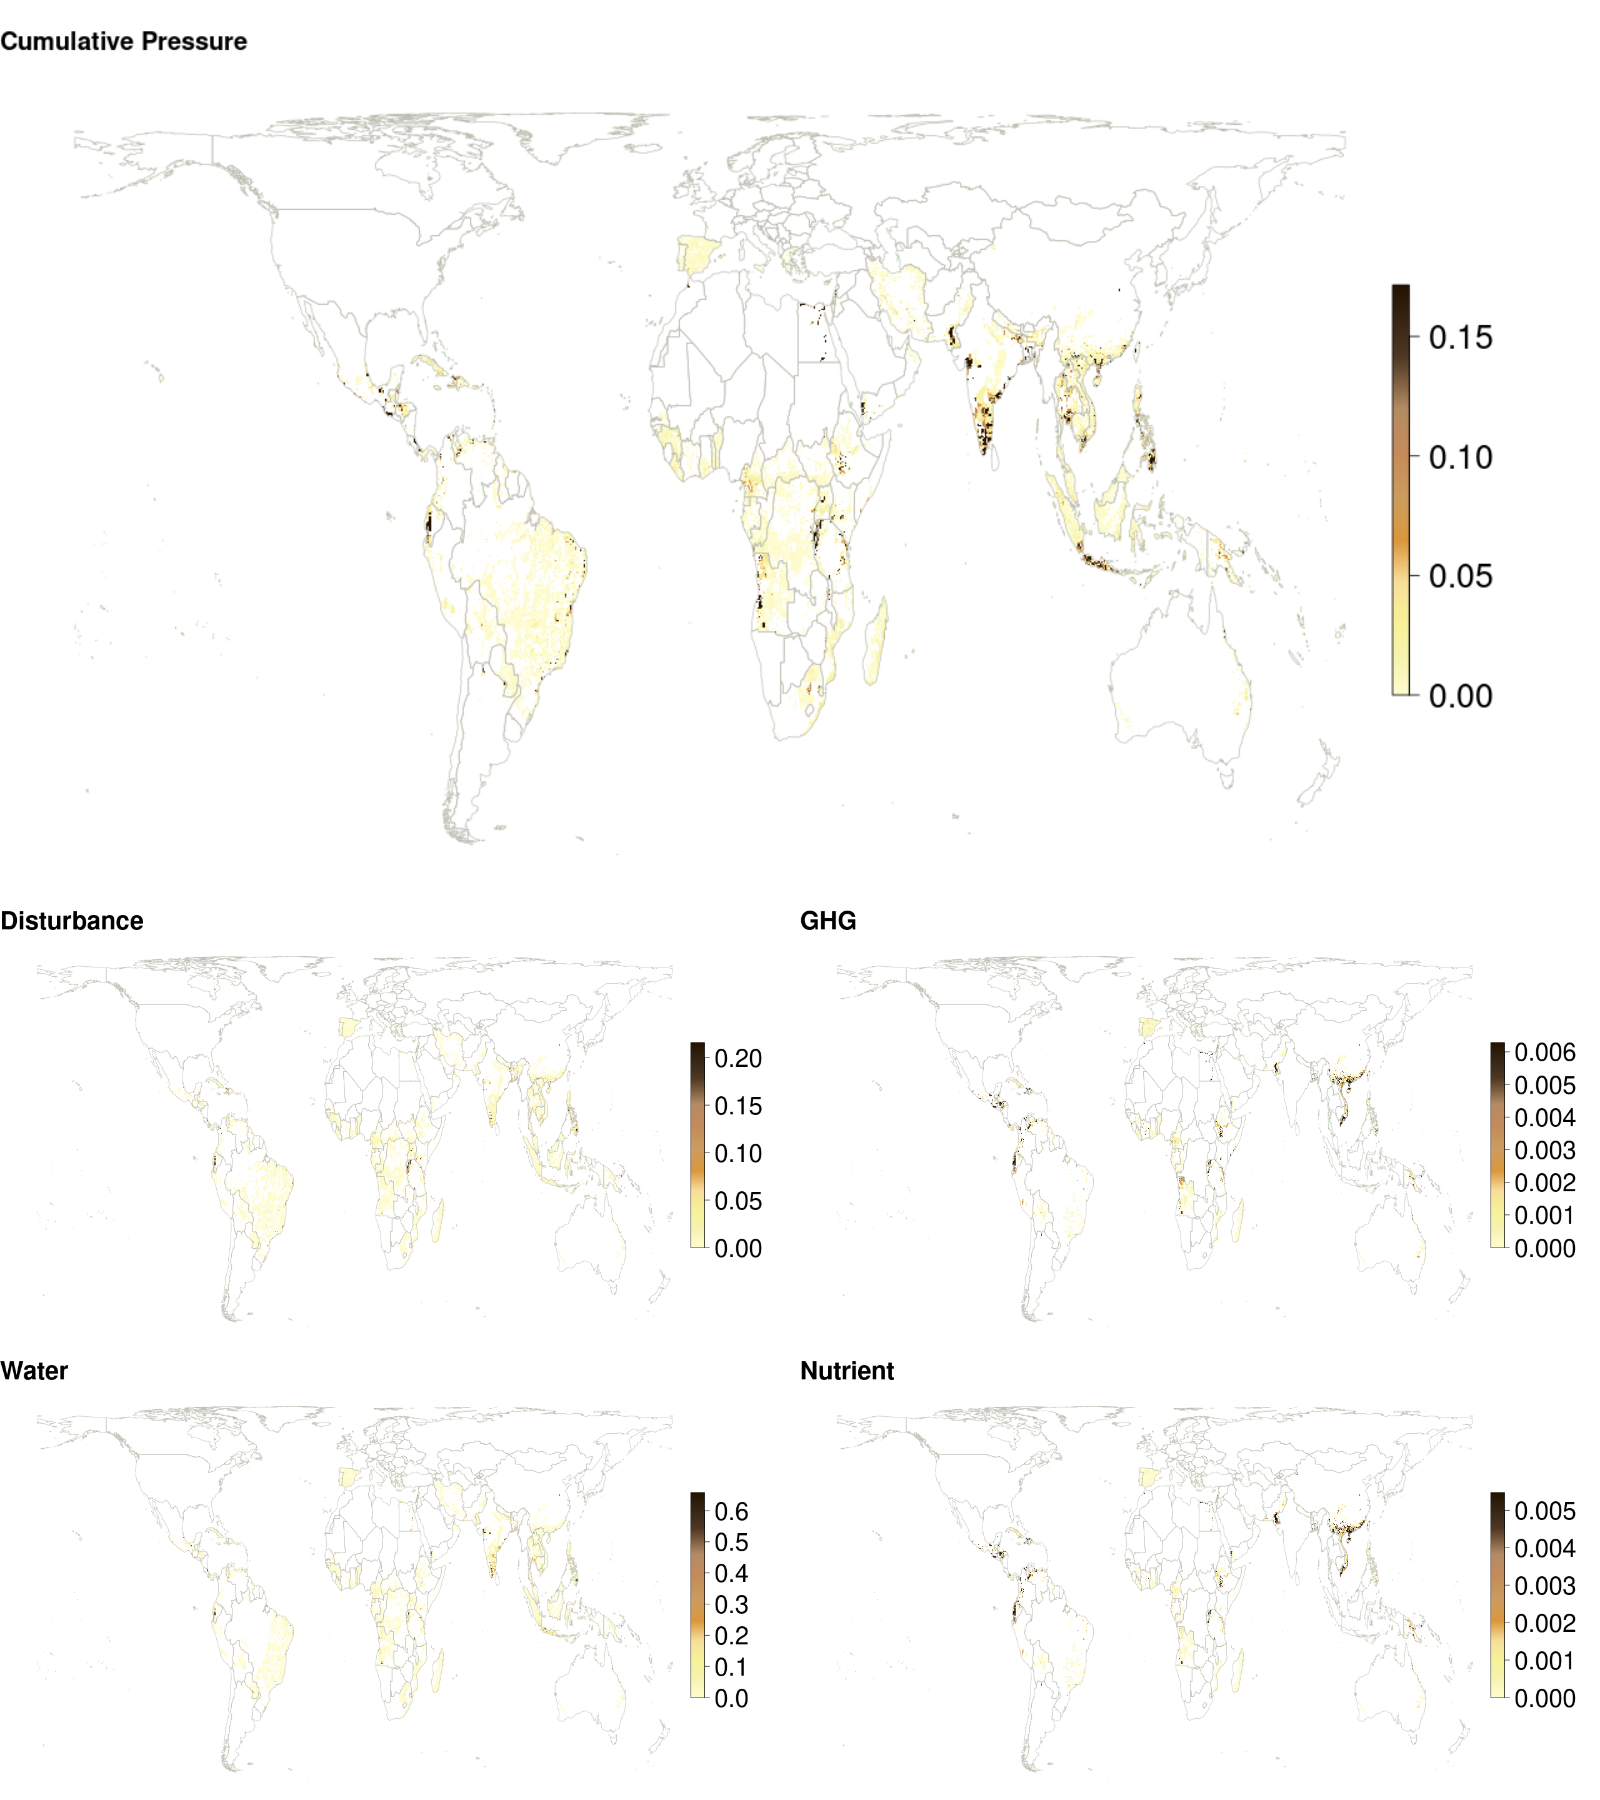
\includegraphics{/home/rayner/food-systems/_analysis/figures/extended_data/output/ed_fig_1_png/bana_crop_final.png}

\begin{center}\rule{0.5\linewidth}{0.5pt}\end{center}

\hypertarget{barley}{%
\subparagraph{2) Barley}\label{barley}}

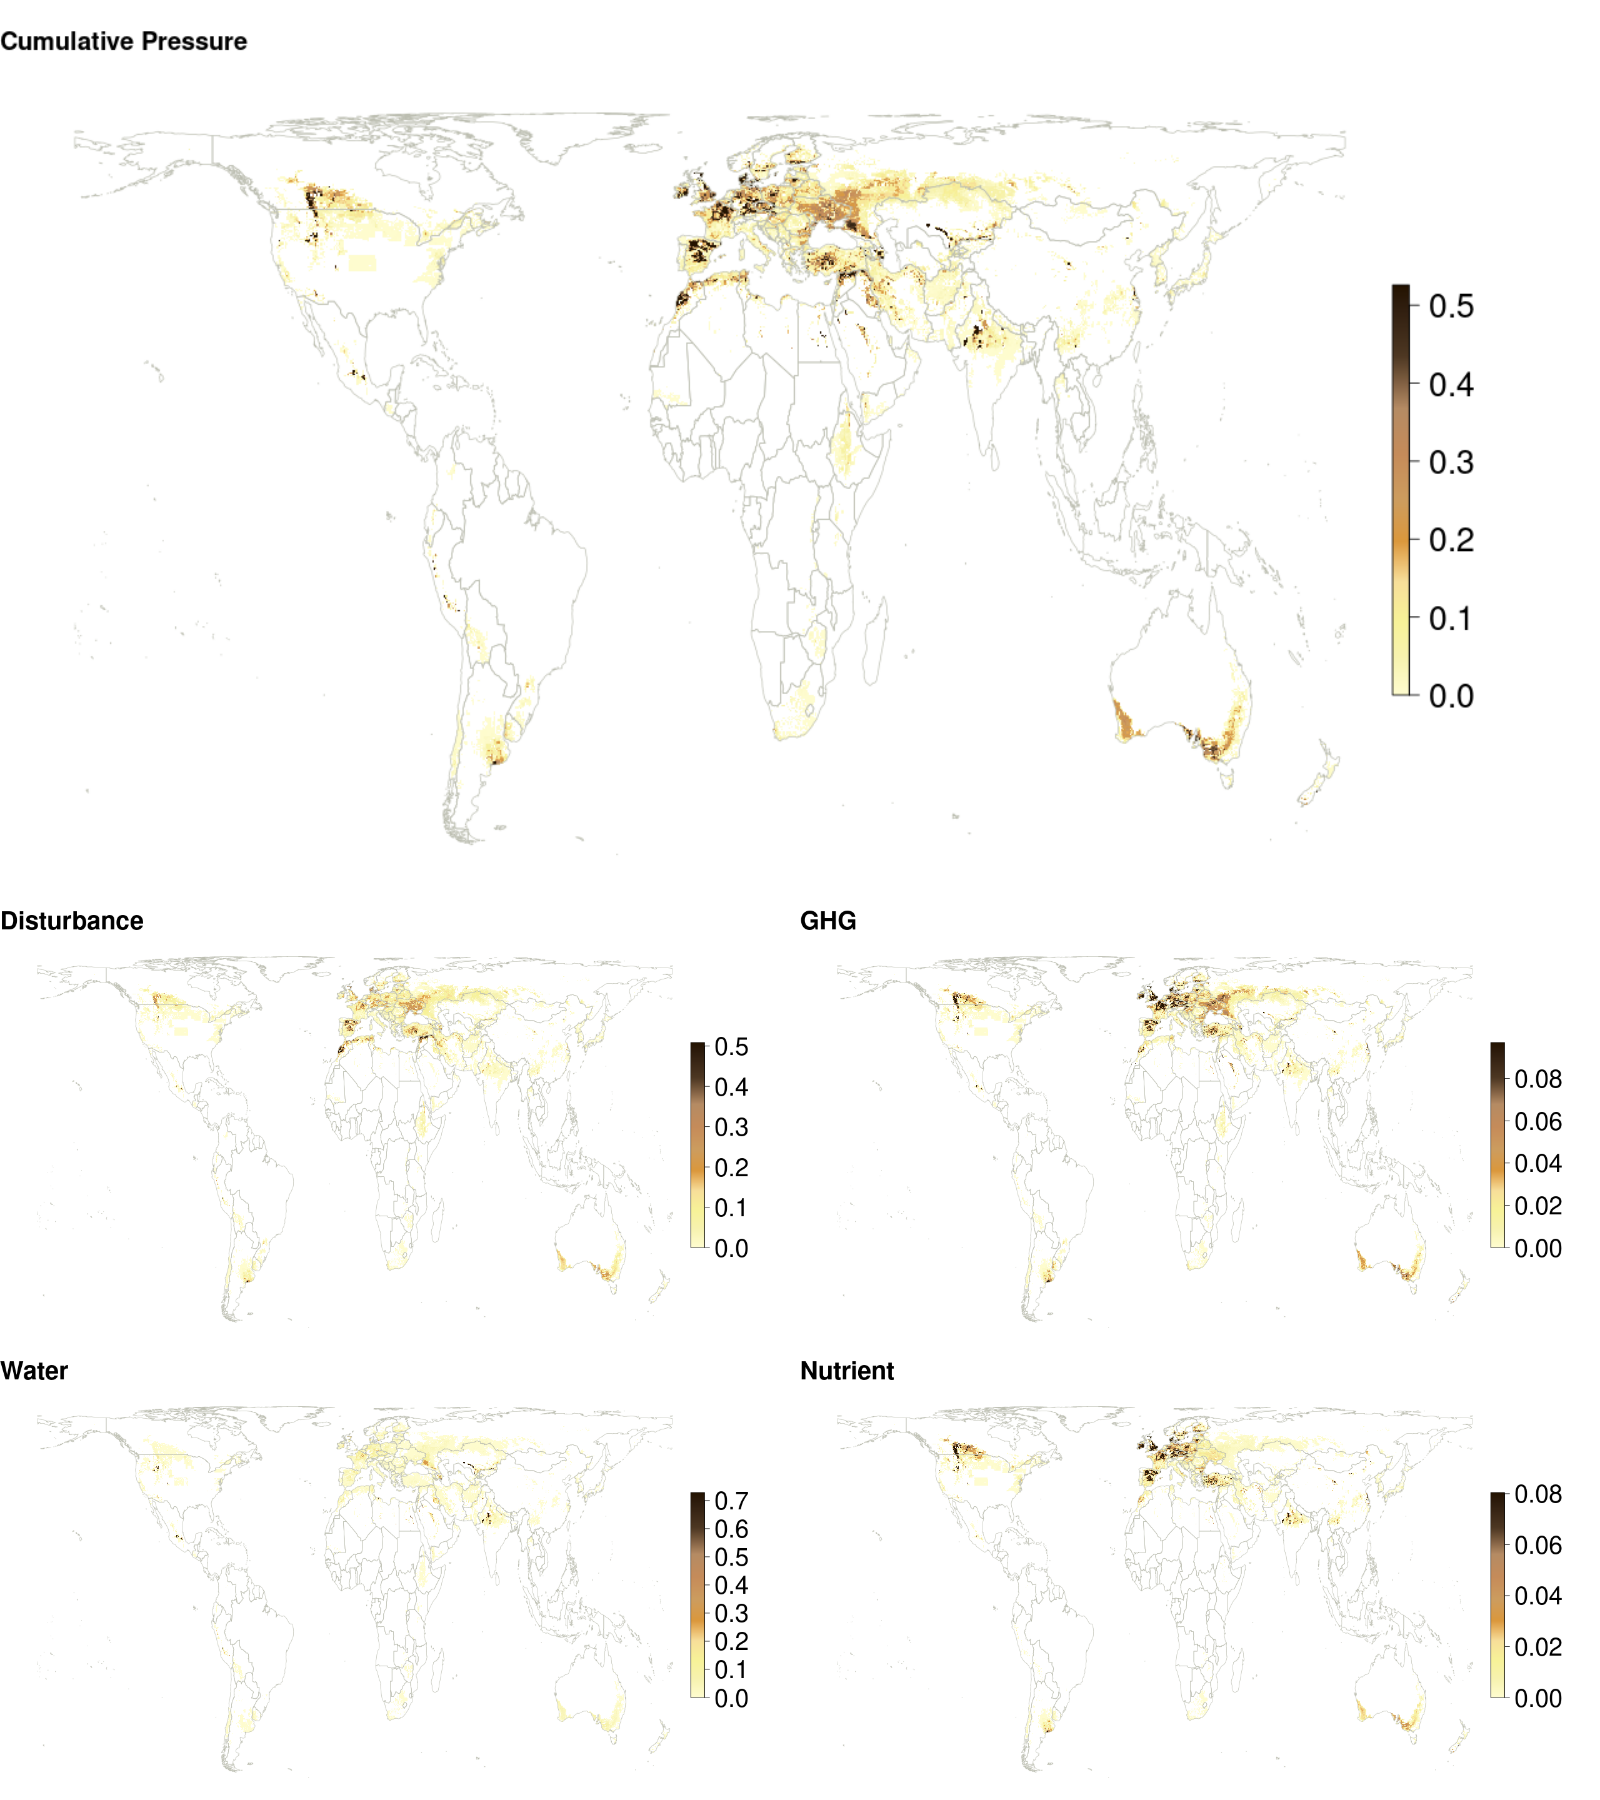
\includegraphics{/home/rayner/food-systems/_analysis/figures/extended_data/output/ed_fig_1_png/barl_crop_final.png}

\begin{center}\rule{0.5\linewidth}{0.5pt}\end{center}

\hypertarget{cassava}{%
\subparagraph{3) Cassava}\label{cassava}}

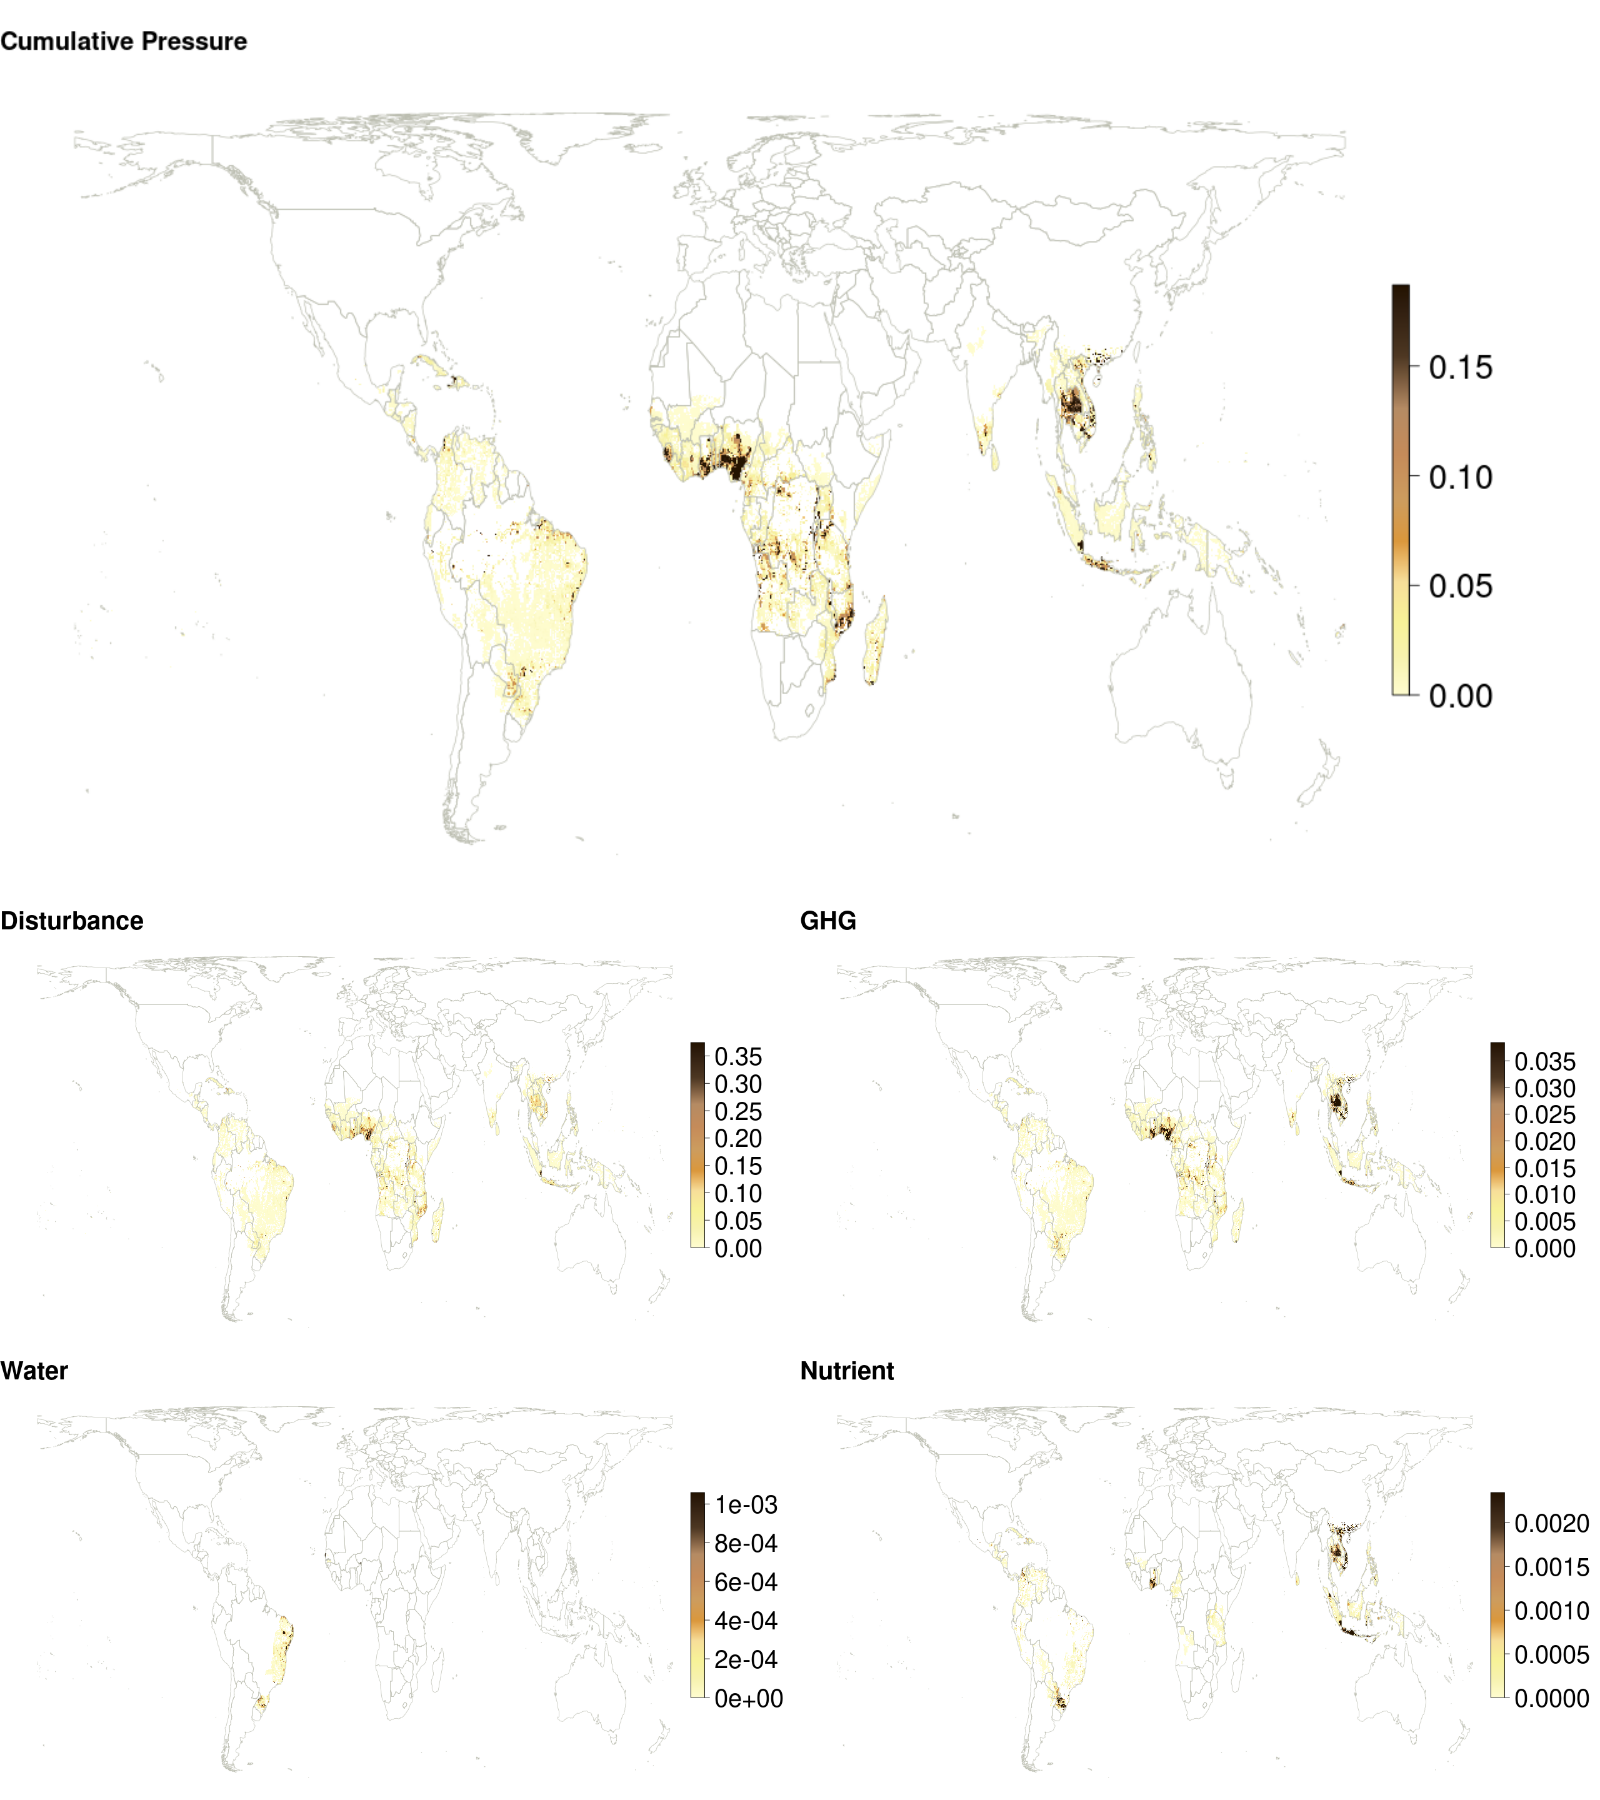
\includegraphics{/home/rayner/food-systems/_analysis/figures/extended_data/output/ed_fig_1_png/cass_crop_final.png}

\begin{center}\rule{0.5\linewidth}{0.5pt}\end{center}

\hypertarget{coconut}{%
\subparagraph{4) Coconut}\label{coconut}}

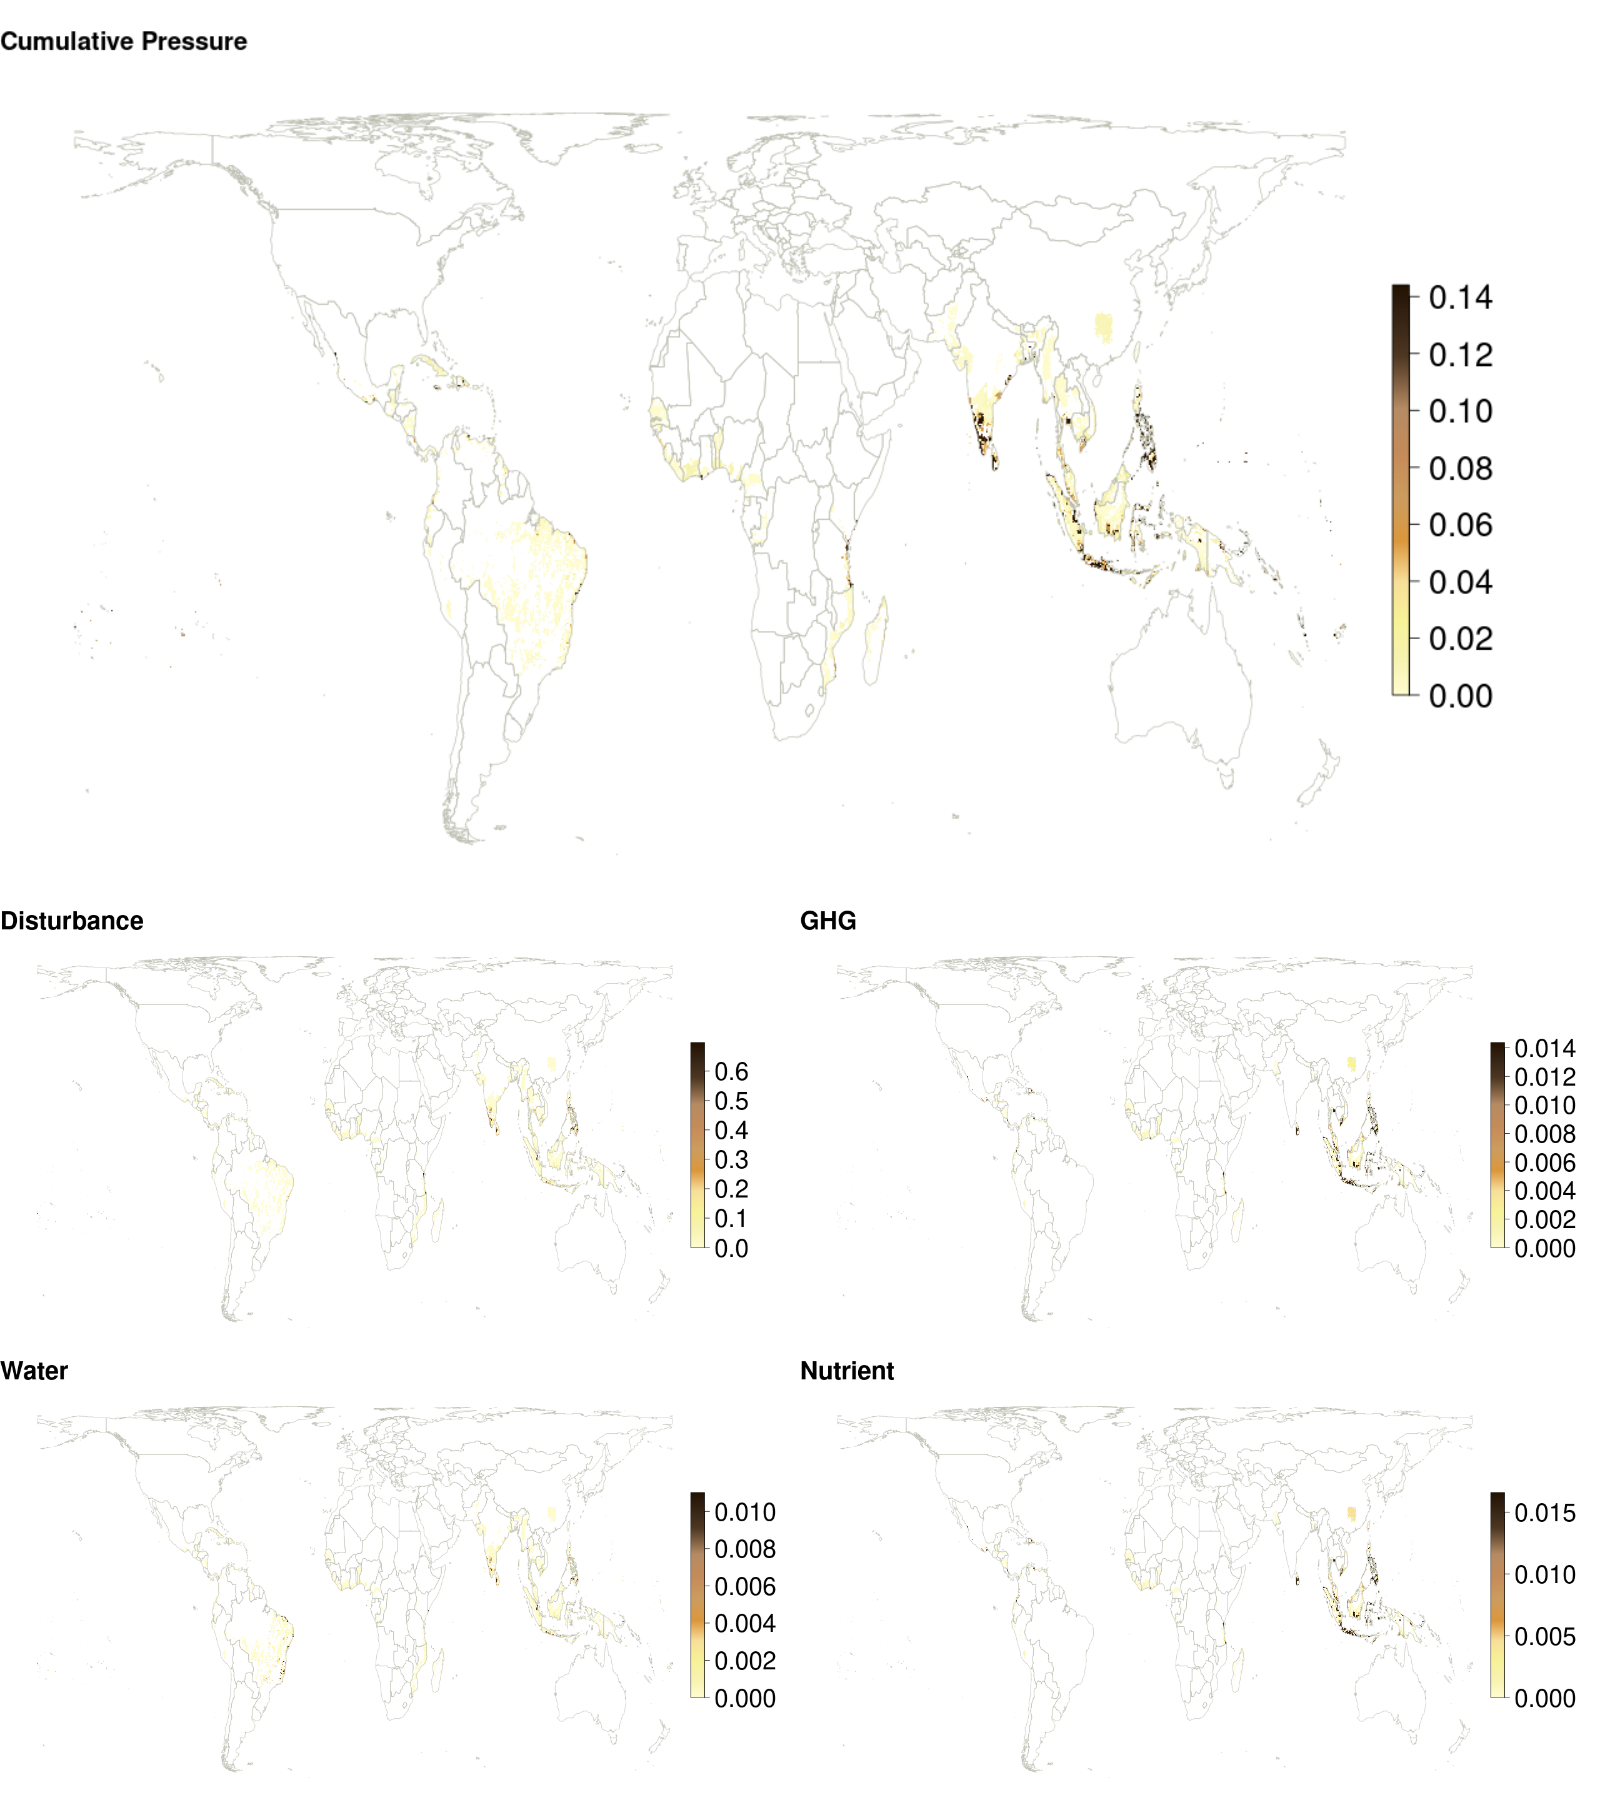
\includegraphics{/home/rayner/food-systems/_analysis/figures/extended_data/output/ed_fig_1_png/cnut_crop_final.png}

\begin{center}\rule{0.5\linewidth}{0.5pt}\end{center}

\hypertarget{cocoa}{%
\subparagraph{5) Cocoa}\label{cocoa}}

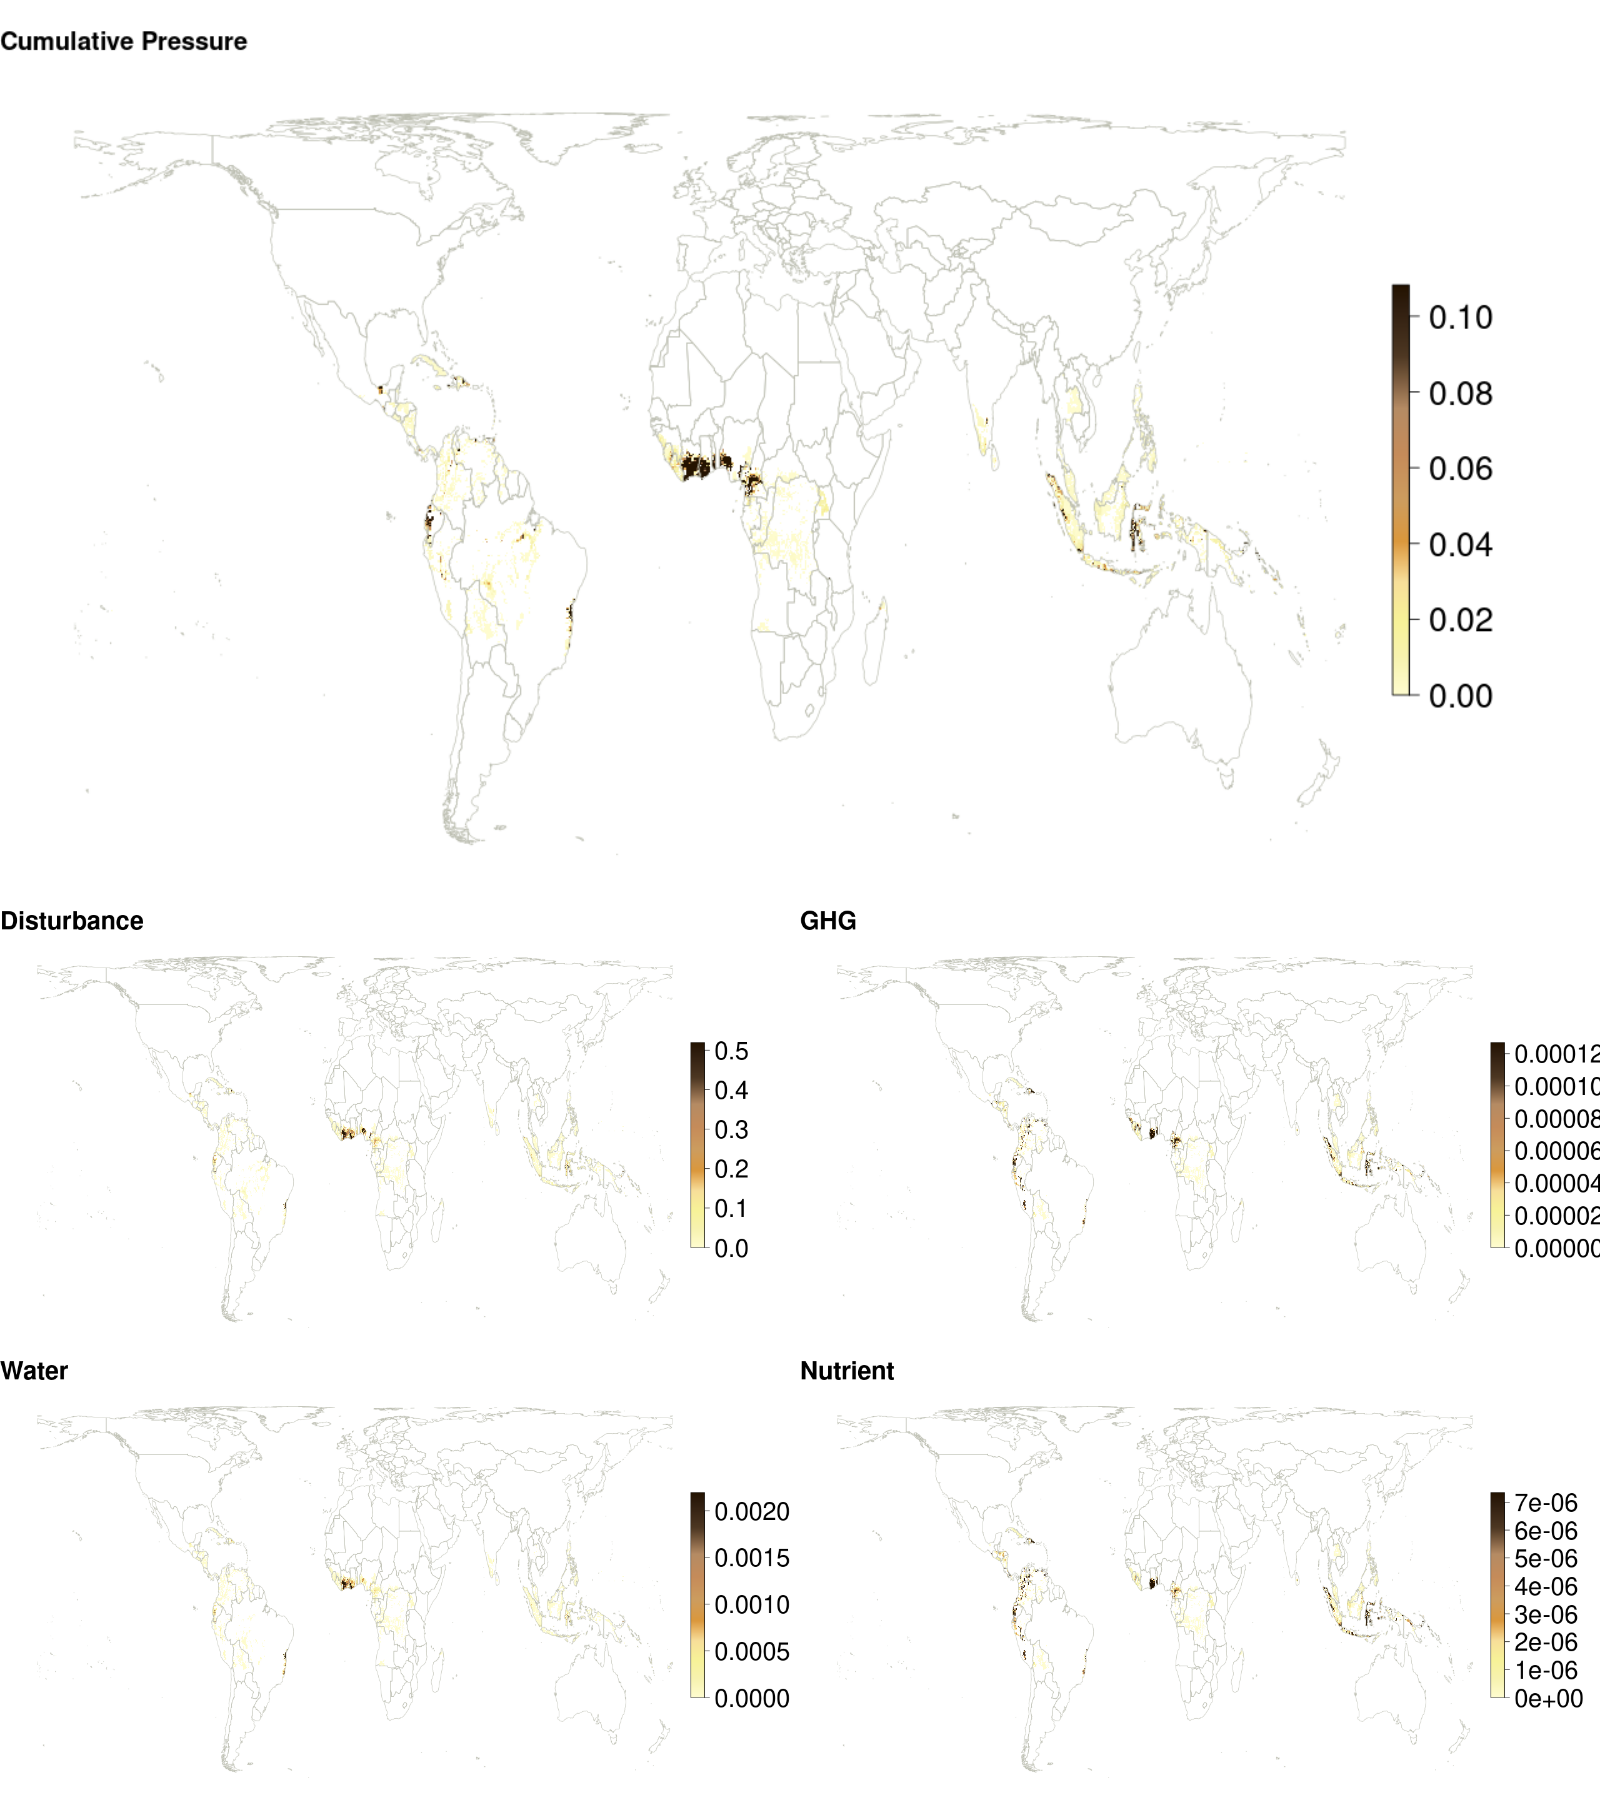
\includegraphics{/home/rayner/food-systems/_analysis/figures/extended_data/output/ed_fig_1_png/coco_crop_final.png}

\begin{center}\rule{0.5\linewidth}{0.5pt}\end{center}

\hypertarget{fodder}{%
\subparagraph{6) Fodder}\label{fodder}}

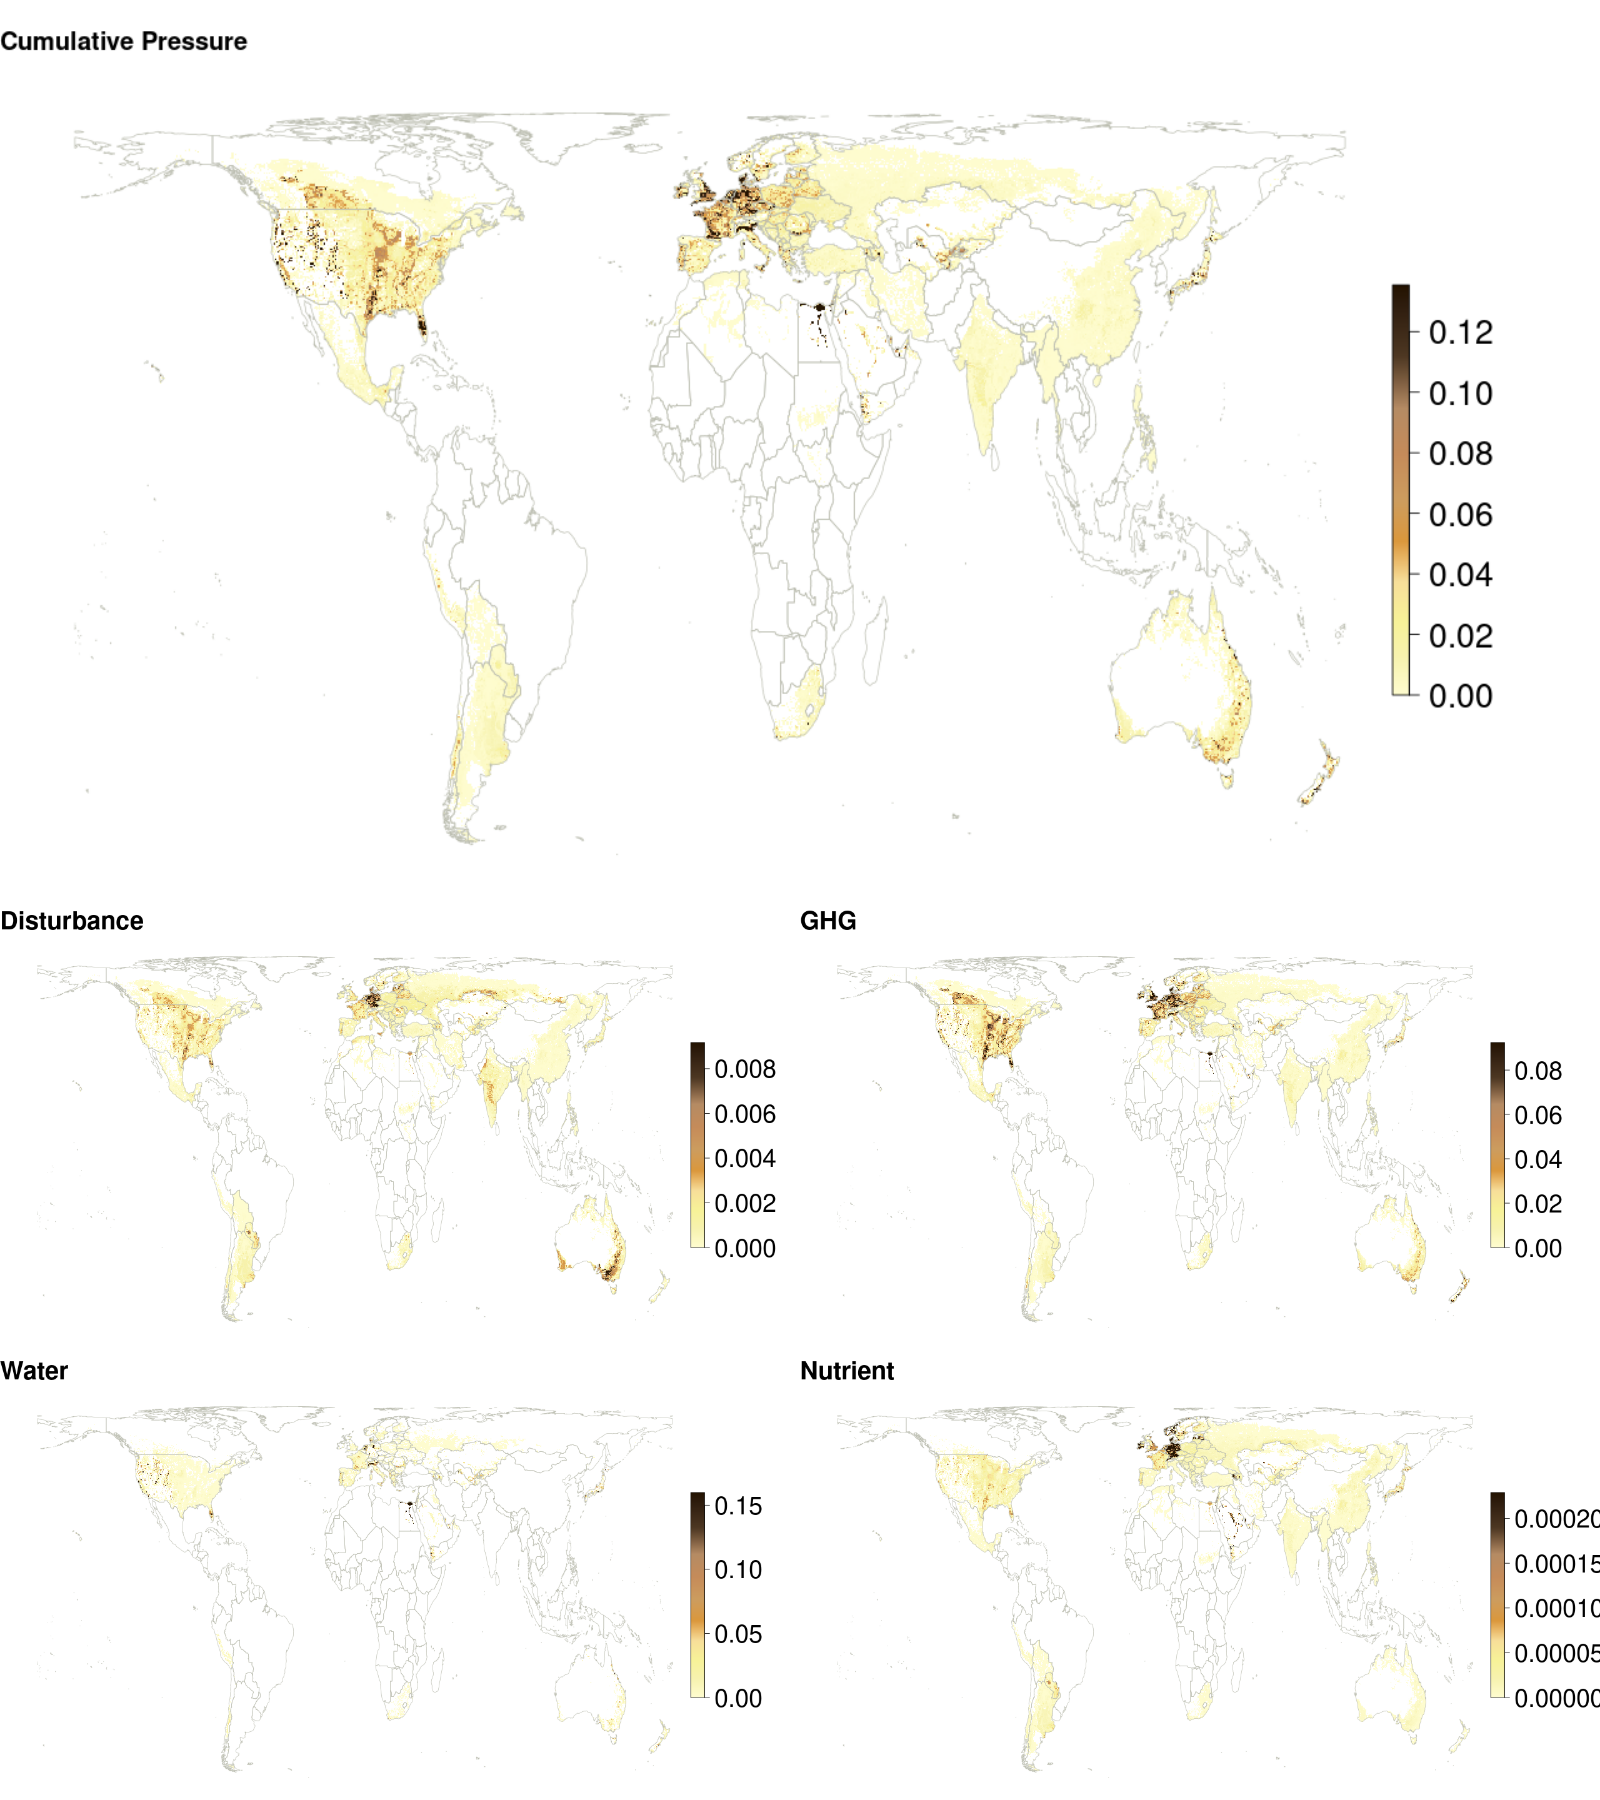
\includegraphics{/home/rayner/food-systems/_analysis/figures/extended_data/output/ed_fig_1_png/fodd_crop_final.png}

\begin{center}\rule{0.5\linewidth}{0.5pt}\end{center}

\hypertarget{maize}{%
\subparagraph{7) Maize}\label{maize}}

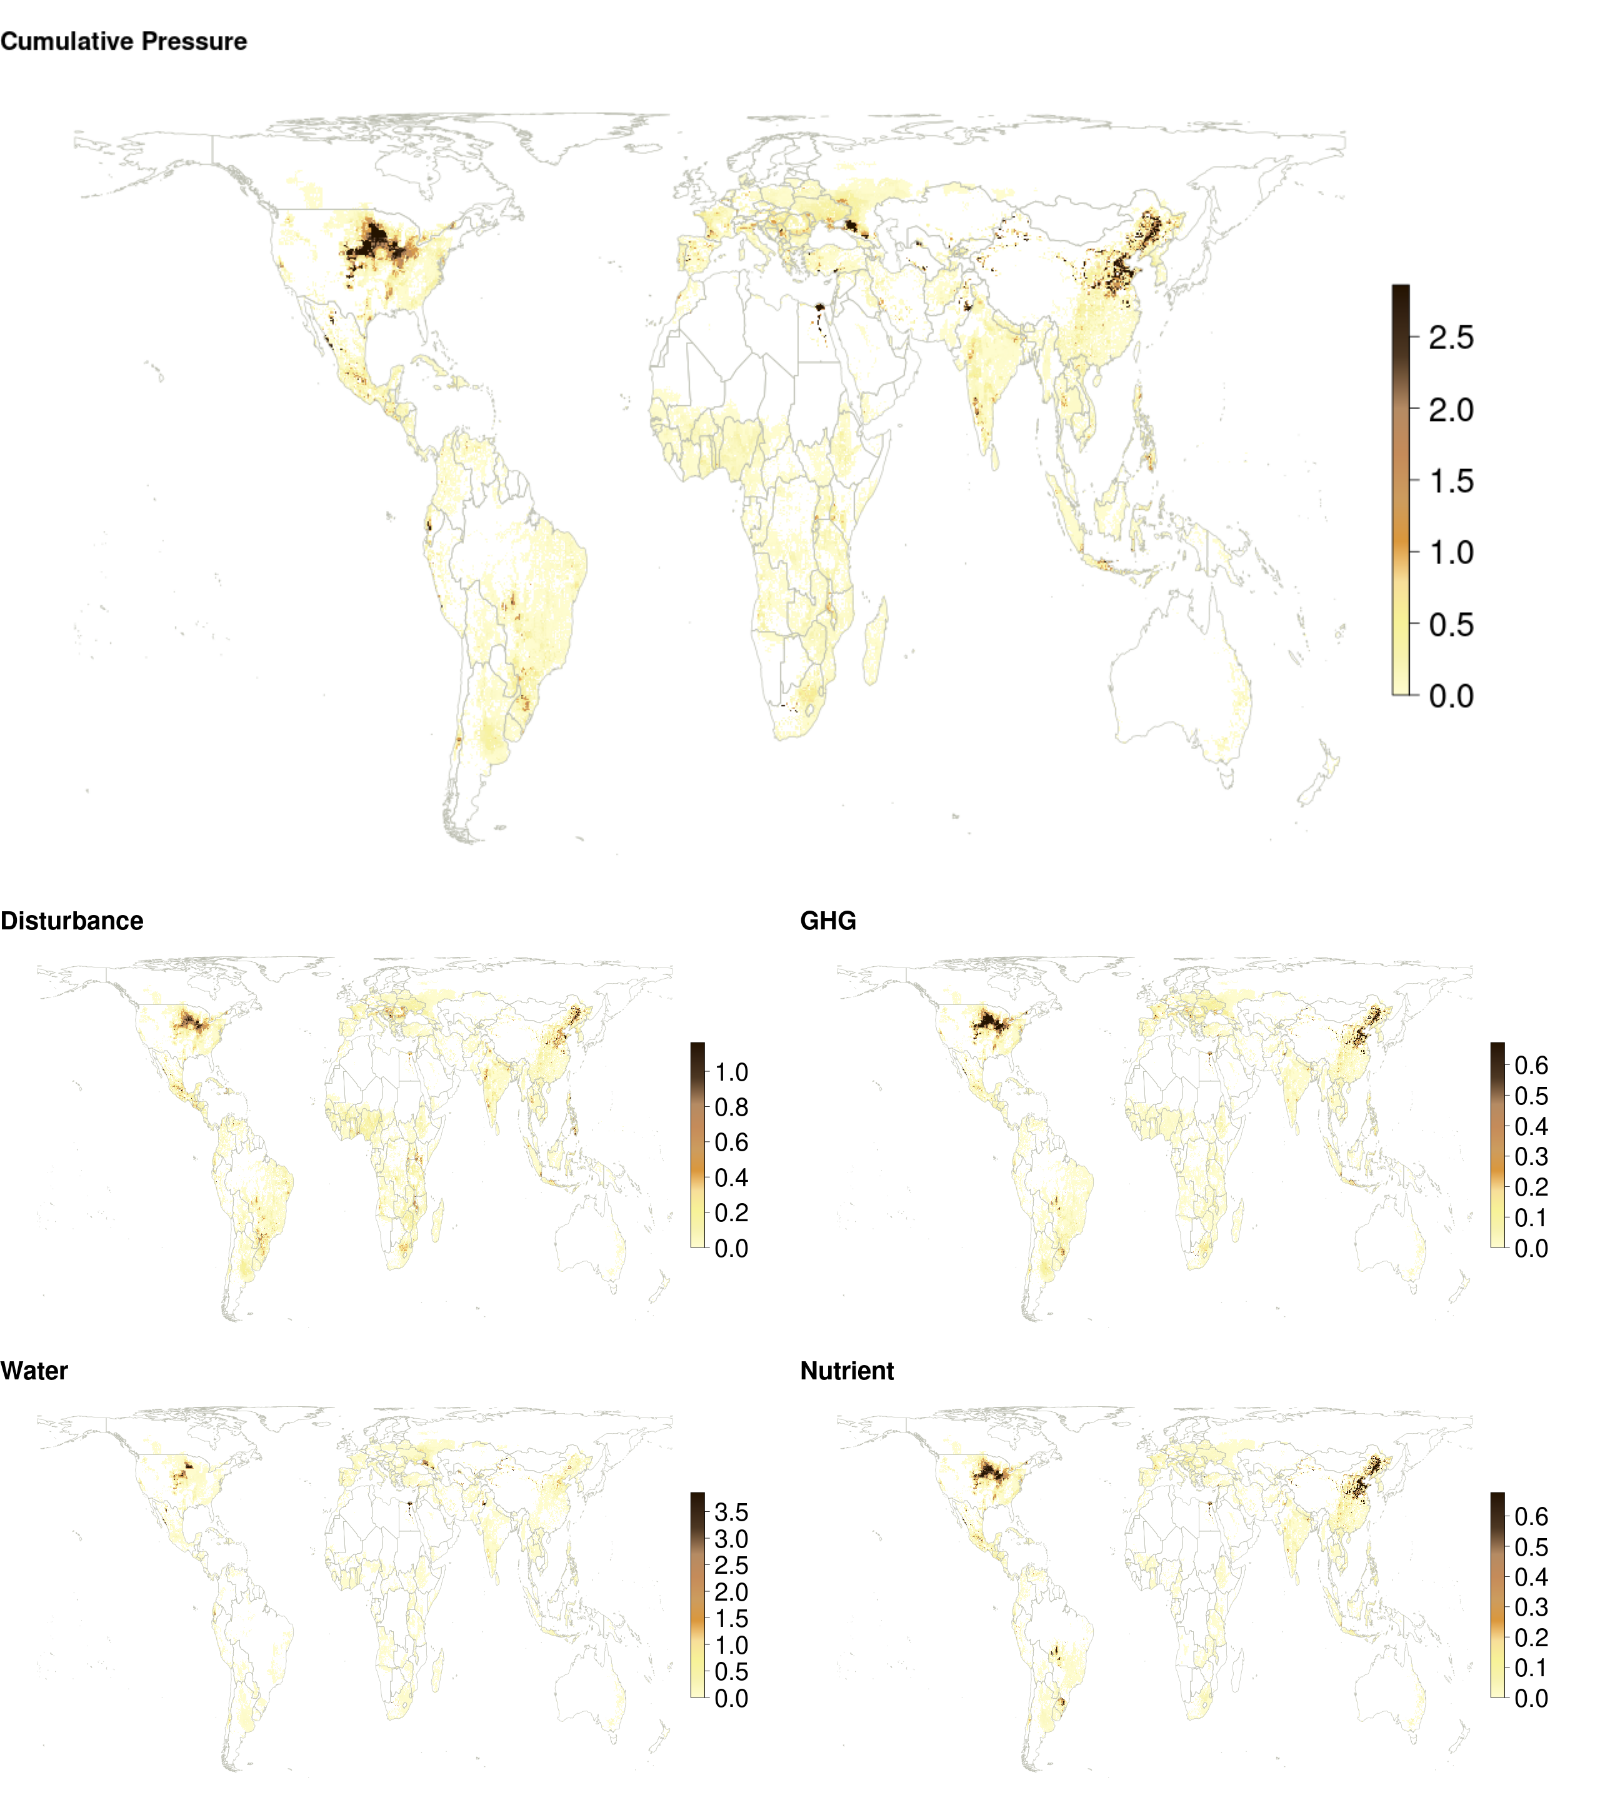
\includegraphics{/home/rayner/food-systems/_analysis/figures/extended_data/output/ed_fig_1_png/maiz_crop_final.png}

\begin{center}\rule{0.5\linewidth}{0.5pt}\end{center}

\hypertarget{other-cereals}{%
\subparagraph{8) Other cereals}\label{other-cereals}}

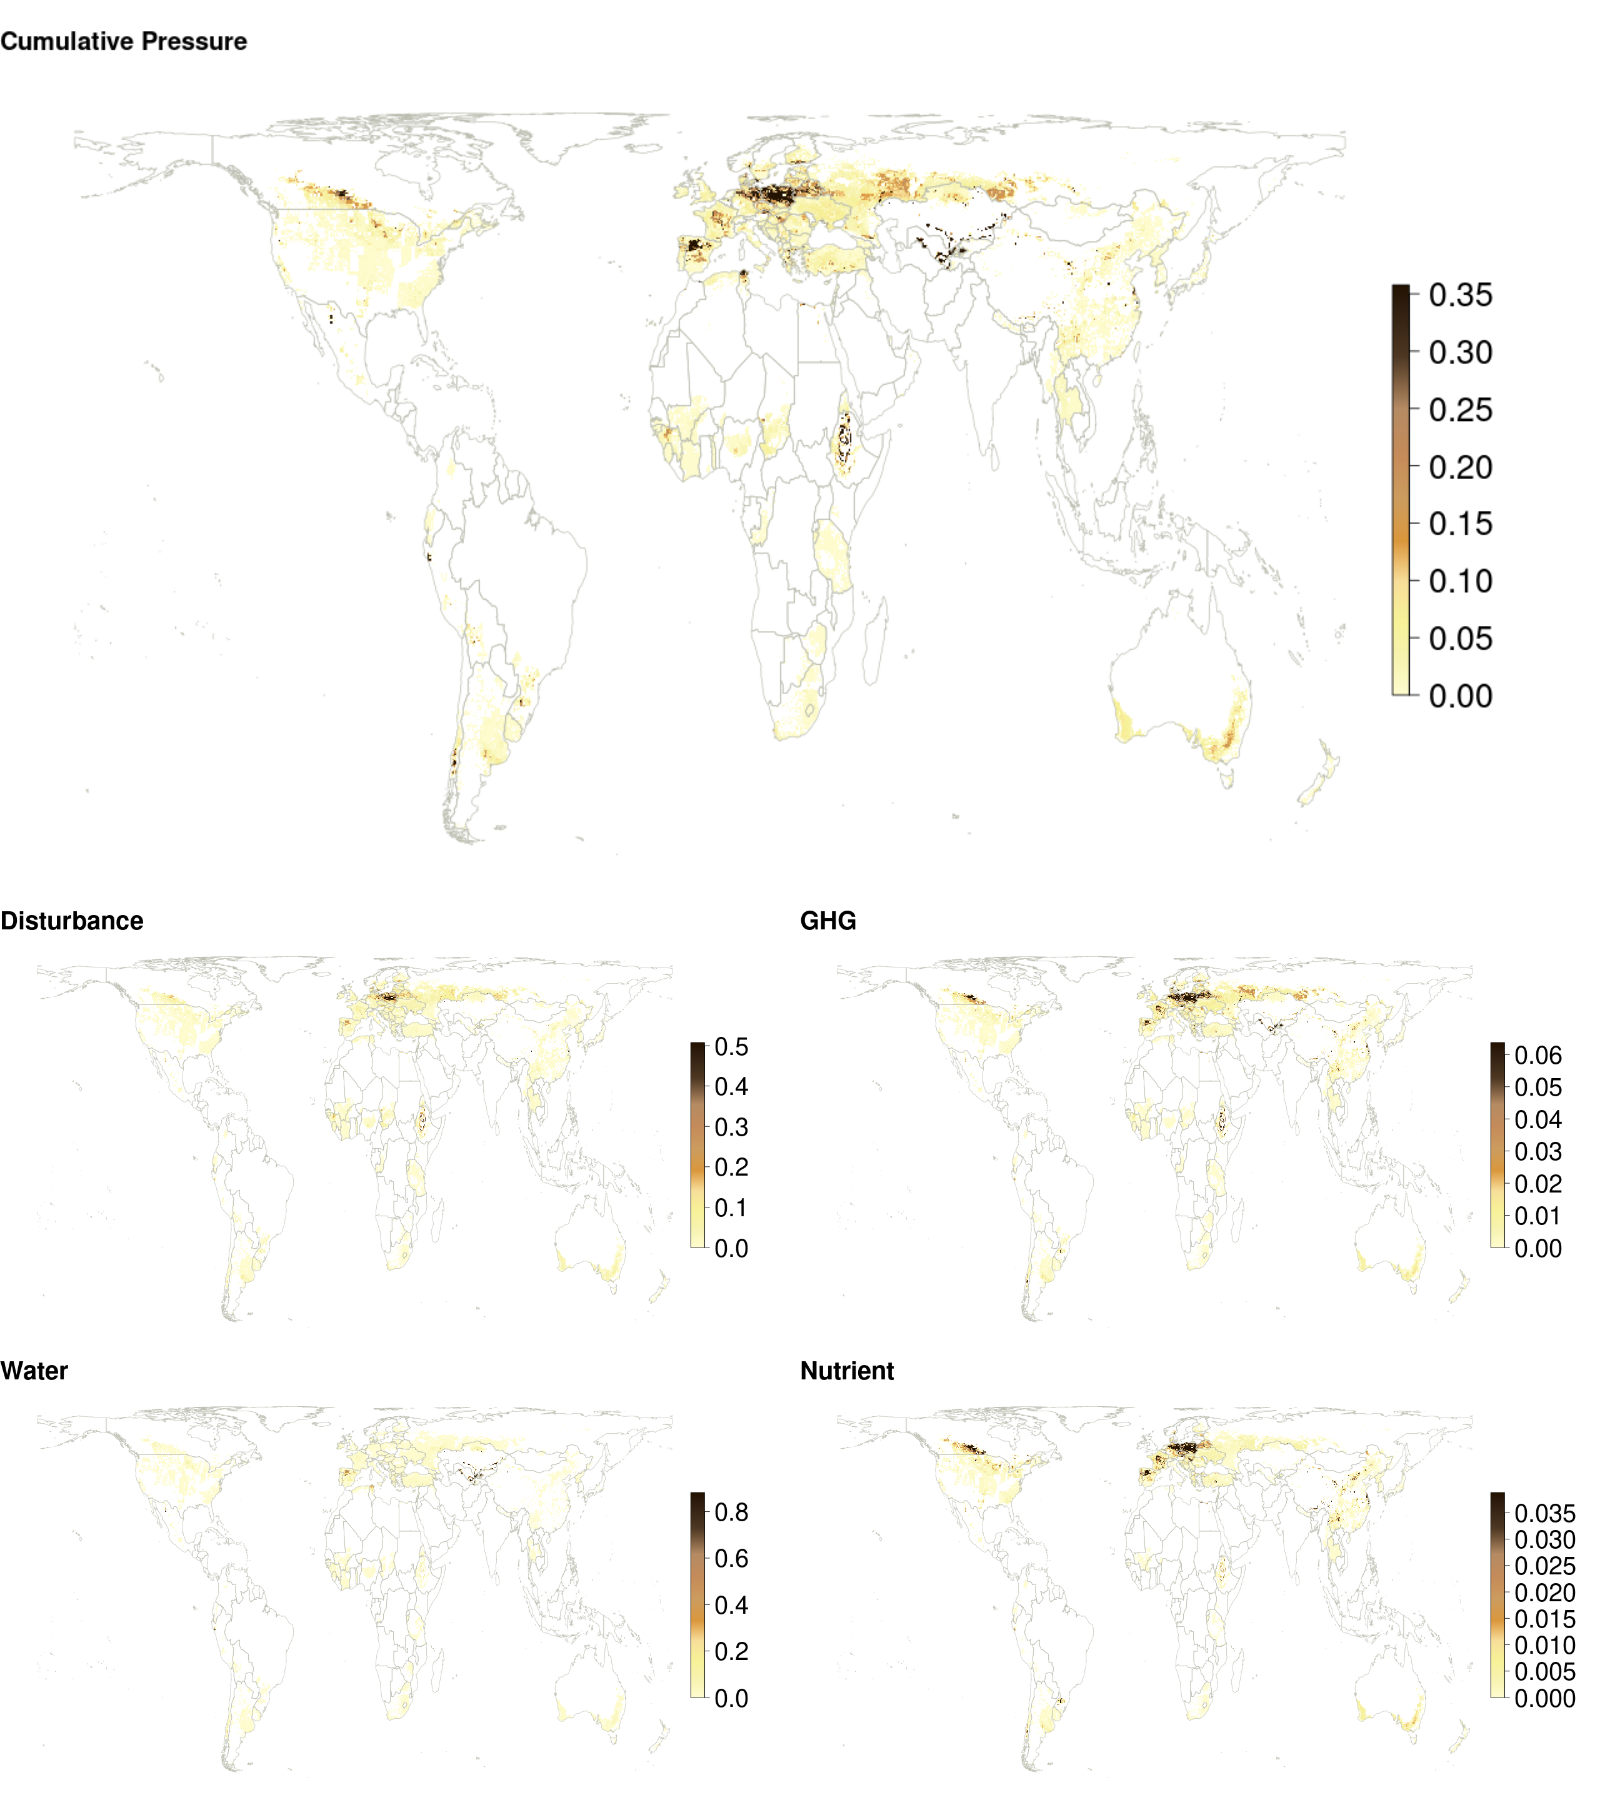
\includegraphics{/home/rayner/food-systems/_analysis/figures/extended_data/output/ed_fig_1_png/ocer_crop_final.png}

\begin{center}\rule{0.5\linewidth}{0.5pt}\end{center}

\hypertarget{oilpalm}{%
\subparagraph{9) Oilpalm}\label{oilpalm}}

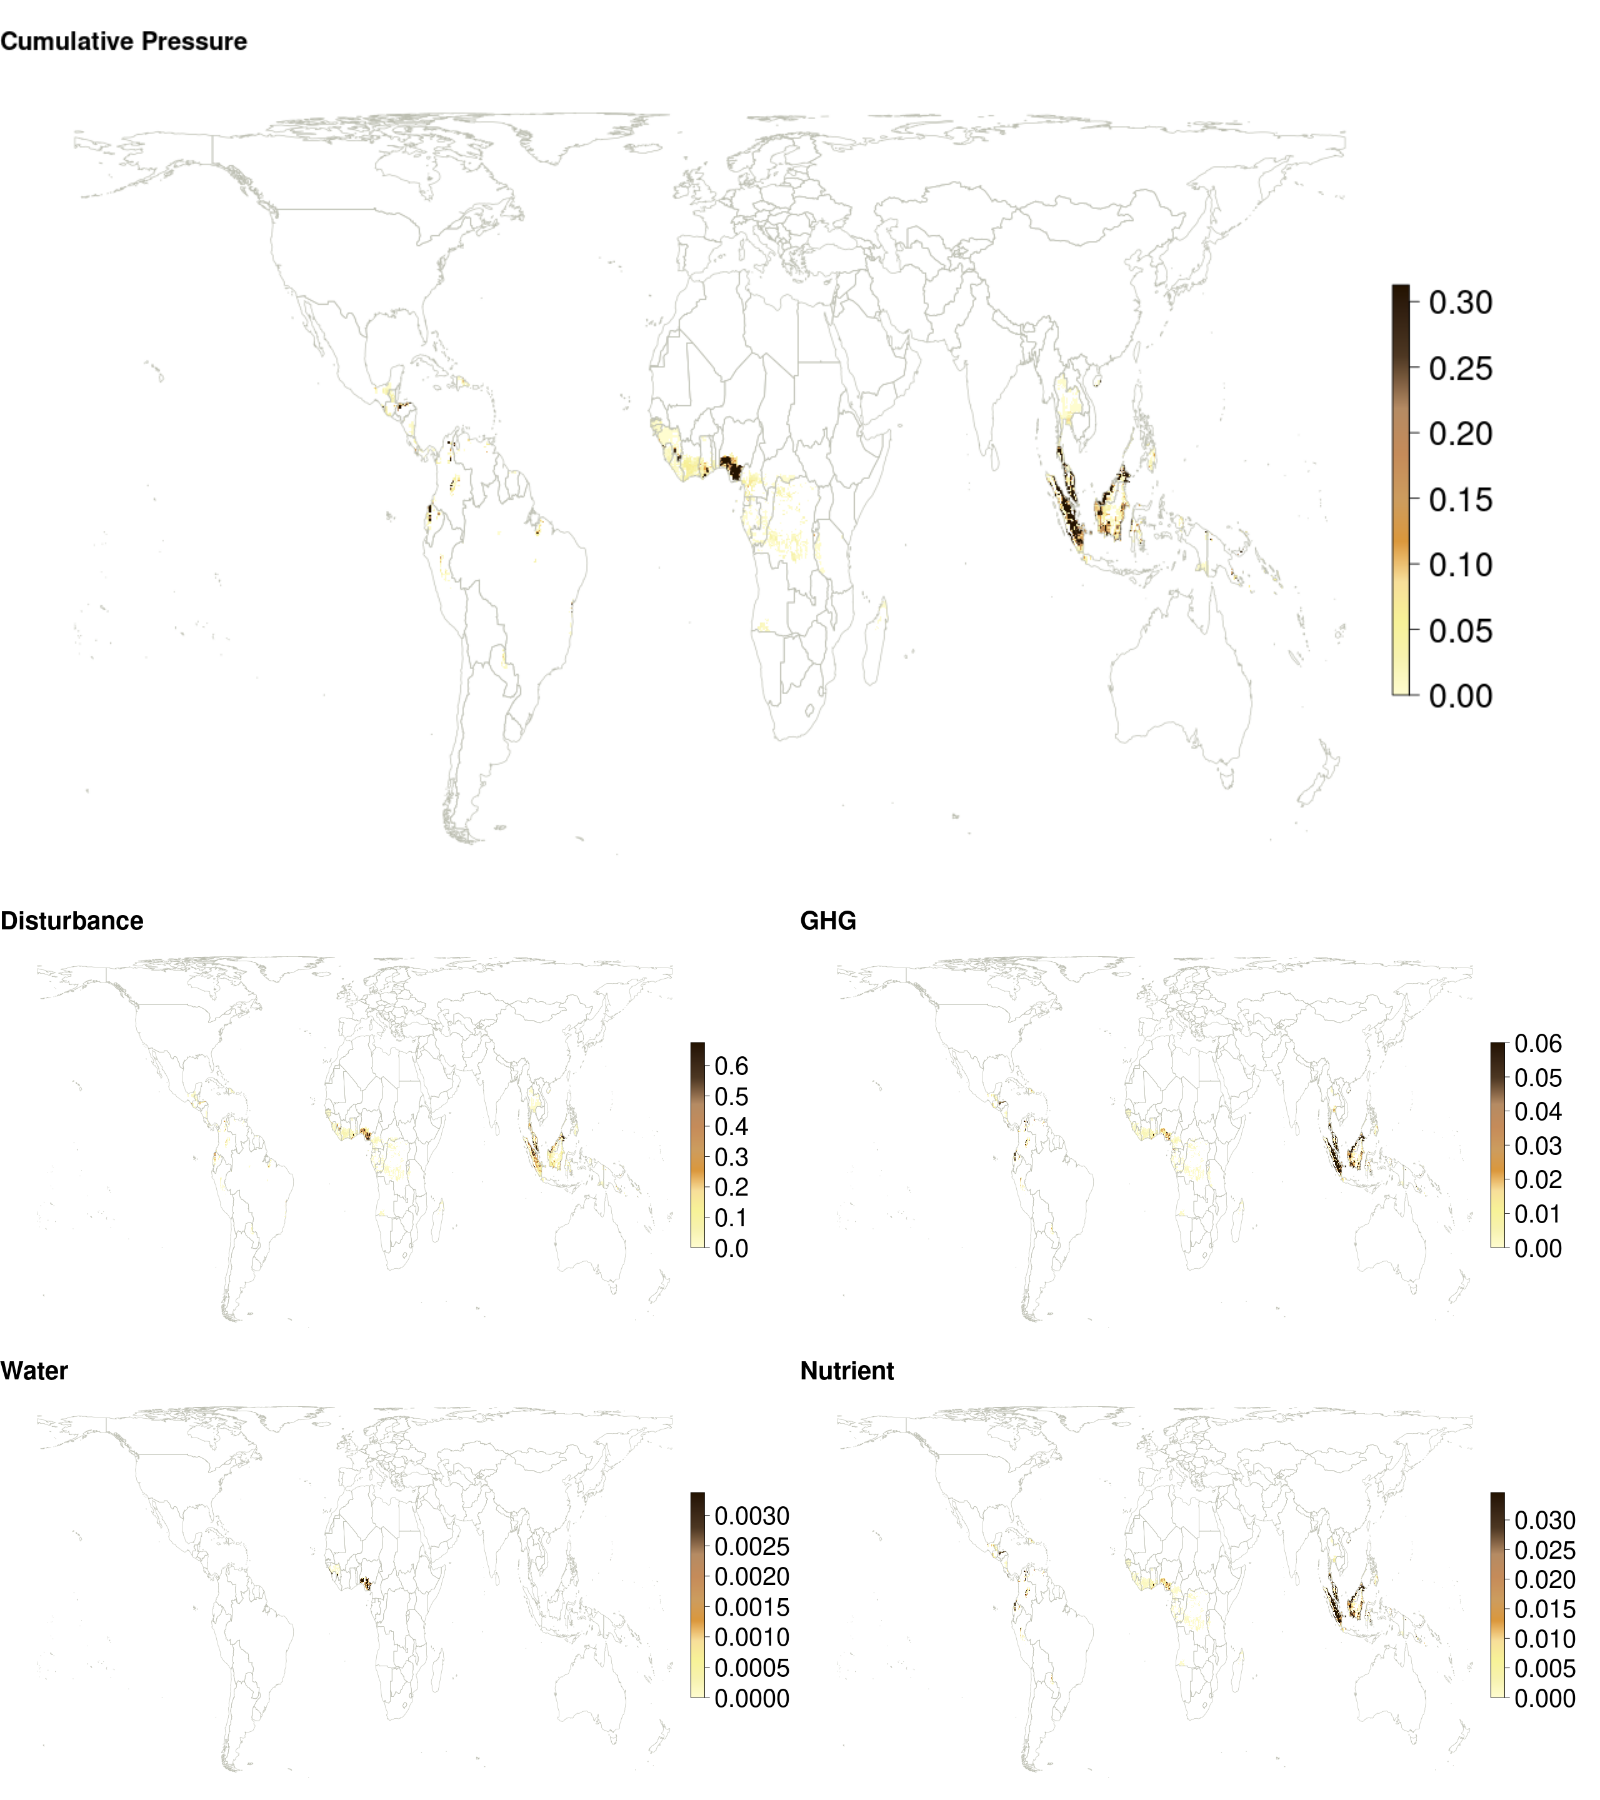
\includegraphics{/home/rayner/food-systems/_analysis/figures/extended_data/output/ed_fig_1_png/oilp_crop_final.png}

\begin{center}\rule{0.5\linewidth}{0.5pt}\end{center}

\hypertarget{other-roots}{%
\subparagraph{10) Other roots}\label{other-roots}}

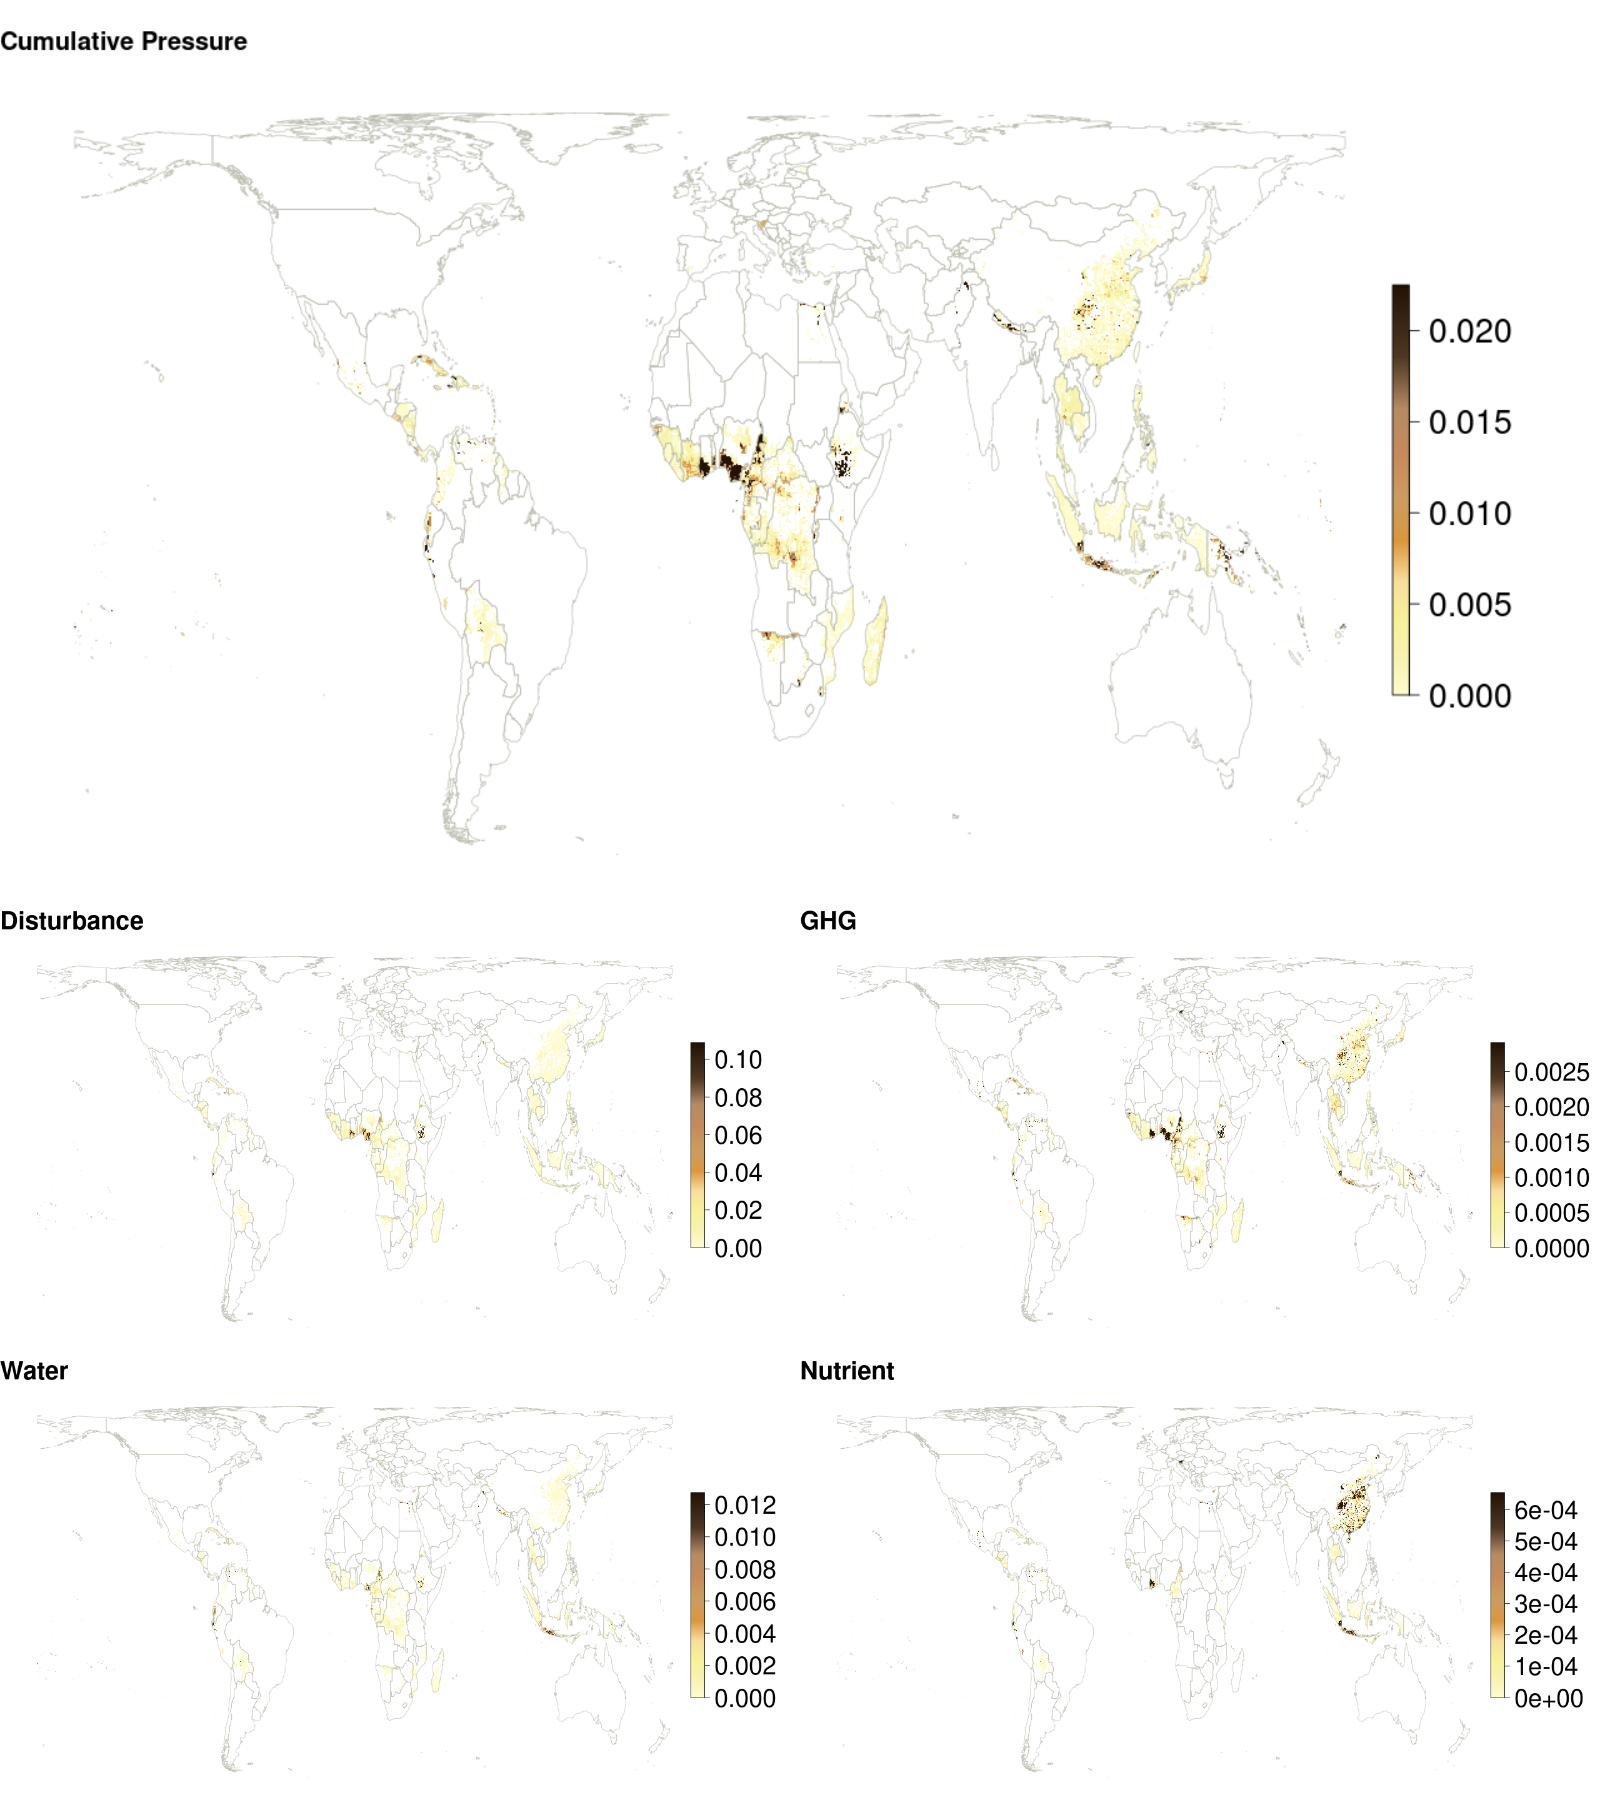
\includegraphics{/home/rayner/food-systems/_analysis/figures/extended_data/output/ed_fig_1_png/orts_crop_final.png}

\begin{center}\rule{0.5\linewidth}{0.5pt}\end{center}

\hypertarget{plantain}{%
\subparagraph{11) Plantain}\label{plantain}}

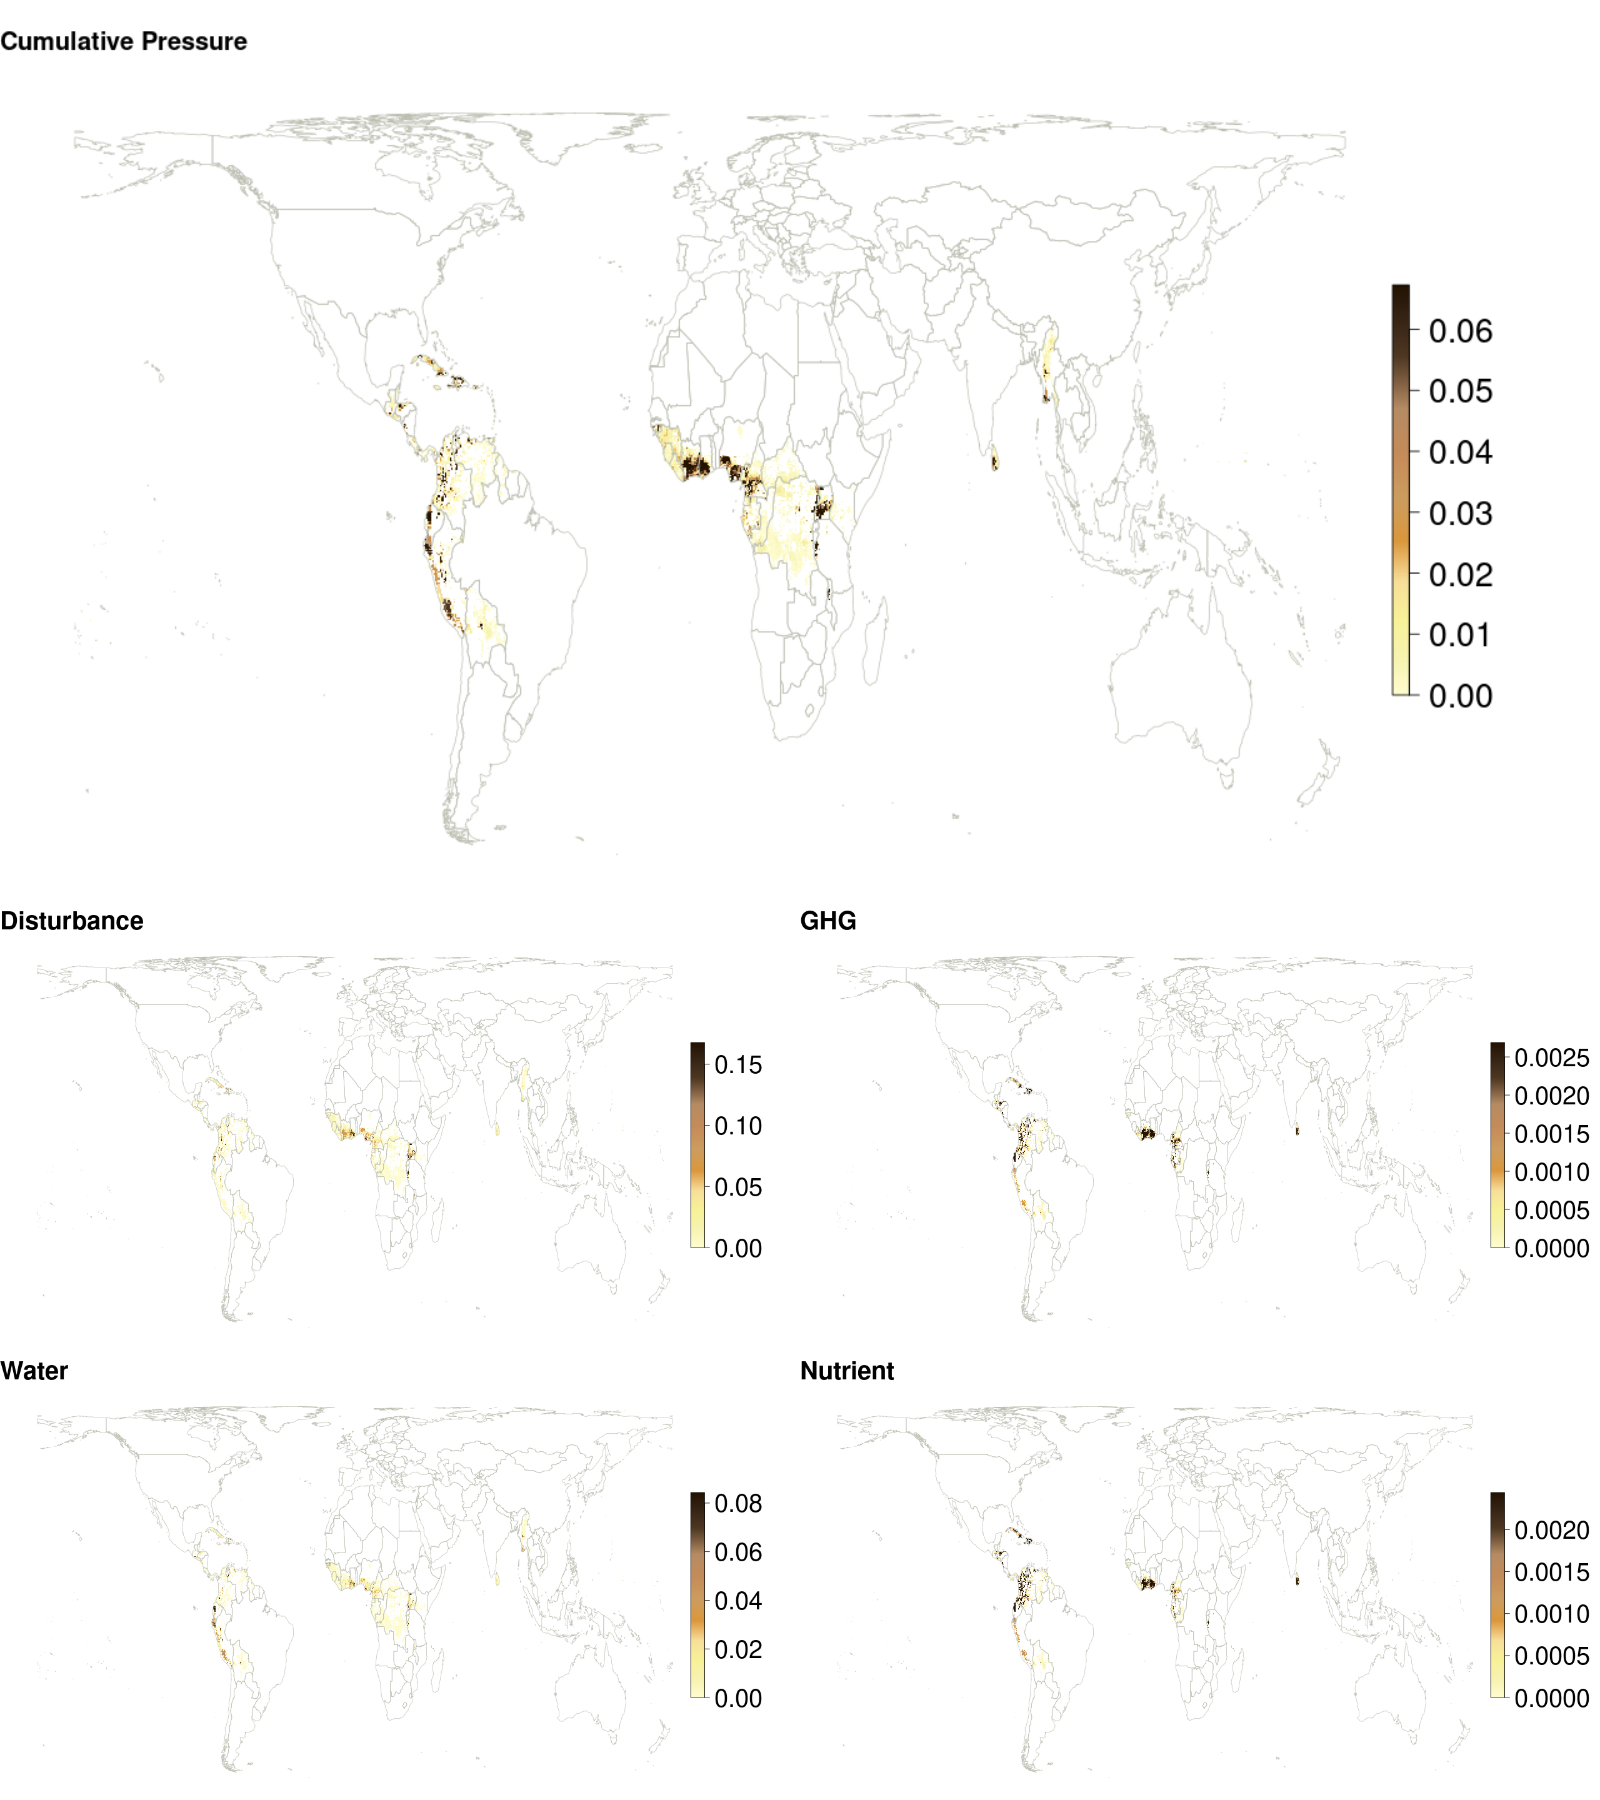
\includegraphics{/home/rayner/food-systems/_analysis/figures/extended_data/output/ed_fig_1_png/plnt_crop_final.png}

\begin{center}\rule{0.5\linewidth}{0.5pt}\end{center}

\hypertarget{potato}{%
\subparagraph{12) Potato}\label{potato}}

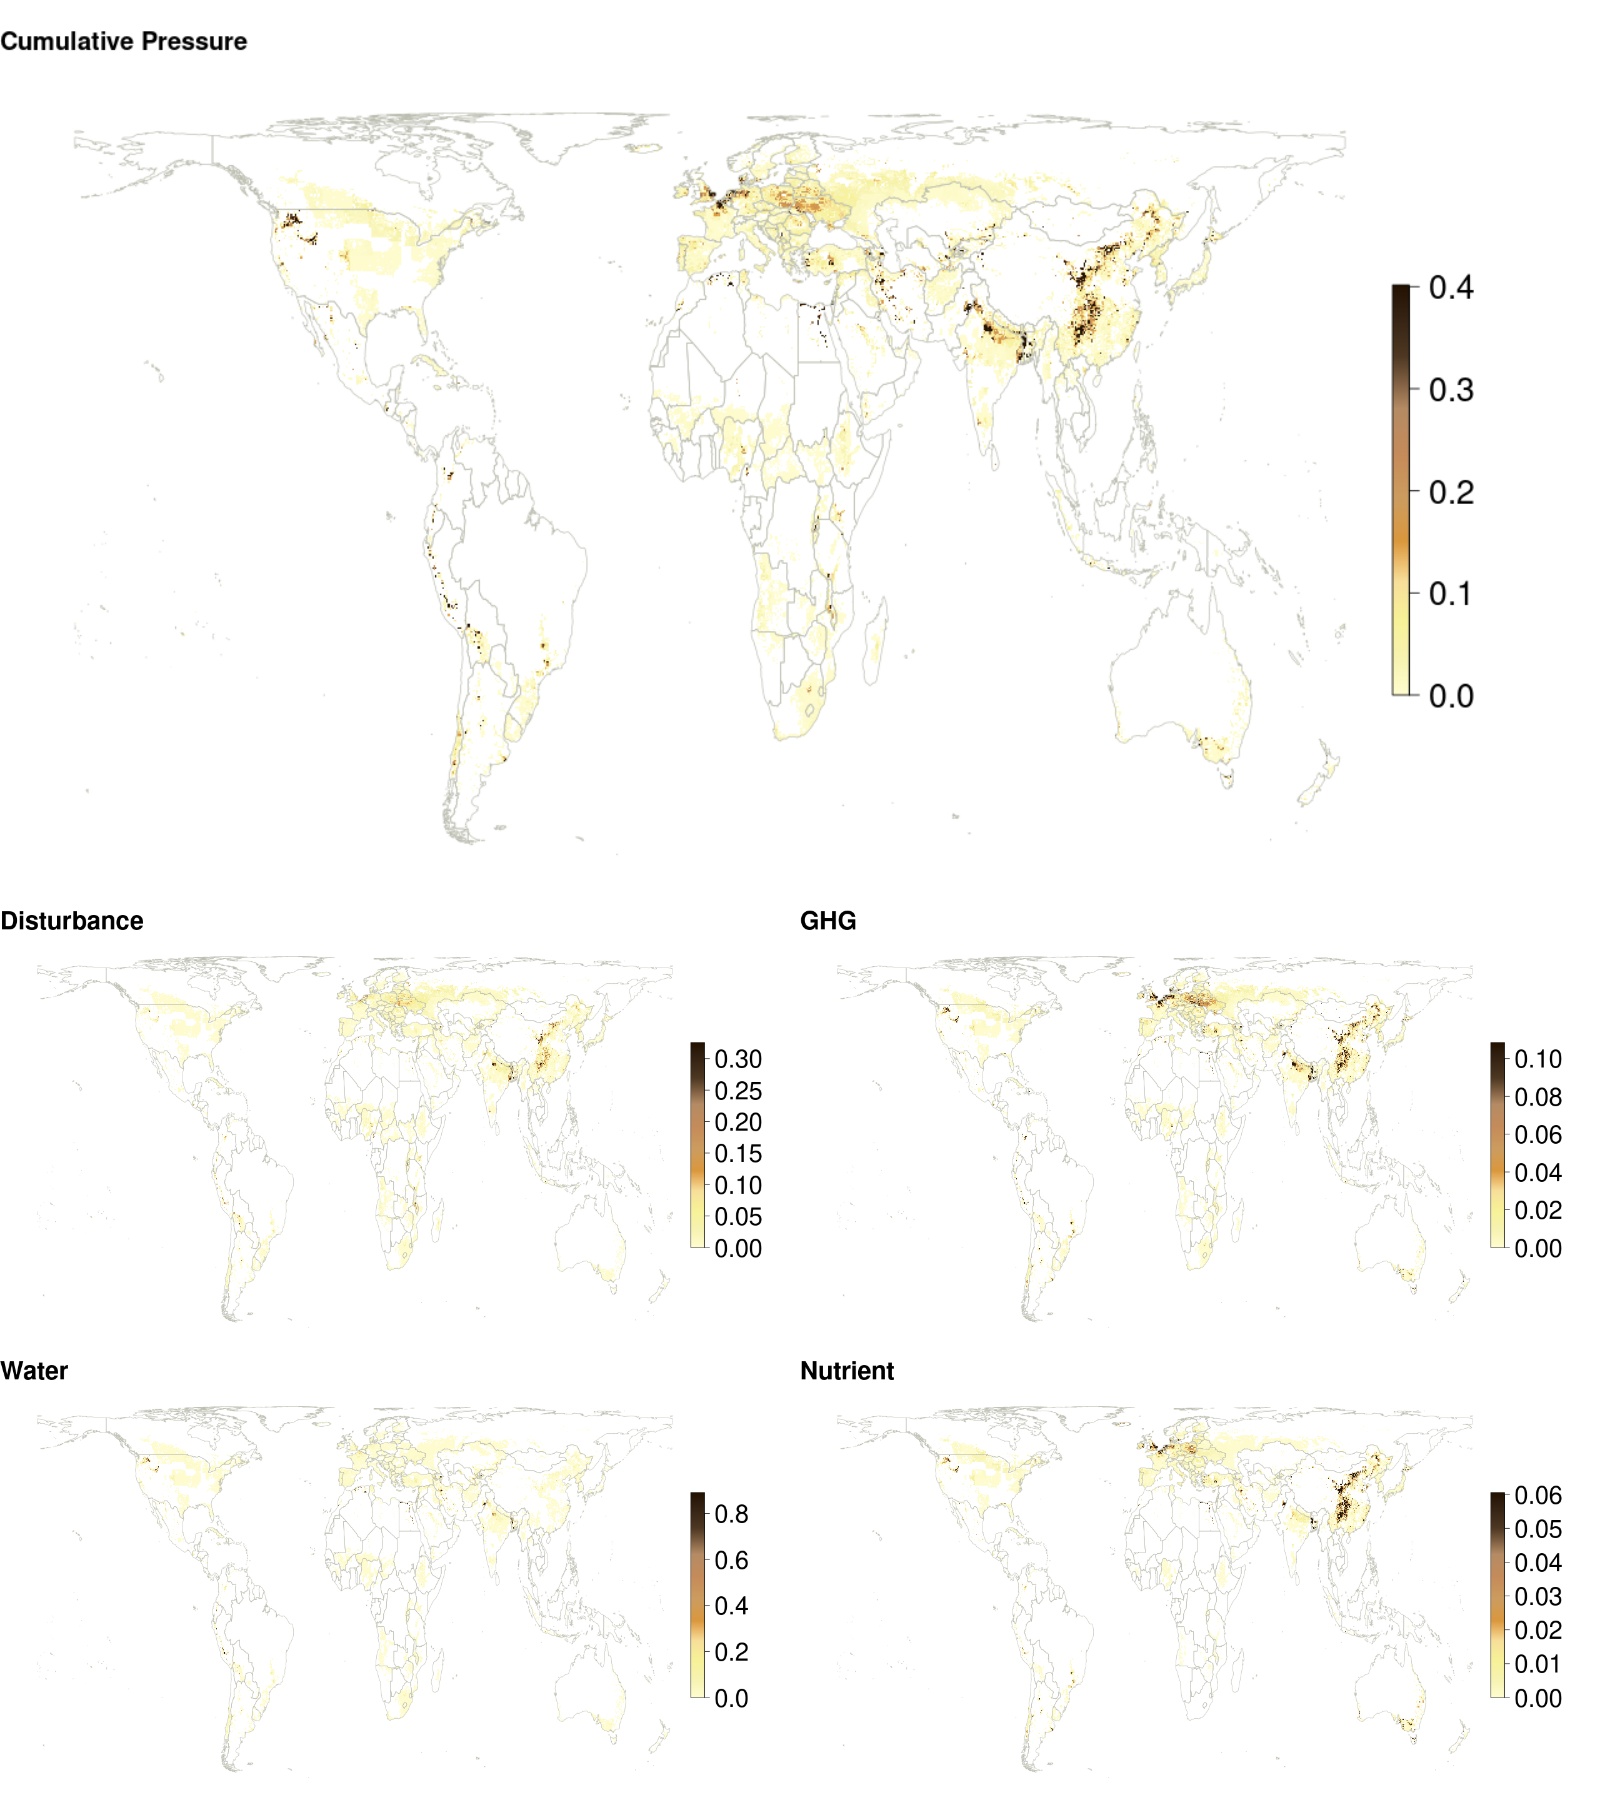
\includegraphics{/home/rayner/food-systems/_analysis/figures/extended_data/output/ed_fig_1_png/pota_crop_final.png}

\begin{center}\rule{0.5\linewidth}{0.5pt}\end{center}

\hypertarget{rice}{%
\subparagraph{13) Rice}\label{rice}}

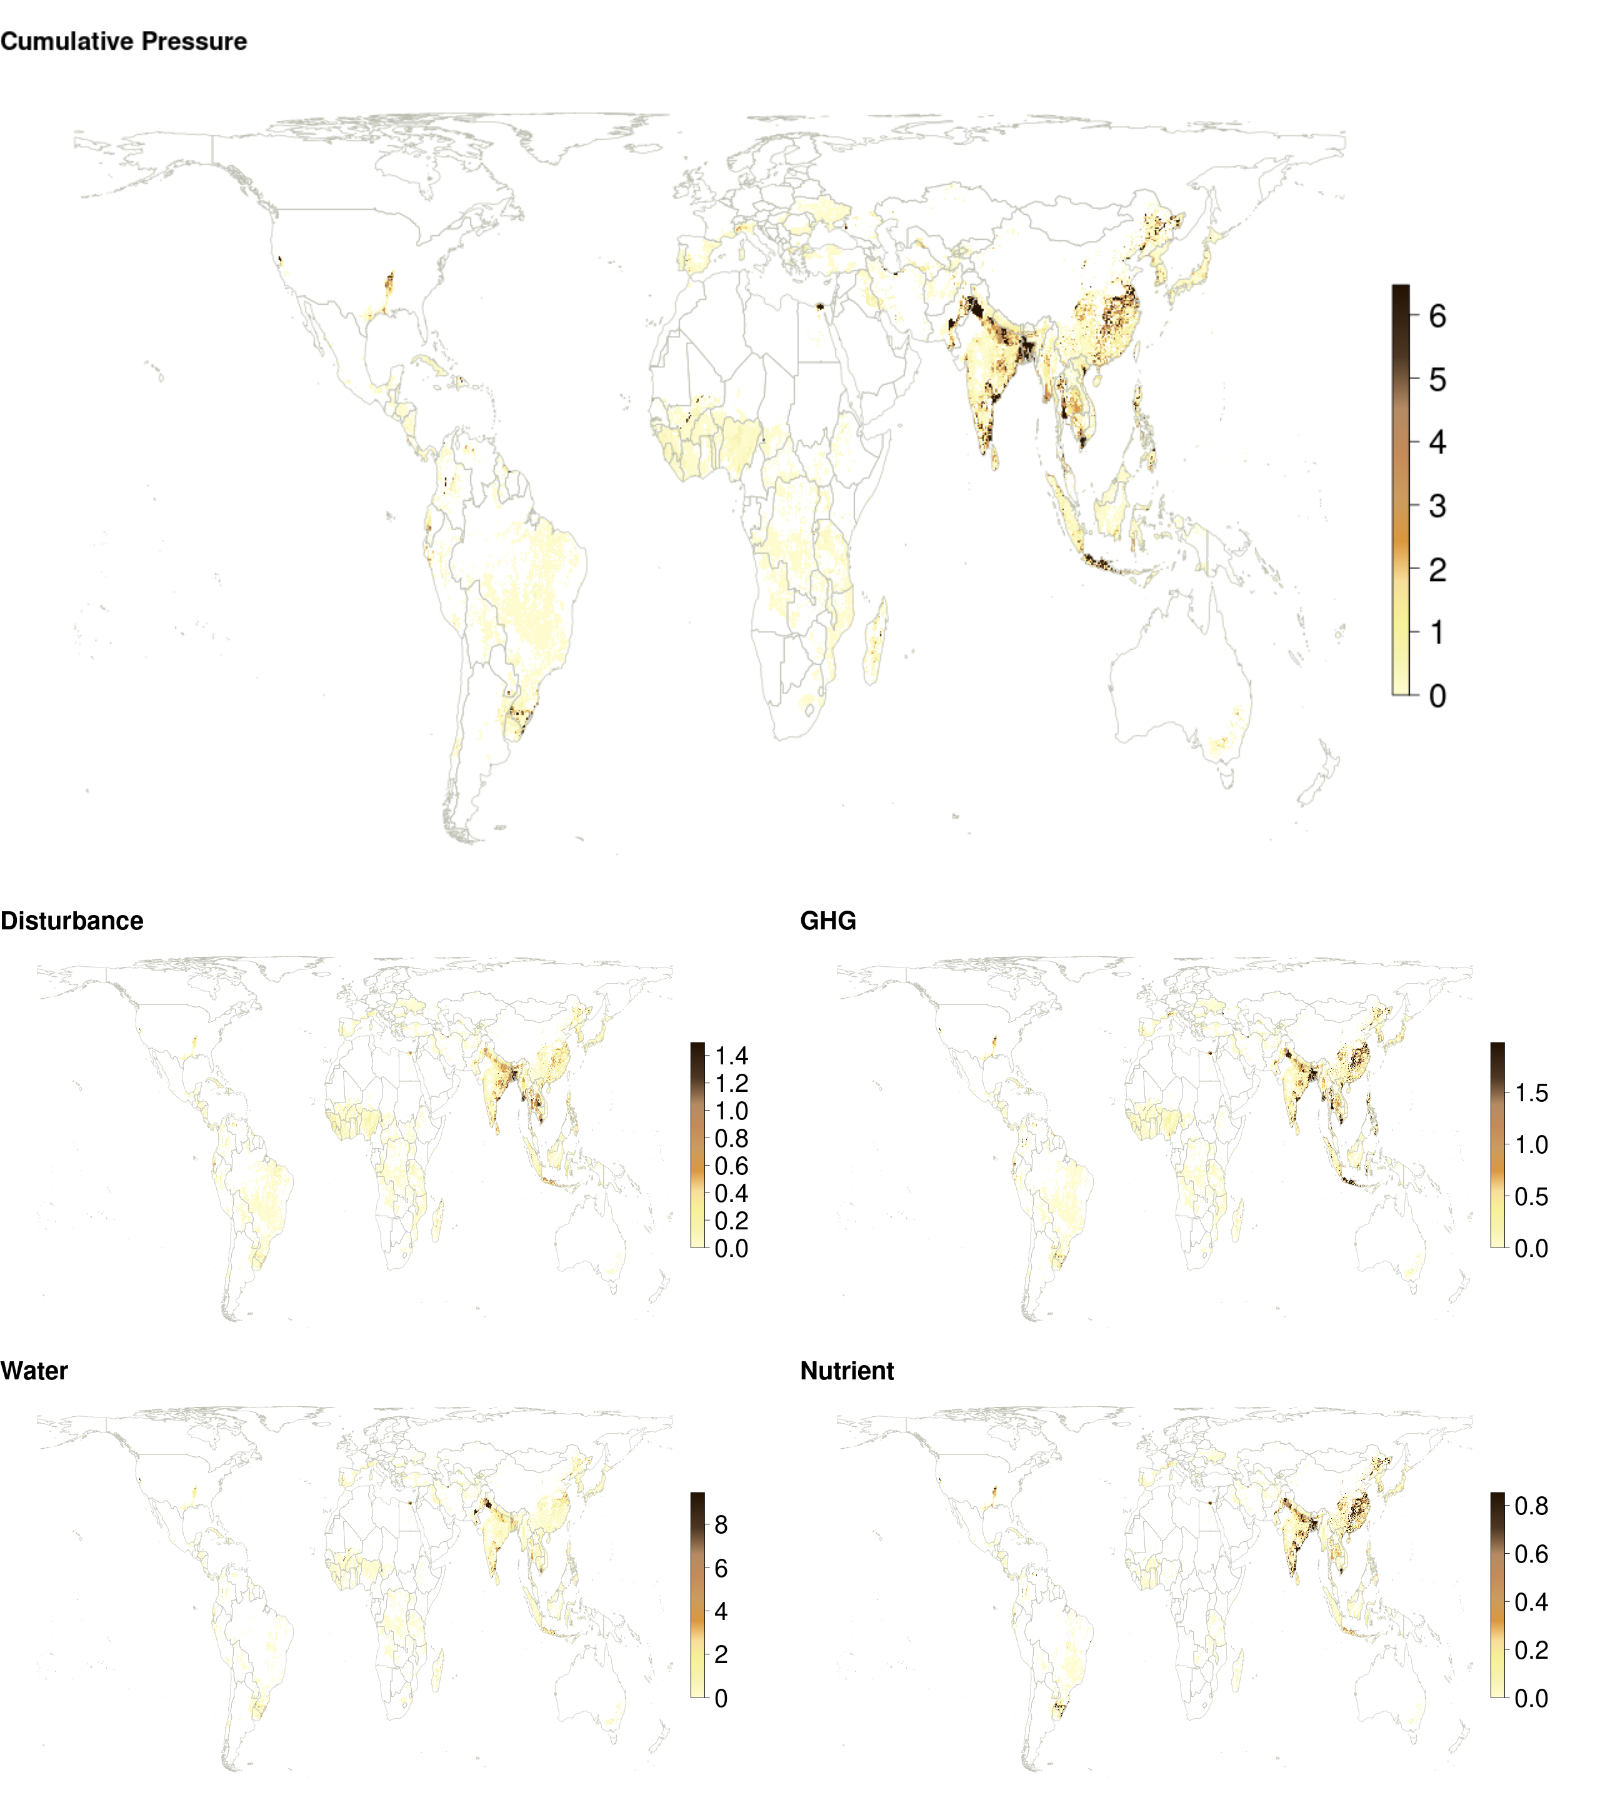
\includegraphics{/home/rayner/food-systems/_analysis/figures/extended_data/output/ed_fig_1_png/rice_crop_final.png}

\begin{center}\rule{0.5\linewidth}{0.5pt}\end{center}

\hypertarget{sorghum}{%
\subparagraph{14) Sorghum}\label{sorghum}}

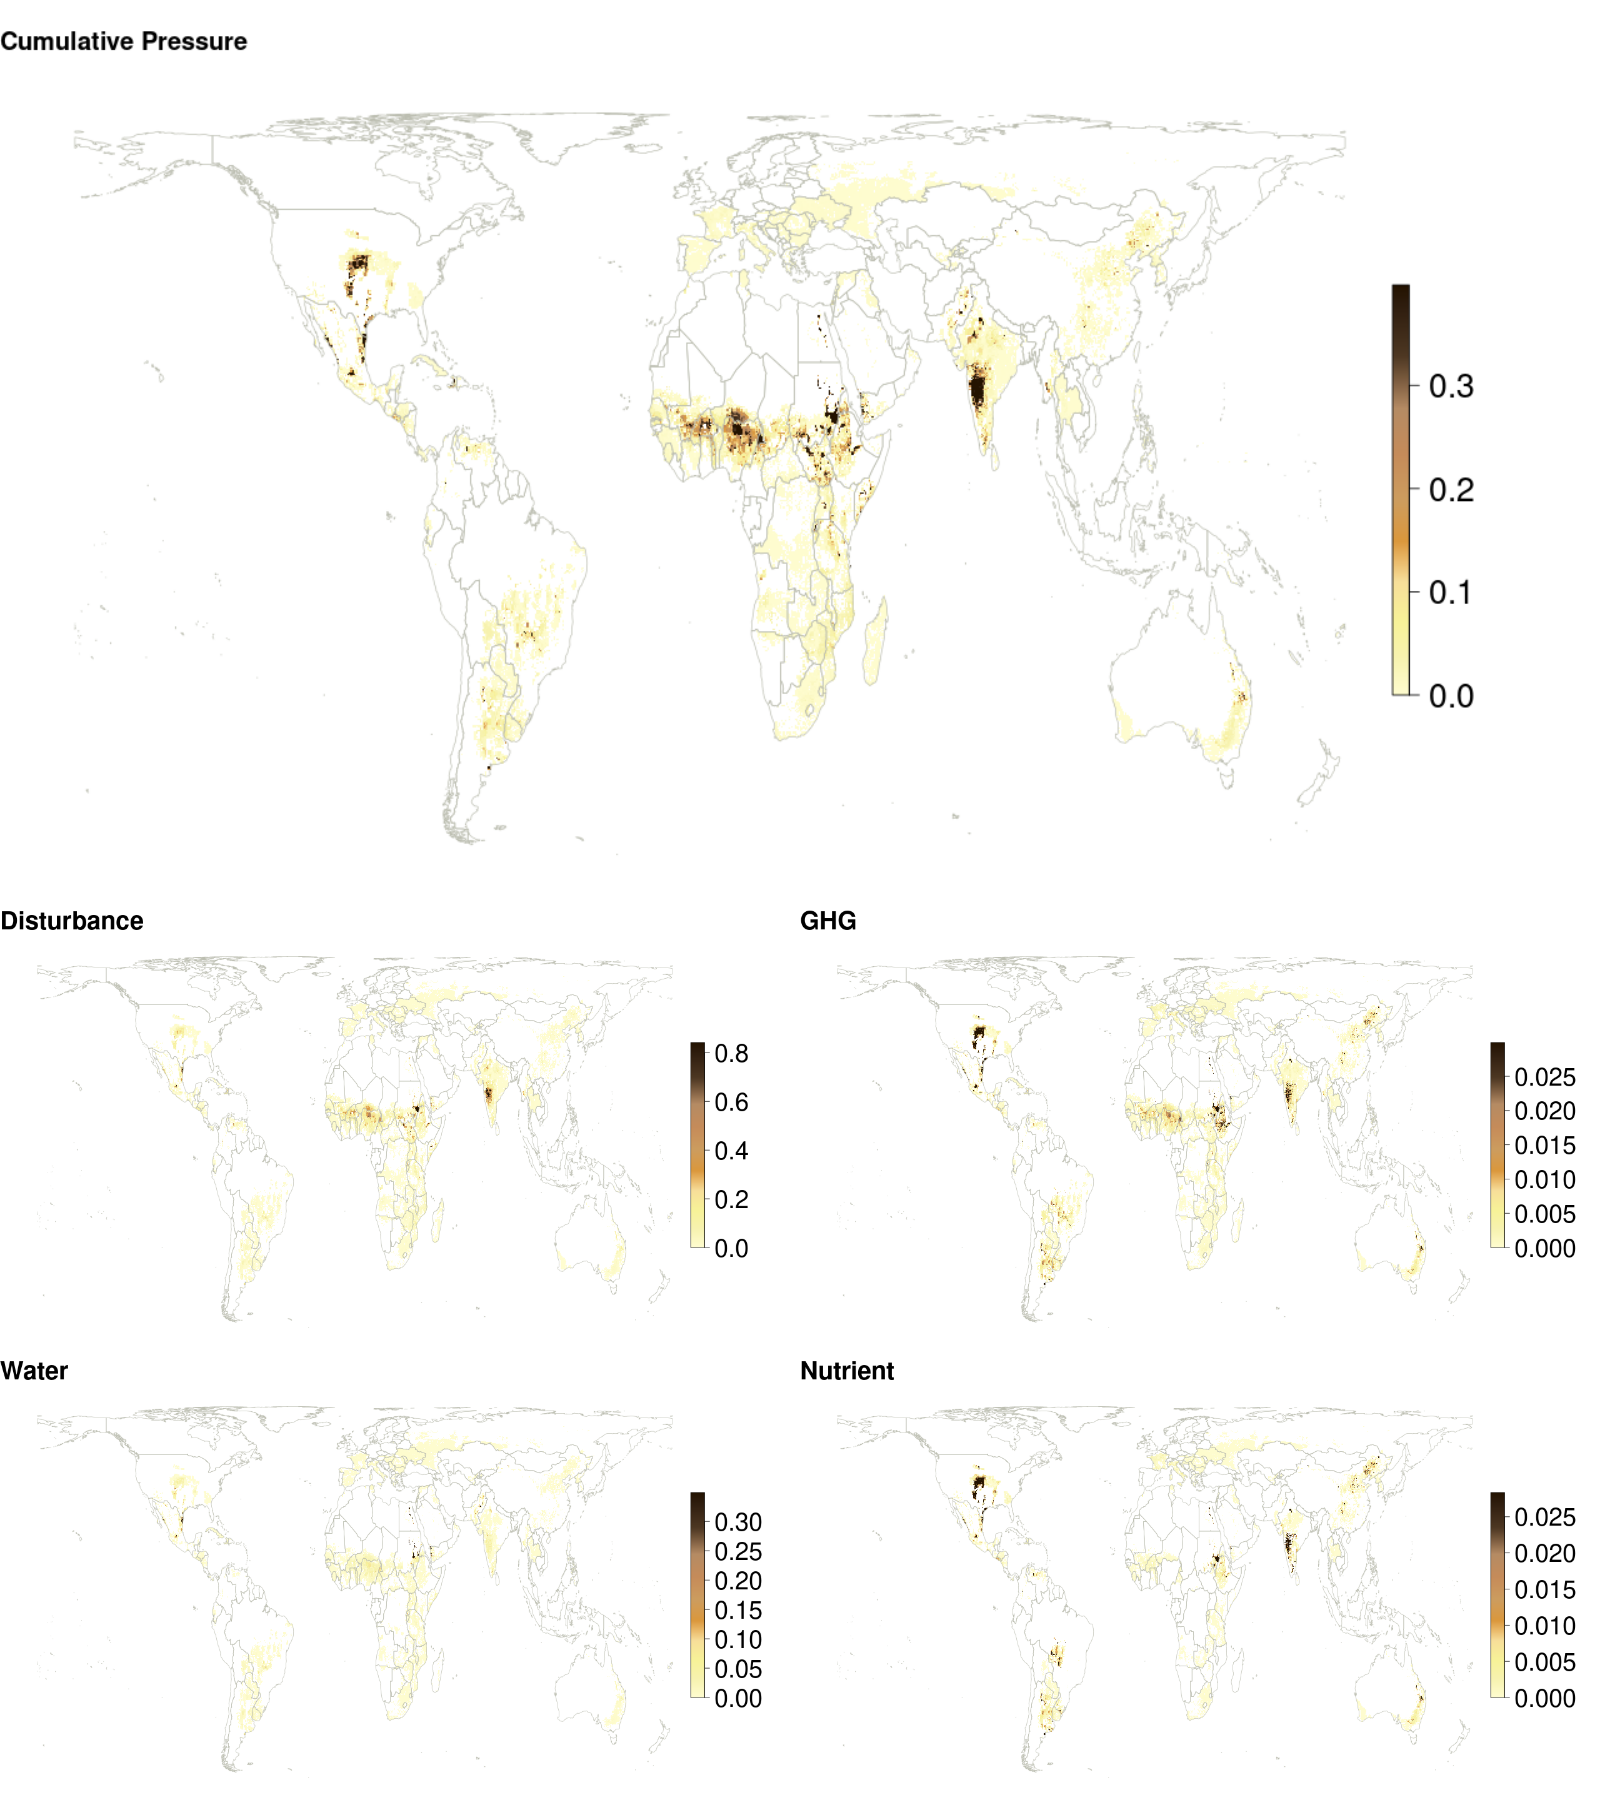
\includegraphics{/home/rayner/food-systems/_analysis/figures/extended_data/output/ed_fig_1_png/sorg_crop_final.png}

\begin{center}\rule{0.5\linewidth}{0.5pt}\end{center}

\hypertarget{soybean}{%
\subparagraph{15) Soybean}\label{soybean}}

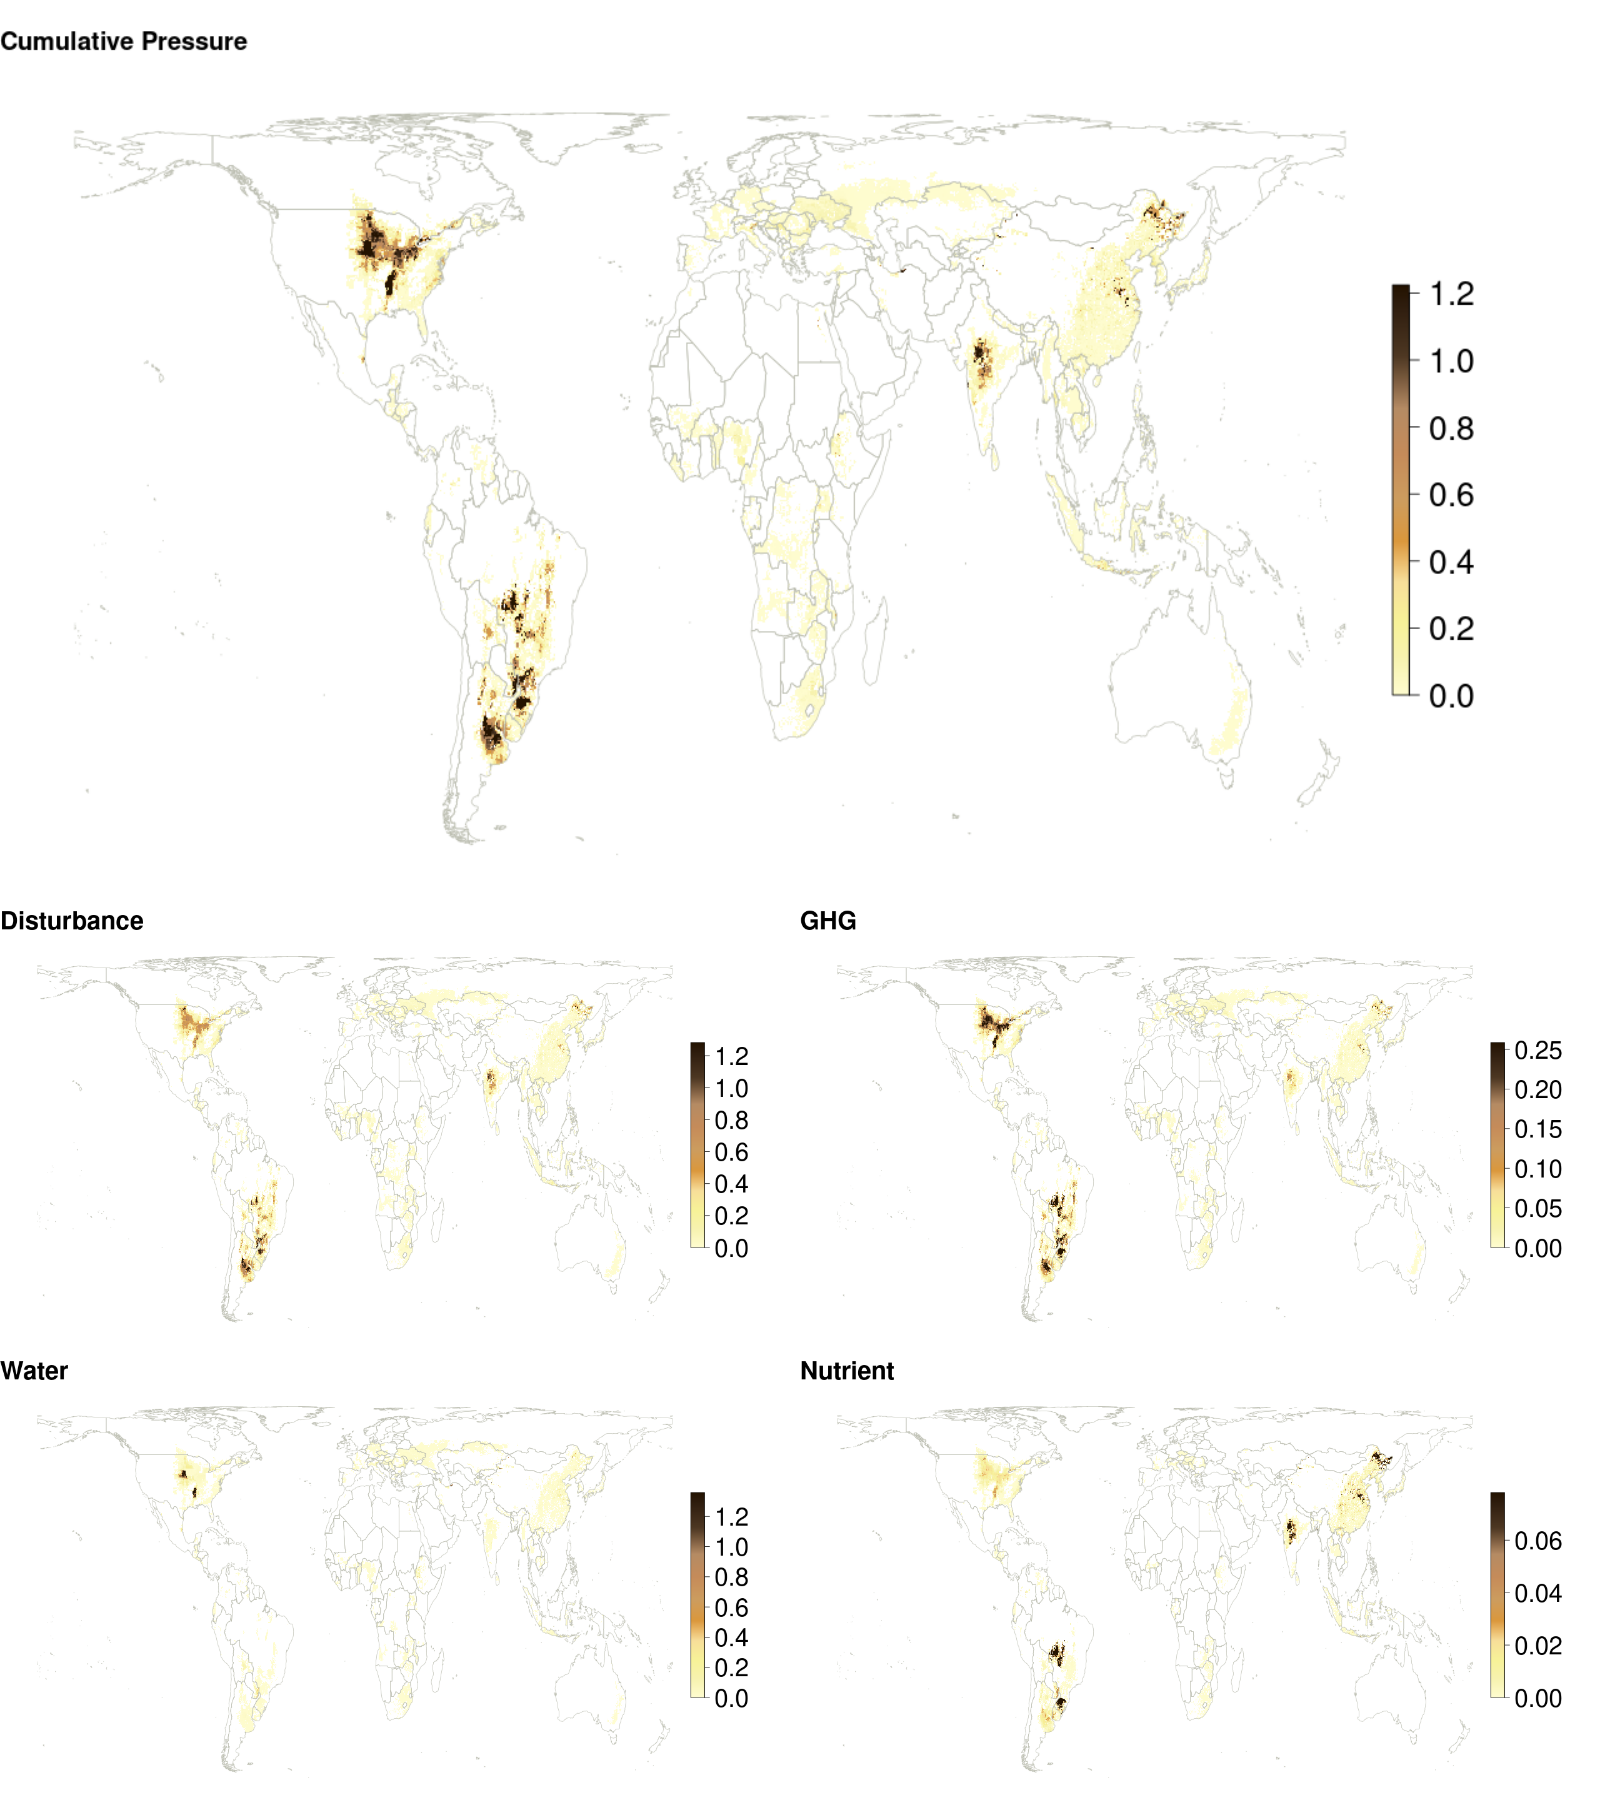
\includegraphics{/home/rayner/food-systems/_analysis/figures/extended_data/output/ed_fig_1_png/soyb_crop_final.png}

\begin{center}\rule{0.5\linewidth}{0.5pt}\end{center}

\hypertarget{spices}{%
\subparagraph{16) Spices}\label{spices}}

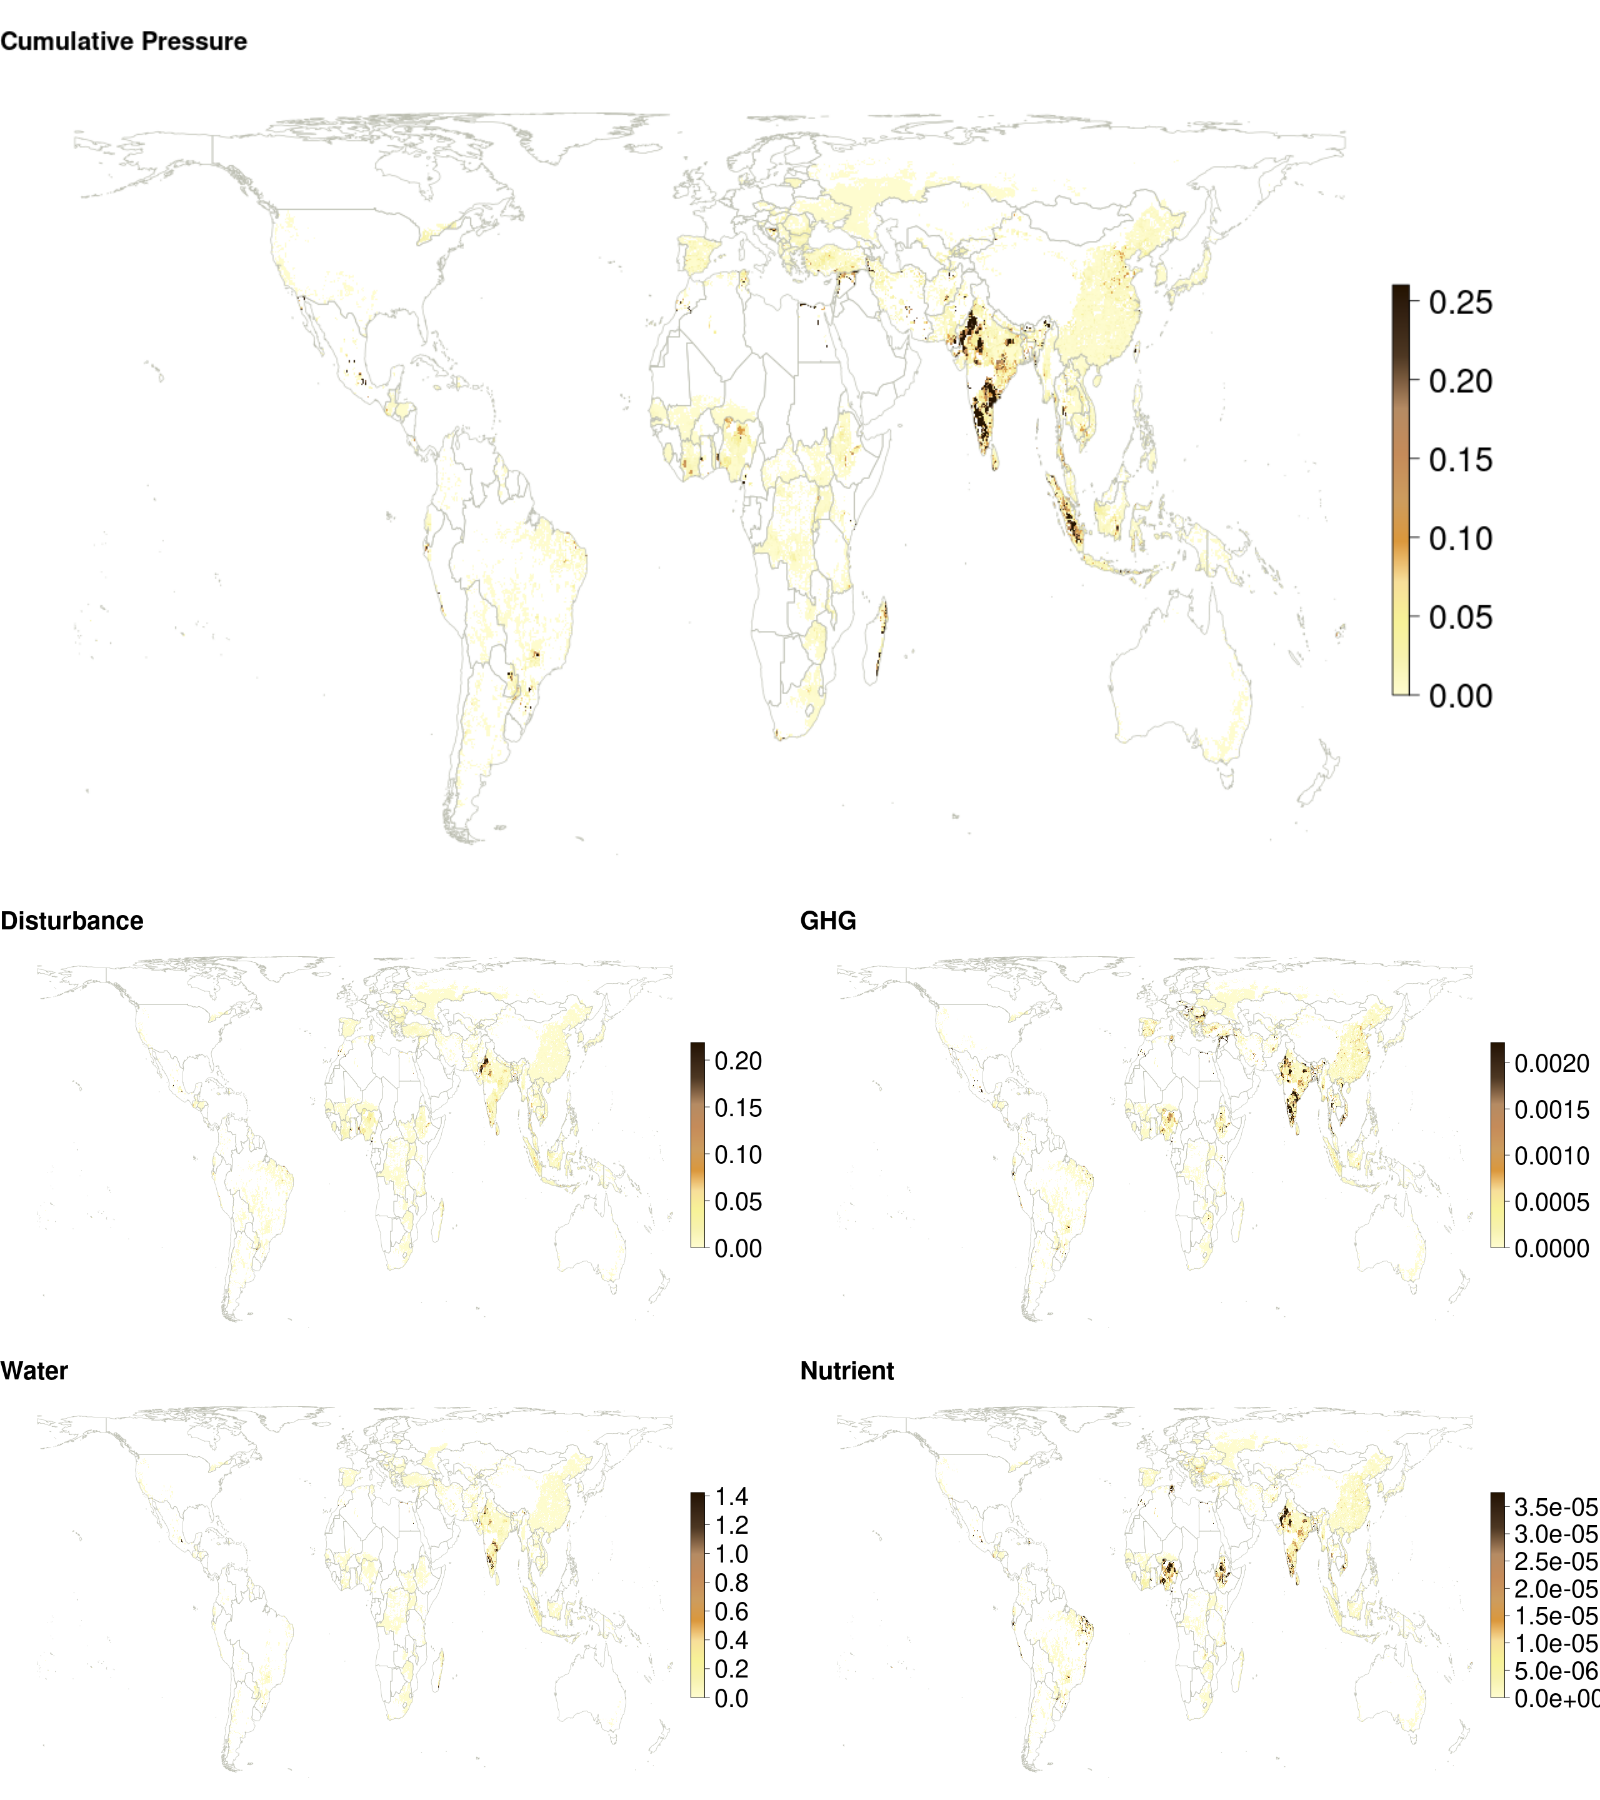
\includegraphics{/home/rayner/food-systems/_analysis/figures/extended_data/output/ed_fig_1_png/spis_crop_final.png}

\begin{center}\rule{0.5\linewidth}{0.5pt}\end{center}

\hypertarget{sugarbeet}{%
\subparagraph{17) Sugarbeet}\label{sugarbeet}}

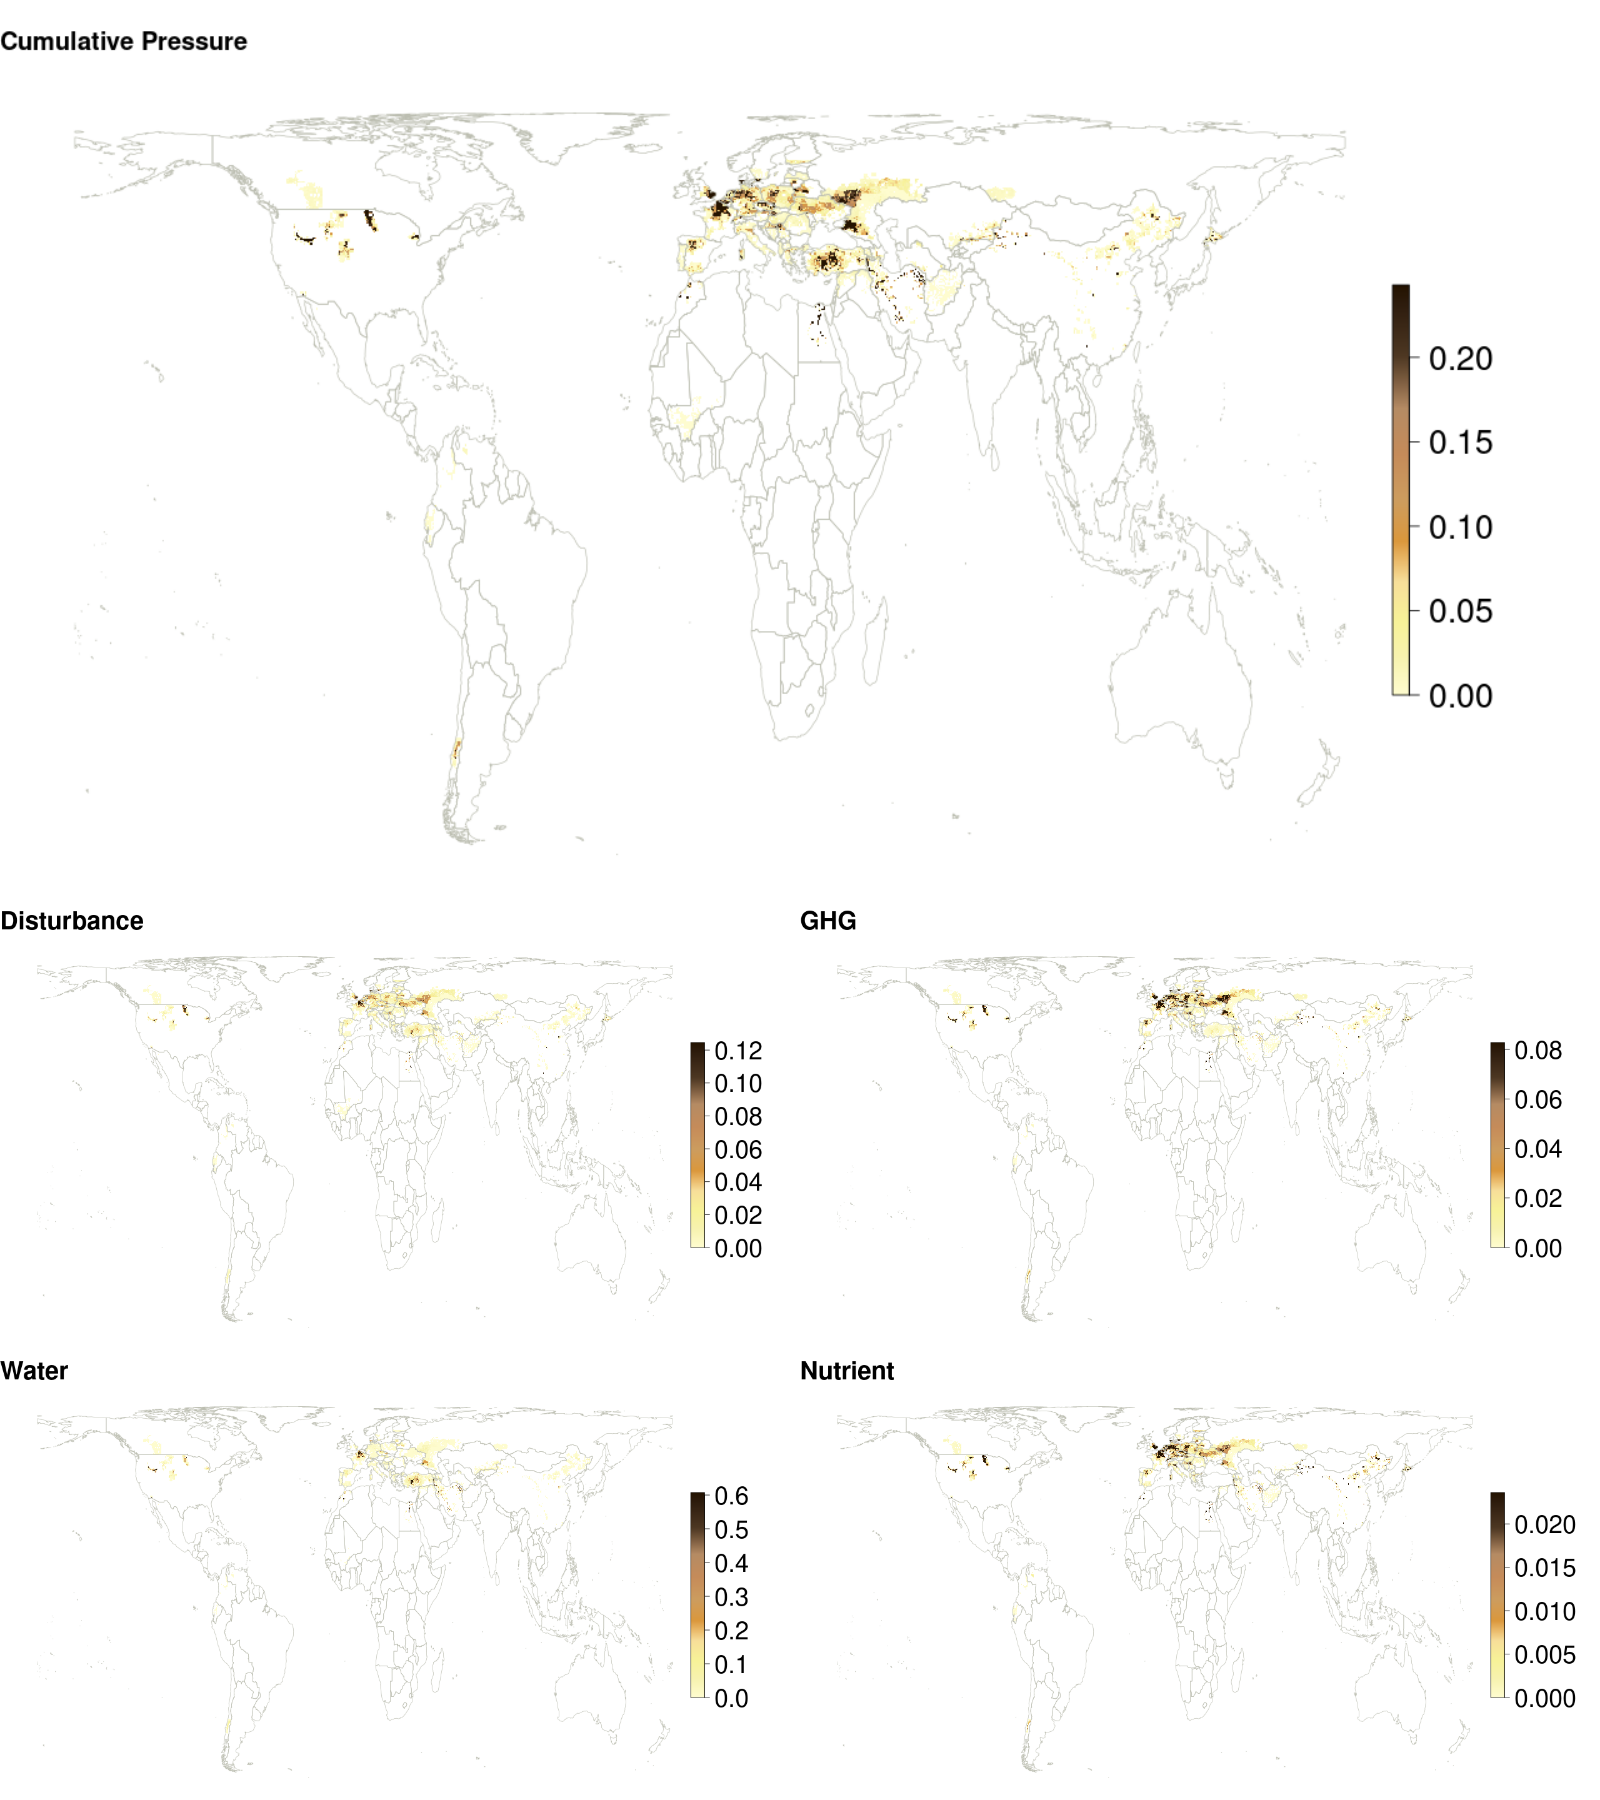
\includegraphics{/home/rayner/food-systems/_analysis/figures/extended_data/output/ed_fig_1_png/sugb_crop_final.png}

\begin{center}\rule{0.5\linewidth}{0.5pt}\end{center}

\hypertarget{sugarcane}{%
\subparagraph{18) Sugarcane}\label{sugarcane}}

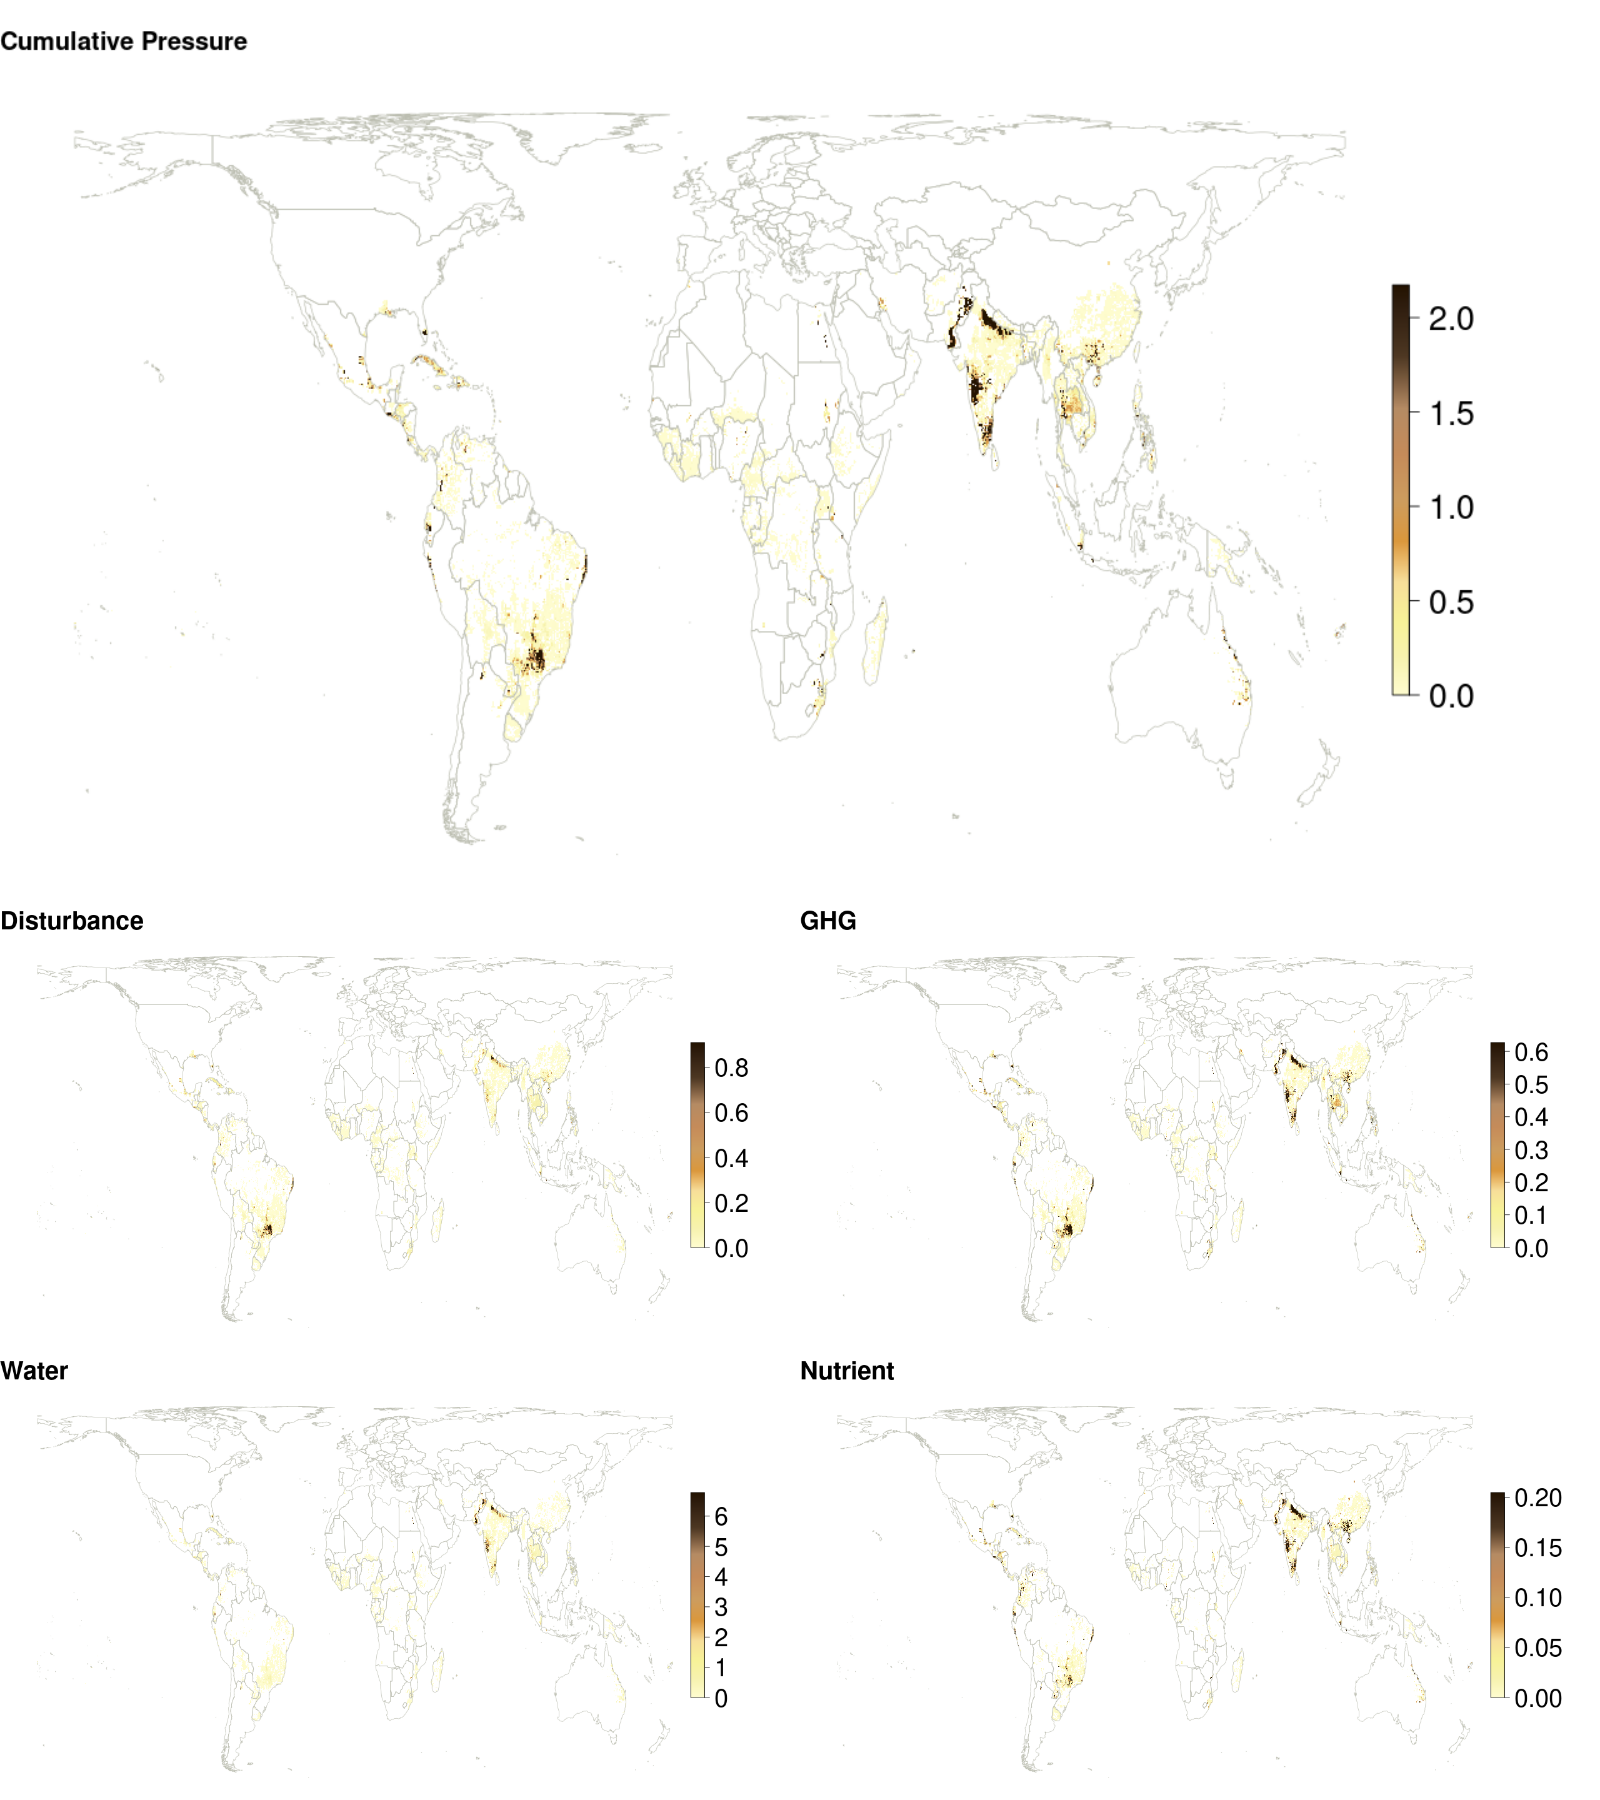
\includegraphics{/home/rayner/food-systems/_analysis/figures/extended_data/output/ed_fig_1_png/sugc_crop_final.png}

\begin{center}\rule{0.5\linewidth}{0.5pt}\end{center}

\hypertarget{sweet-potato}{%
\subparagraph{19) Sweet potato}\label{sweet-potato}}

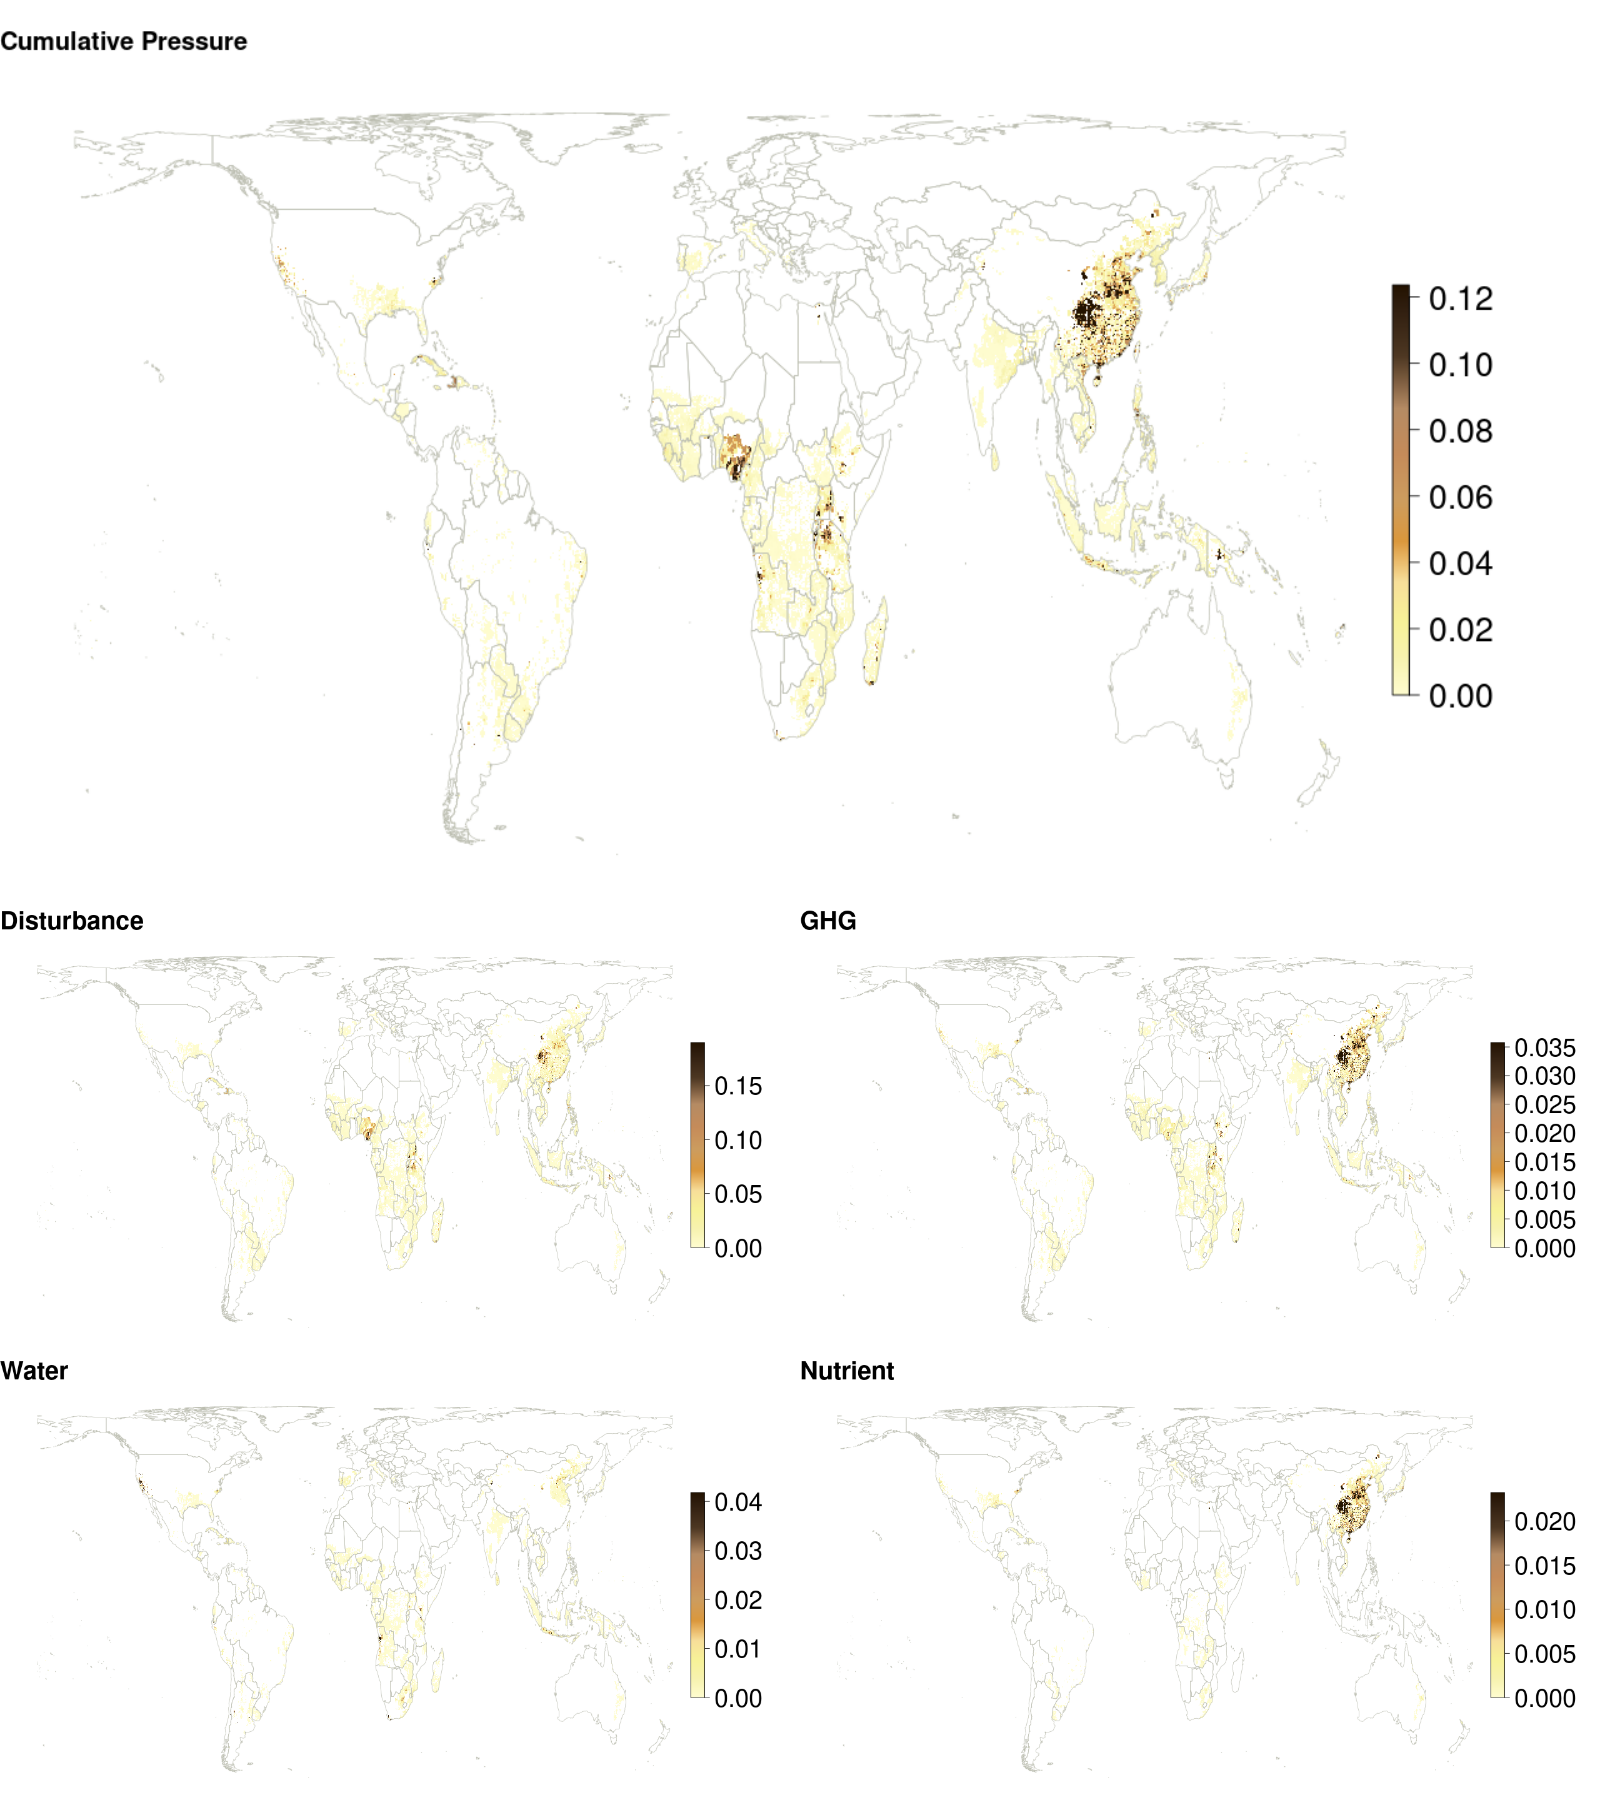
\includegraphics{/home/rayner/food-systems/_analysis/figures/extended_data/output/ed_fig_1_png/swpo_crop_final.png}

\begin{center}\rule{0.5\linewidth}{0.5pt}\end{center}

\hypertarget{treenuts}{%
\subparagraph{20) Treenuts}\label{treenuts}}

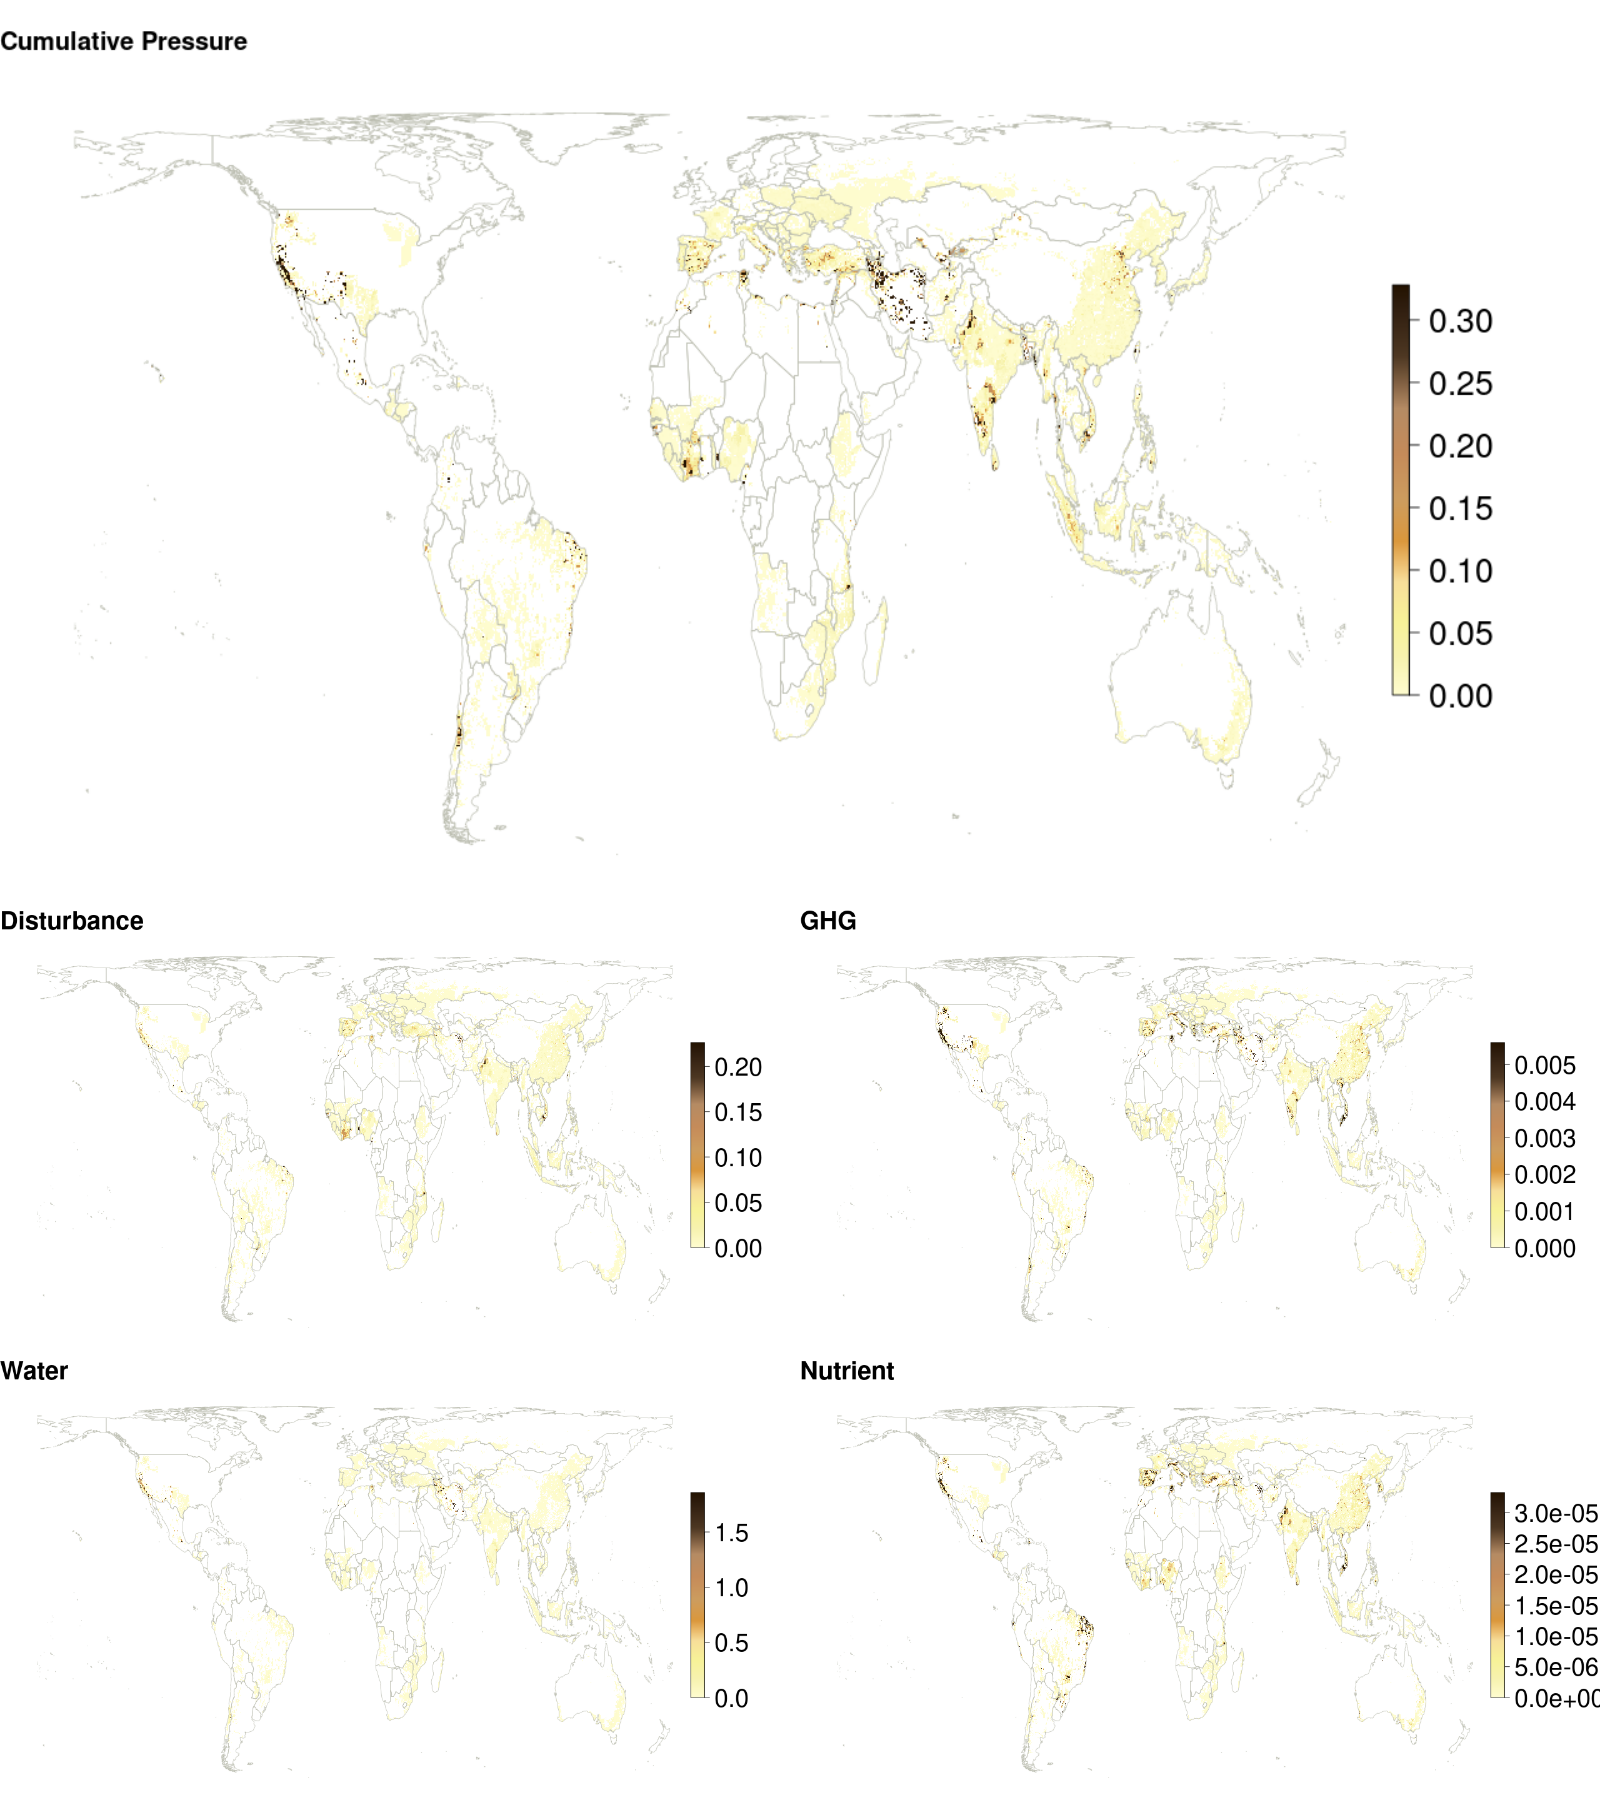
\includegraphics{/home/rayner/food-systems/_analysis/figures/extended_data/output/ed_fig_1_png/tnut_crop_final.png}

\begin{center}\rule{0.5\linewidth}{0.5pt}\end{center}

\hypertarget{vegetables}{%
\subparagraph{21) Vegetables}\label{vegetables}}

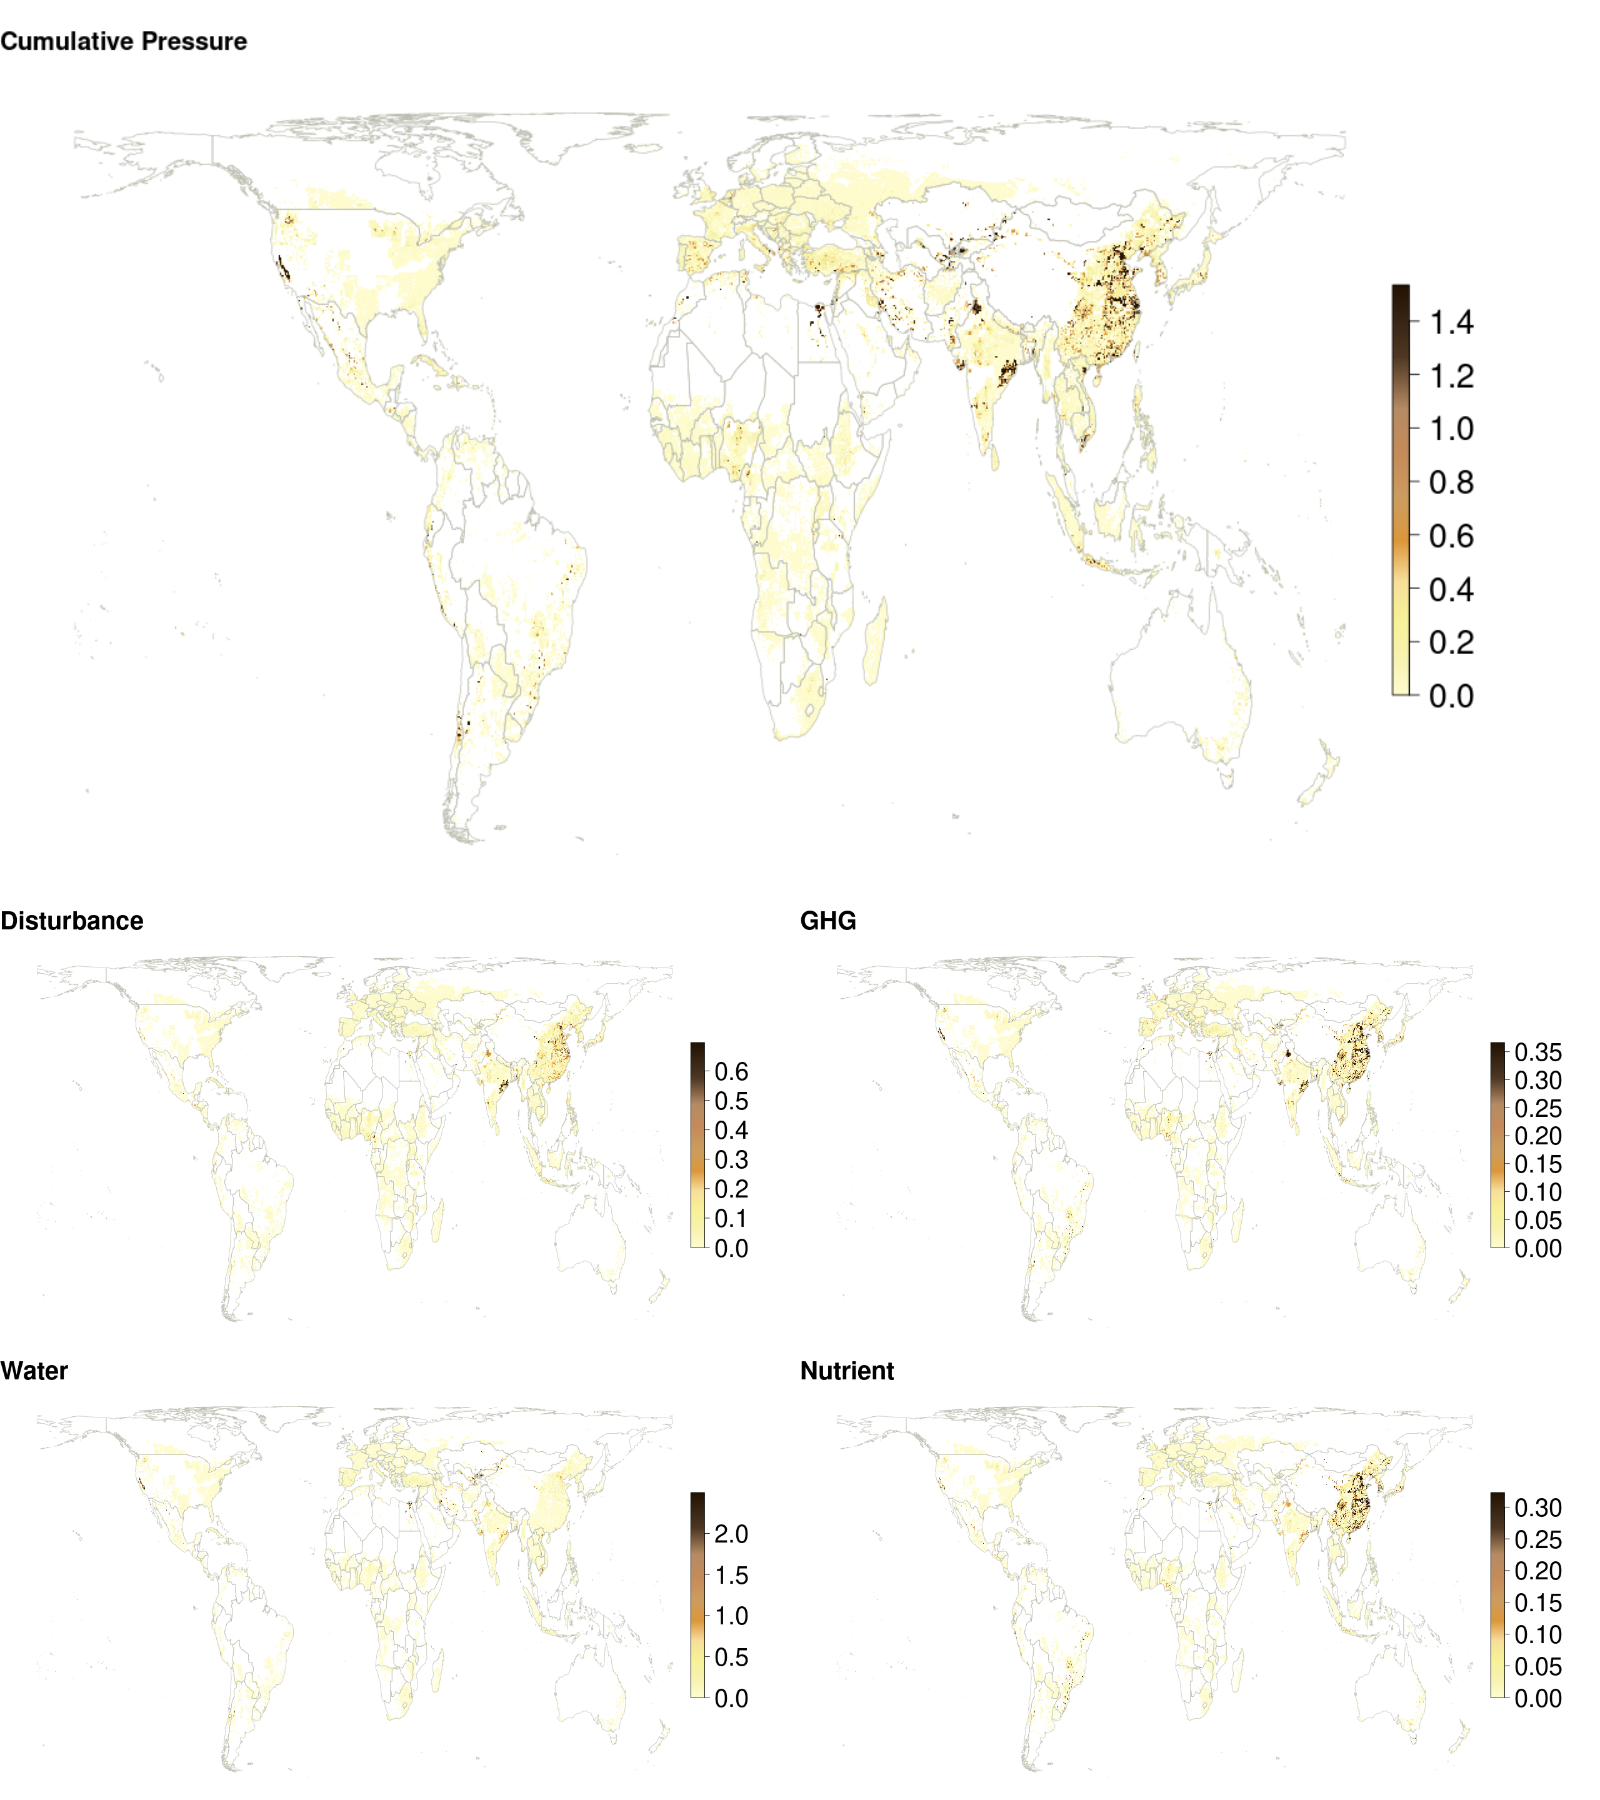
\includegraphics{/home/rayner/food-systems/_analysis/figures/extended_data/output/ed_fig_1_png/vege_crop_final.png}

\begin{center}\rule{0.5\linewidth}{0.5pt}\end{center}

\hypertarget{wheat}{%
\subparagraph{22) Wheat}\label{wheat}}

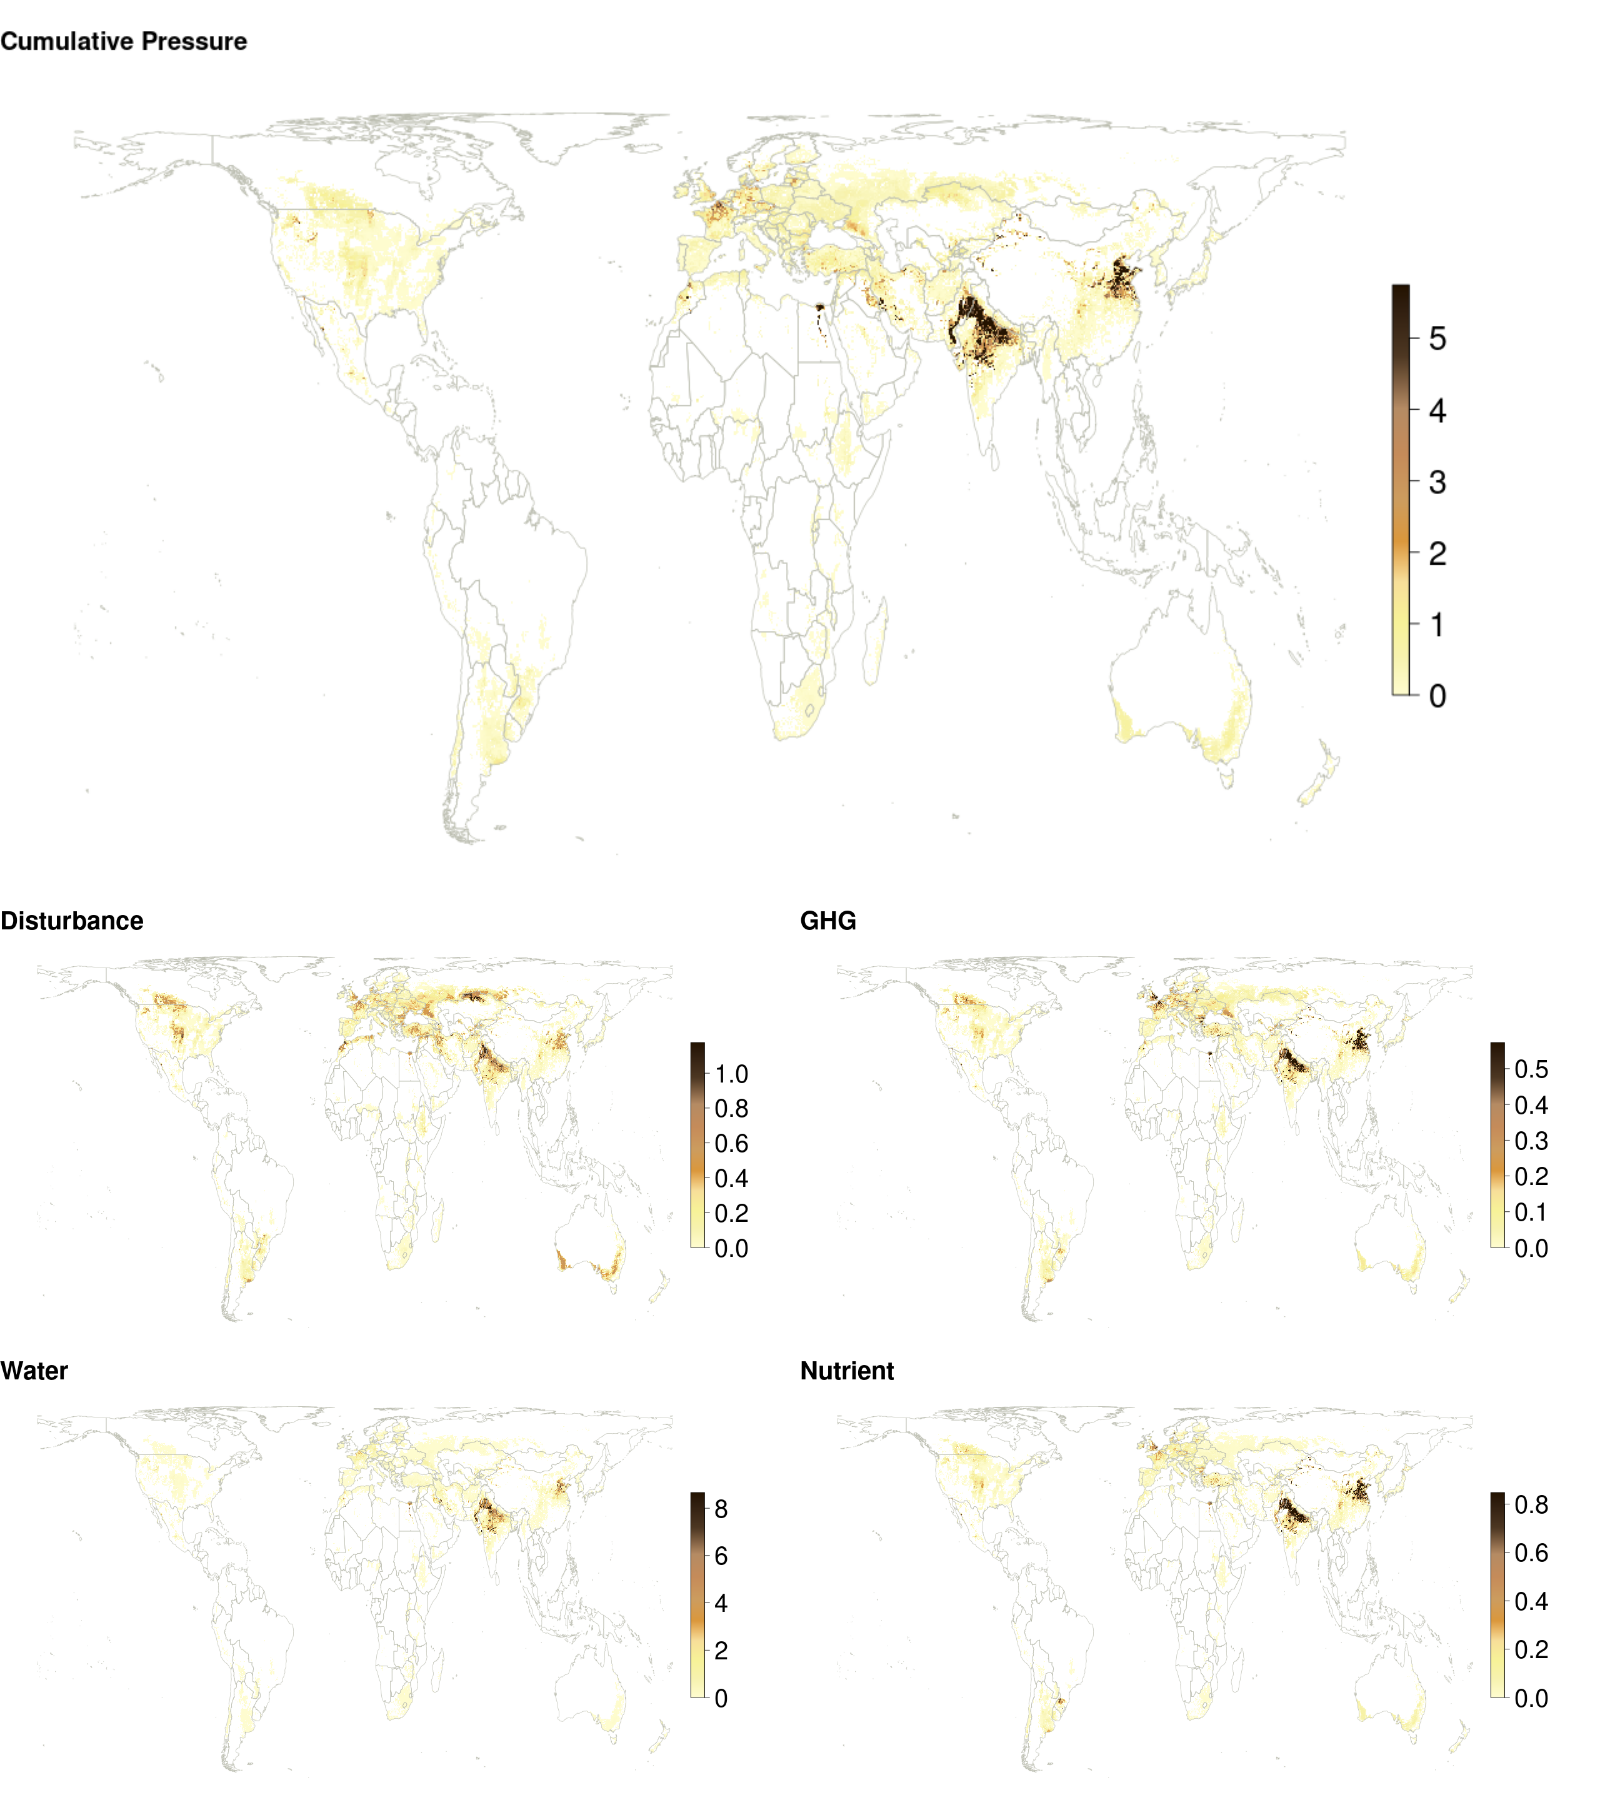
\includegraphics{/home/rayner/food-systems/_analysis/figures/extended_data/output/ed_fig_1_png/whea_crop_final.png}

\begin{center}\rule{0.5\linewidth}{0.5pt}\end{center}

\hypertarget{fruits}{%
\subparagraph{23) Fruits}\label{fruits}}

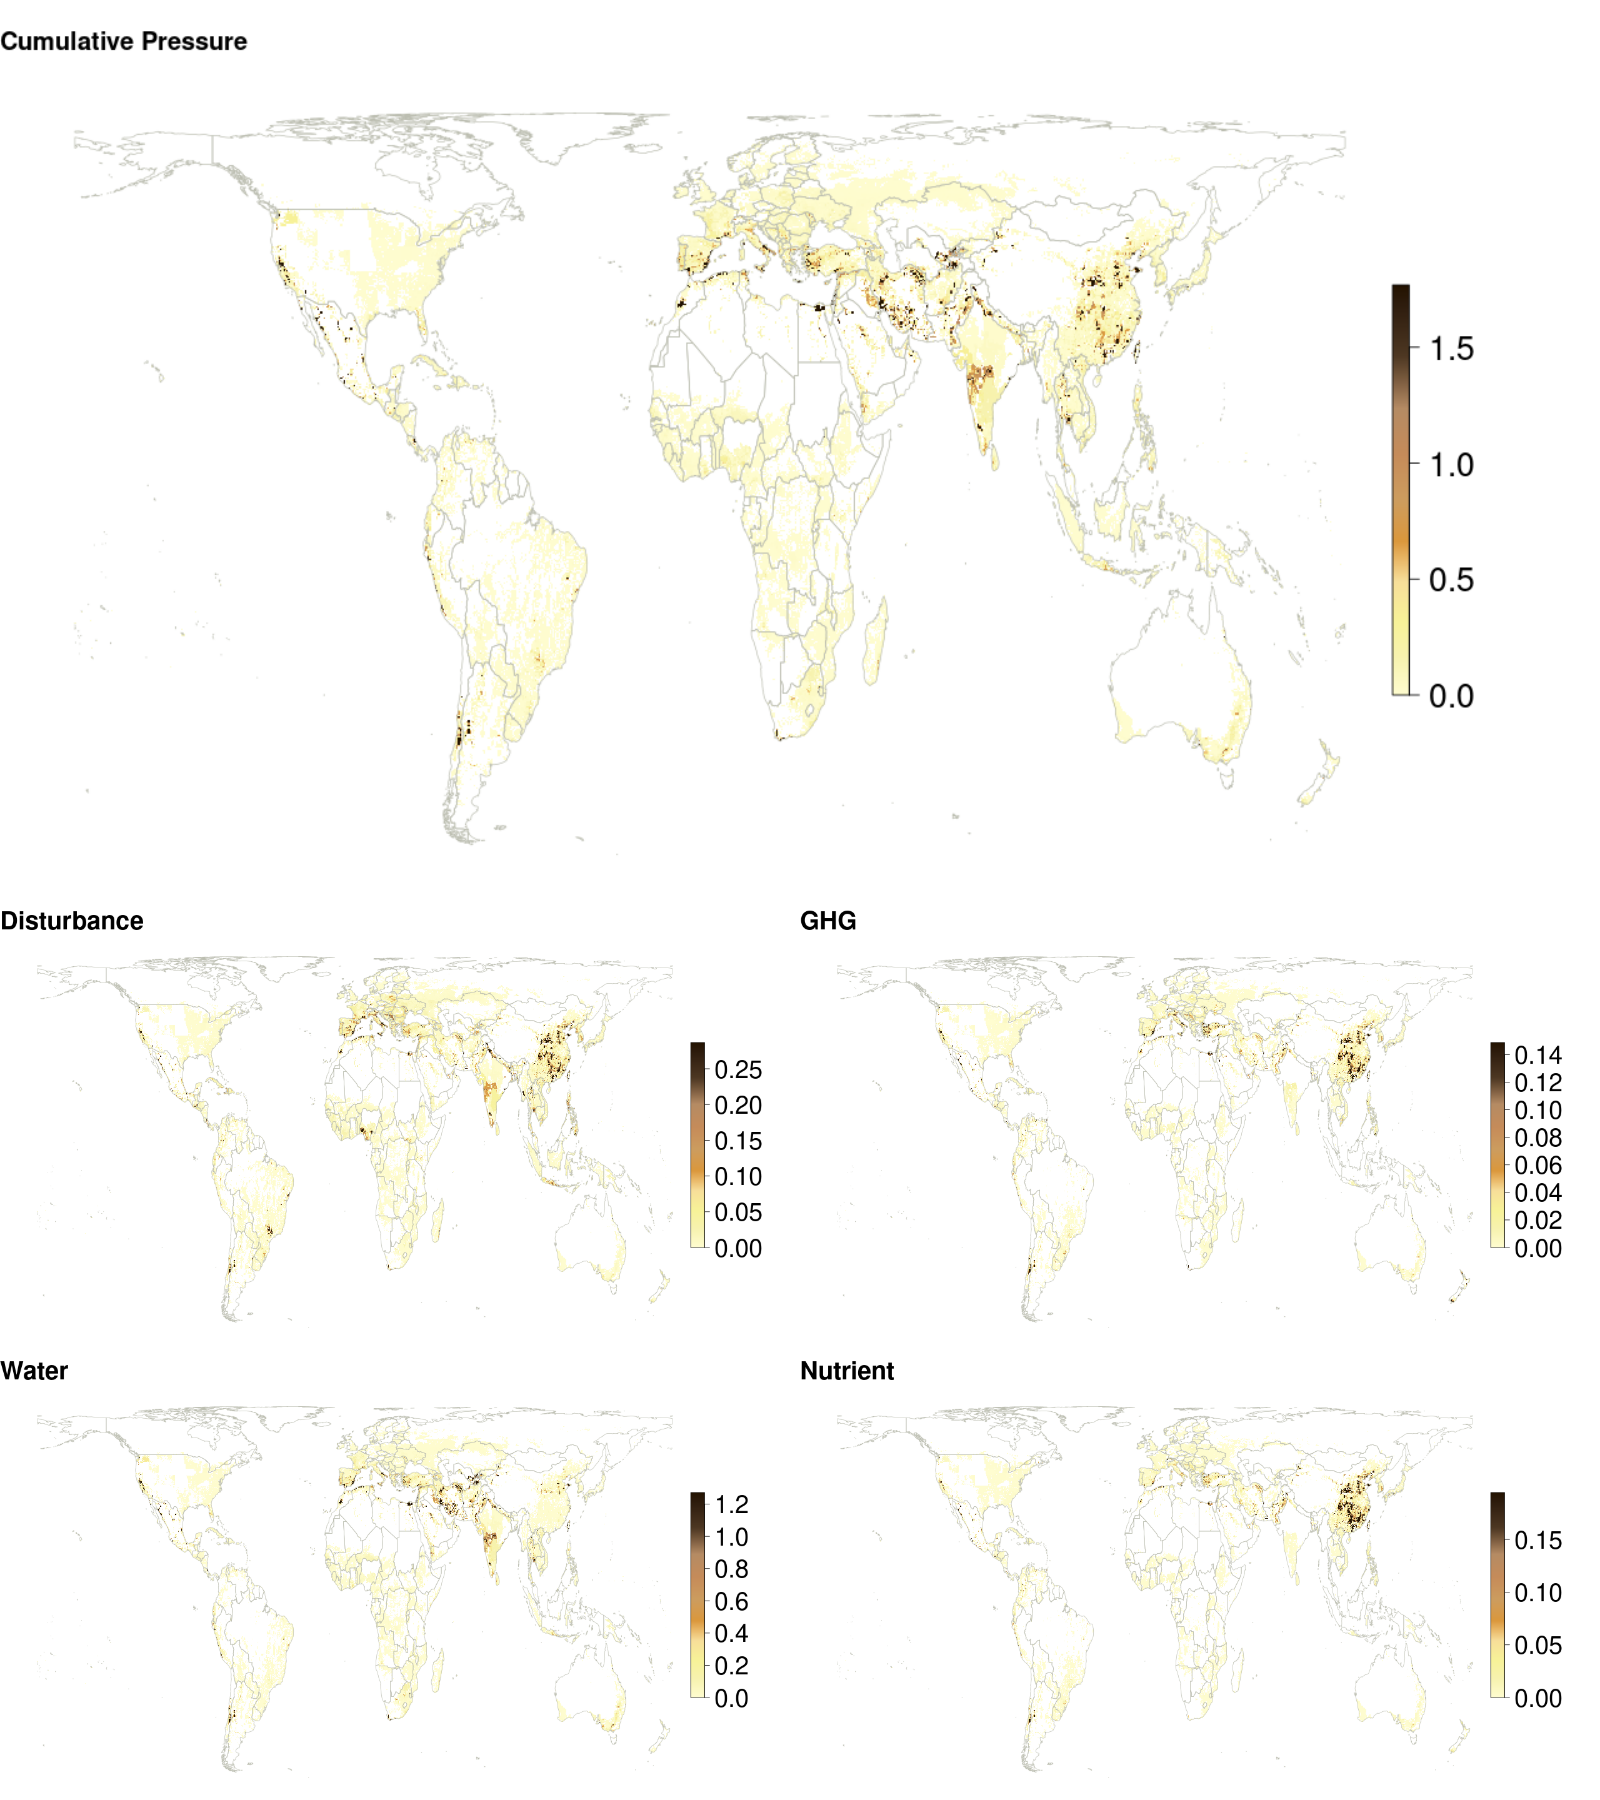
\includegraphics{/home/rayner/food-systems/_analysis/figures/extended_data/output/ed_fig_1_png/xfru_crop_final.png}

\begin{center}\rule{0.5\linewidth}{0.5pt}\end{center}

\hypertarget{millet}{%
\subparagraph{24) Millet}\label{millet}}

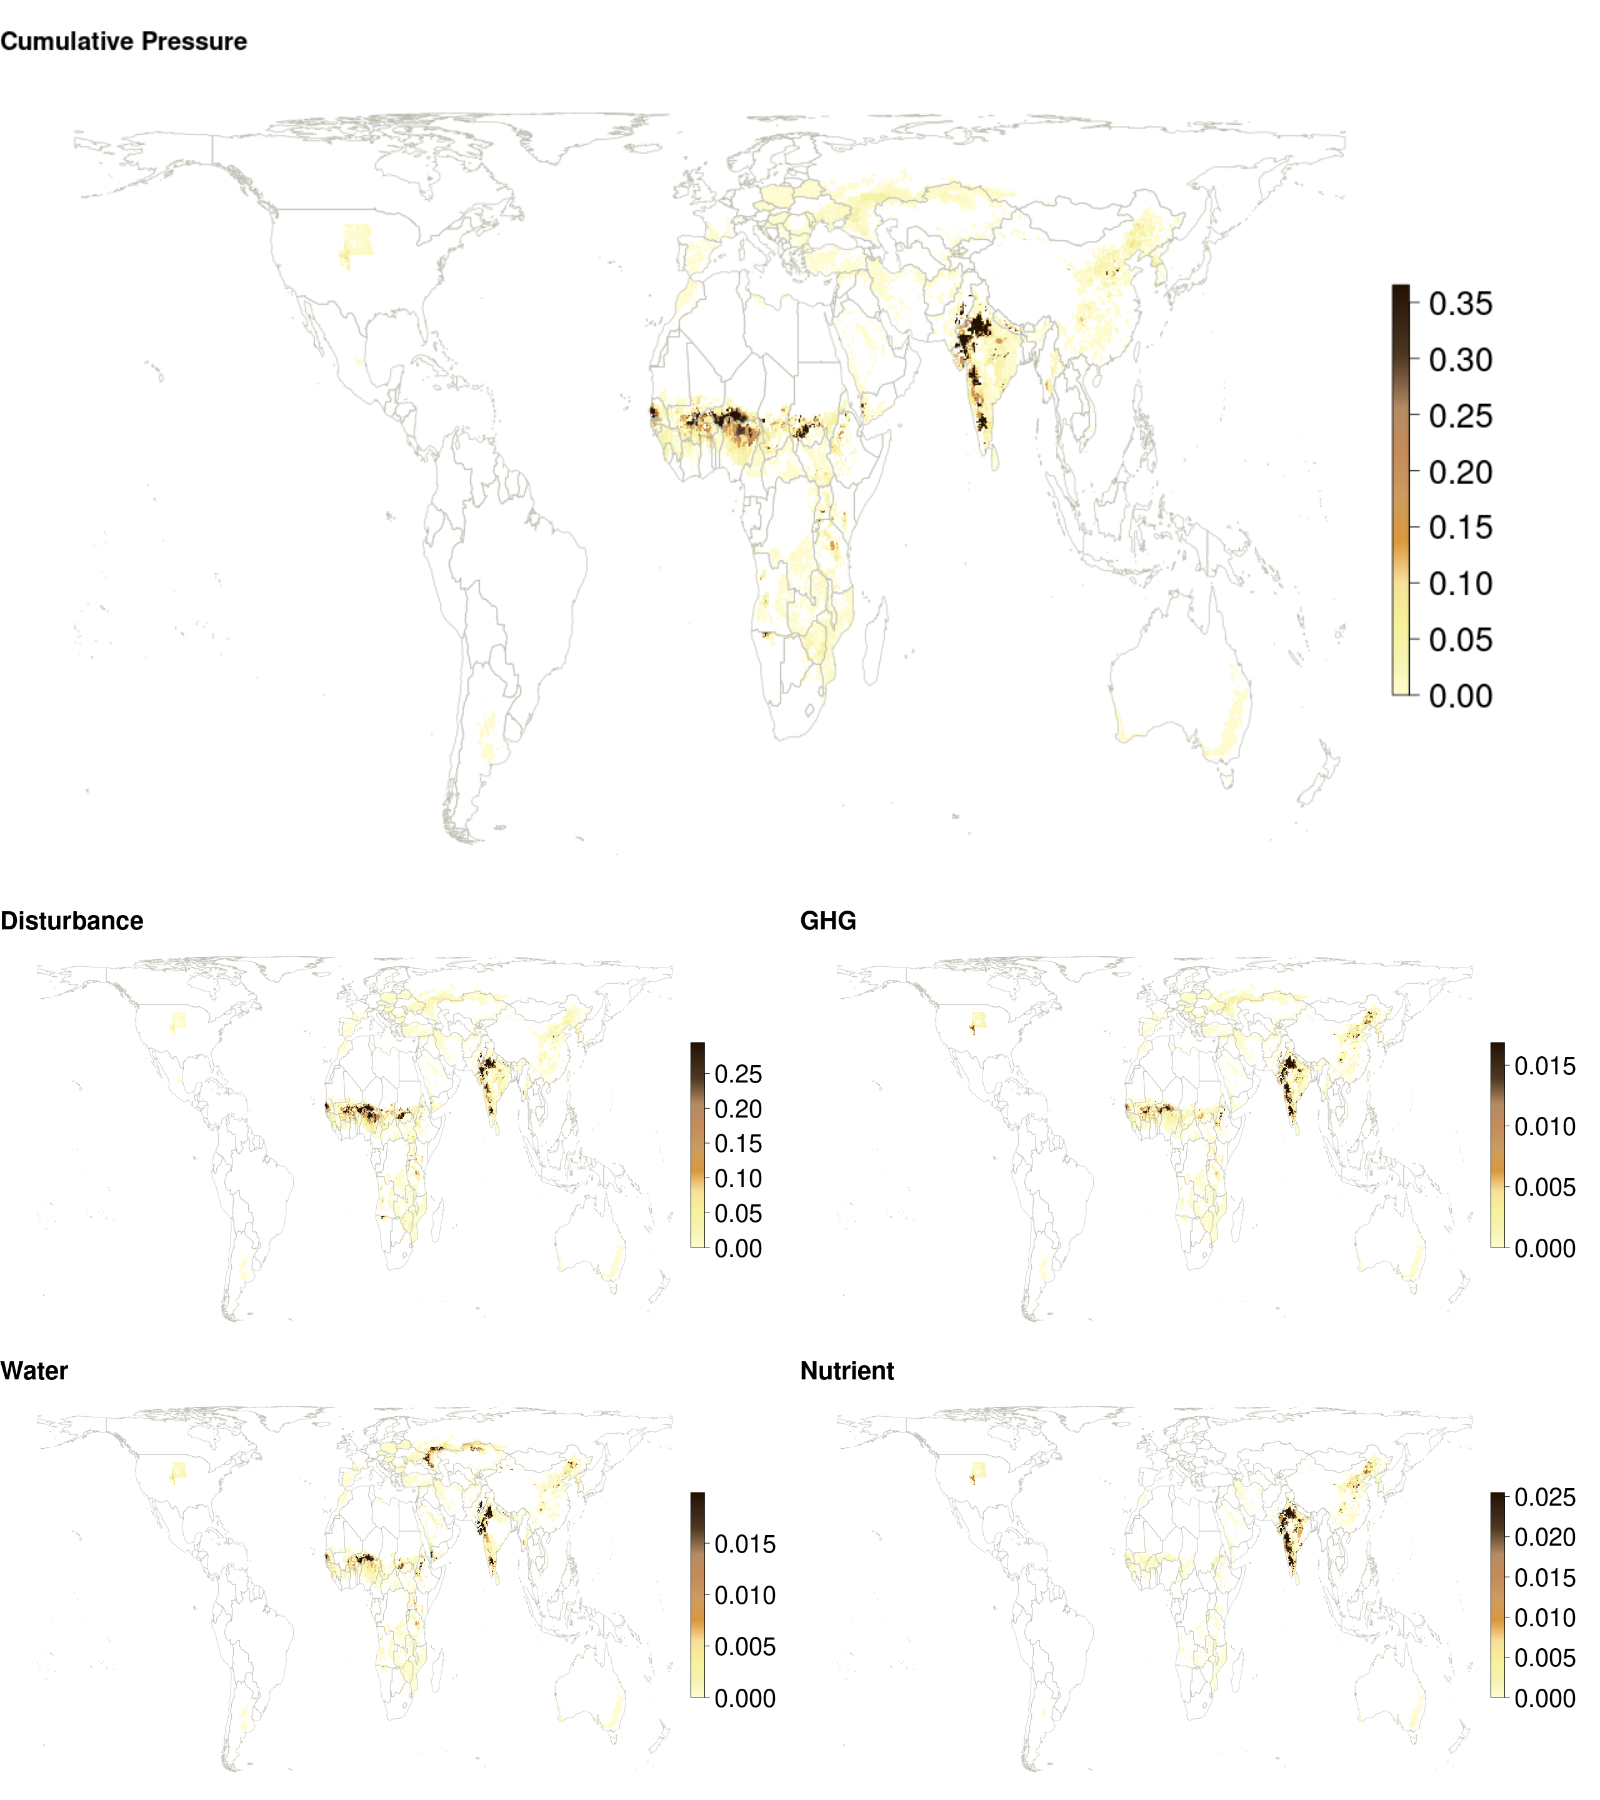
\includegraphics{/home/rayner/food-systems/_analysis/figures/extended_data/output/ed_fig_1_png/xmil_crop_final.png}

\begin{center}\rule{0.5\linewidth}{0.5pt}\end{center}

\hypertarget{other-oil-crops}{%
\subparagraph{25) Other oil crops}\label{other-oil-crops}}

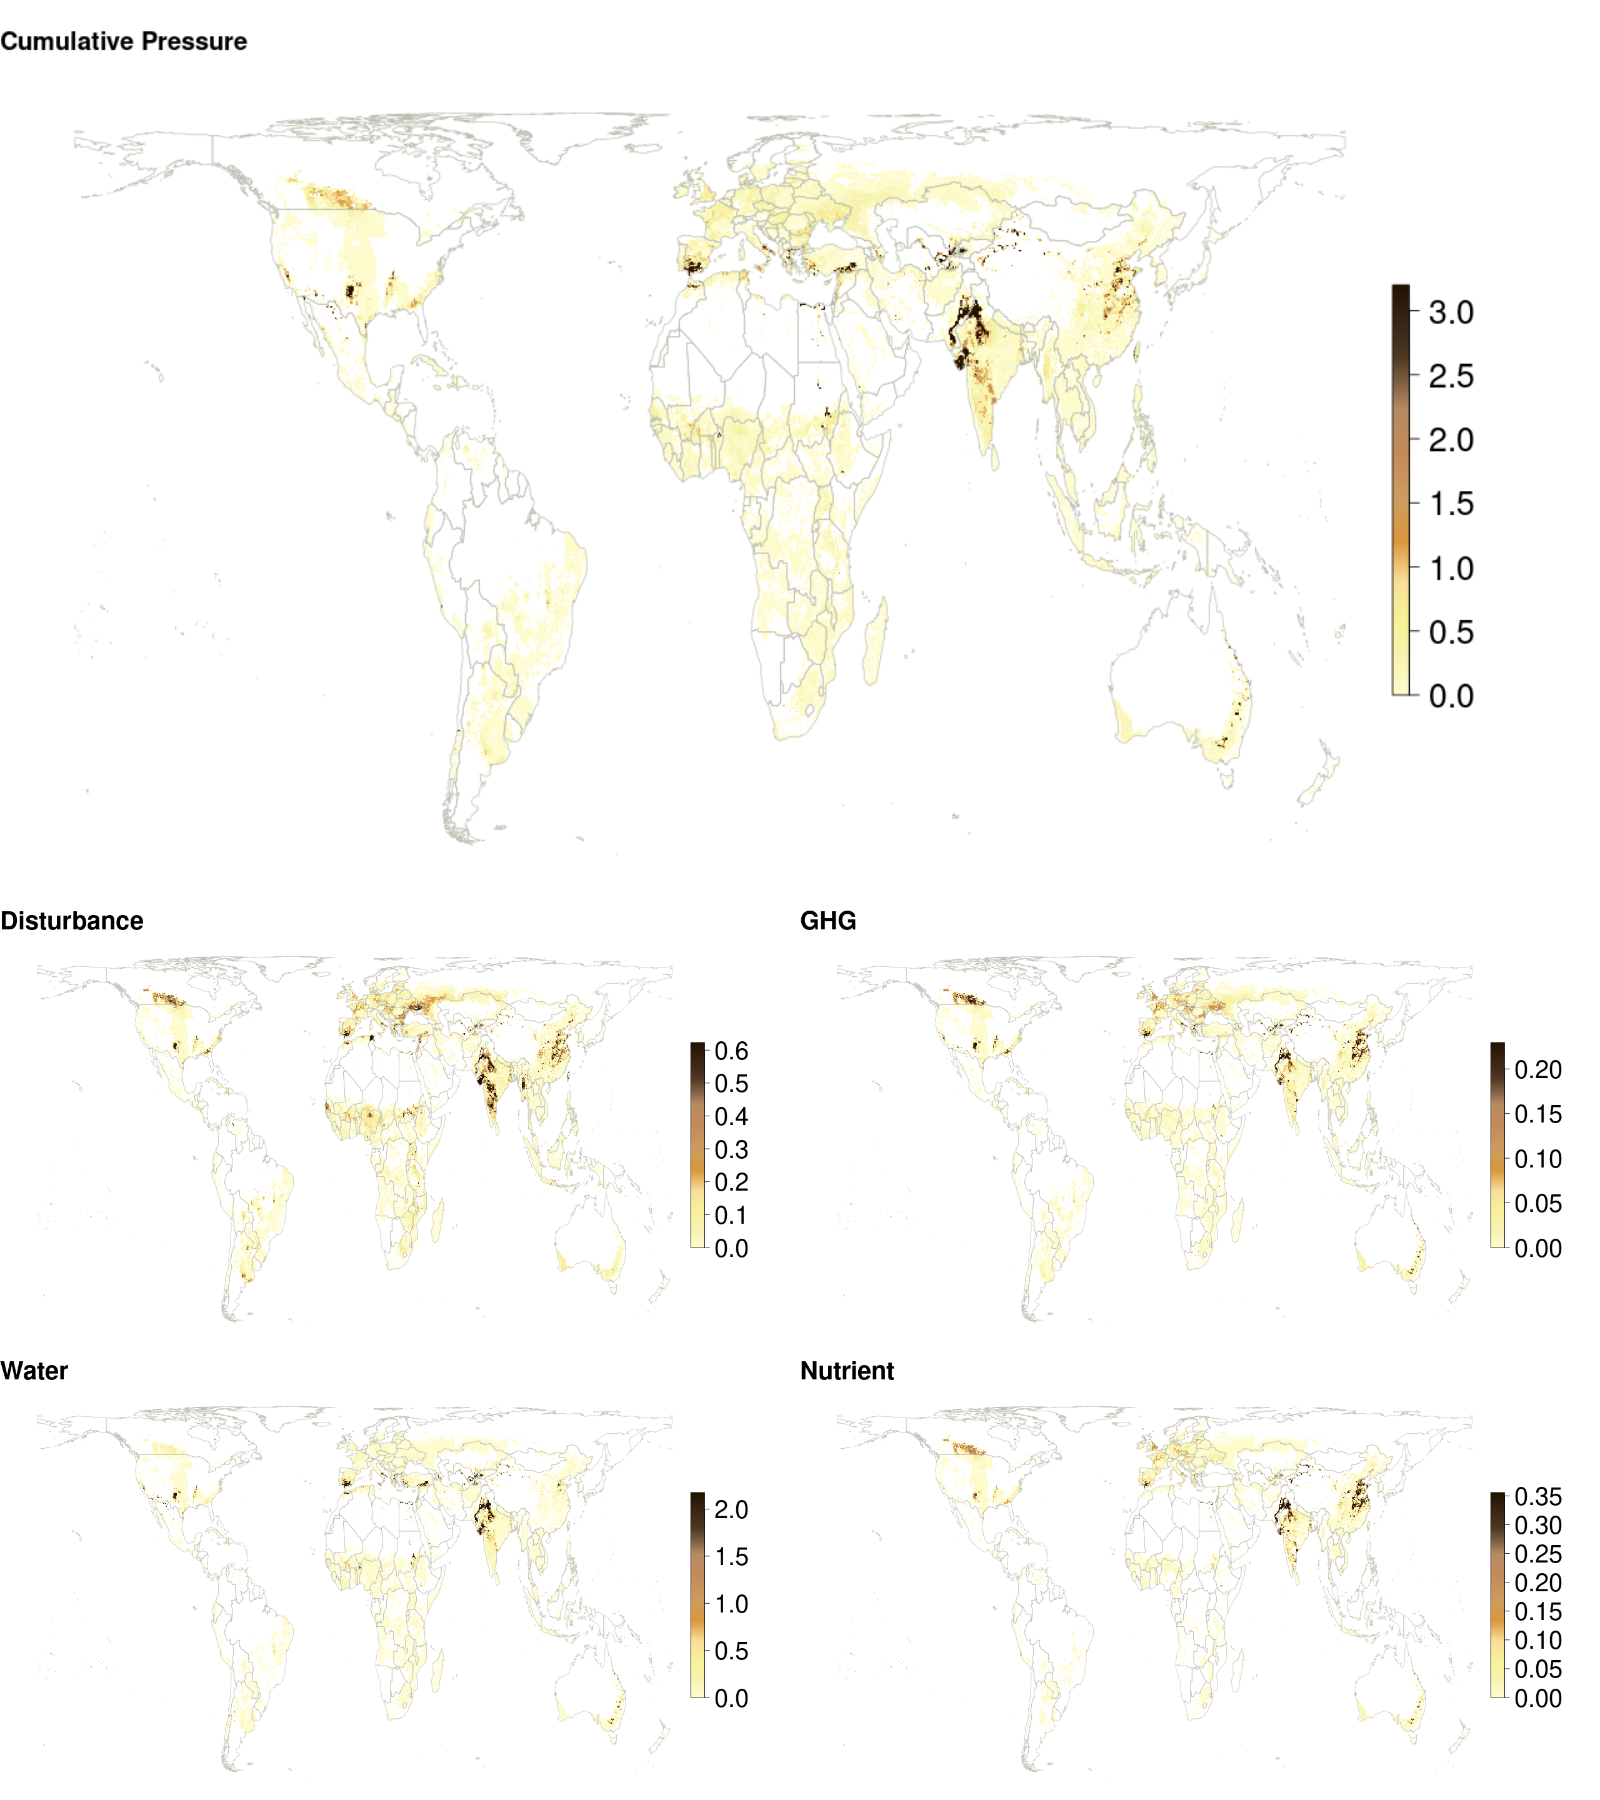
\includegraphics{/home/rayner/food-systems/_analysis/figures/extended_data/output/ed_fig_1_png/xoil_crop_final.png}

\begin{center}\rule{0.5\linewidth}{0.5pt}\end{center}

\hypertarget{other-pulses}{%
\subparagraph{26) Other pulses}\label{other-pulses}}

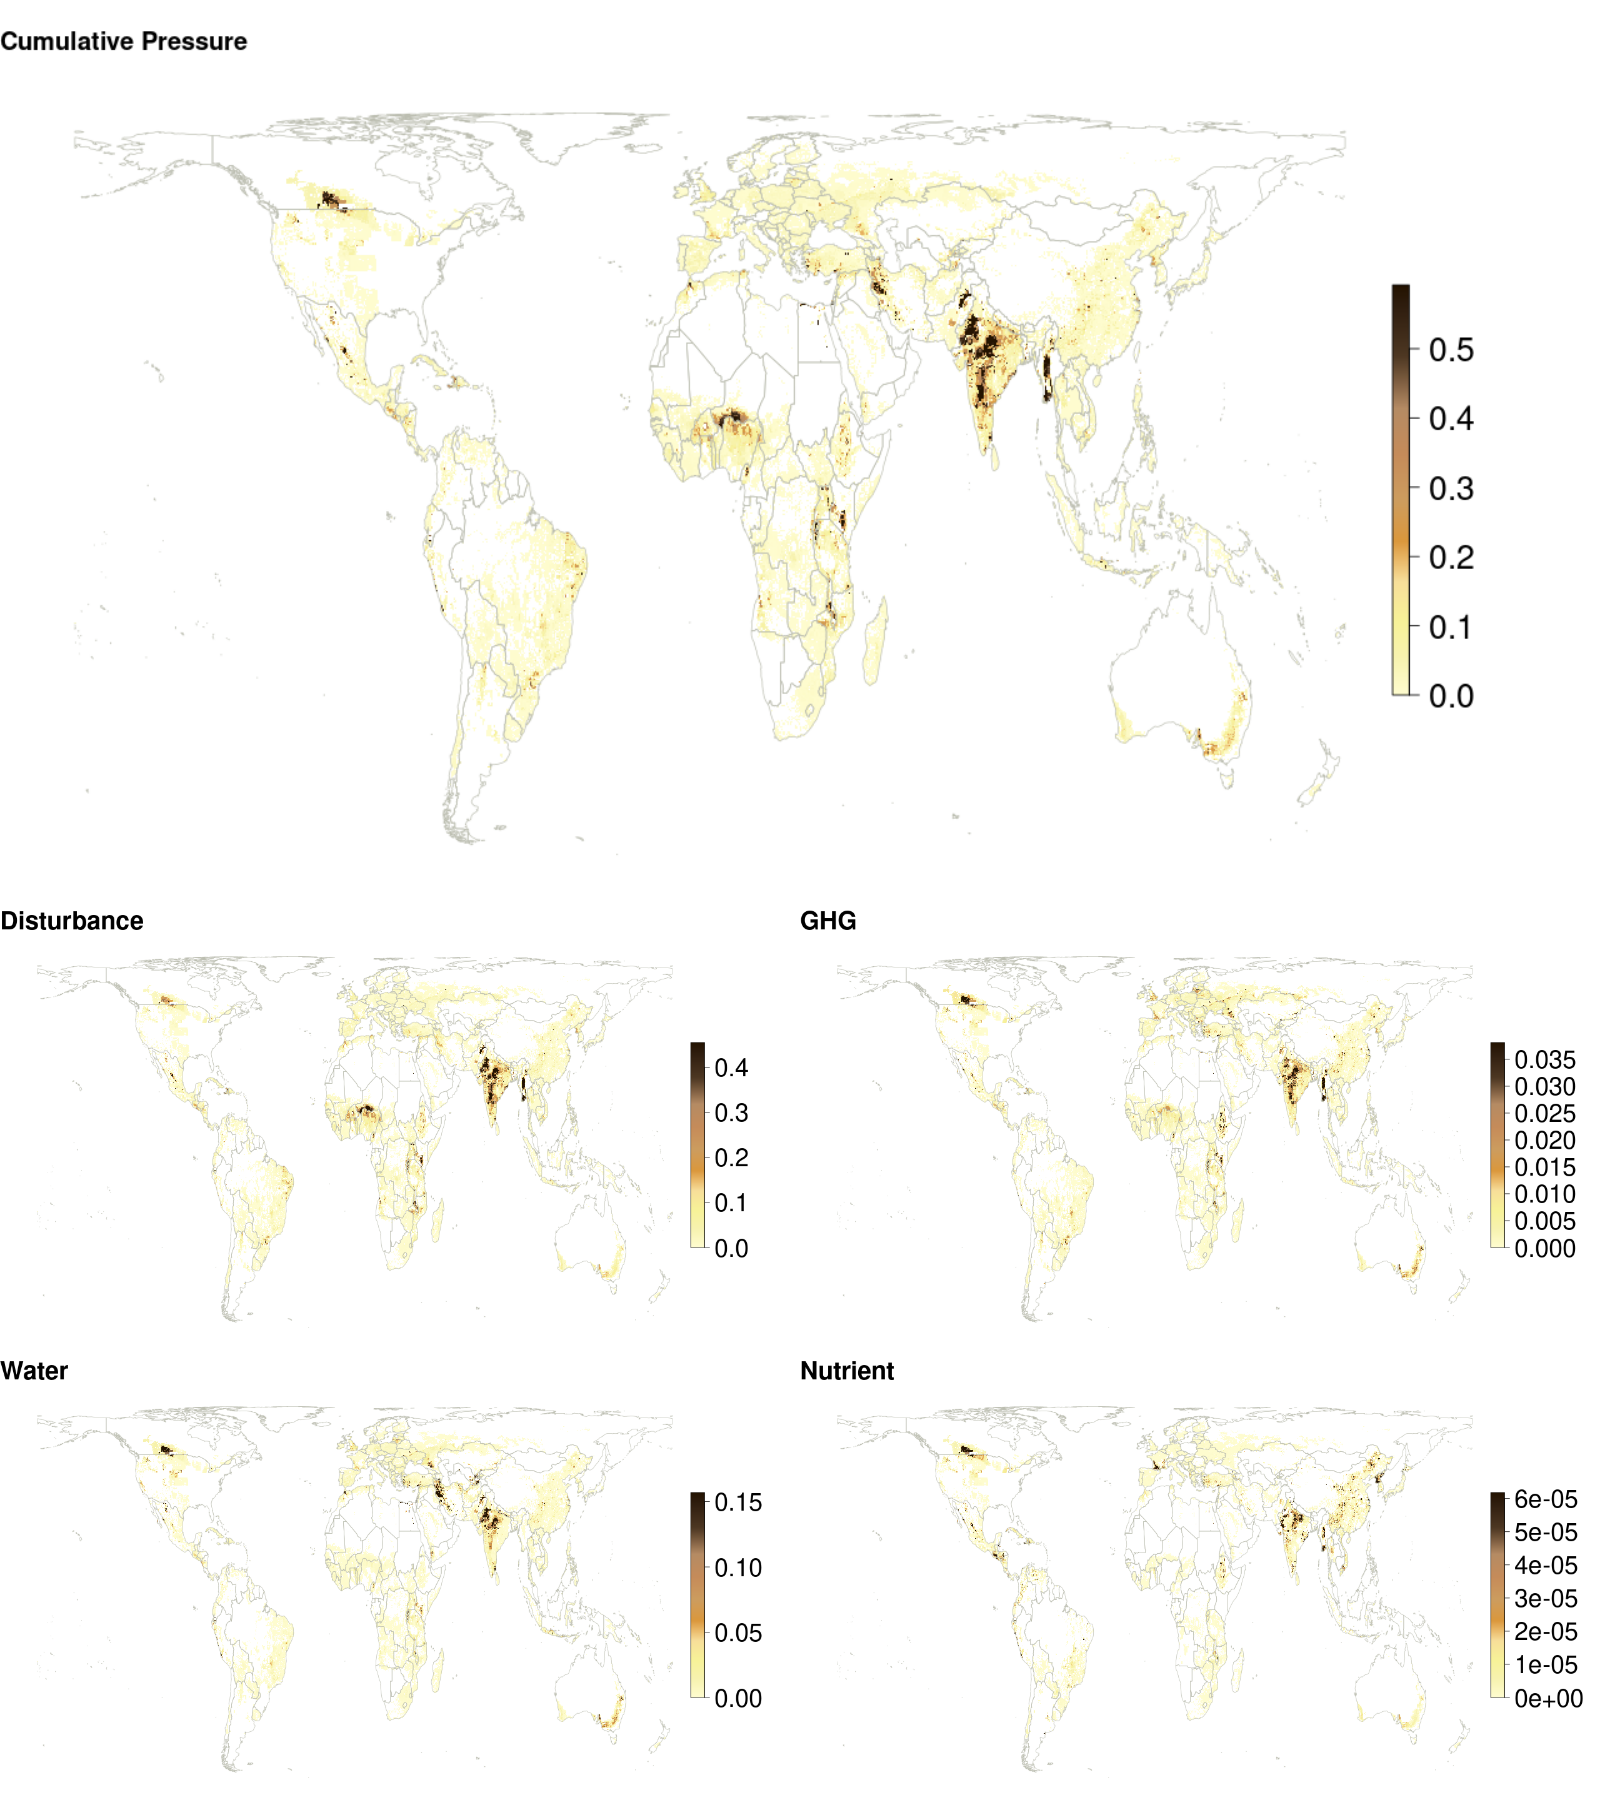
\includegraphics{/home/rayner/food-systems/_analysis/figures/extended_data/output/ed_fig_1_png/xpul_crop_final.png}

\begin{center}\rule{0.5\linewidth}{0.5pt}\end{center}

\hypertarget{yams}{%
\subparagraph{27) Yams}\label{yams}}

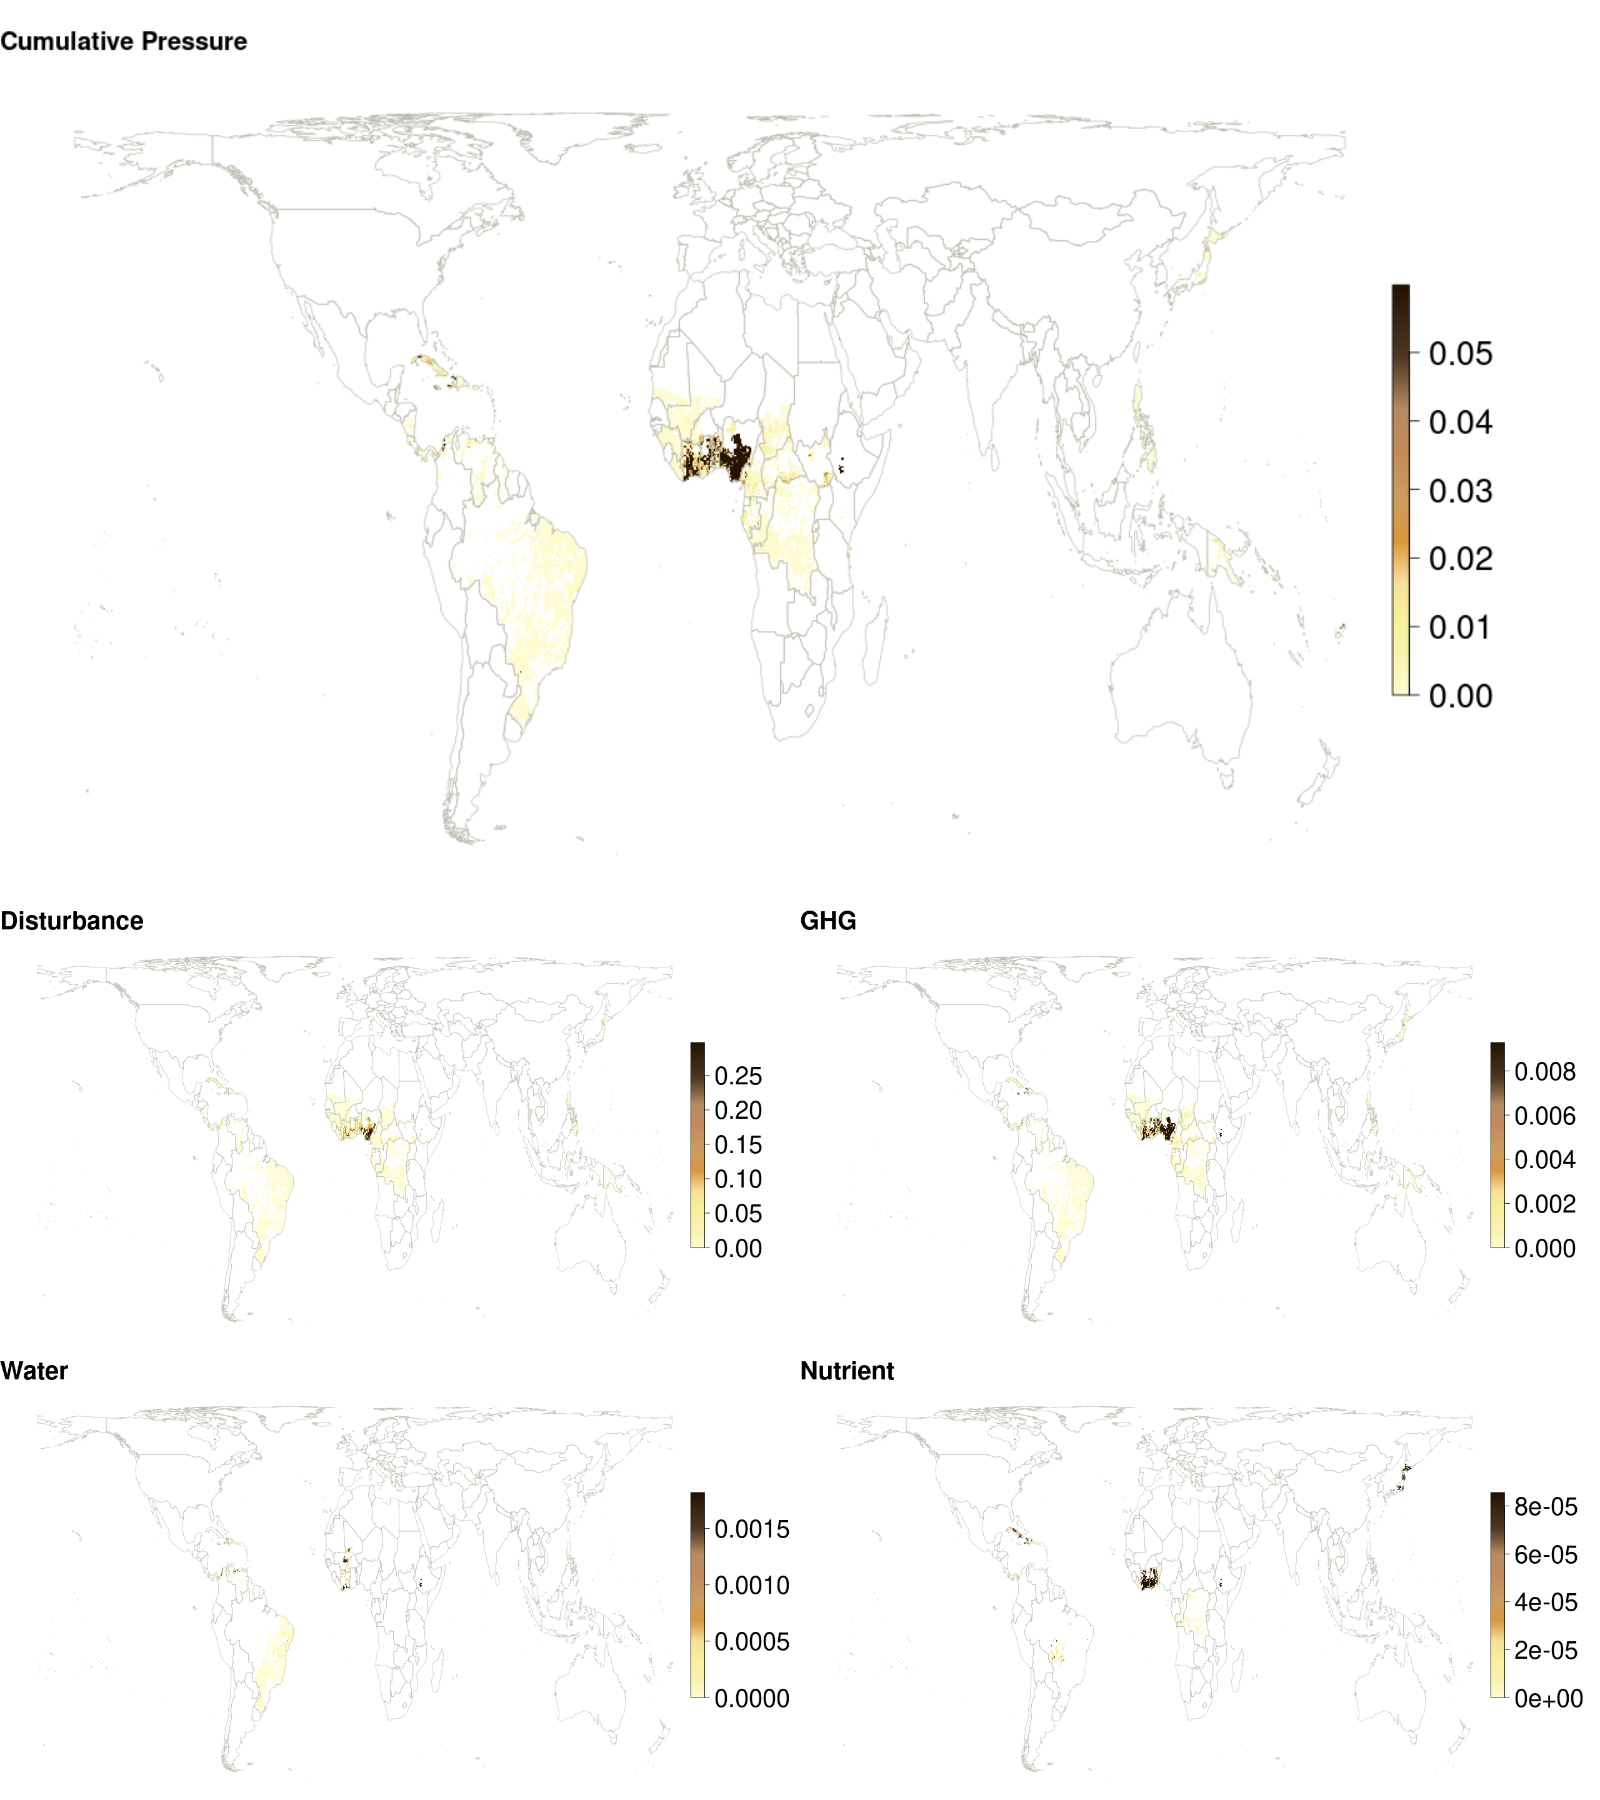
\includegraphics{/home/rayner/food-systems/_analysis/figures/extended_data/output/ed_fig_1_png/yams_crop_final.png}

\begin{center}\rule{0.5\linewidth}{0.5pt}\end{center}

\hypertarget{extended-data-fig.-1b}{%
\paragraph{Extended Data Fig. 1b}\label{extended-data-fig.-1b}}

\textbf{Livestock pressure maps}

Cumulative and individual (disturbance, GHG, water, nutrient) pressures
for eleven livestock categories. Data includes both on-farm pressures
and off-farm feed pressures. The individual pressure maps describe the
rescaled pressure data, calculated by dividing each pixel value (e.g.,
m\textsuperscript{3} water consumption) by the total global pressure
across all food systems and pixels, such that each pixel describes its
proportional contribution to the global total for that pressure. These
values were then multiplied by one million to prevent artefacts from
small values. The cumulative pressure score was calculated by summing
the rescaled pressure layers. Colour ramp scaling is unique to each plot
so the relative spatial distribution of each food item can be more
easily visualised.

\begin{center}\rule{0.5\linewidth}{0.5pt}\end{center}

\hypertarget{buffaloes-milk}{%
\subparagraph{1) Buffaloes milk}\label{buffaloes-milk}}

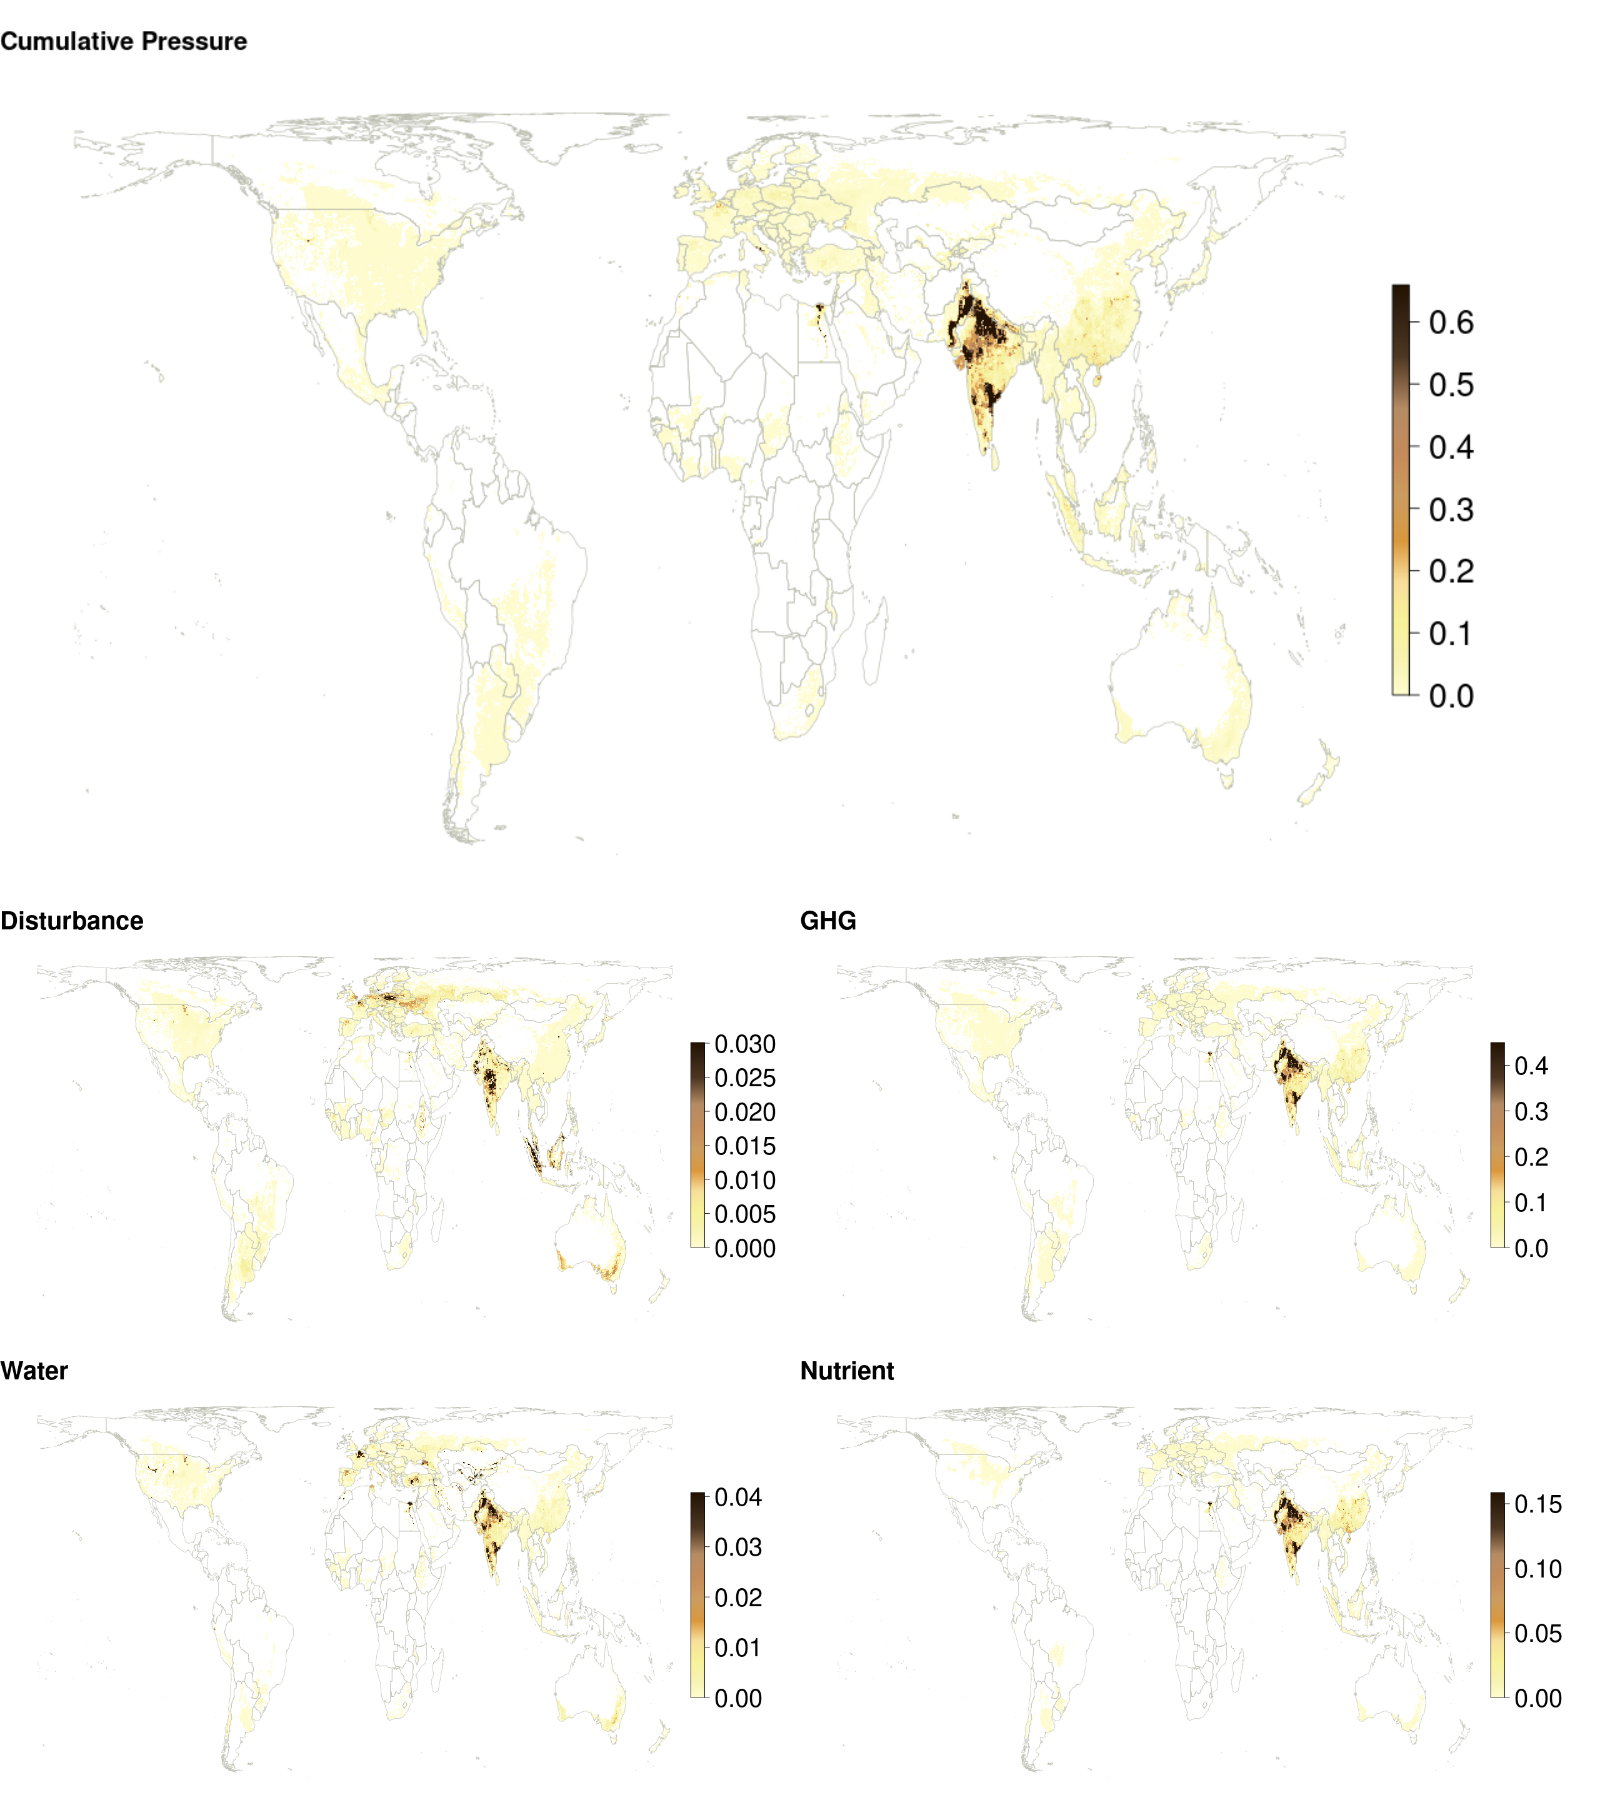
\includegraphics{/home/rayner/food-systems/_analysis/figures/extended_data/output/ed_fig_1_png/buffaloes_milk_final.png}

\begin{center}\rule{0.5\linewidth}{0.5pt}\end{center}

\hypertarget{chickens-eggs}{%
\subparagraph{2) Chickens eggs}\label{chickens-eggs}}

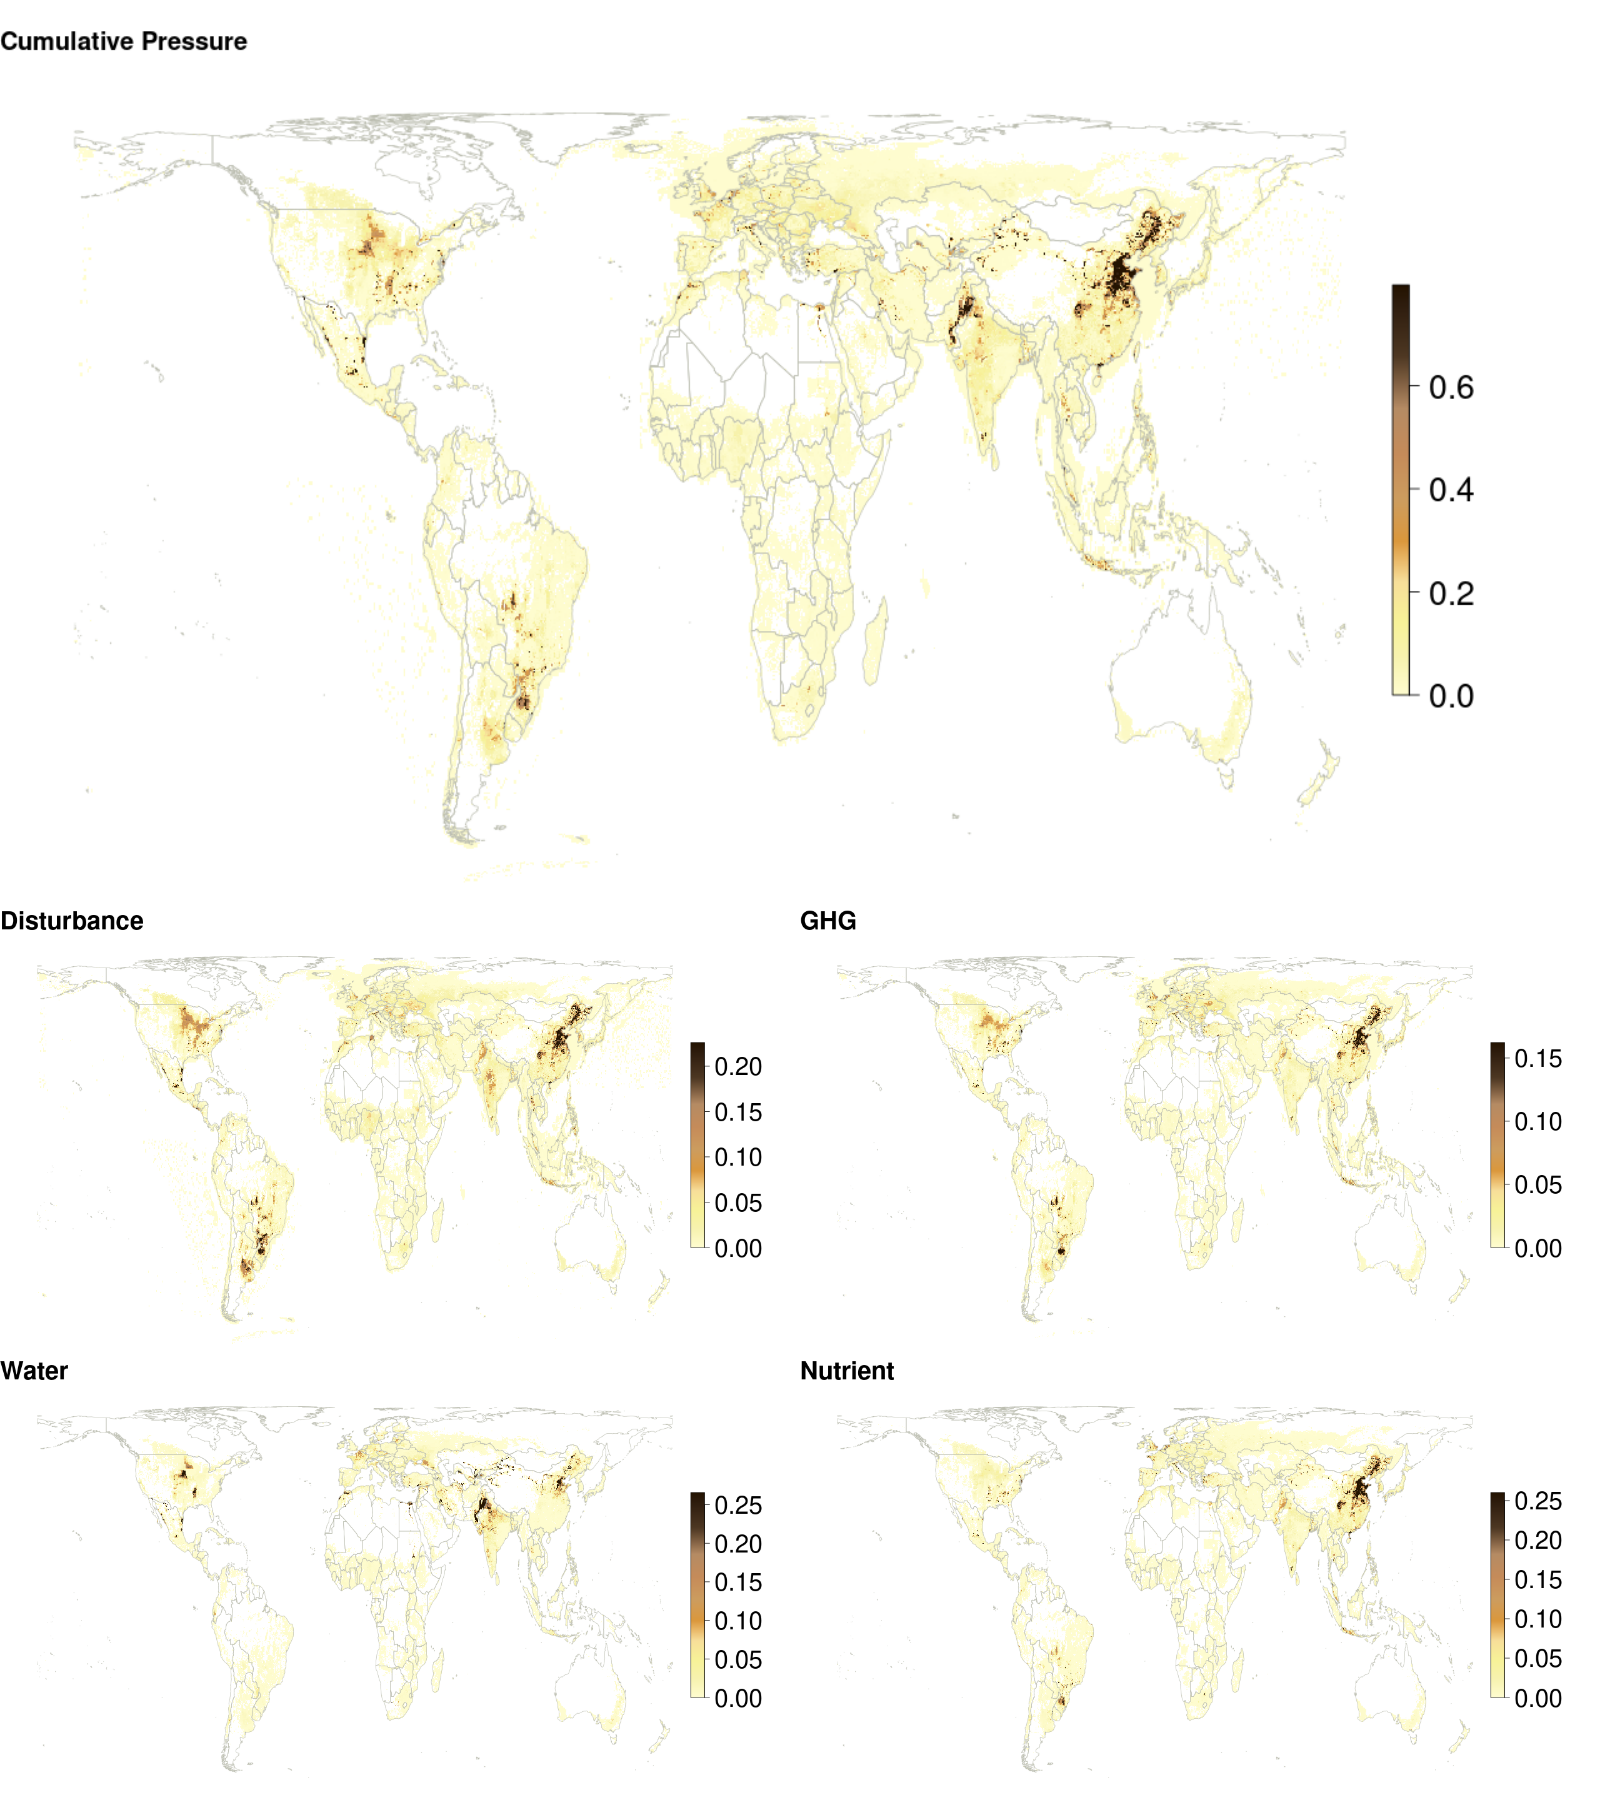
\includegraphics{/home/rayner/food-systems/_analysis/figures/extended_data/output/ed_fig_1_png/chickens_eggs_final.png}

\begin{center}\rule{0.5\linewidth}{0.5pt}\end{center}

\hypertarget{chickens-eggs-and-meat}{%
\subparagraph{3) Chickens eggs and meat}\label{chickens-eggs-and-meat}}

\includegraphics{/home/rayner/food-systems/_analysis/figures/extended_data/output/ed_fig_1_png/chickens_eggs\&meat_final.png}

\begin{center}\rule{0.5\linewidth}{0.5pt}\end{center}

\hypertarget{chickens-meat}{%
\subparagraph{4) Chickens meat}\label{chickens-meat}}

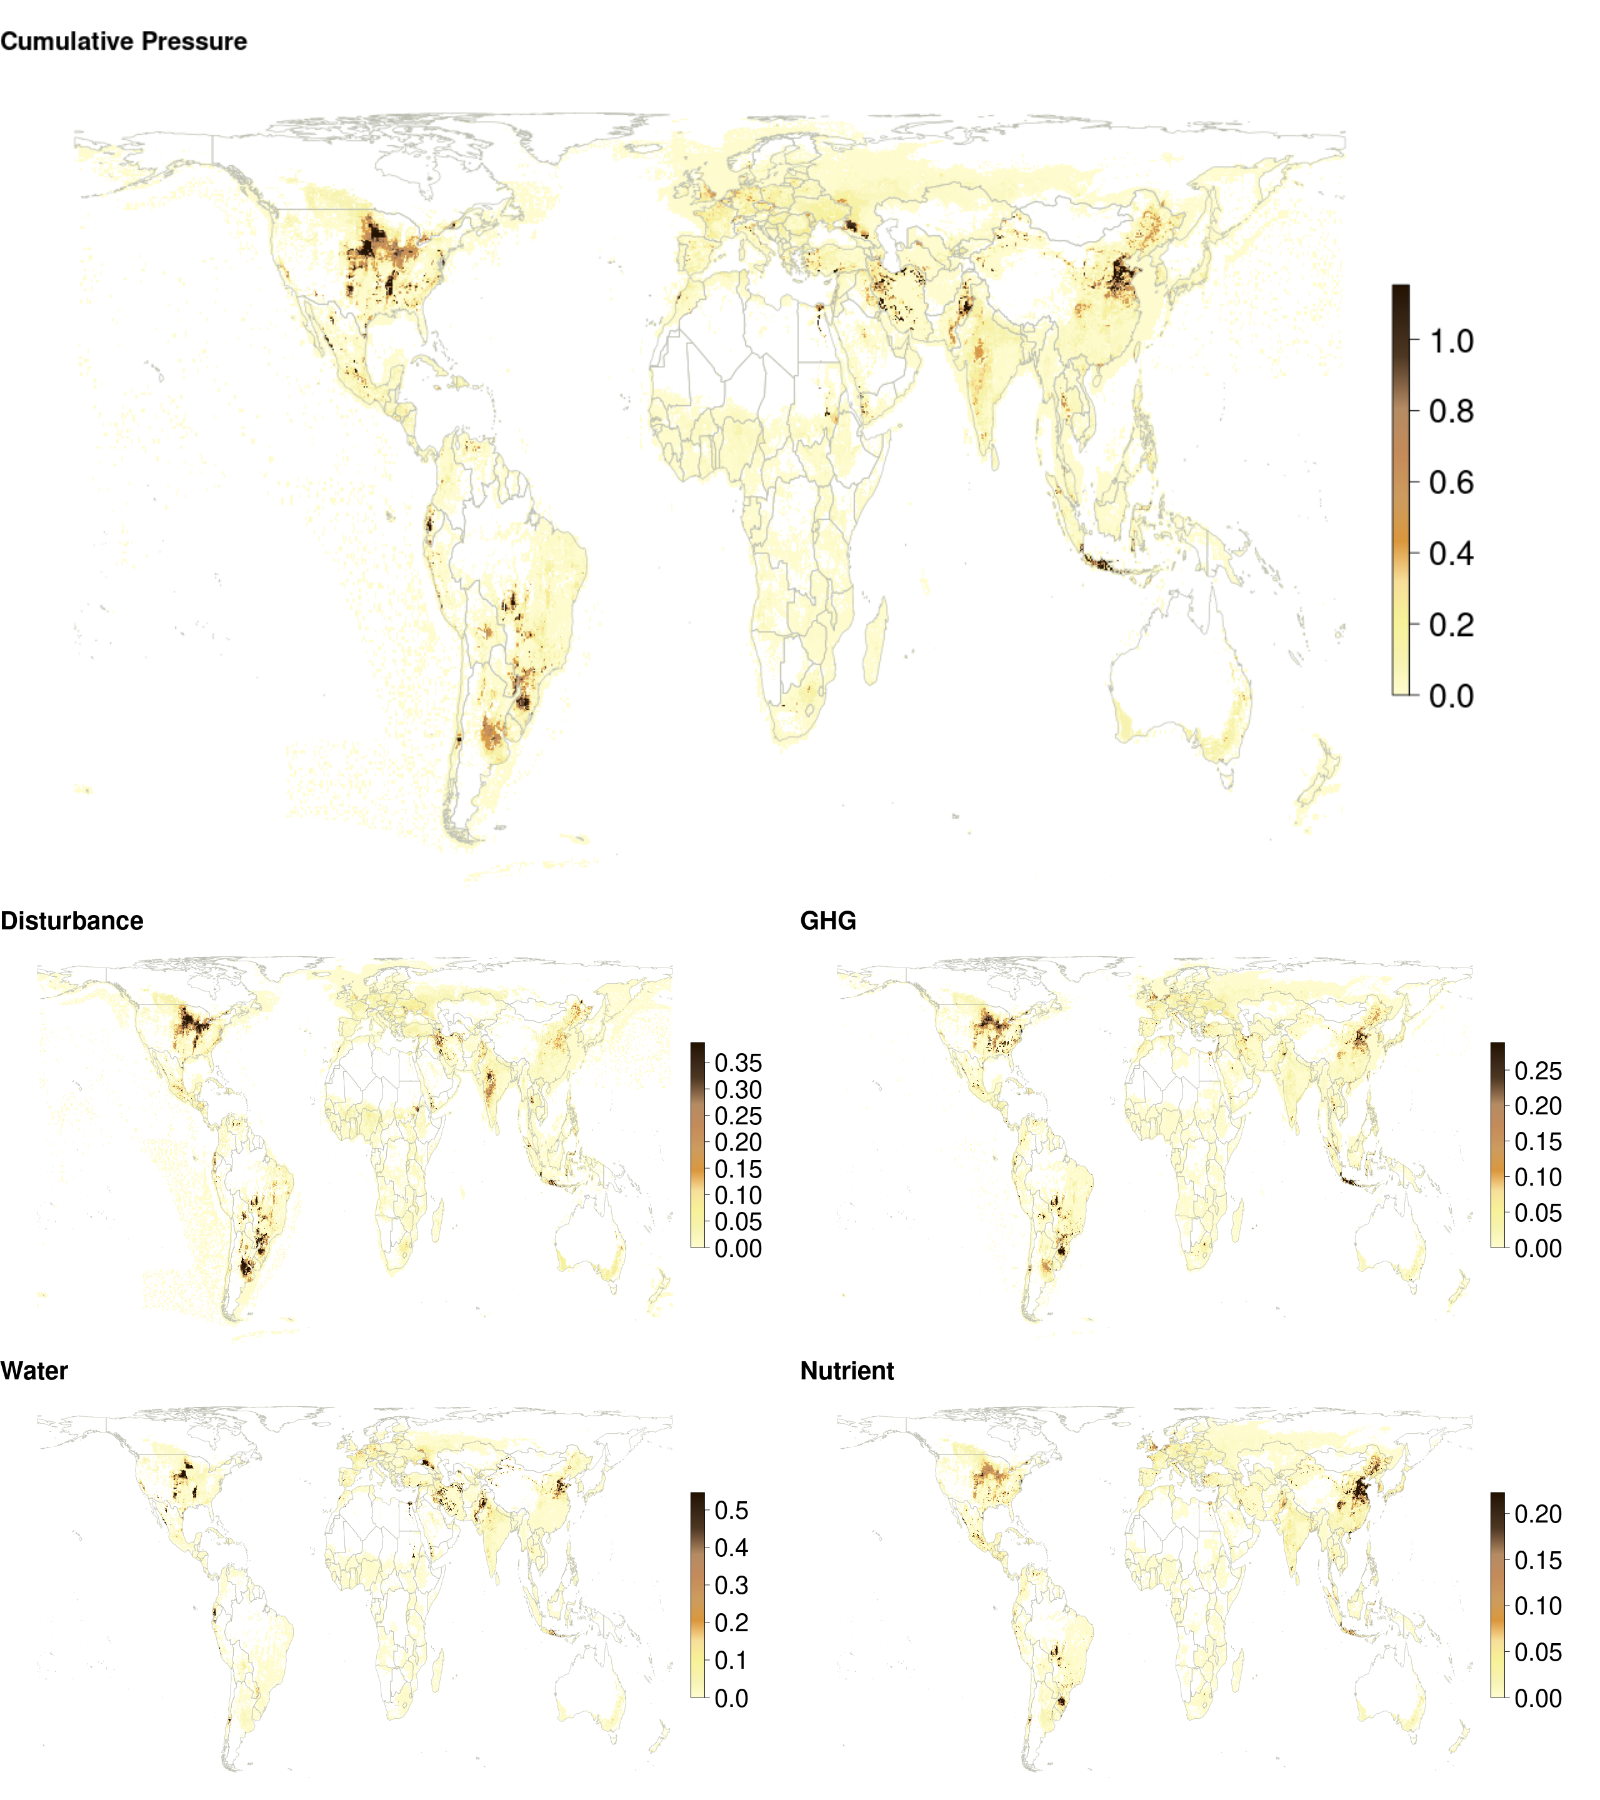
\includegraphics{/home/rayner/food-systems/_analysis/figures/extended_data/output/ed_fig_1_png/chickens_meat_final.png}

\begin{center}\rule{0.5\linewidth}{0.5pt}\end{center}

\hypertarget{cows-meat}{%
\subparagraph{5) Cows meat}\label{cows-meat}}

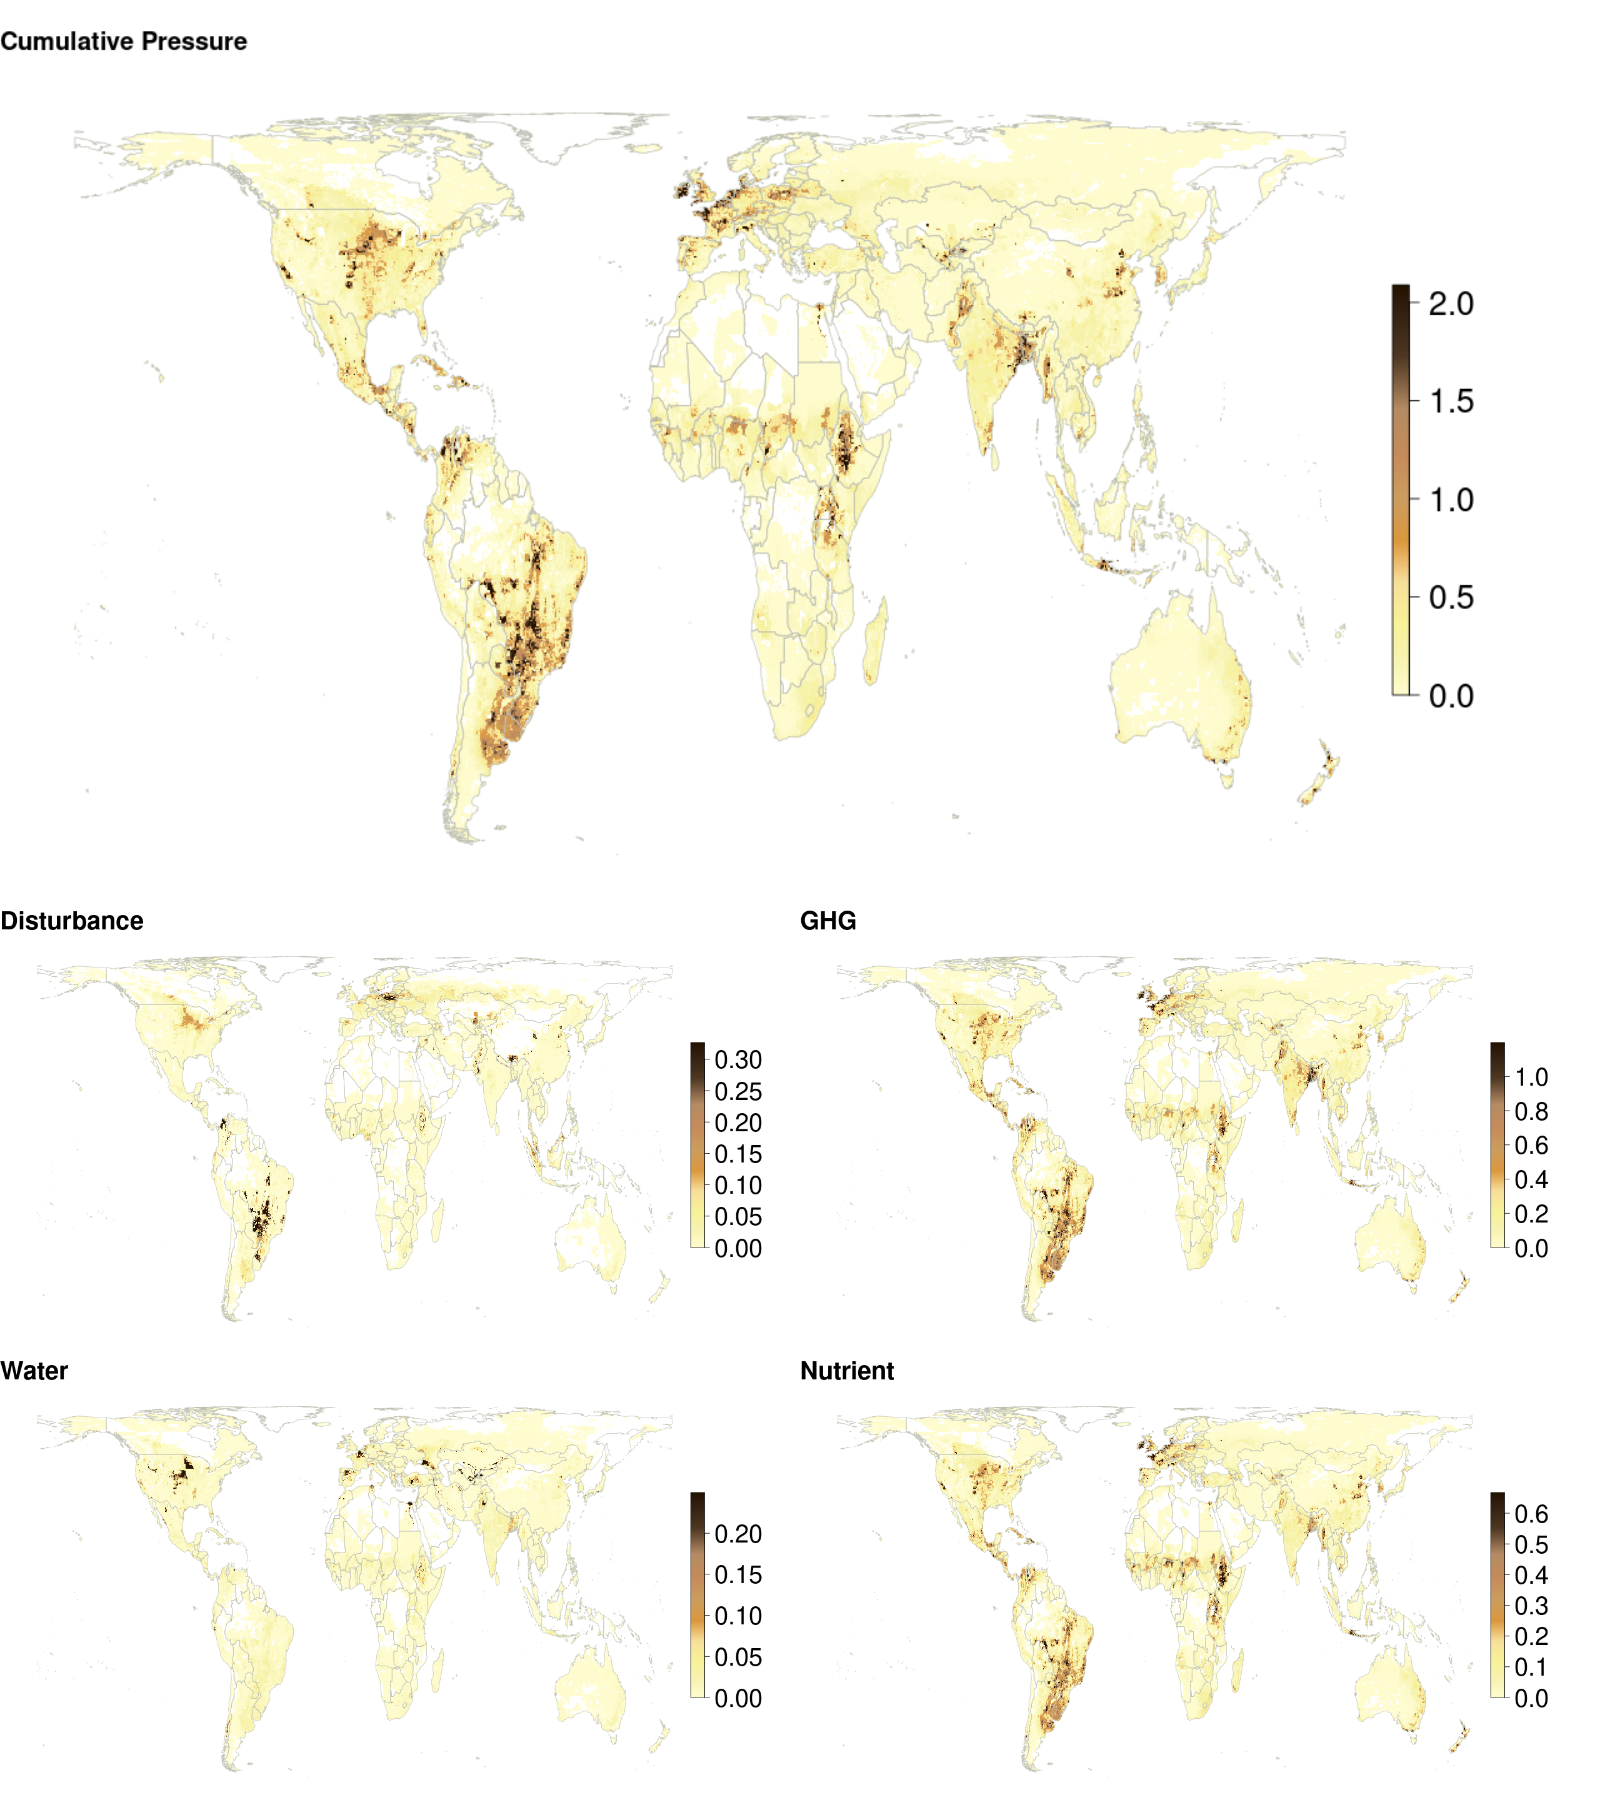
\includegraphics{/home/rayner/food-systems/_analysis/figures/extended_data/output/ed_fig_1_png/cows_meat_final.png}

\begin{center}\rule{0.5\linewidth}{0.5pt}\end{center}

\hypertarget{cows-milk}{%
\subparagraph{6) Cows milk}\label{cows-milk}}

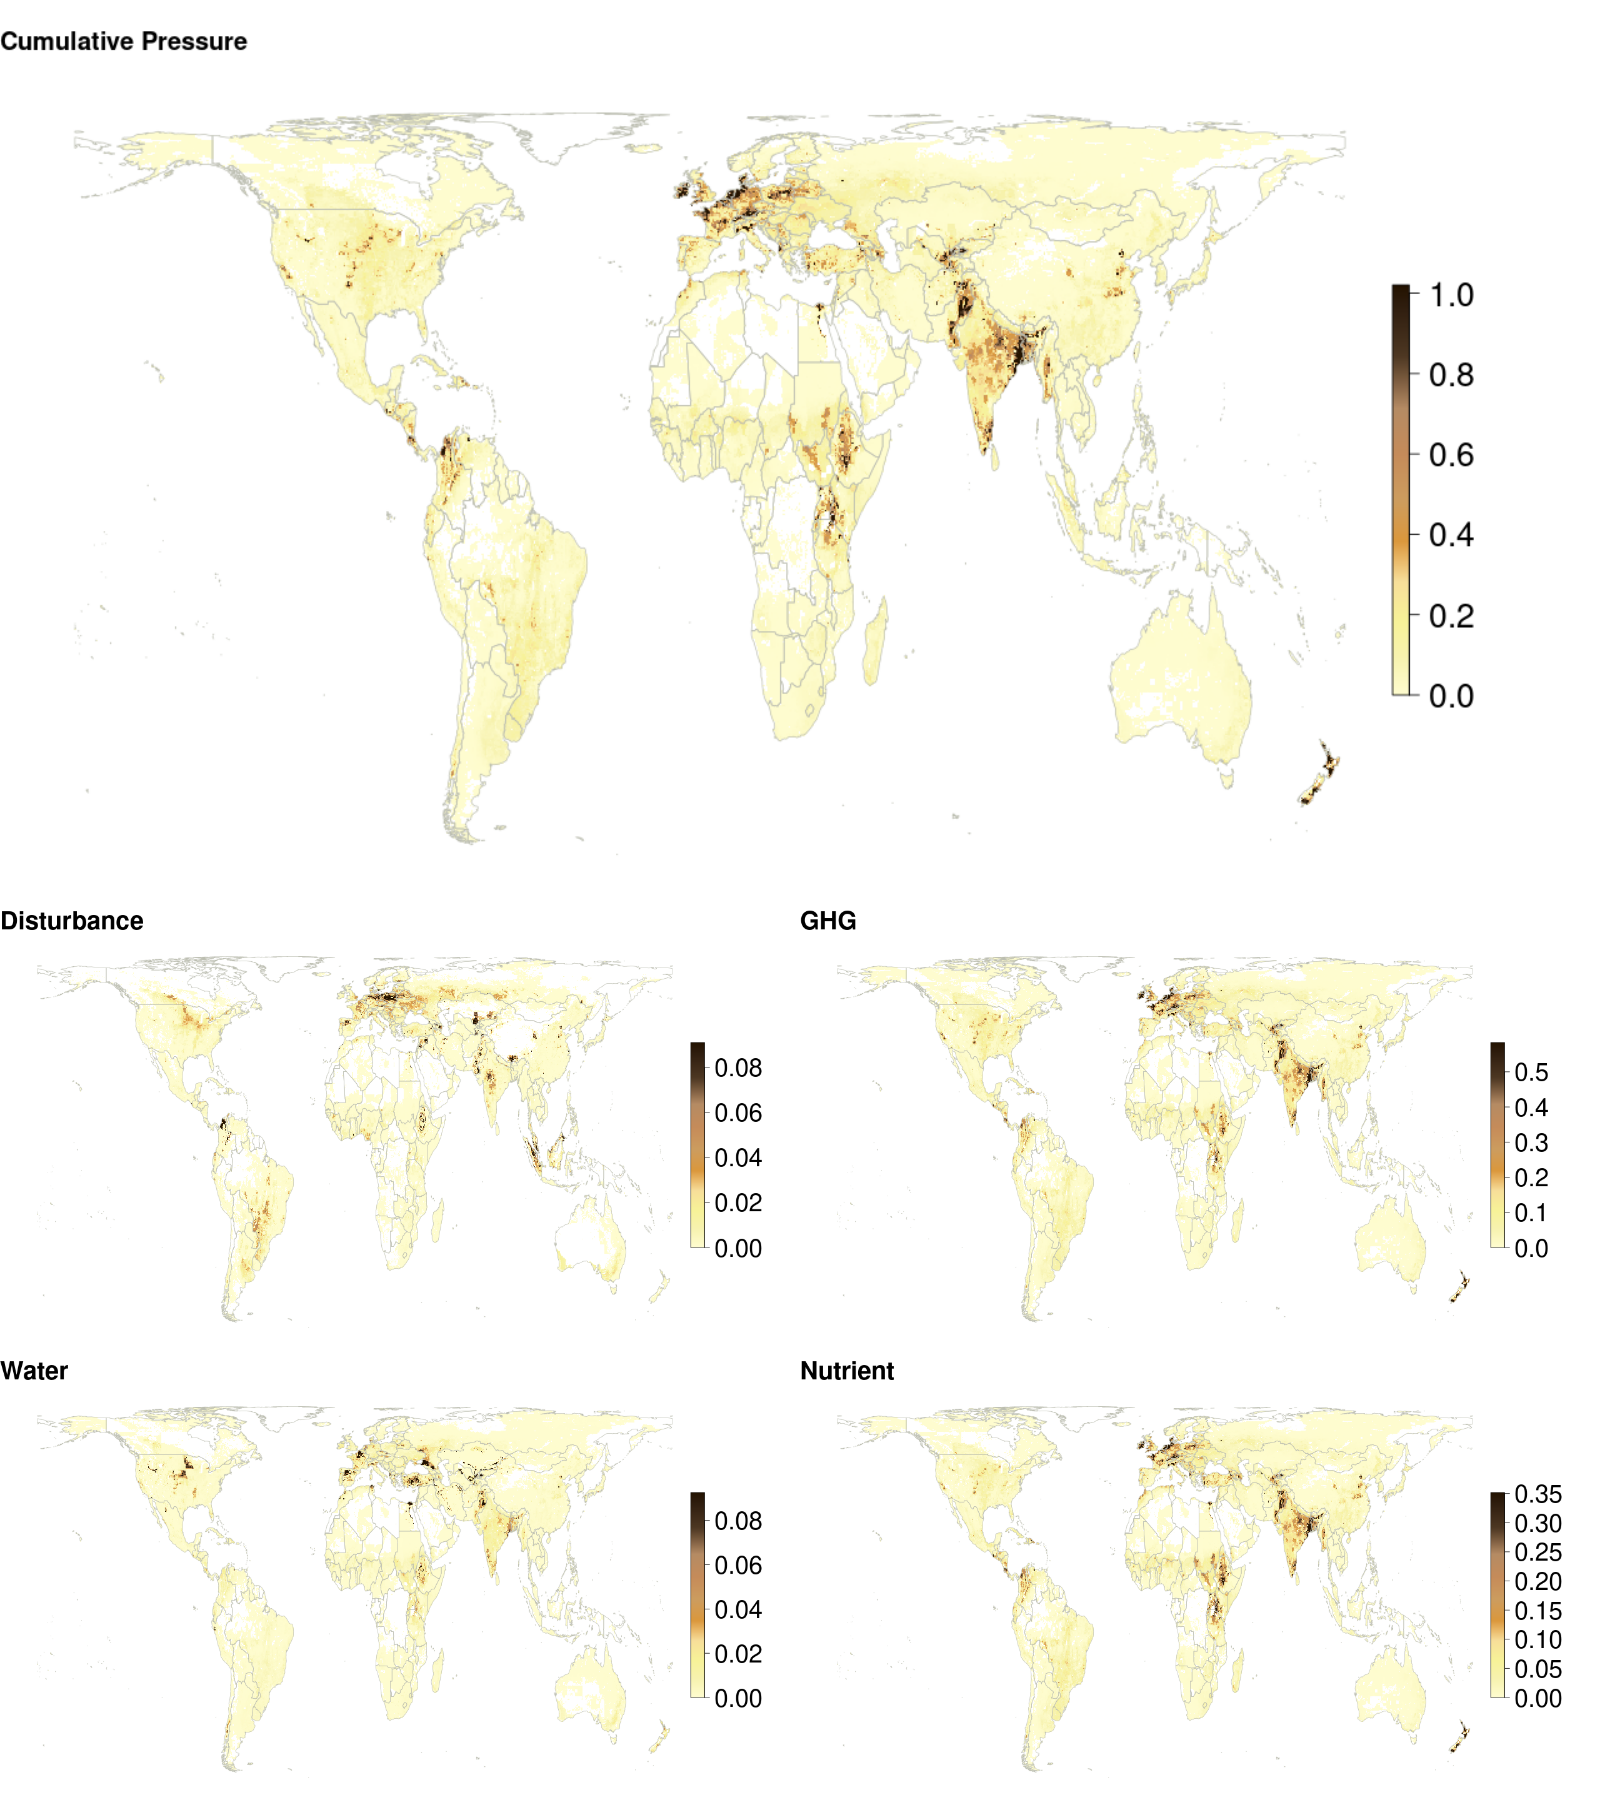
\includegraphics{/home/rayner/food-systems/_analysis/figures/extended_data/output/ed_fig_1_png/cows_milk_final.png}

\begin{center}\rule{0.5\linewidth}{0.5pt}\end{center}

\hypertarget{goats-meat}{%
\subparagraph{7) Goats meat}\label{goats-meat}}

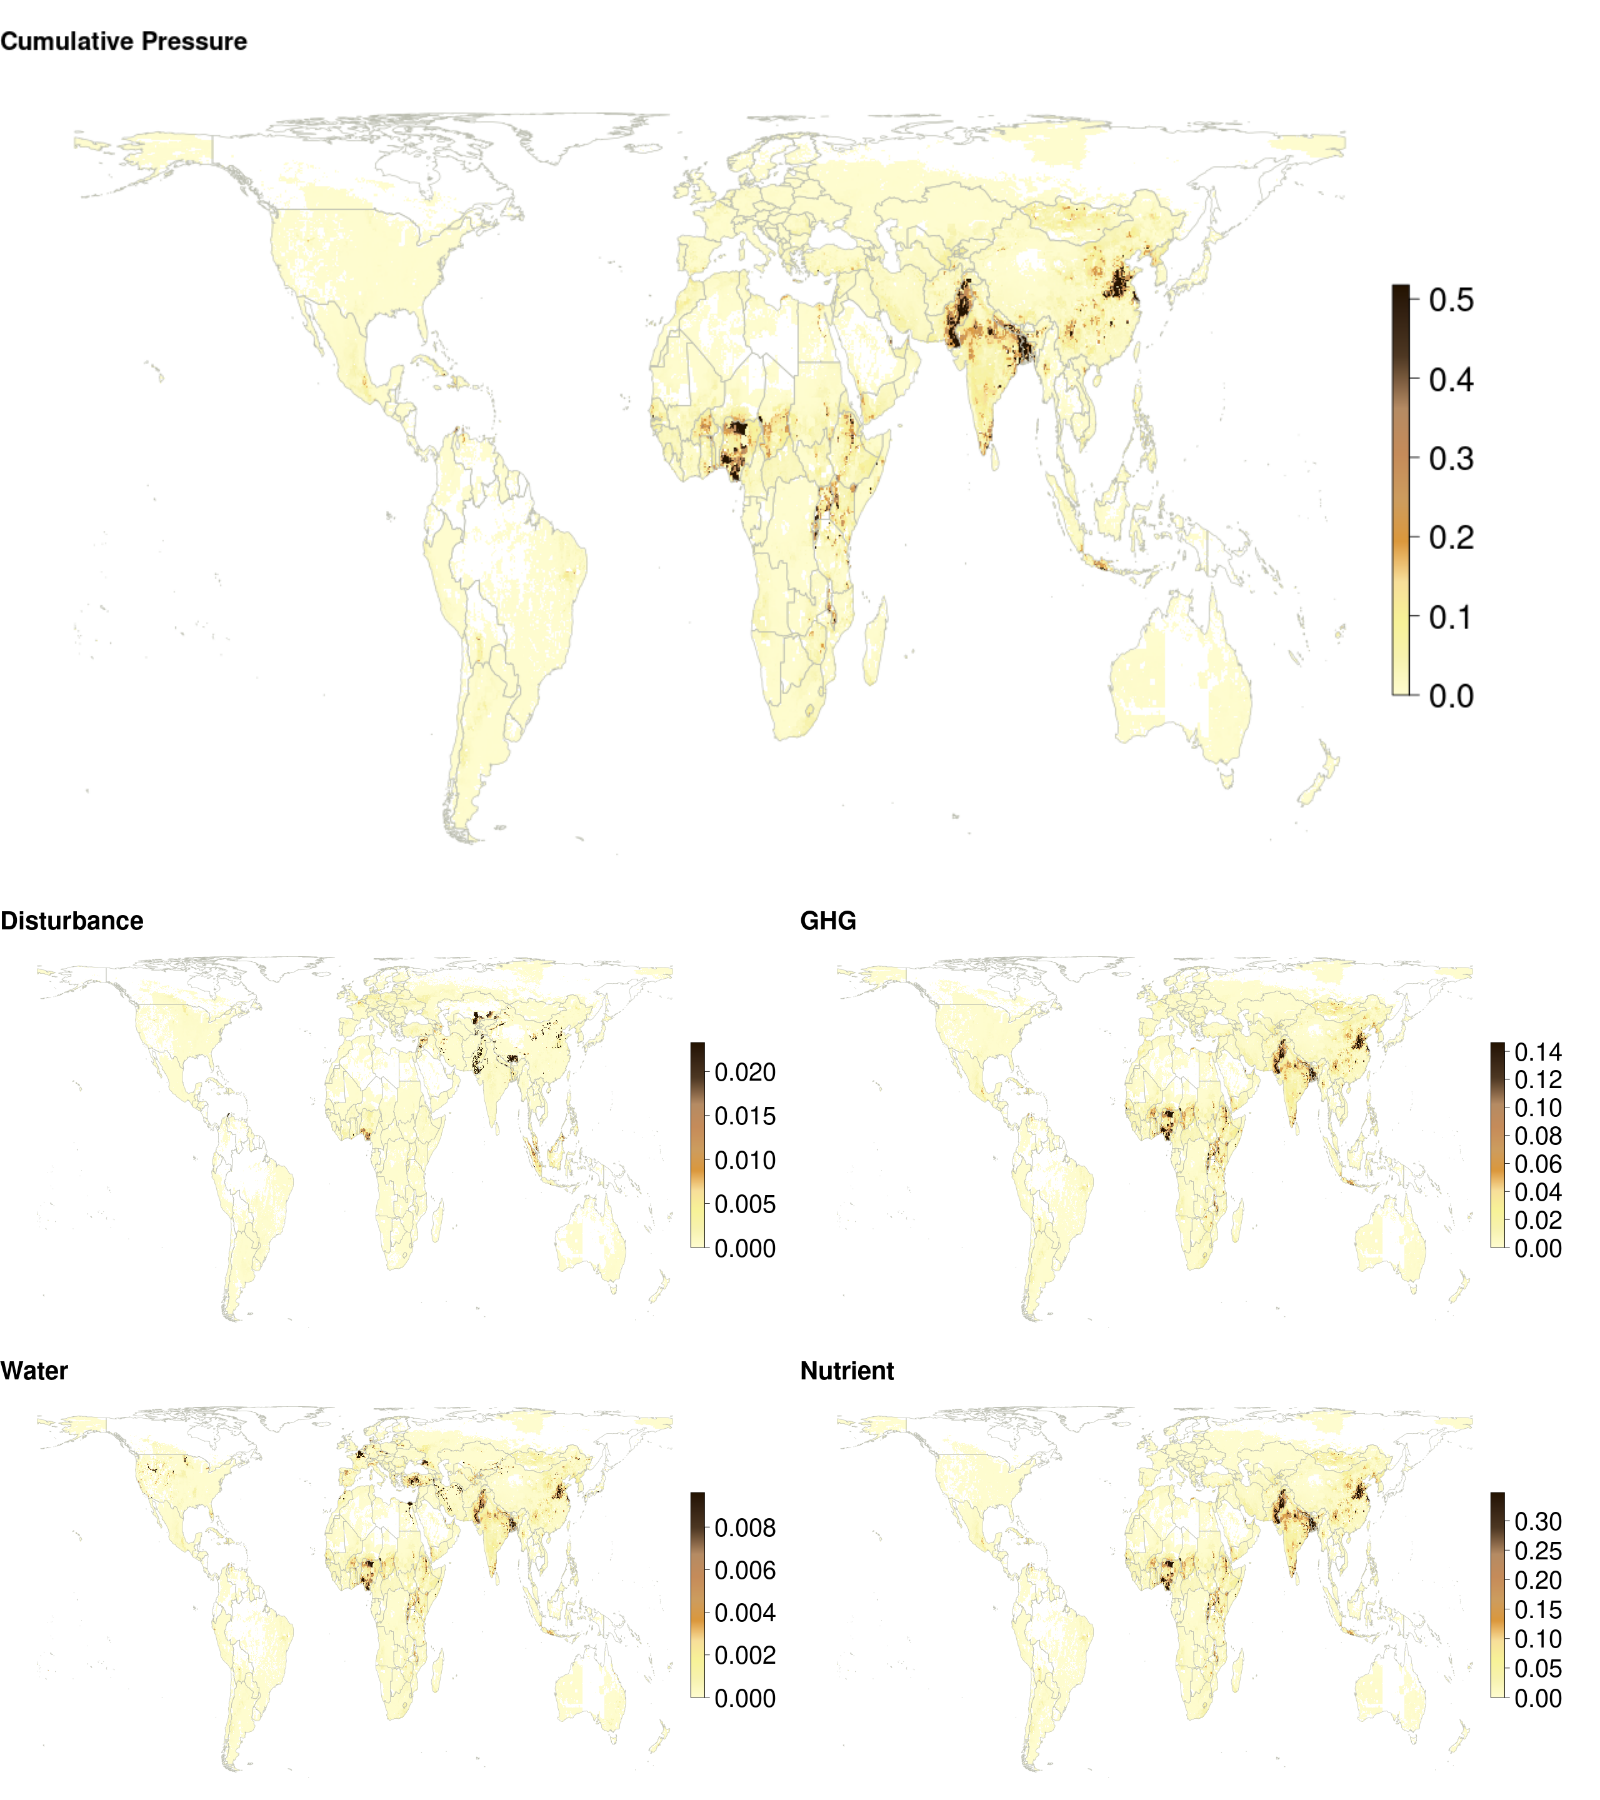
\includegraphics{/home/rayner/food-systems/_analysis/figures/extended_data/output/ed_fig_1_png/goats_meat_final.png}

\begin{center}\rule{0.5\linewidth}{0.5pt}\end{center}

\hypertarget{goats-milk}{%
\subparagraph{8) Goats milk}\label{goats-milk}}

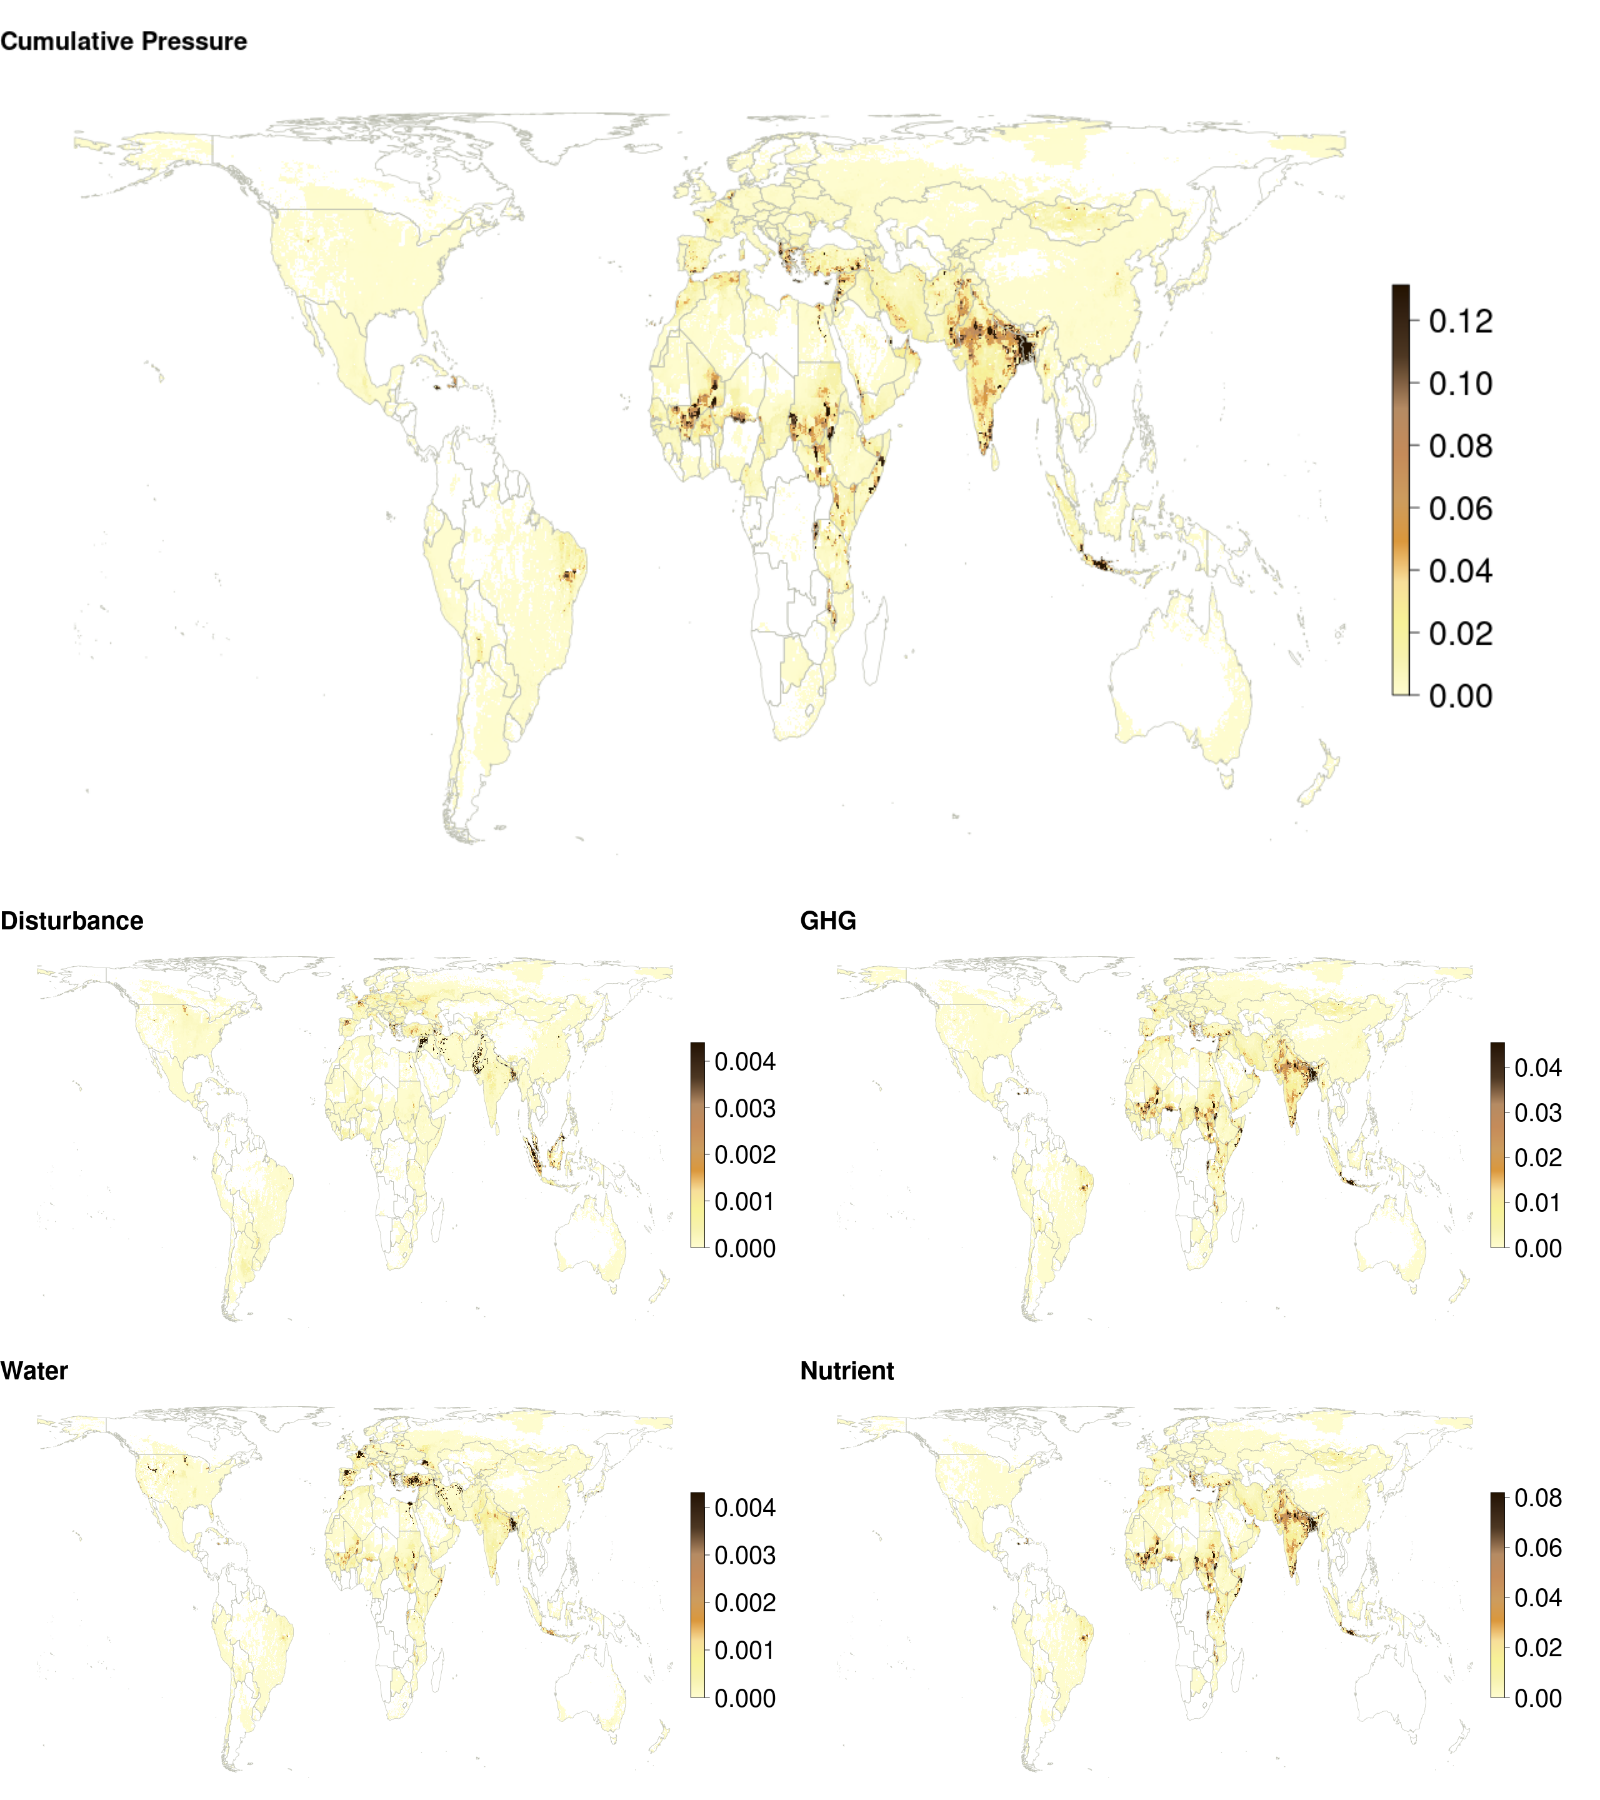
\includegraphics{/home/rayner/food-systems/_analysis/figures/extended_data/output/ed_fig_1_png/goats_milk_final.png}

\begin{center}\rule{0.5\linewidth}{0.5pt}\end{center}

\hypertarget{pigs-meat}{%
\subparagraph{9) Pigs meat}\label{pigs-meat}}

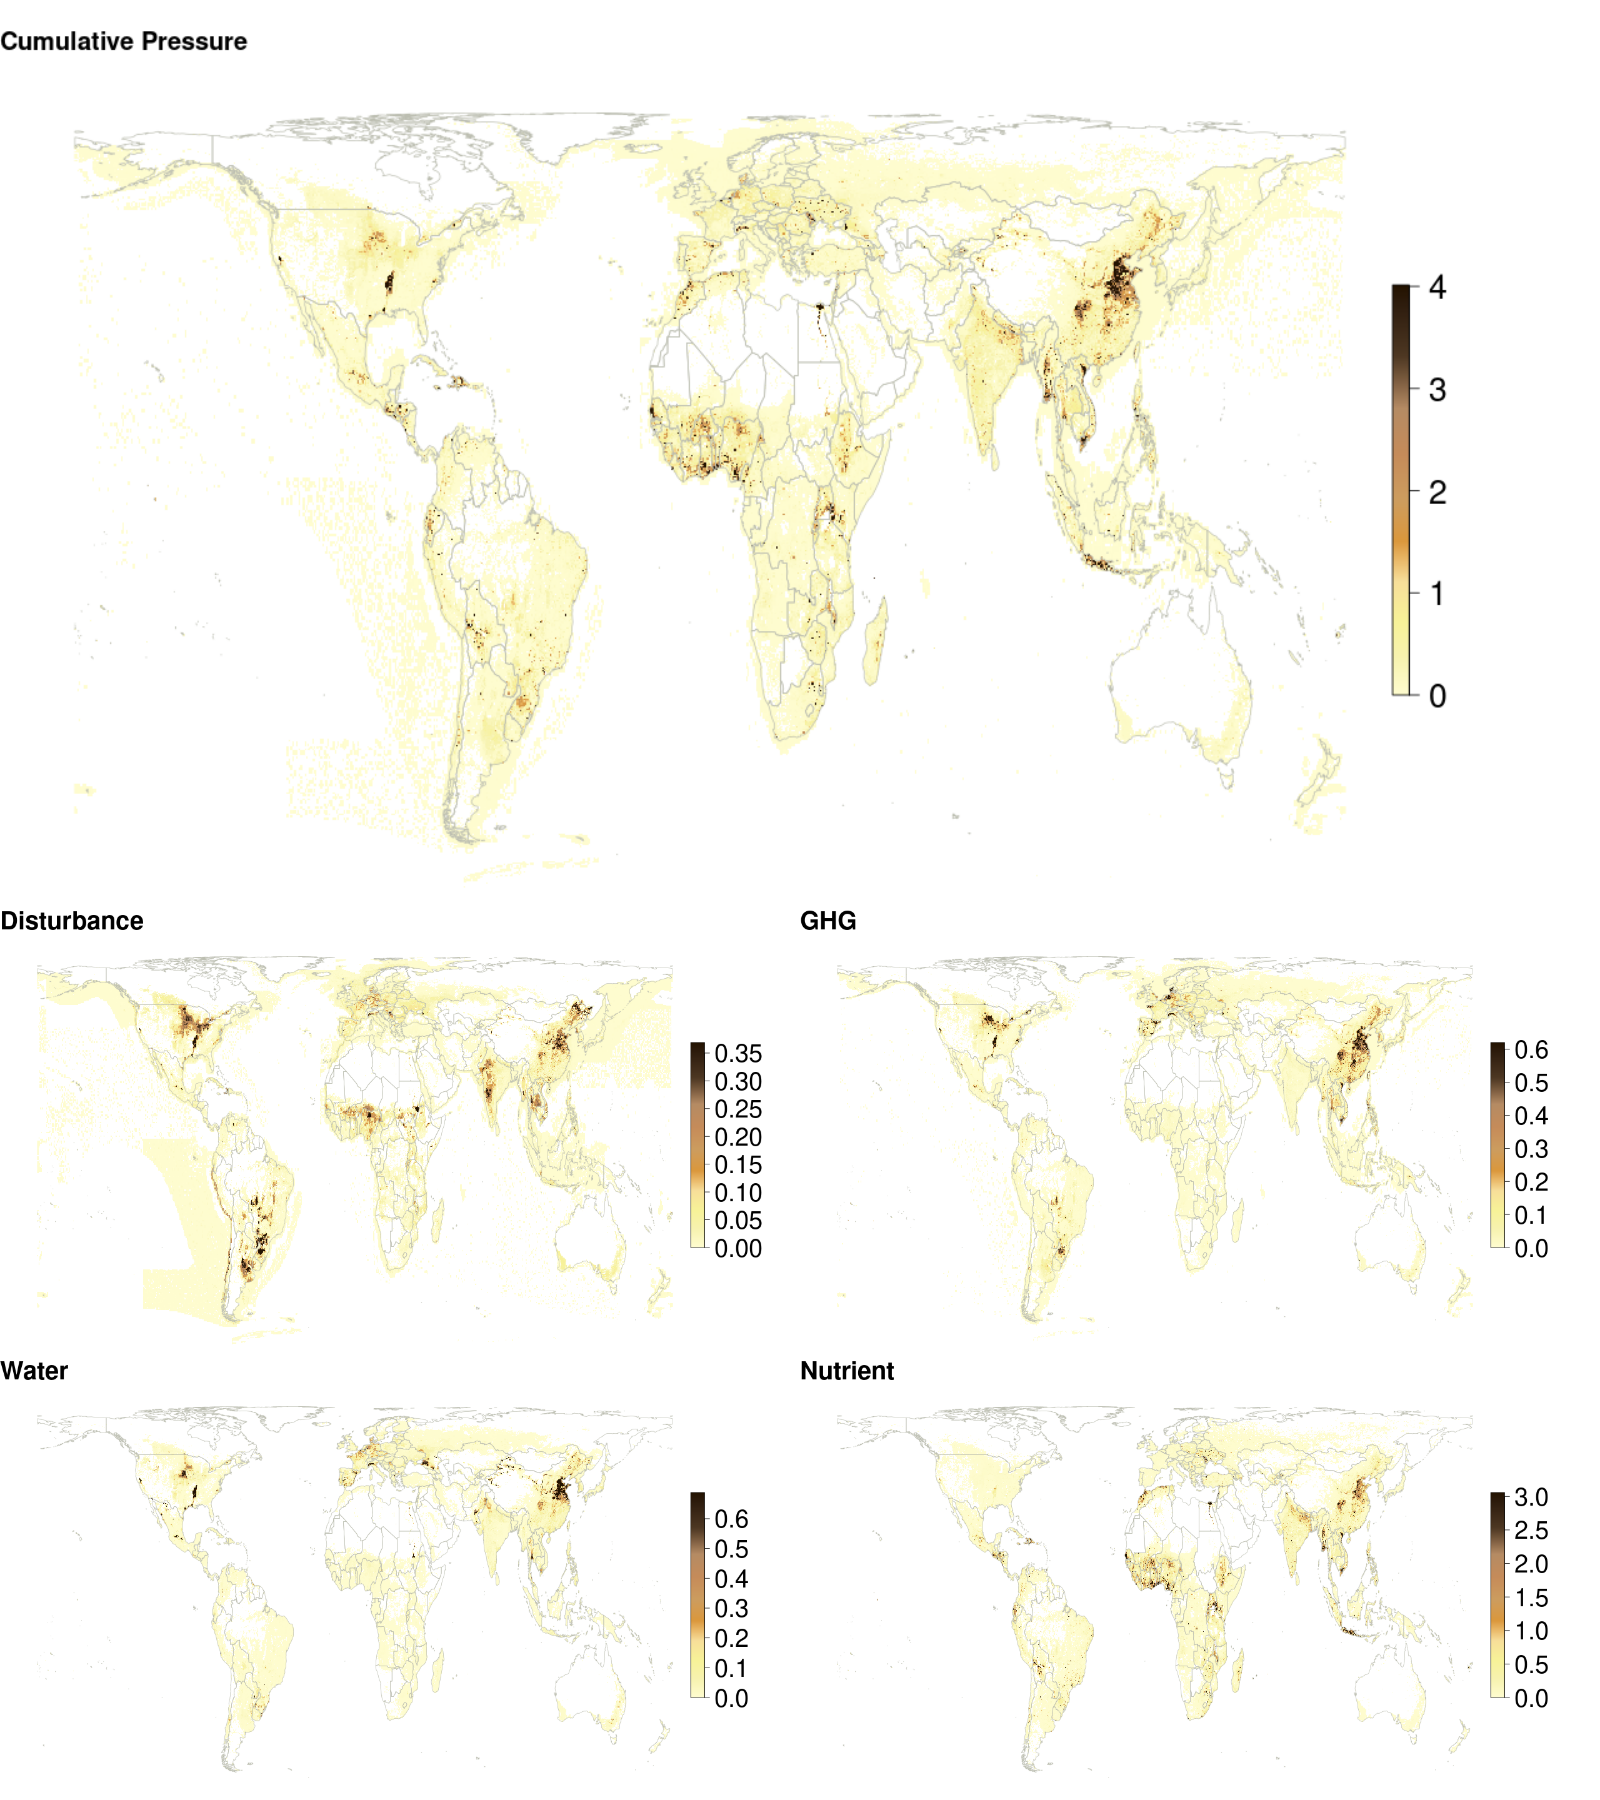
\includegraphics{/home/rayner/food-systems/_analysis/figures/extended_data/output/ed_fig_1_png/pigs_meat_final.png}

\begin{center}\rule{0.5\linewidth}{0.5pt}\end{center}

\hypertarget{sheep-meat}{%
\subparagraph{10) Sheep meat}\label{sheep-meat}}

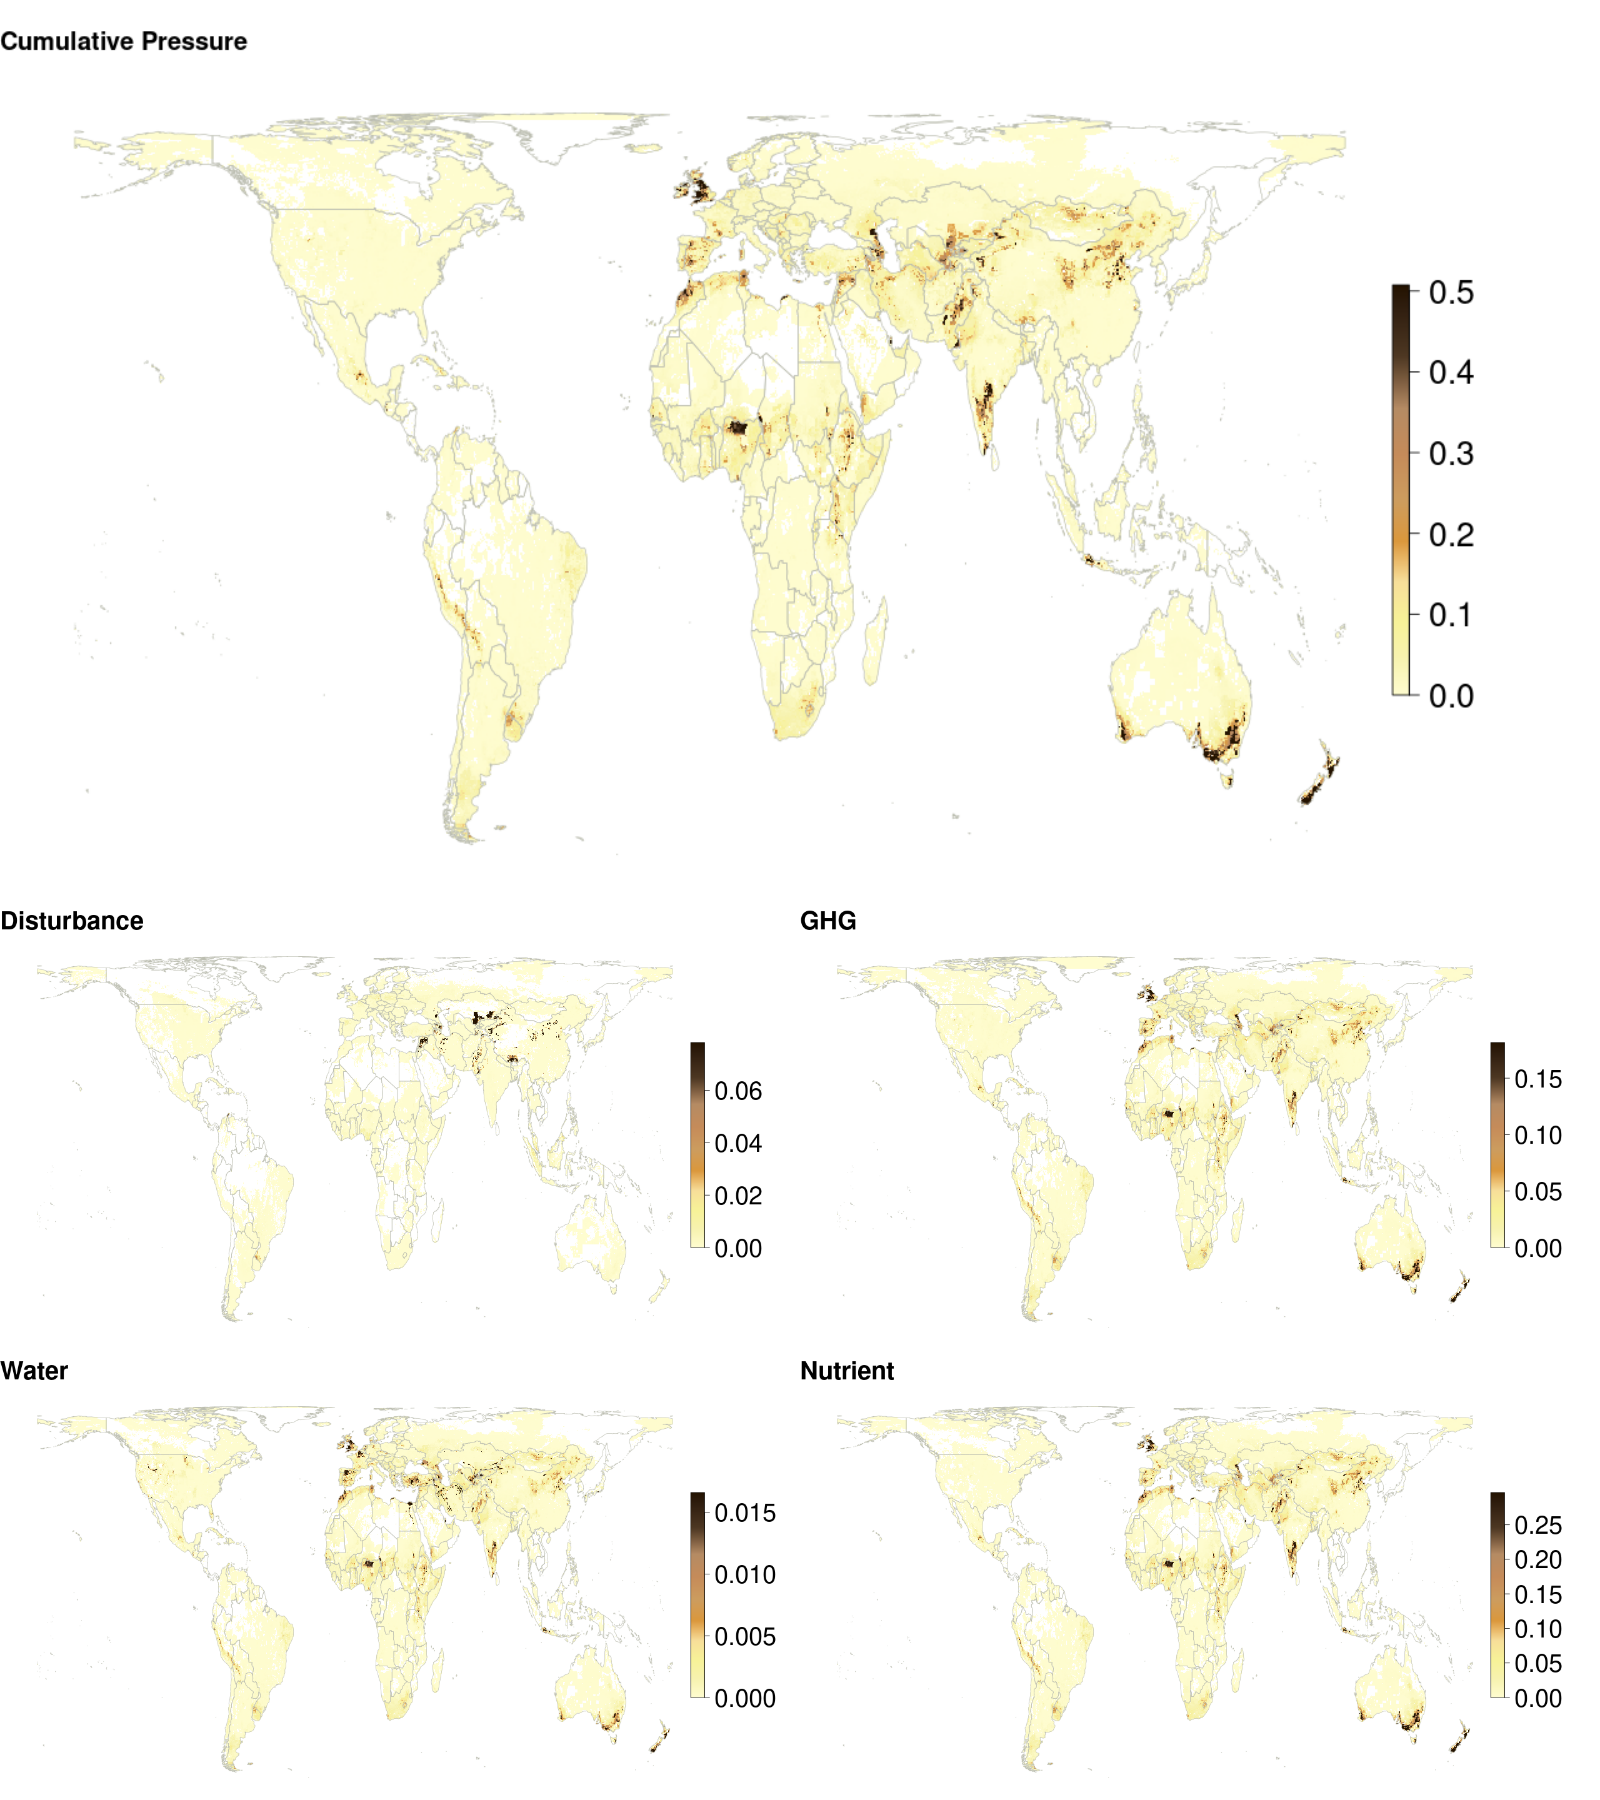
\includegraphics{/home/rayner/food-systems/_analysis/figures/extended_data/output/ed_fig_1_png/sheep_meat_final.png}

\begin{center}\rule{0.5\linewidth}{0.5pt}\end{center}

\hypertarget{sheep-milk}{%
\subparagraph{11) Sheep milk}\label{sheep-milk}}

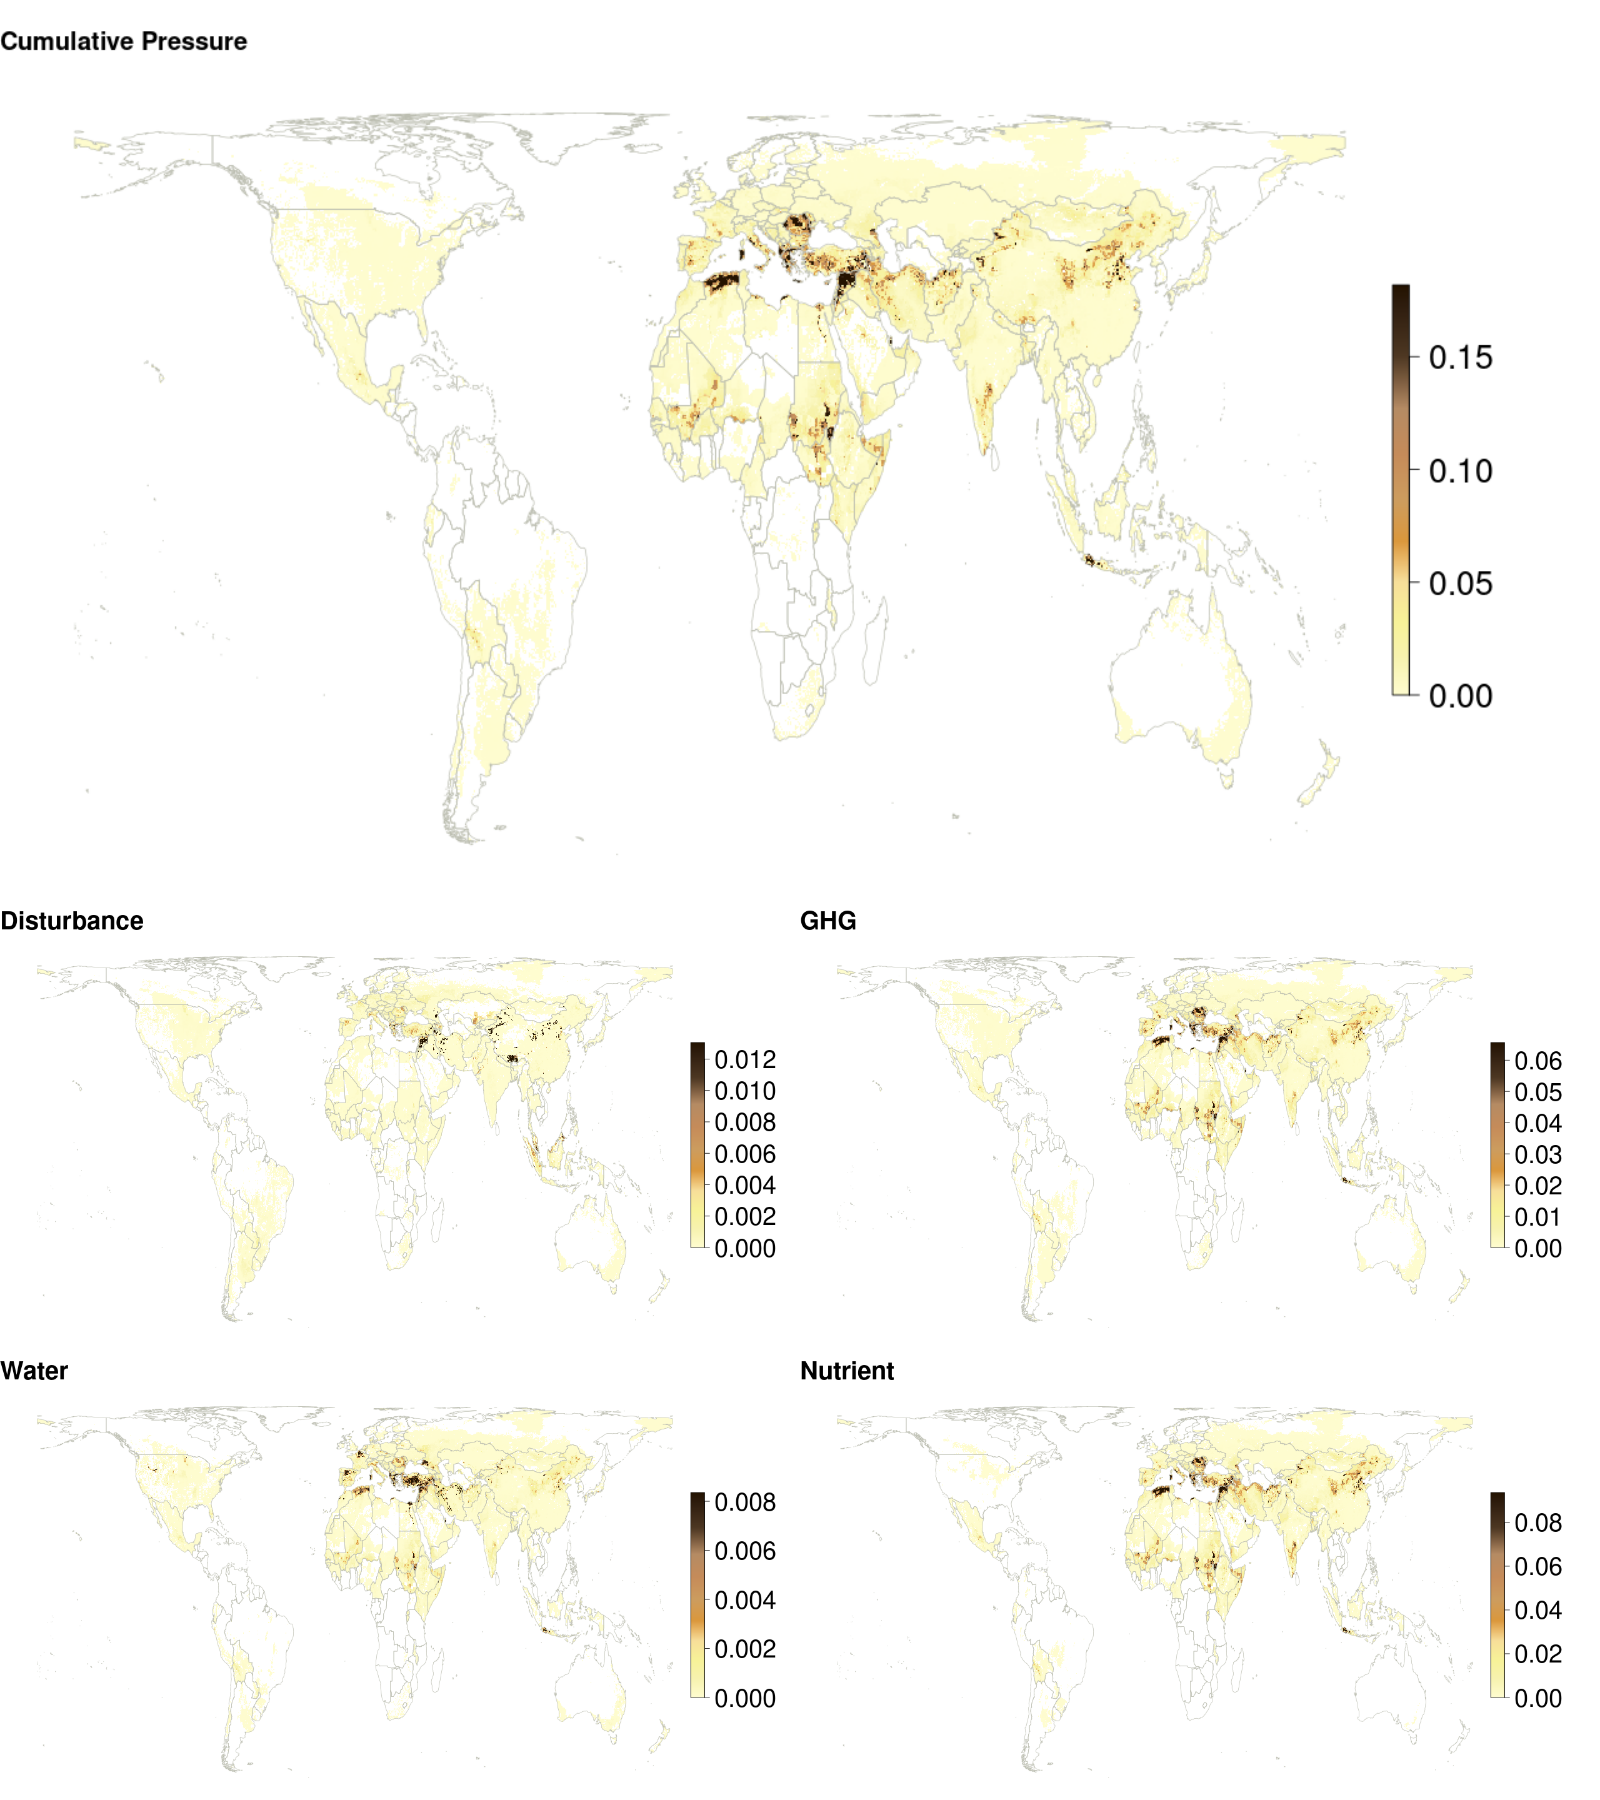
\includegraphics{/home/rayner/food-systems/_analysis/figures/extended_data/output/ed_fig_1_png/sheep_milk_final.png}

\begin{center}\rule{0.5\linewidth}{0.5pt}\end{center}

\hypertarget{extended-data-fig.-1c}{%
\paragraph{Extended Data Fig. 1c}\label{extended-data-fig.-1c}}

\textbf{Capture fisheries pressure maps}

Cumulative and individual (disturbance, GHG, water, nutrient) pressures
for seven categories of marine fisheries and one category of freshwater
fisheries. The individual pressure maps describe the rescaled pressure
data, calculated by dividing each pixel value (e.g.,
m\textsuperscript{3} water consumption) by the total global pressure
across all food systems and pixels, such that each pixel describes its
proportional contribution to the global total for that pressure. These
values were then multiplied by one million to prevent artefacts from
small values. The cumulative pressure score was calculated by summing
the rescaled pressure layers. Colour ramp scaling is unique to each plot
so the relative spatial distribution of each food item can be more
easily visualised.

\begin{center}\rule{0.5\linewidth}{0.5pt}\end{center}

\hypertarget{marine-benthic-fisheries}{%
\subparagraph{1) Marine benthic
fisheries}\label{marine-benthic-fisheries}}

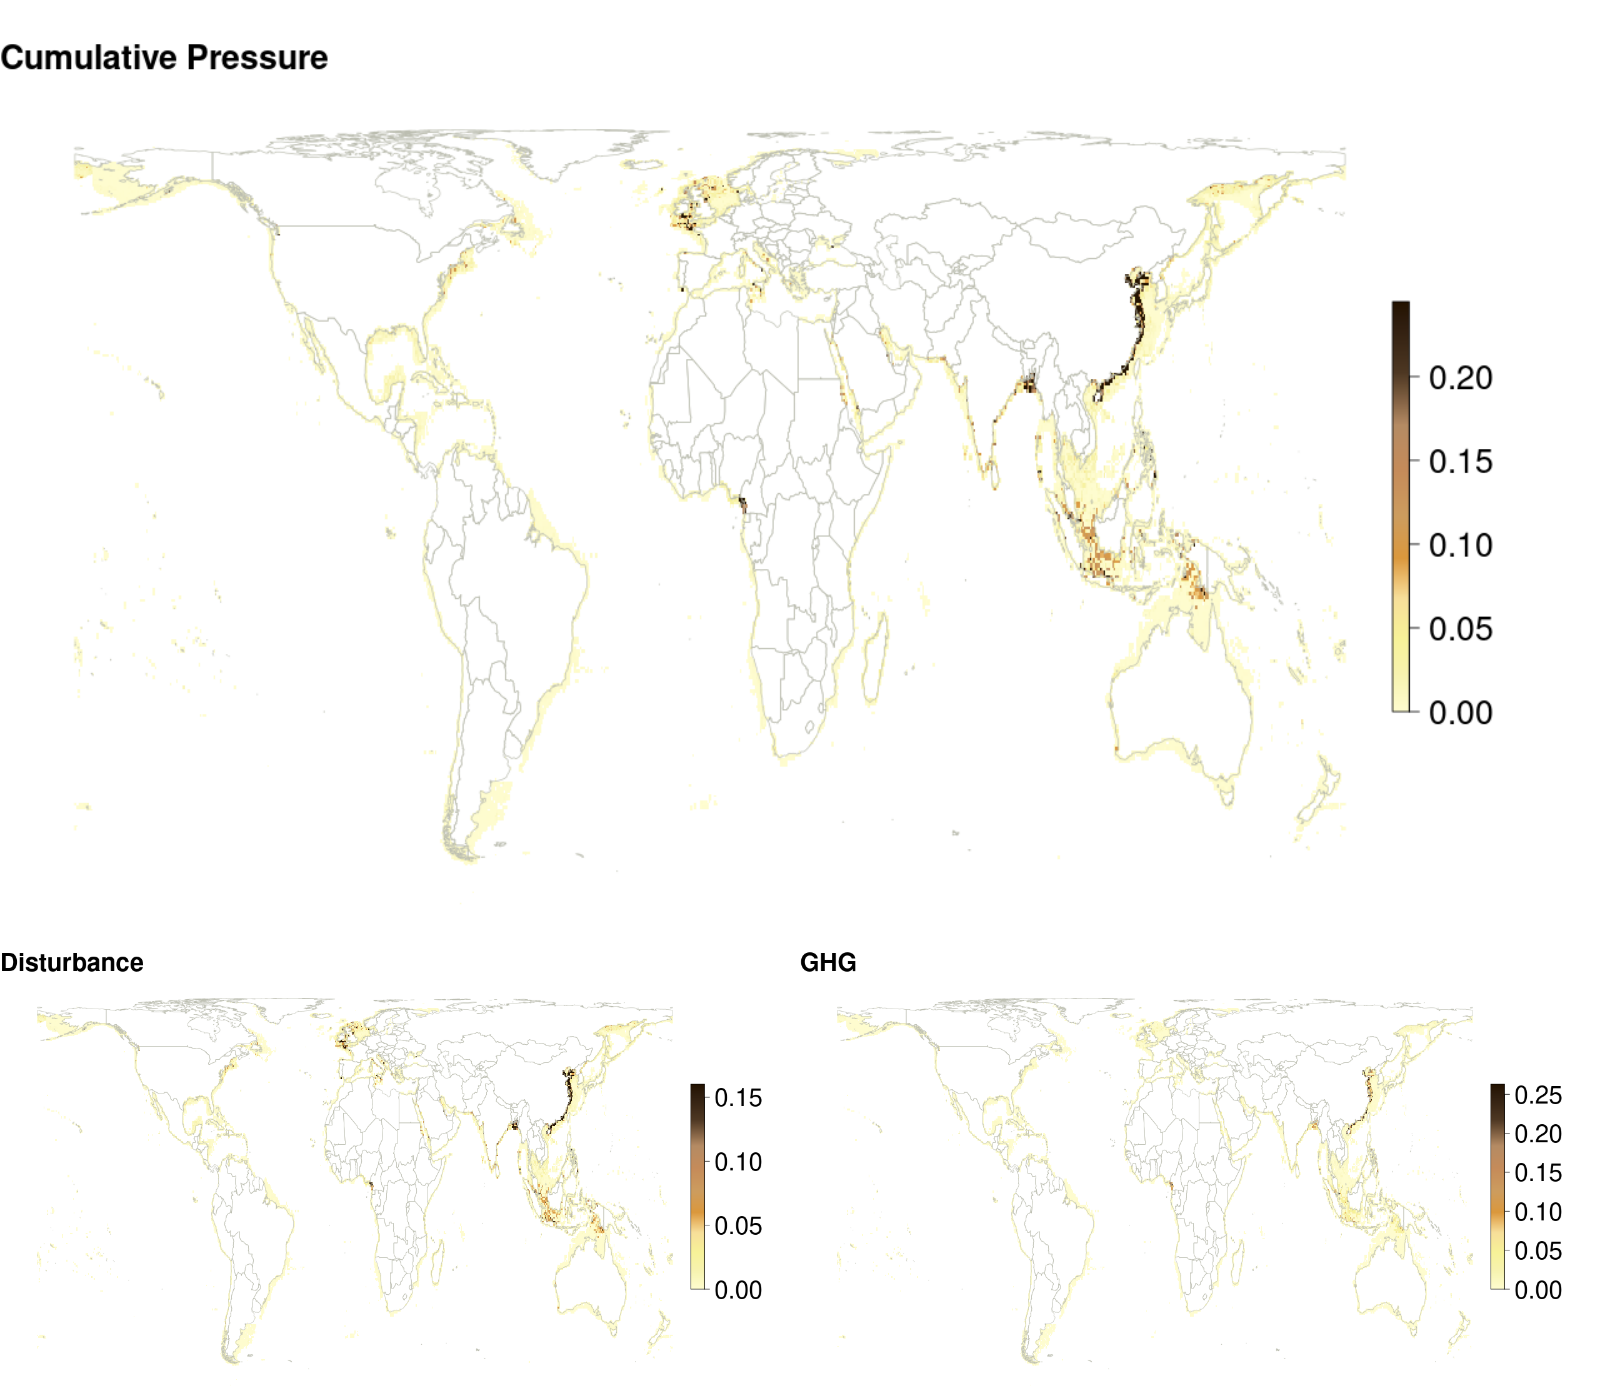
\includegraphics{/home/rayner/food-systems/_analysis/figures/extended_data/output/ed_fig_1_png/benthic_fisheries_final.png}

\begin{center}\rule{0.5\linewidth}{0.5pt}\end{center}

\hypertarget{marine-demersal-fisheries}{%
\subparagraph{2) Marine demersal
fisheries}\label{marine-demersal-fisheries}}

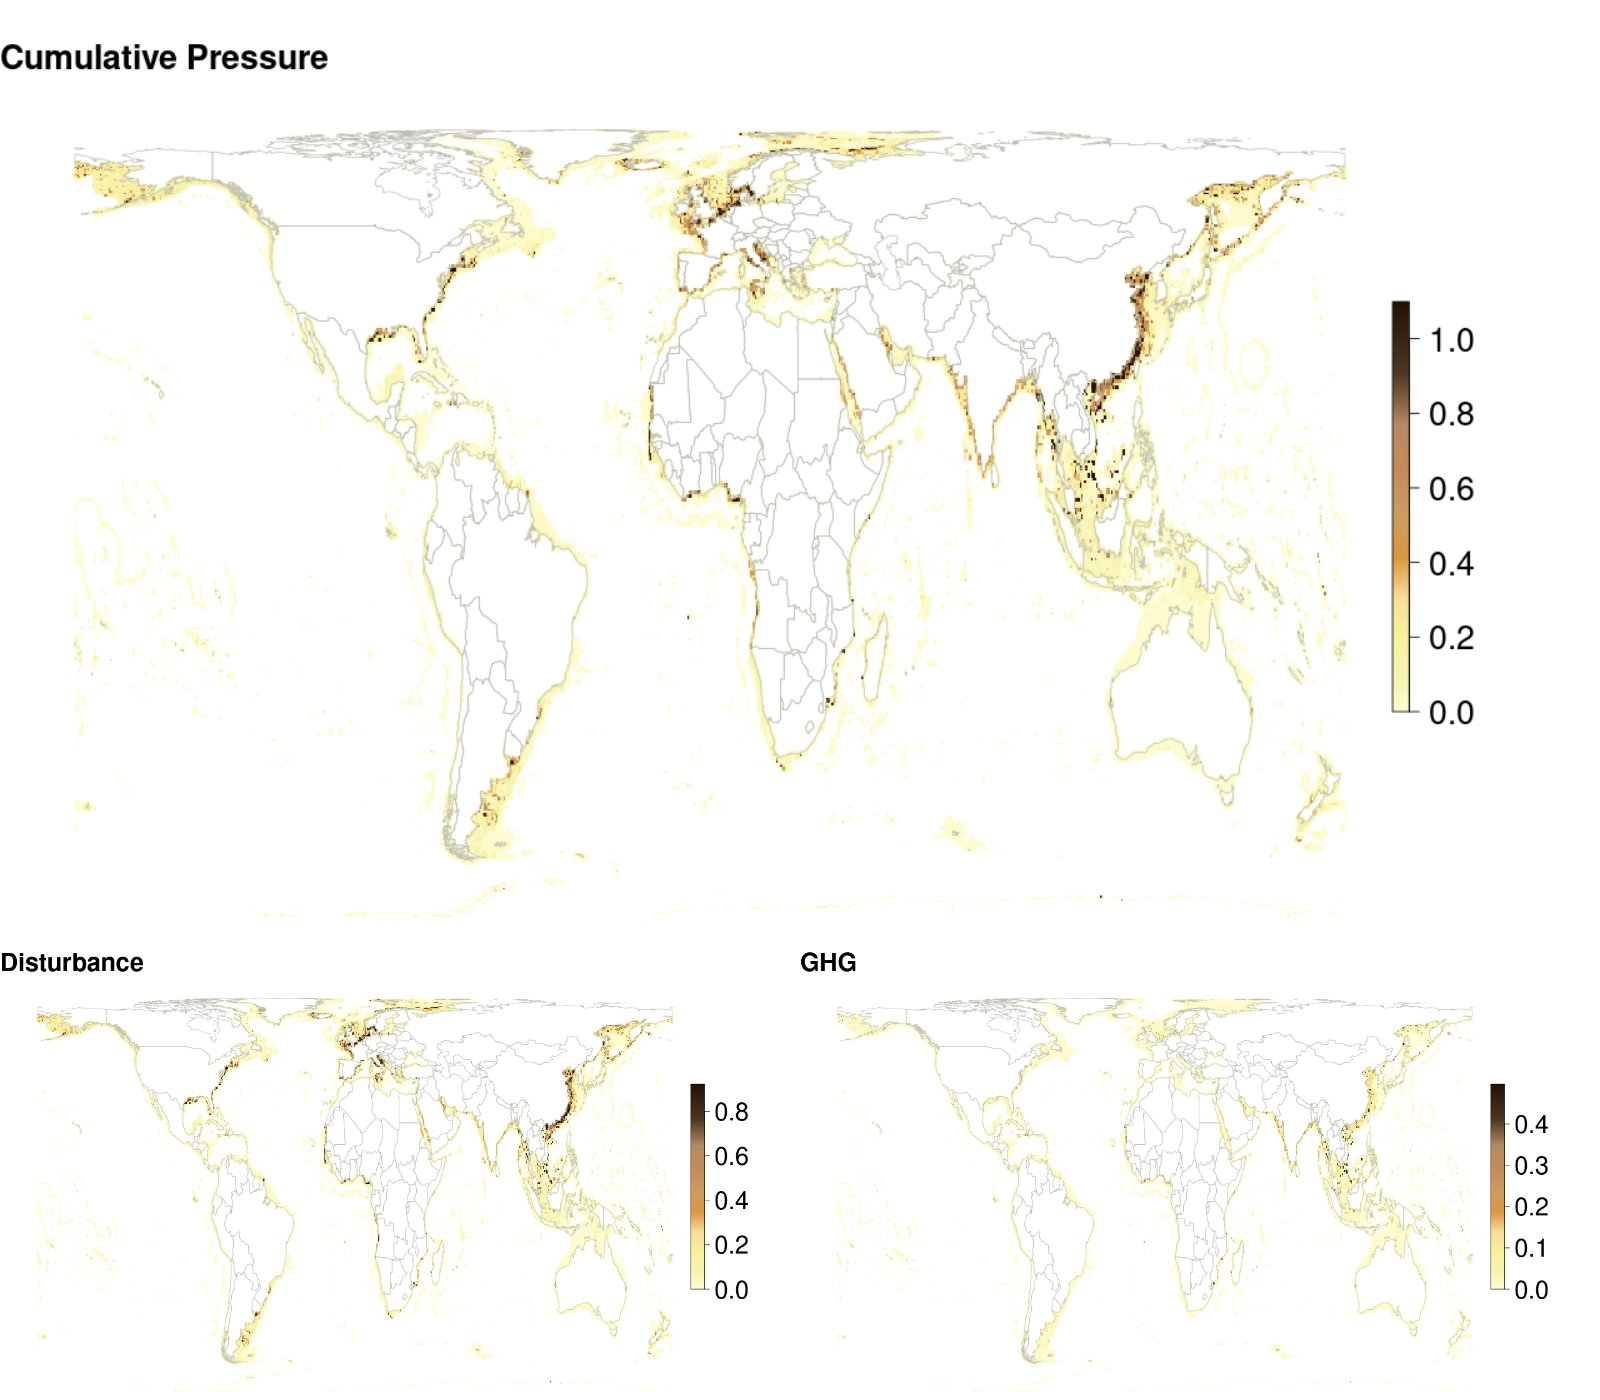
\includegraphics{/home/rayner/food-systems/_analysis/figures/extended_data/output/ed_fig_1_png/demersal_fisheries_final.png}

\begin{center}\rule{0.5\linewidth}{0.5pt}\end{center}

\hypertarget{marine-fish-oil-fish-meal-fisheries}{%
\subparagraph{3) Marine fish oil fish meal
fisheries}\label{marine-fish-oil-fish-meal-fisheries}}

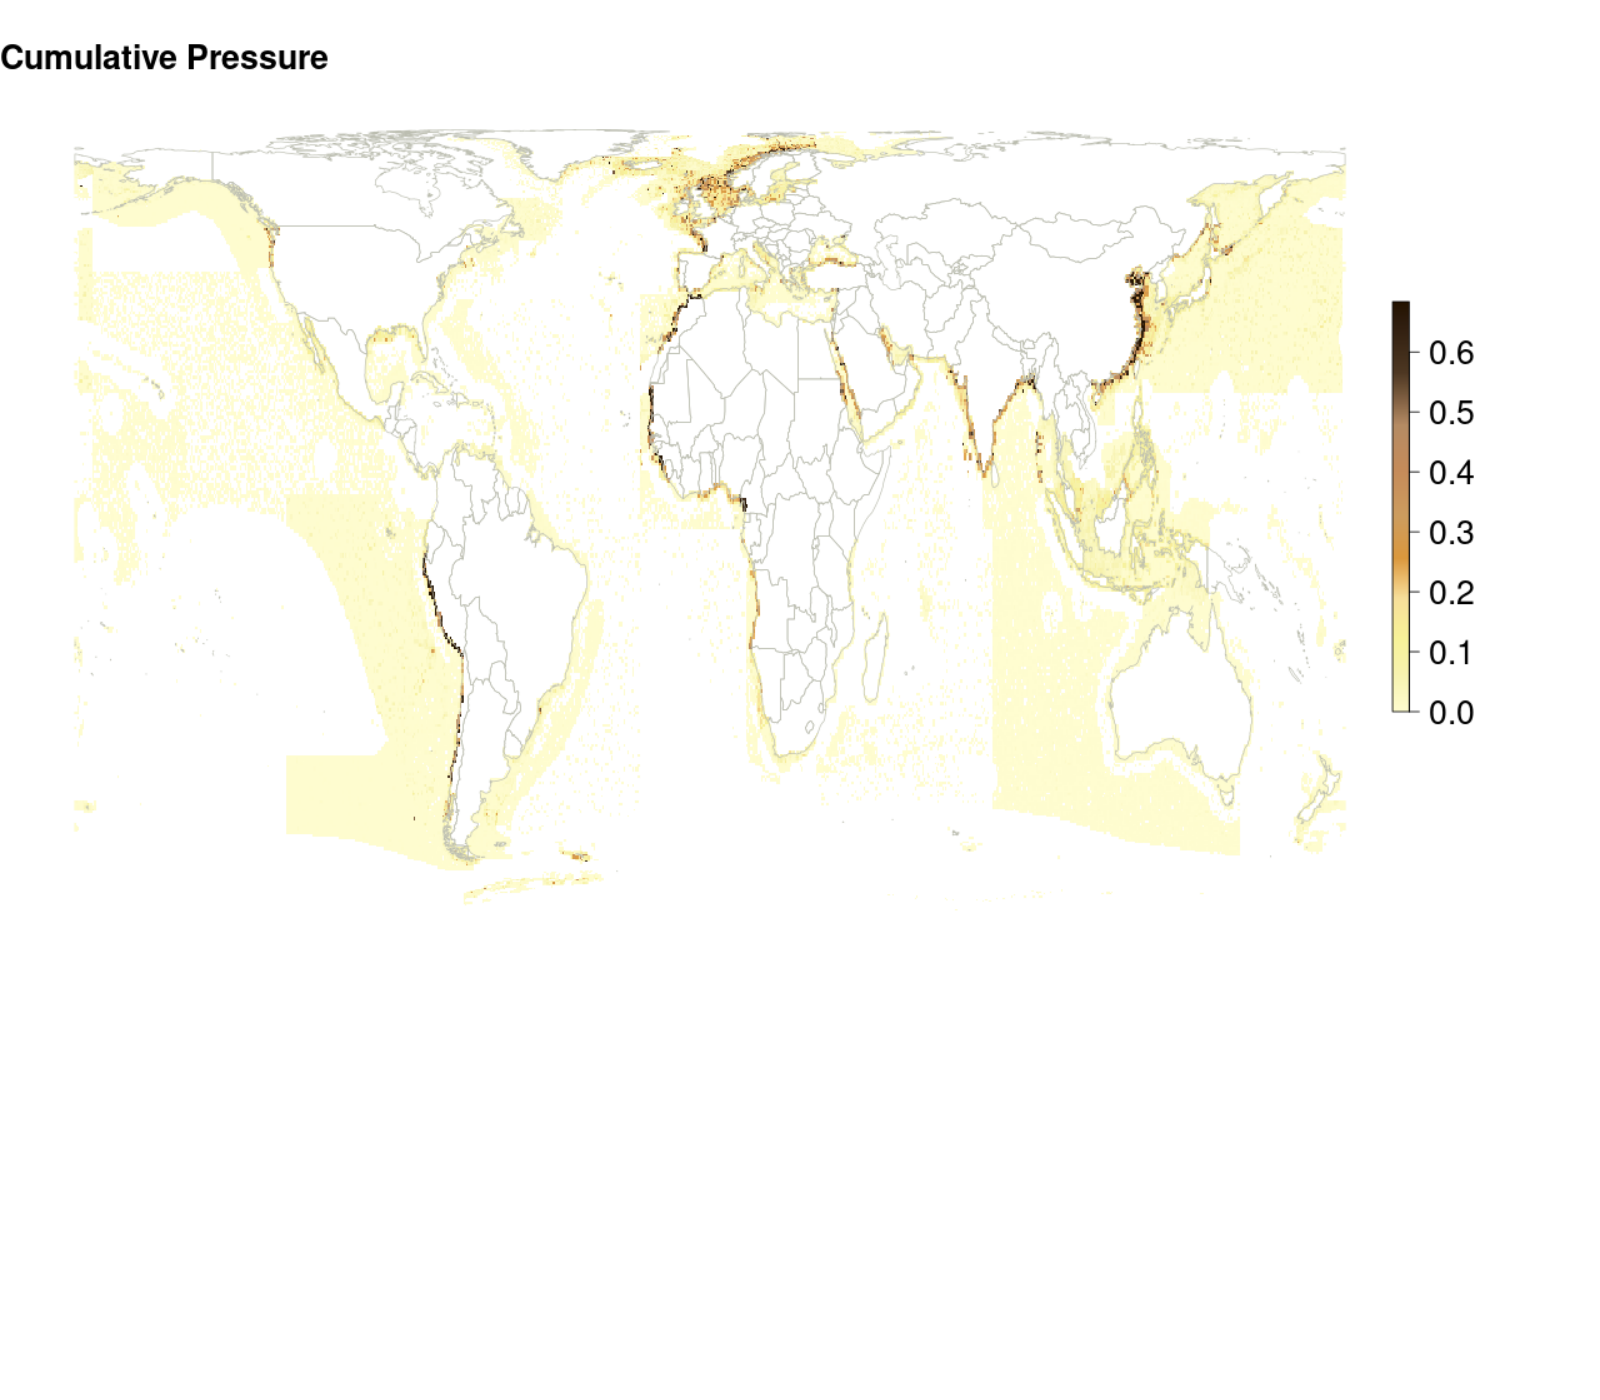
\includegraphics{/home/rayner/food-systems/_analysis/figures/extended_data/output/ed_fig_1_png/fofm_fisheries_final.png}

\begin{center}\rule{0.5\linewidth}{0.5pt}\end{center}

\hypertarget{marine-large-pelagic-fisheries}{%
\subparagraph{4) Marine large pelagic
fisheries}\label{marine-large-pelagic-fisheries}}

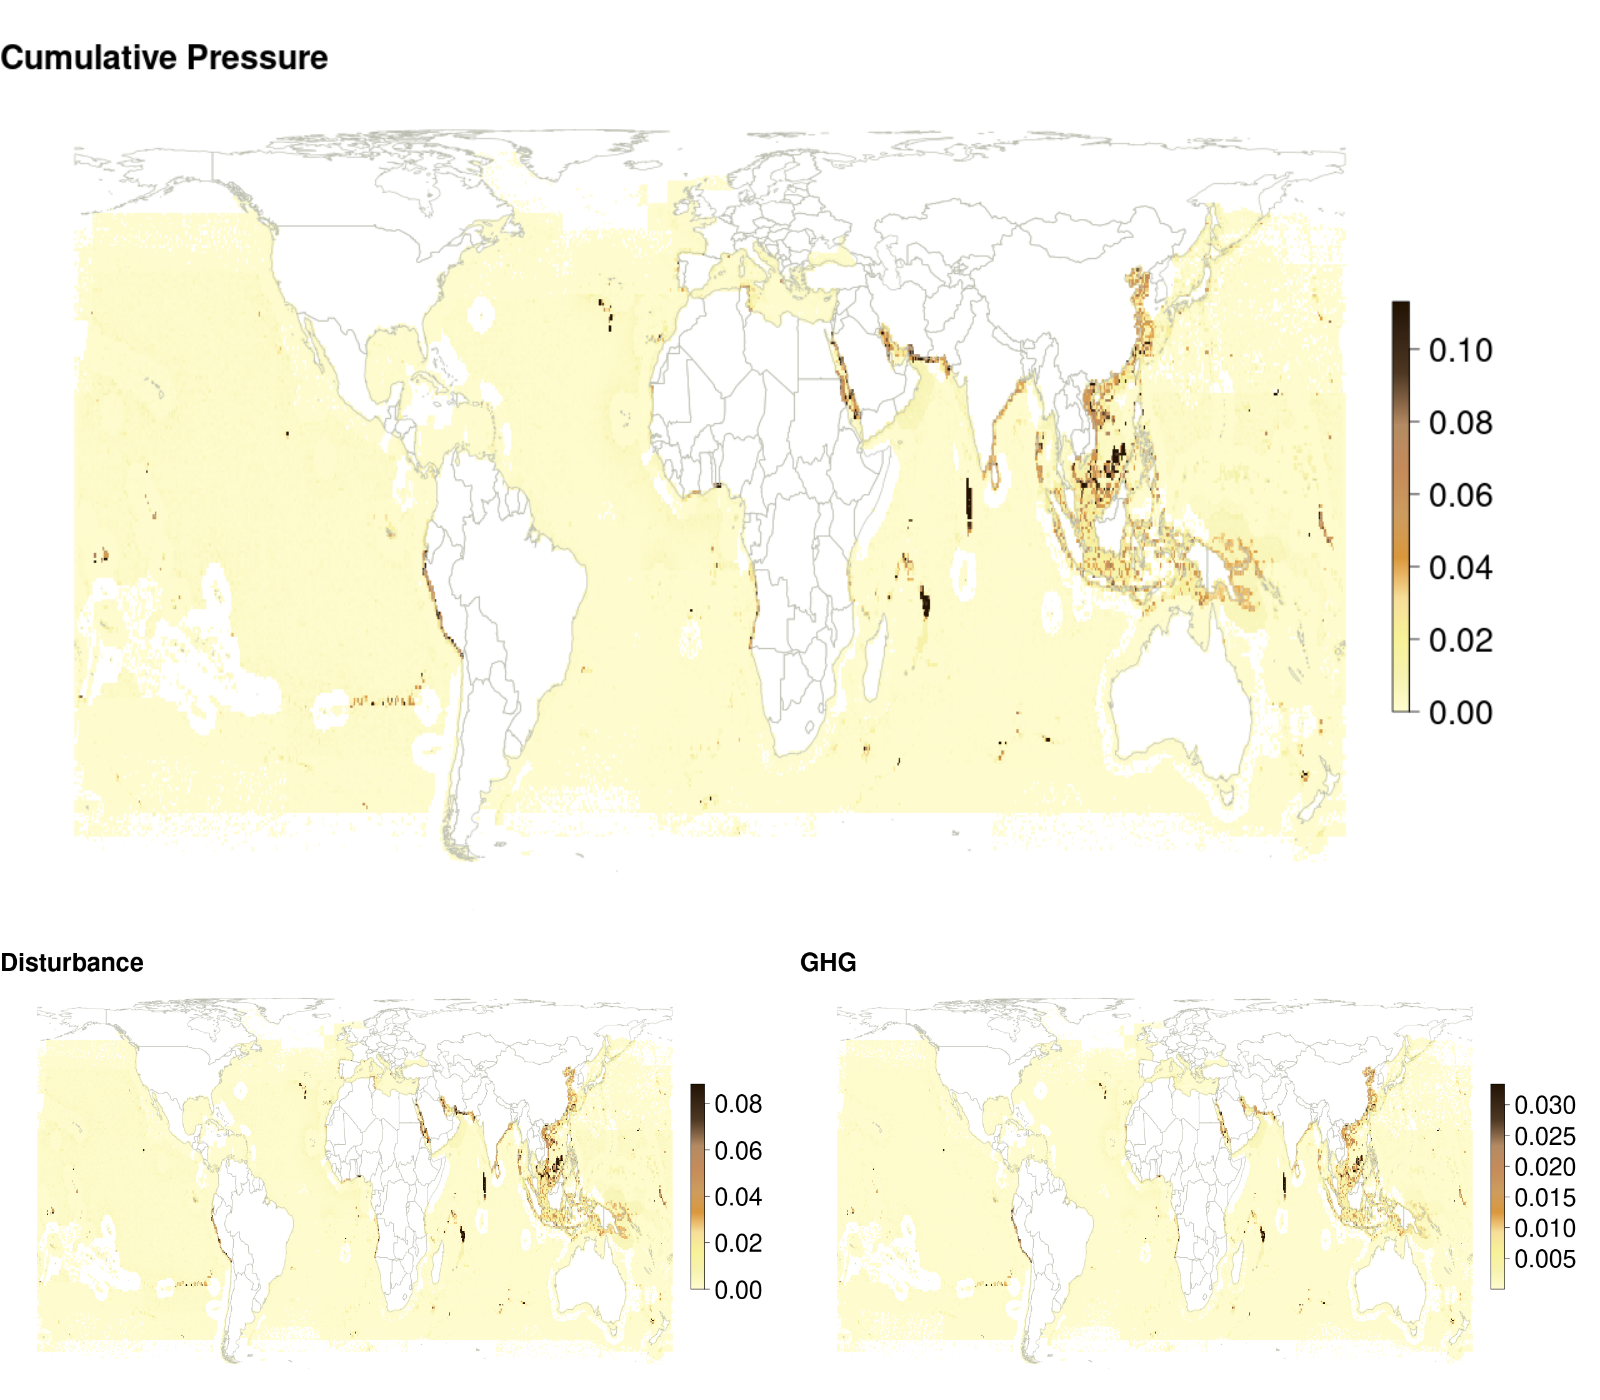
\includegraphics{/home/rayner/food-systems/_analysis/figures/extended_data/output/ed_fig_1_png/large-pelagic_fisheries_final.png}

\begin{center}\rule{0.5\linewidth}{0.5pt}\end{center}

\hypertarget{marine-medium-pelagic-fisheries}{%
\subparagraph{5) Marine medium pelagic
fisheries}\label{marine-medium-pelagic-fisheries}}

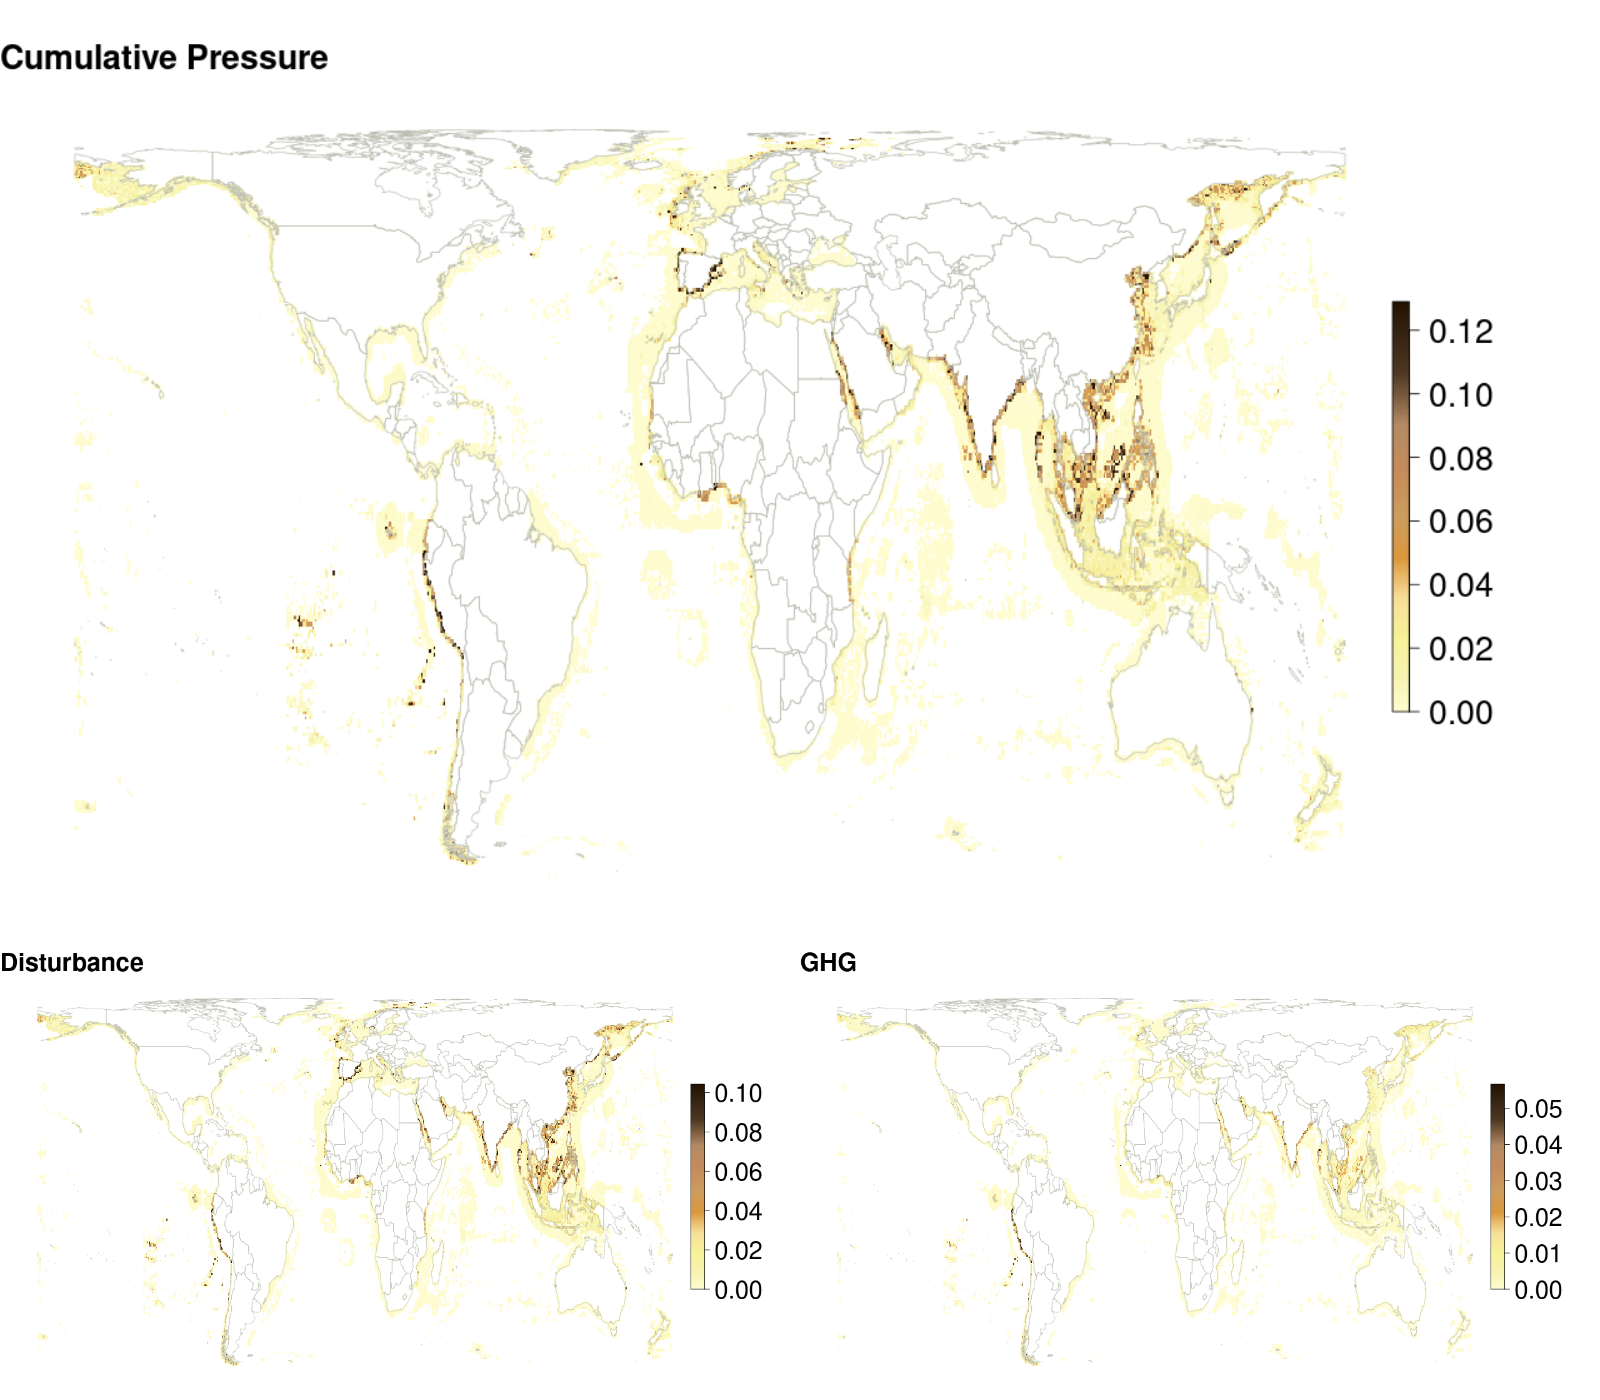
\includegraphics{/home/rayner/food-systems/_analysis/figures/extended_data/output/ed_fig_1_png/medium-pelagic_fisheries_final.png}

\begin{center}\rule{0.5\linewidth}{0.5pt}\end{center}

\hypertarget{marine-reef-fisheries}{%
\subparagraph{6) Marine reef fisheries}\label{marine-reef-fisheries}}

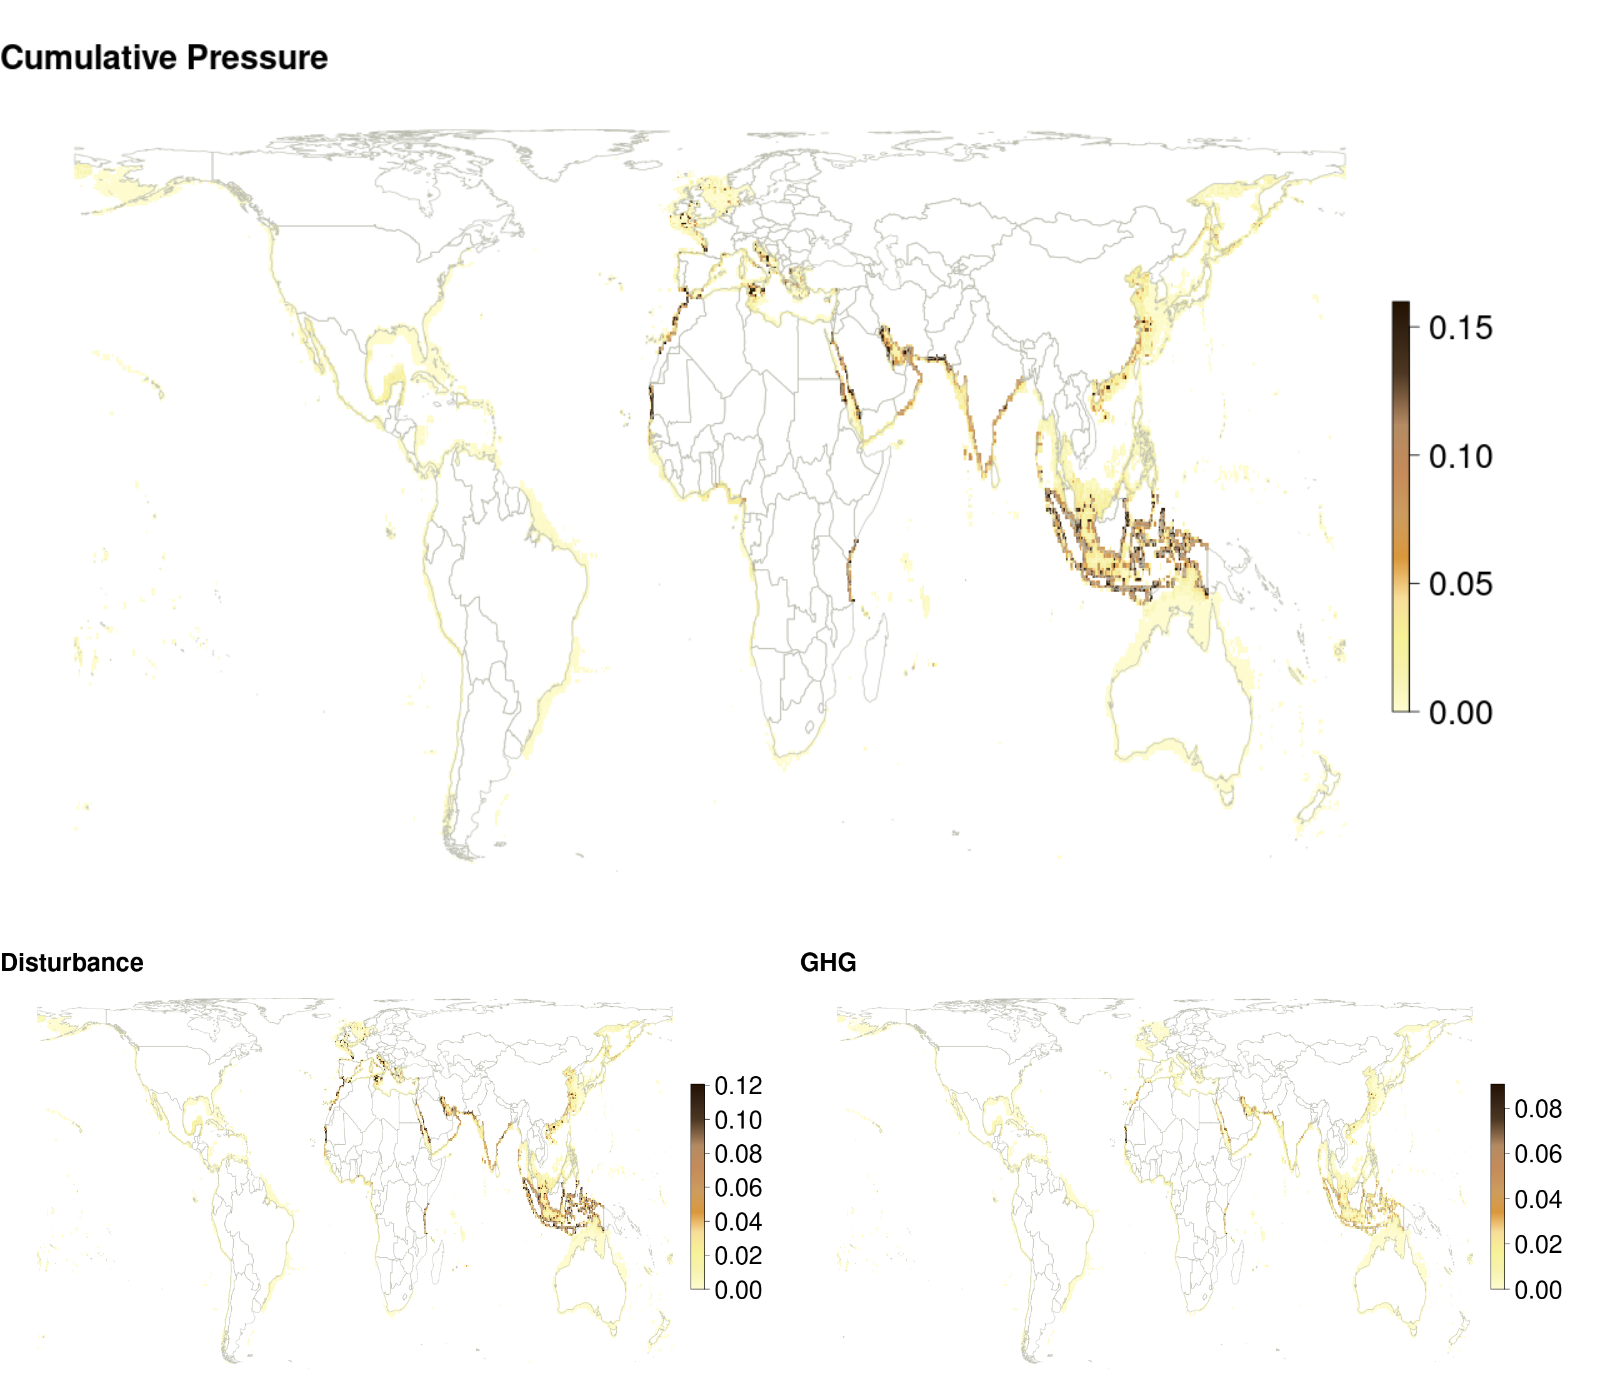
\includegraphics{/home/rayner/food-systems/_analysis/figures/extended_data/output/ed_fig_1_png/reef_fisheries_final.png}

\begin{center}\rule{0.5\linewidth}{0.5pt}\end{center}

\hypertarget{marine-small-pelagic-fisheries}{%
\subparagraph{7) Marine small pelagic
fisheries}\label{marine-small-pelagic-fisheries}}

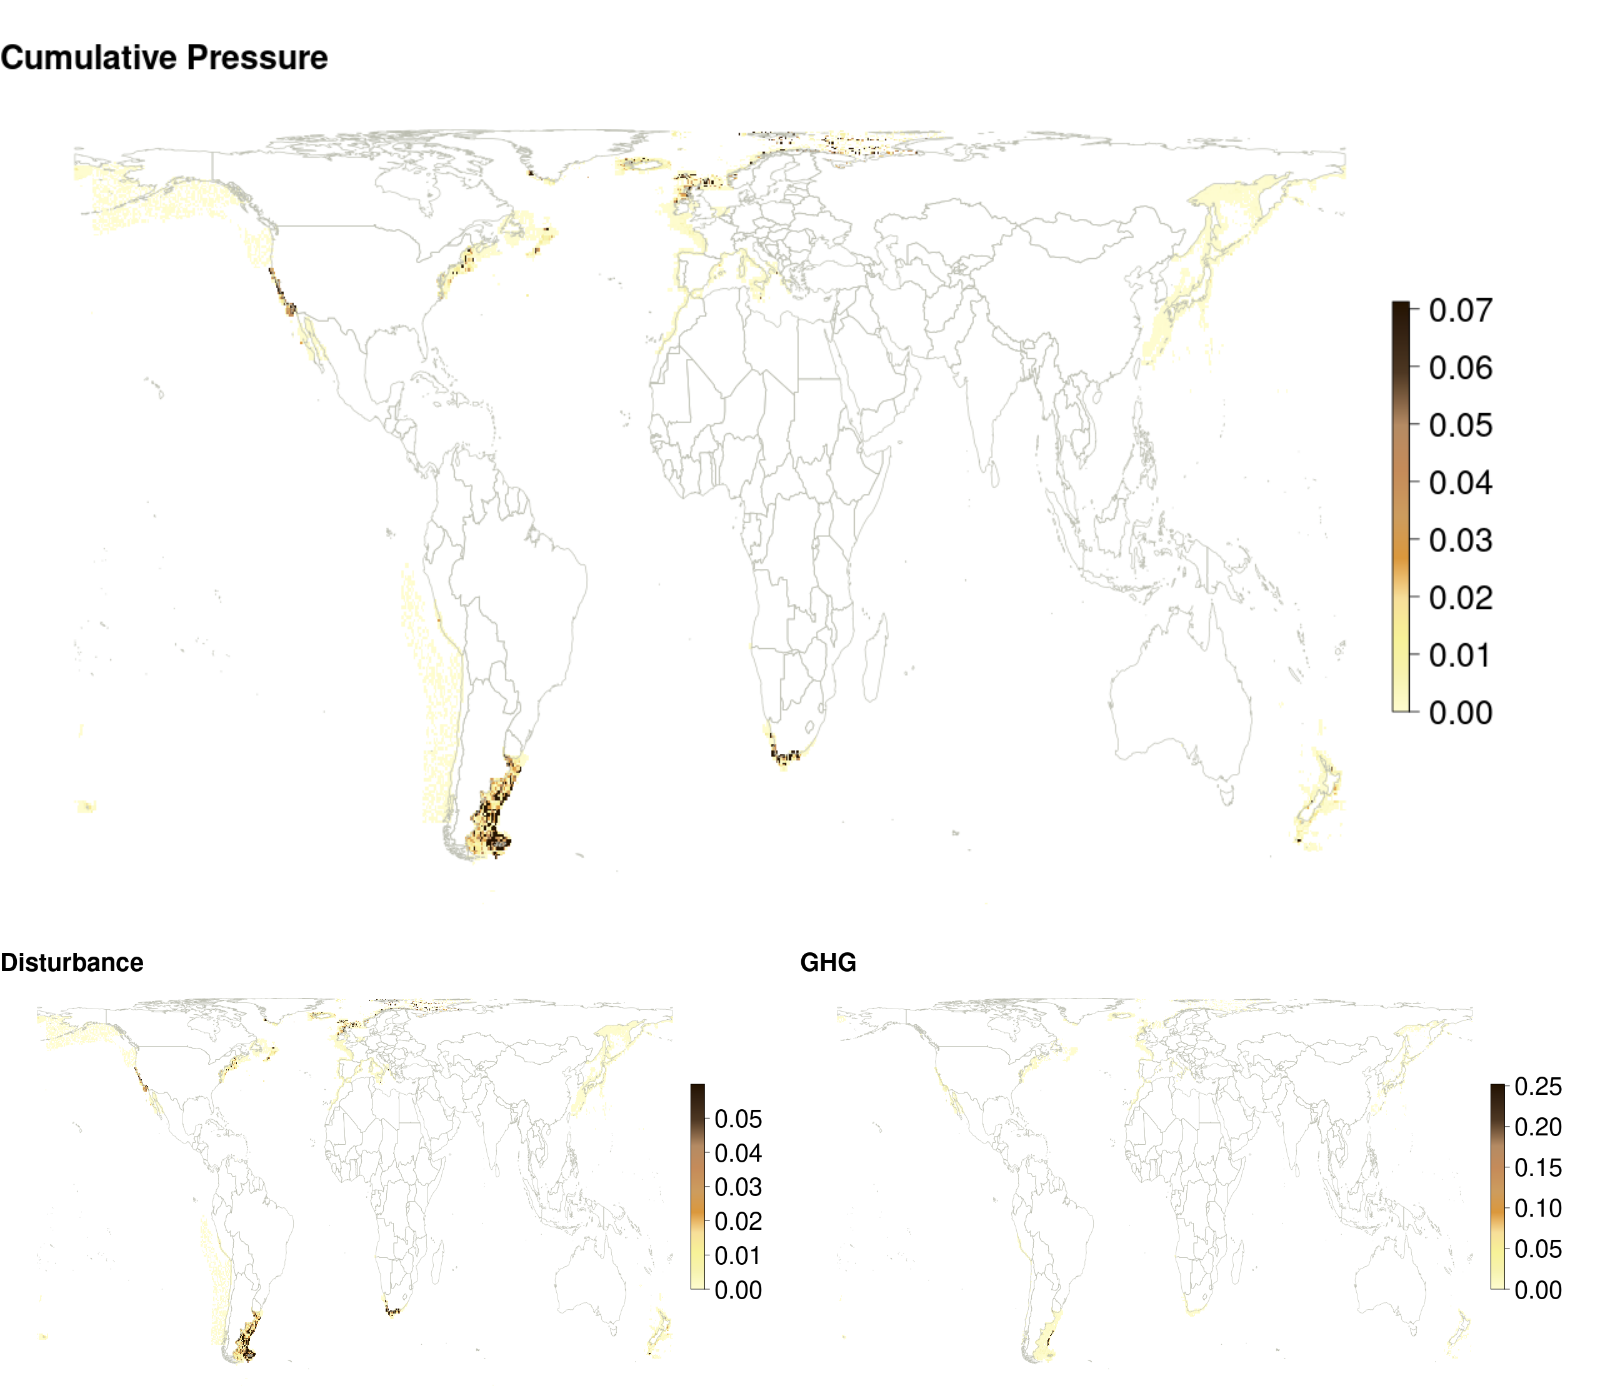
\includegraphics{/home/rayner/food-systems/_analysis/figures/extended_data/output/ed_fig_1_png/small-pelagic_fisheries_final.png}

\begin{center}\rule{0.5\linewidth}{0.5pt}\end{center}

\hypertarget{freshwater-fisheries}{%
\subparagraph{8) Freshwater fisheries}\label{freshwater-fisheries}}

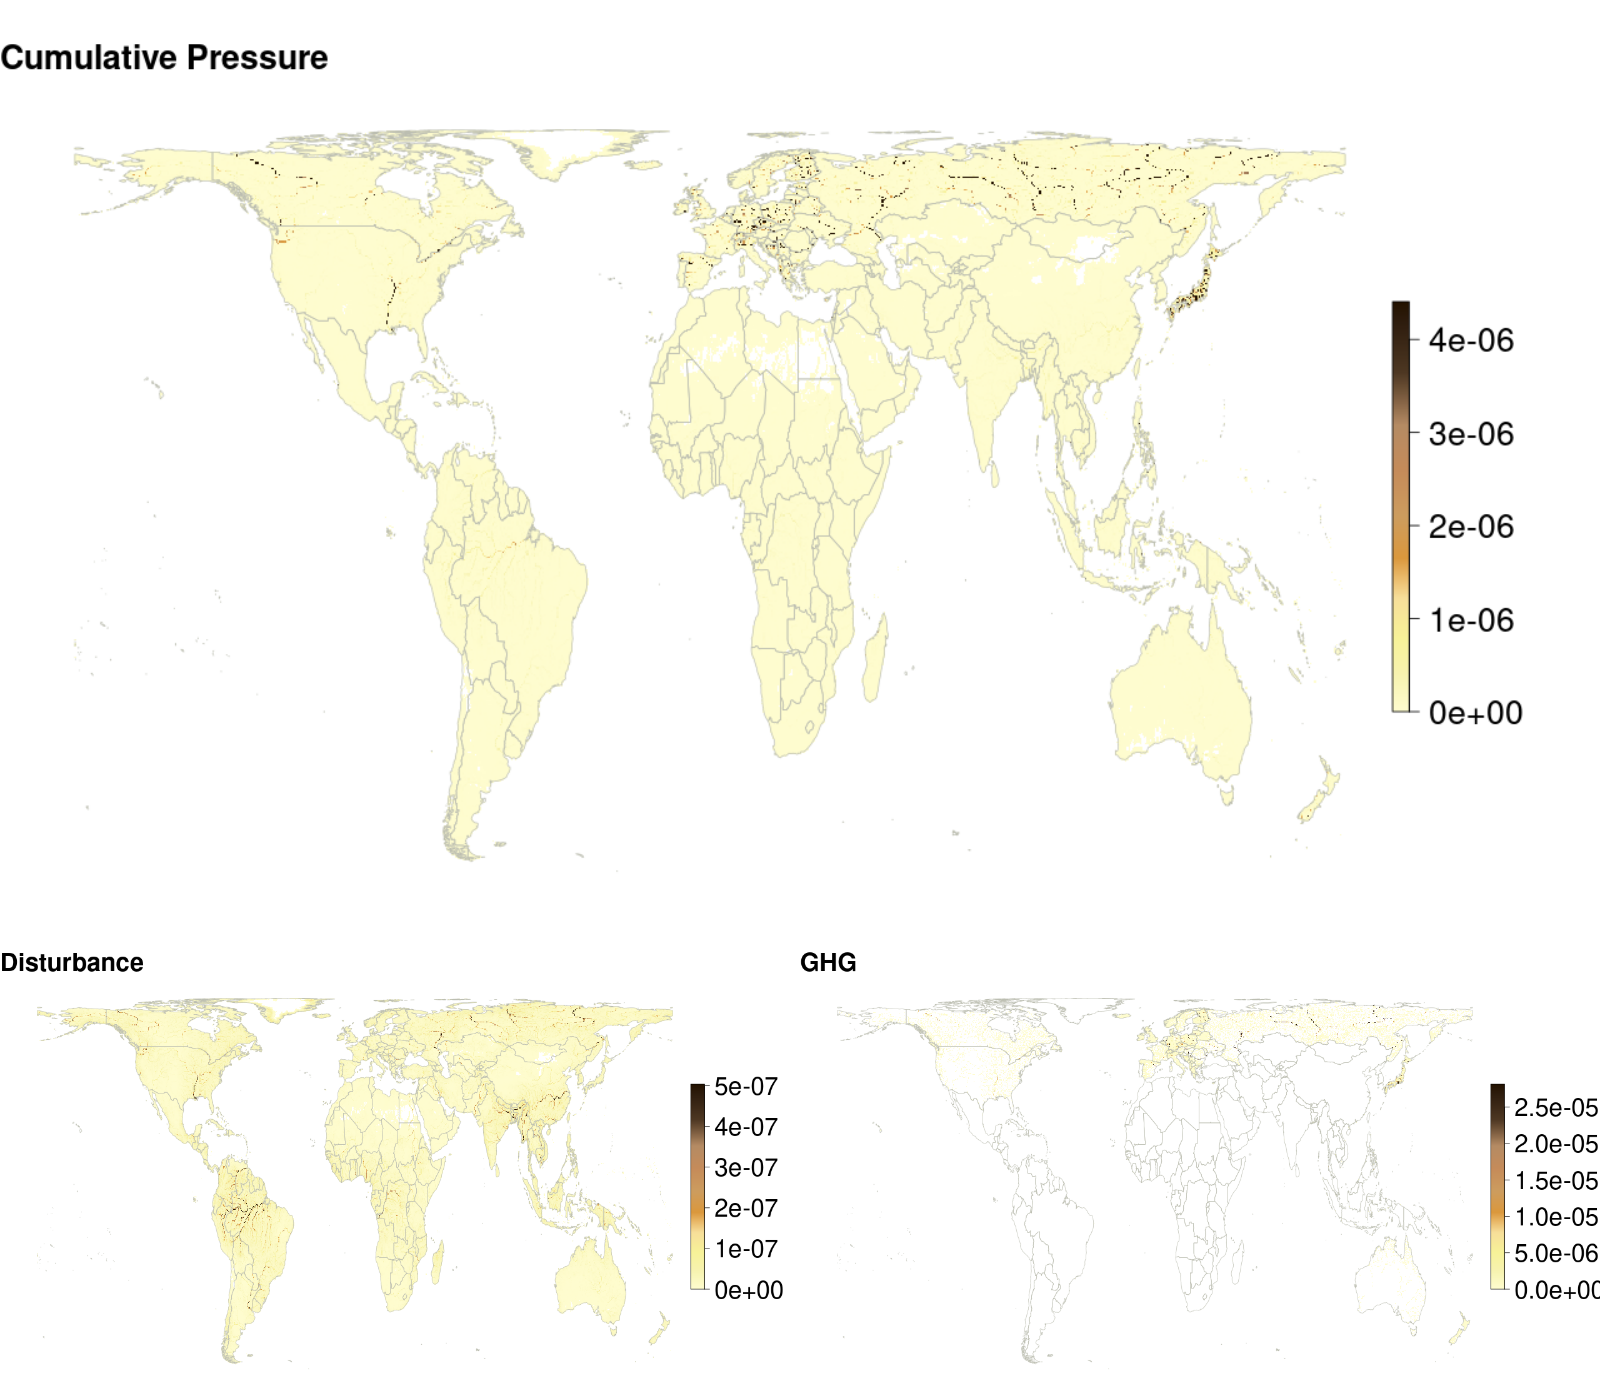
\includegraphics{/home/rayner/food-systems/_analysis/figures/extended_data/output/ed_fig_1_png/wildcaught_freshwater_final.png}

\begin{center}\rule{0.5\linewidth}{0.5pt}\end{center}

\hypertarget{extended-data-fig.-1d}{%
\paragraph{Extended Data Fig. 1d}\label{extended-data-fig.-1d}}

\textbf{Marine aquaculture pressure maps}

Cumulative and individual (disturbance, GHG, water, nutrient) pressures
for six categories of marine aquaculture. Data includes both on-farm
pressures and off-farm feed pressures (except for unfed or algae fed
shellfish). The individual pressure maps describe the rescaled pressure
data, calculated by dividing each pixel value (e.g.,
m\textsuperscript{3} water consumption) by the total global pressure
across all food systems and pixels, such that each pixel describes its
proportional contribution to the global total for that pressure. These
values were then multiplied by one million to prevent artefacts from
small values. The cumulative pressure score was calculated by summing
the rescaled pressure layers. Colour ramp scaling is unique to each plot
so the relative spatial distribution of each food item can be more
easily visualised.

\hypertarget{bivalve-aquaculture}{%
\subparagraph{1) Bivalve aquaculture}\label{bivalve-aquaculture}}

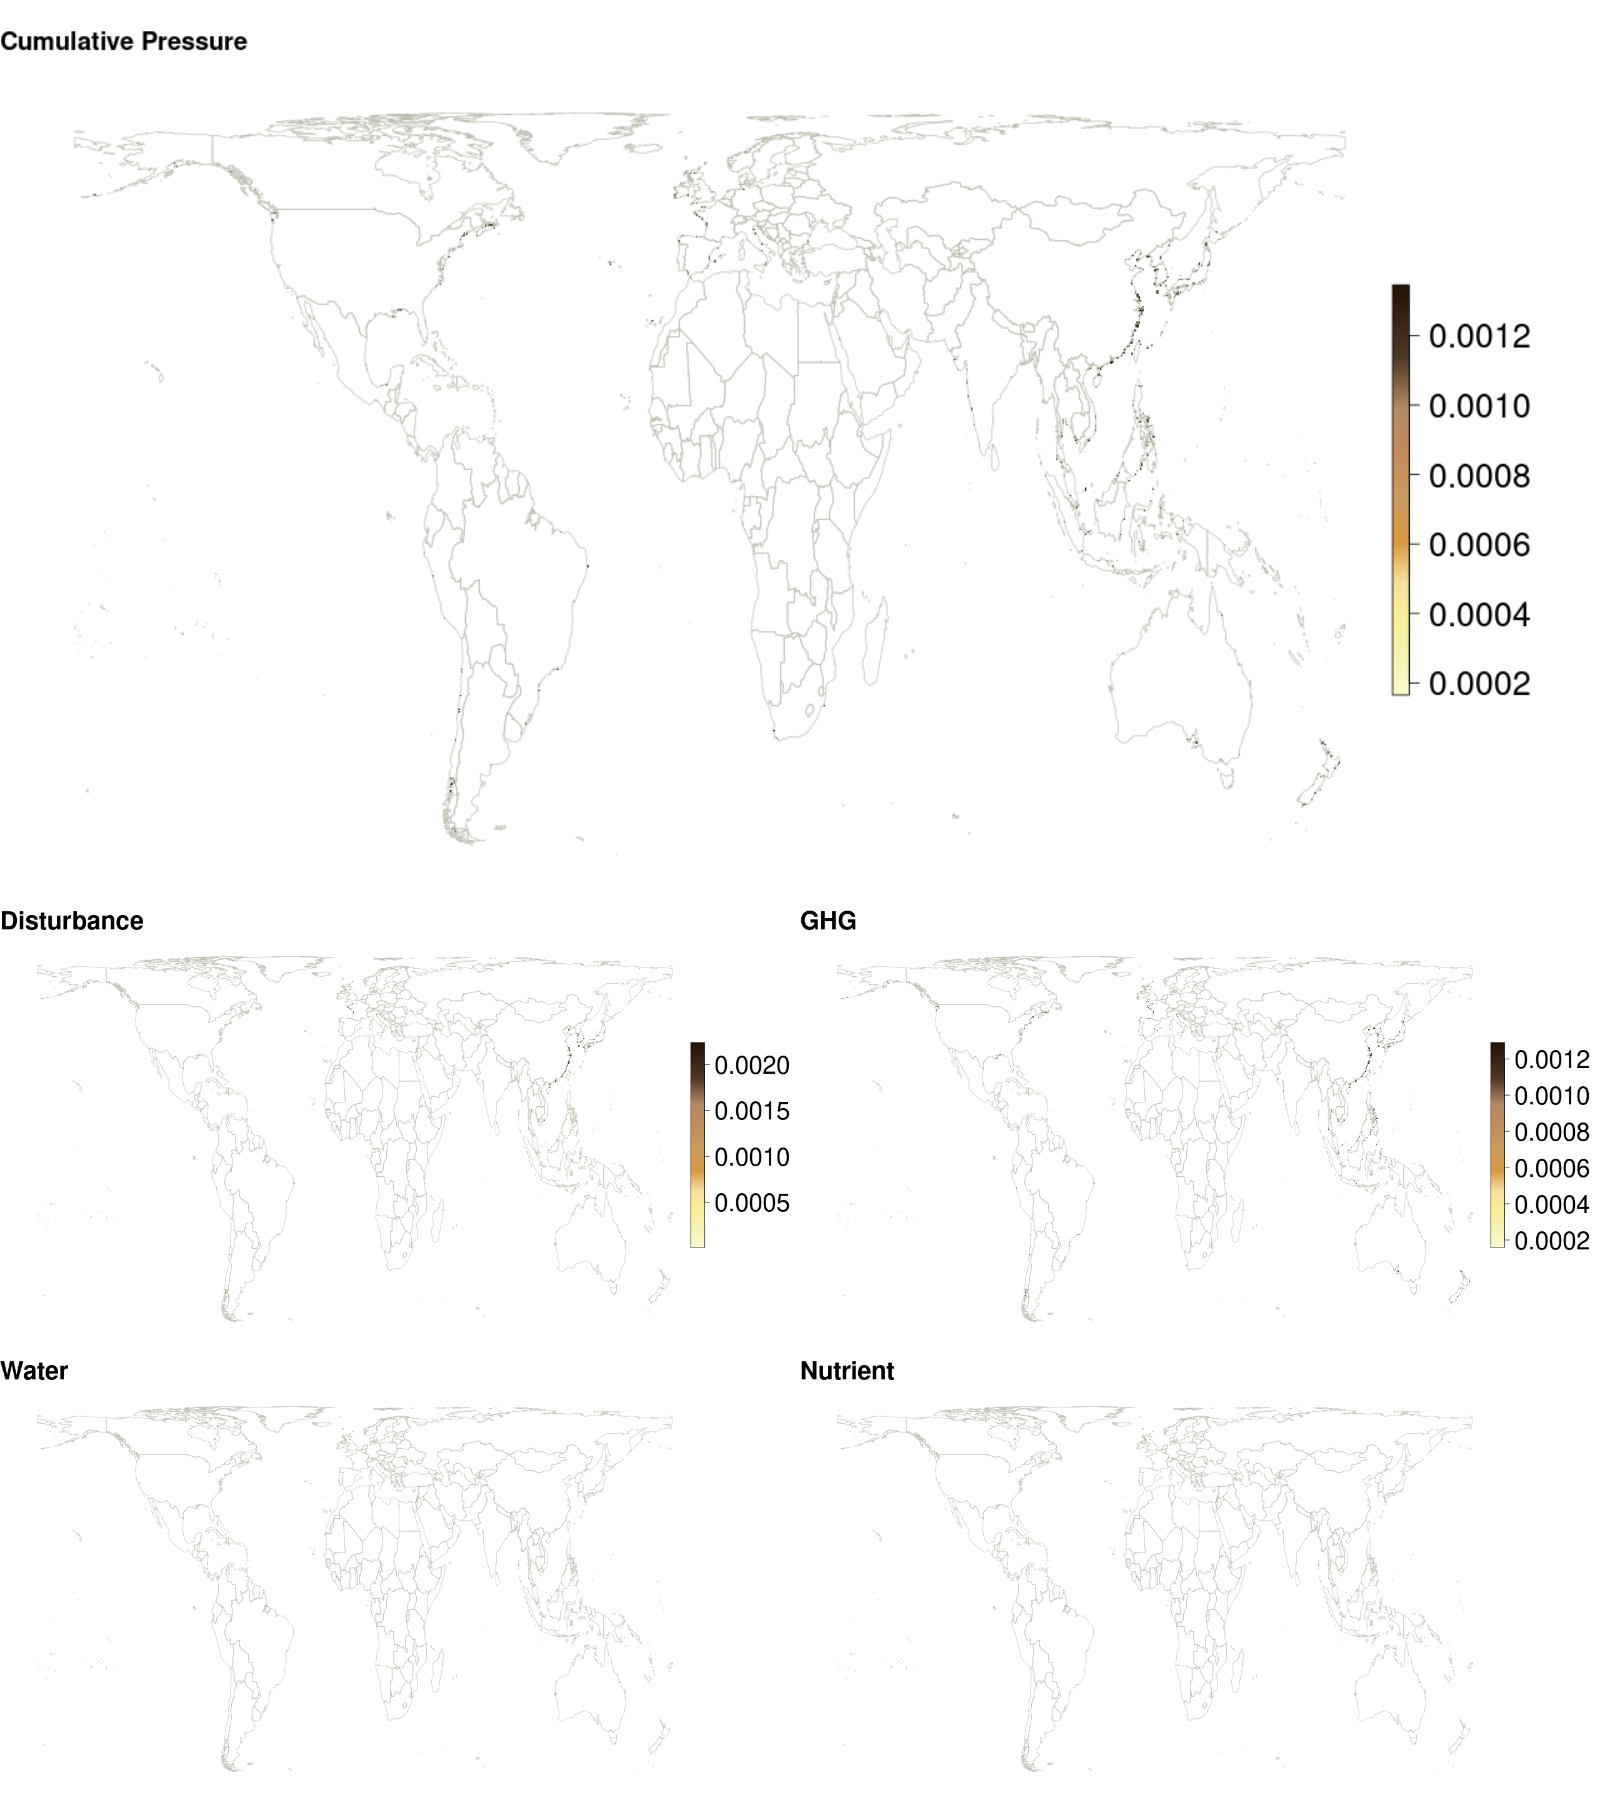
\includegraphics{/home/rayner/food-systems/_analysis/figures/extended_data/output/ed_fig_1_png/bivalve_aquaculture_final.png}

\begin{center}\rule{0.5\linewidth}{0.5pt}\end{center}

\hypertarget{crustaceans-aquaculture}{%
\subparagraph{2) Crustaceans
aquaculture}\label{crustaceans-aquaculture}}

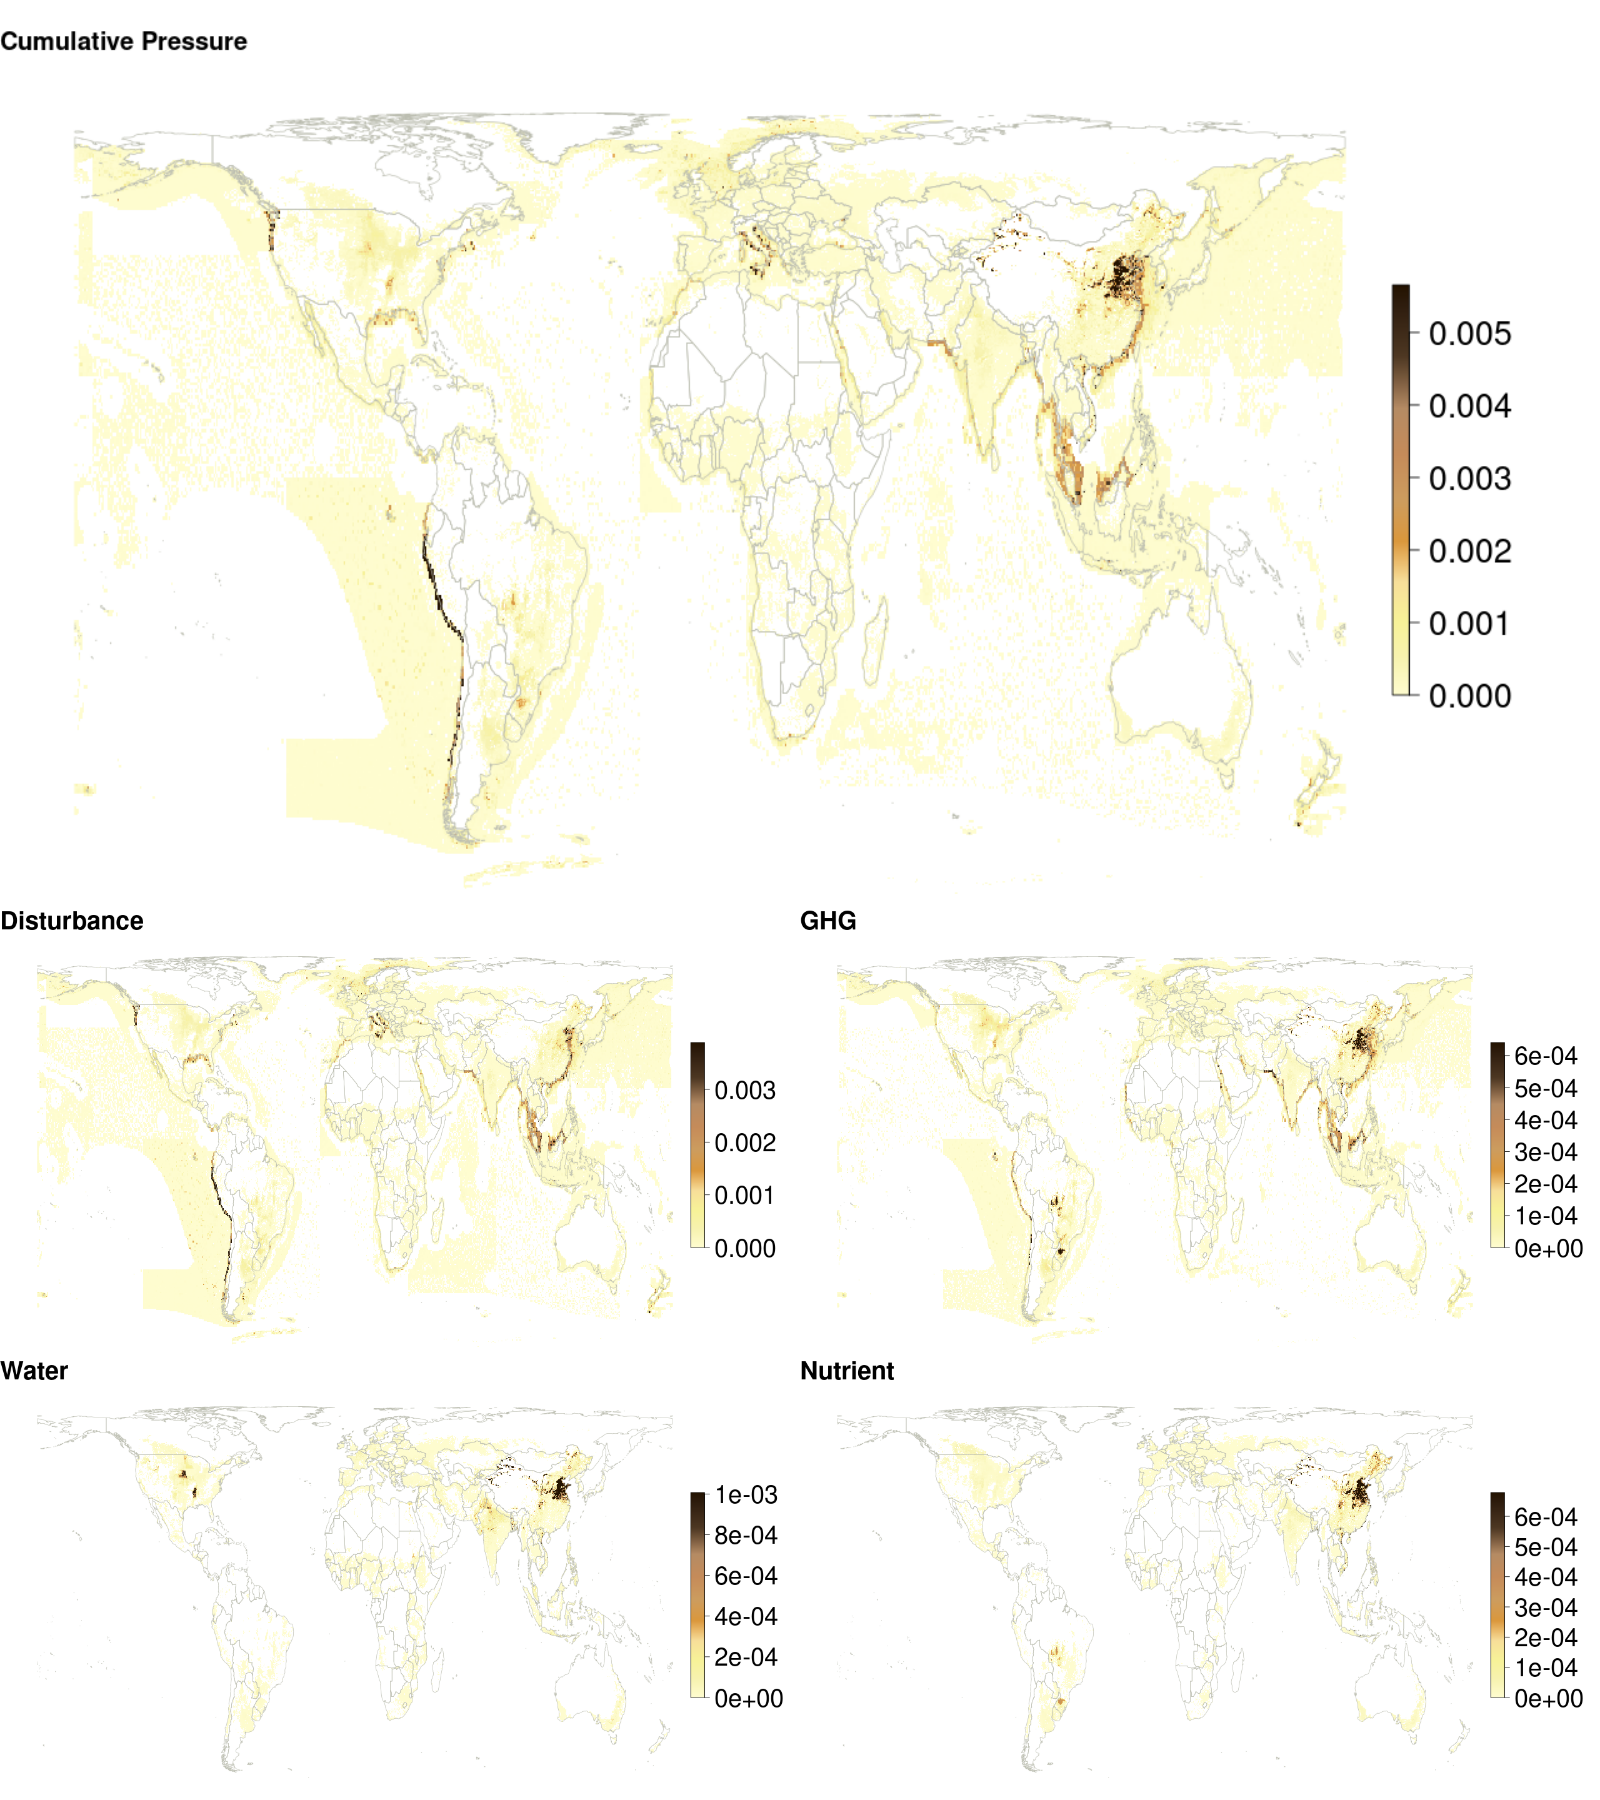
\includegraphics{/home/rayner/food-systems/_analysis/figures/extended_data/output/ed_fig_1_png/crustaceans_aquaculture_final.png}

\begin{center}\rule{0.5\linewidth}{0.5pt}\end{center}

\hypertarget{marine-fish-general-aquaculture}{%
\subparagraph{3) Marine fish general
aquaculture}\label{marine-fish-general-aquaculture}}

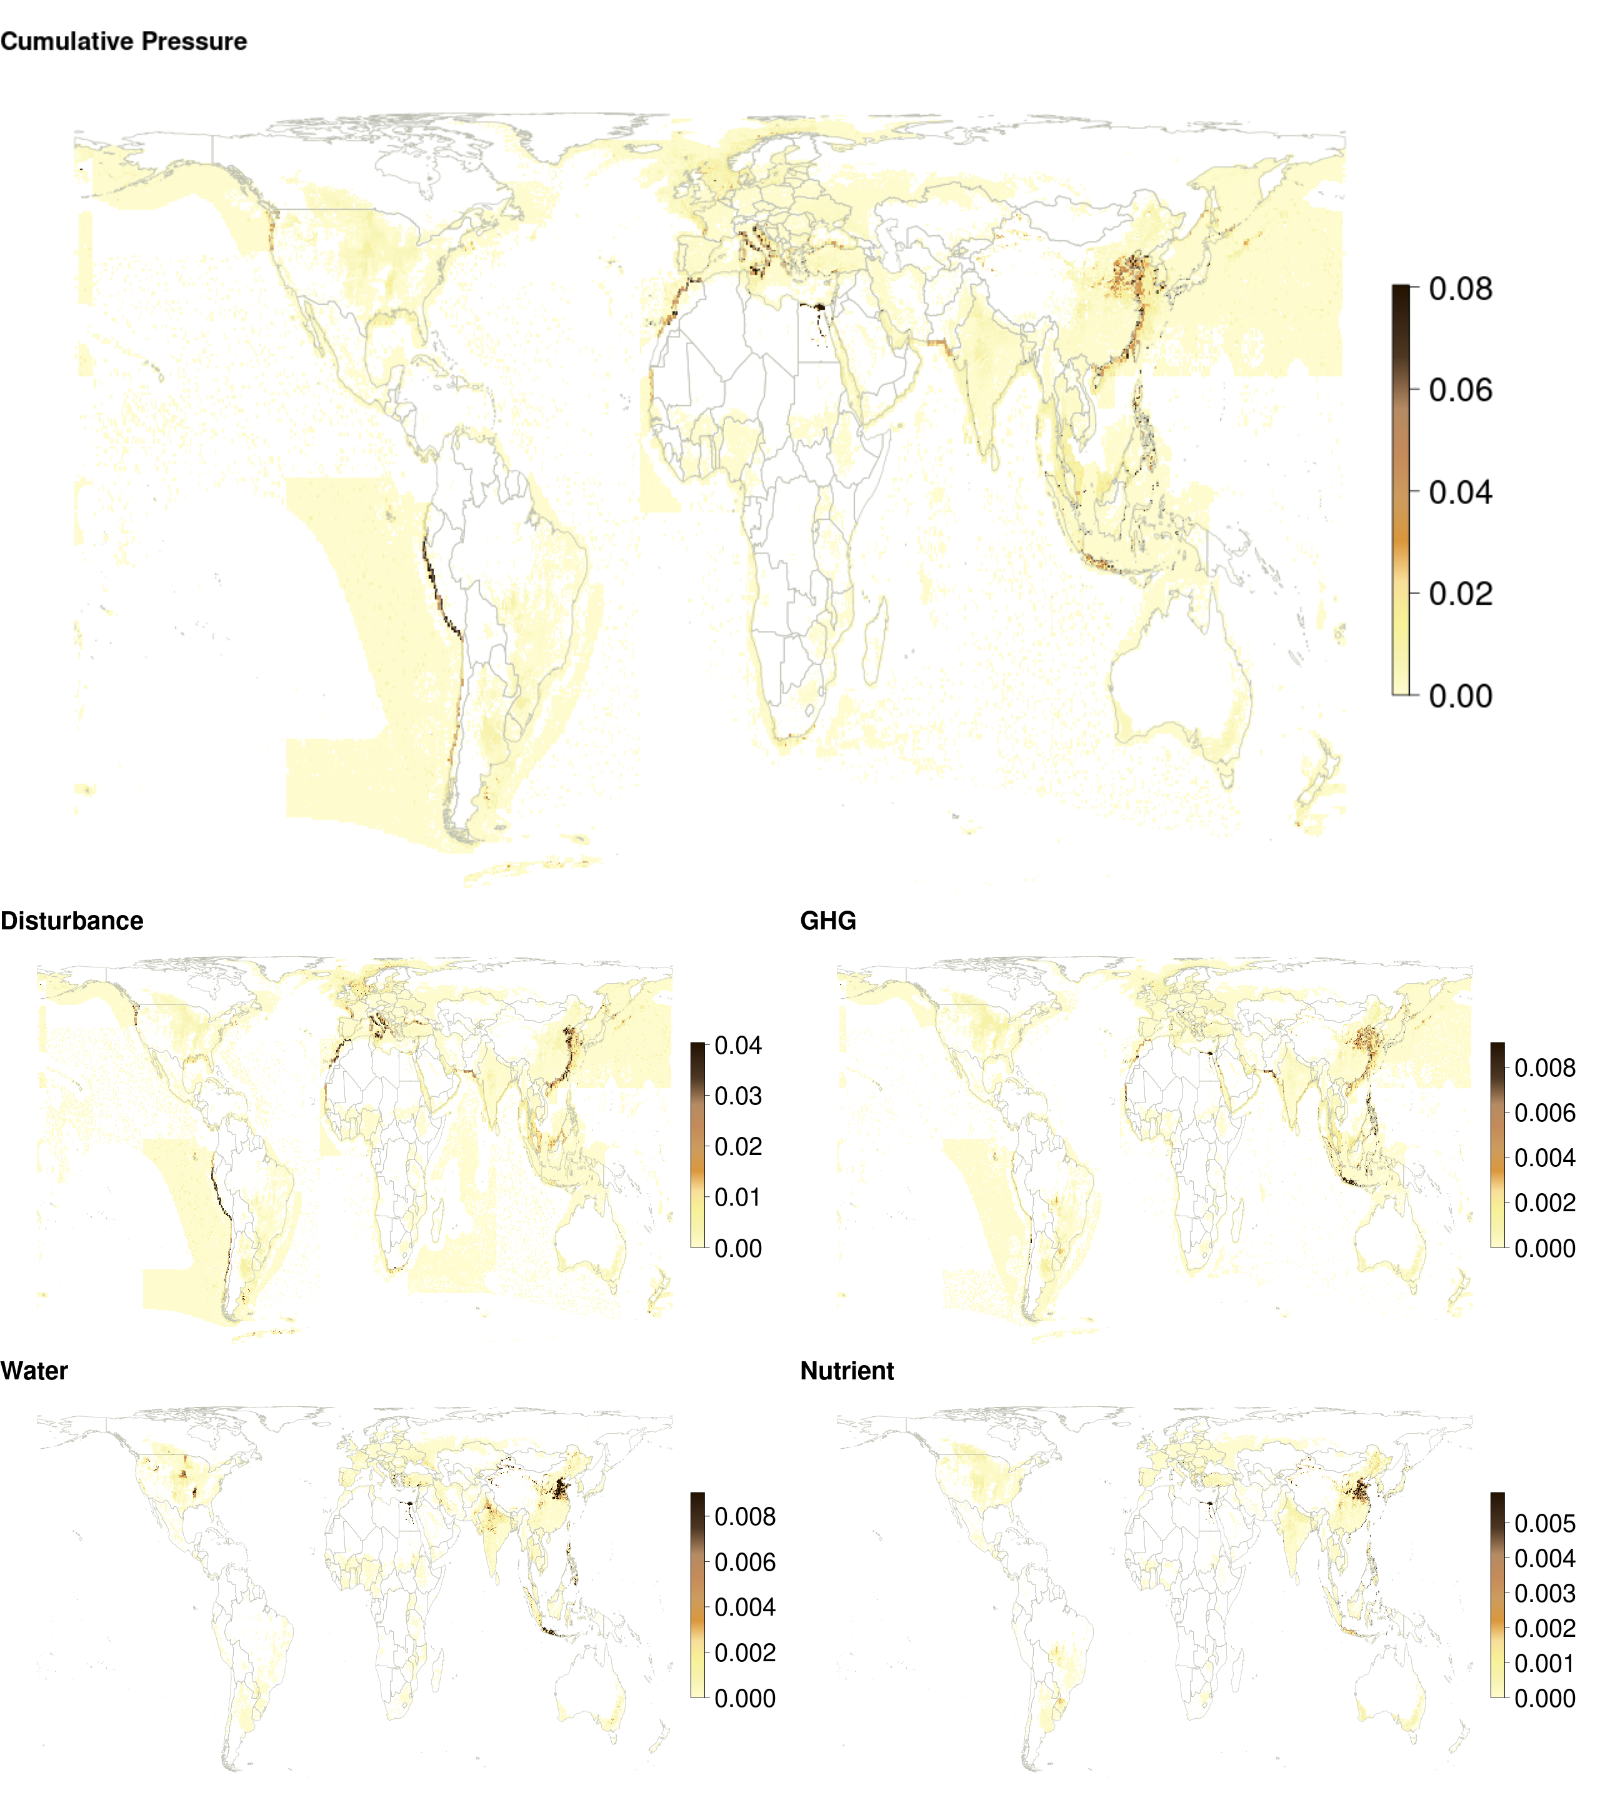
\includegraphics{/home/rayner/food-systems/_analysis/figures/extended_data/output/ed_fig_1_png/marine-fish-general_aquaculture_final.png}

\begin{center}\rule{0.5\linewidth}{0.5pt}\end{center}

\hypertarget{salmon-aquaculture}{%
\subparagraph{4) Salmon aquaculture}\label{salmon-aquaculture}}

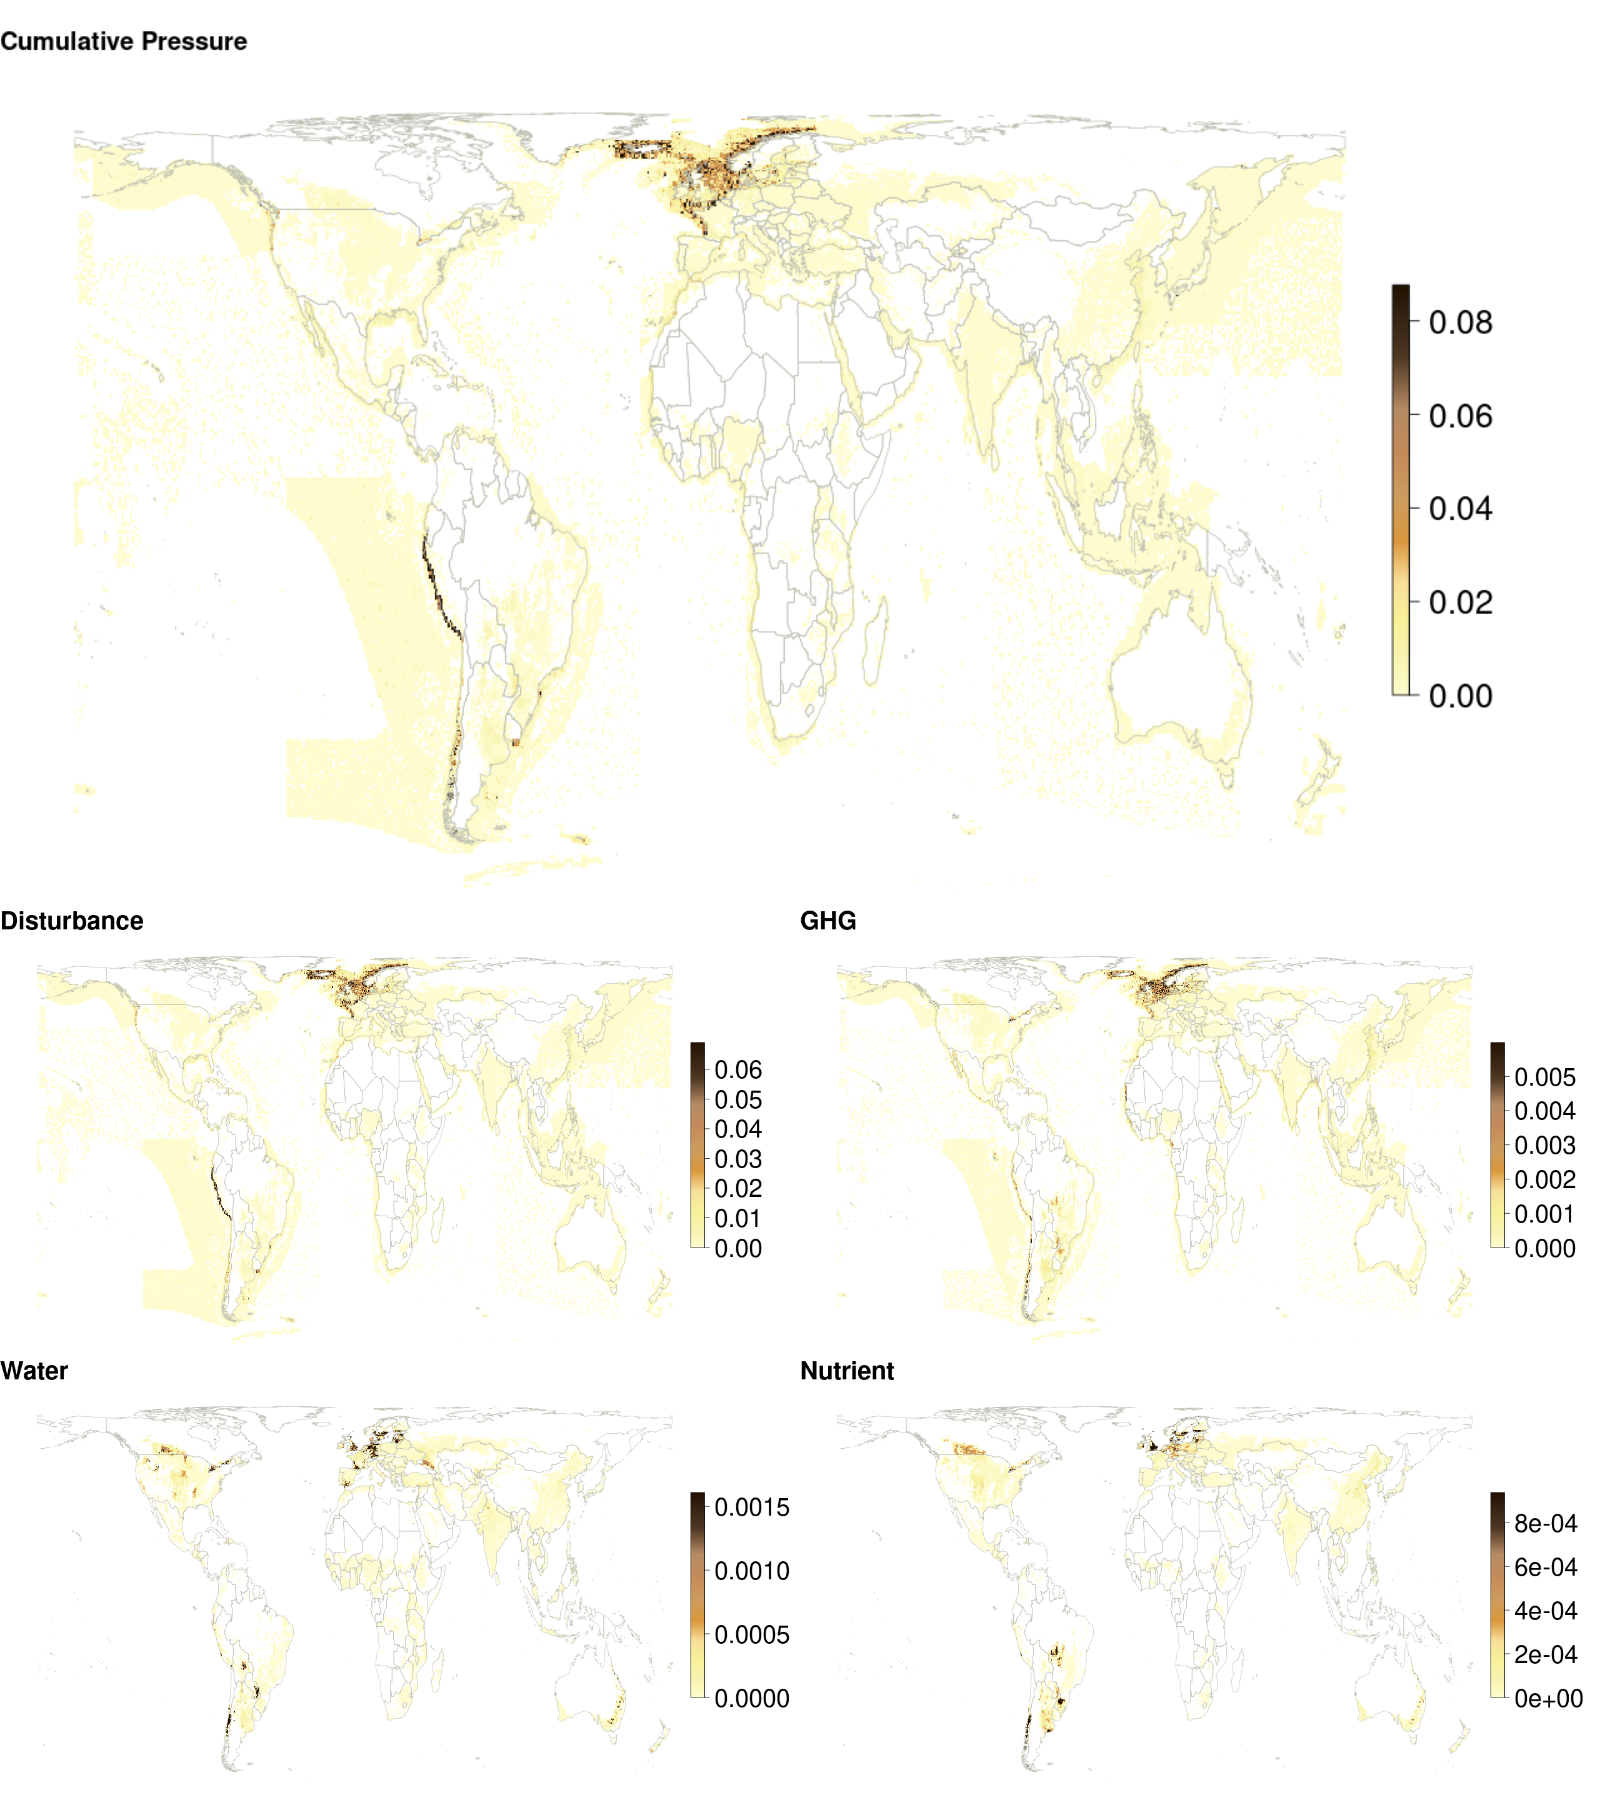
\includegraphics{/home/rayner/food-systems/_analysis/figures/extended_data/output/ed_fig_1_png/salmon_aquaculture_final.png}

\begin{center}\rule{0.5\linewidth}{0.5pt}\end{center}

\hypertarget{shrimp-aquaculture}{%
\subparagraph{5) Shrimp aquaculture}\label{shrimp-aquaculture}}

\includegraphics{/home/rayner/food-systems/_analysis/figures/extended_data/output/ed_fig_1_png/shrimp_aquaculture_final.png}

\begin{center}\rule{0.5\linewidth}{0.5pt}\end{center}

\hypertarget{tuna-aquaculture}{%
\subparagraph{6) Tuna aquaculture}\label{tuna-aquaculture}}

\includegraphics{/home/rayner/food-systems/_analysis/figures/extended_data/output/ed_fig_1_png/tuna_aquaculture_final.png}

\begin{center}\rule{0.5\linewidth}{0.5pt}\end{center}

\end{document}
